%Este trabalho está licenciado sob a Licença Creative Commons Atribuição-CompartilhaIgual 3.0 Não Adaptada. Para ver uma cópia desta licença, visite https://creativecommons.org/licenses/by-sa/3.0/ ou envie uma carta para Creative Commons, PO Box 1866, Mountain View, CA 94042, USA.

%%%%%%%%%%%%%%%%%%%%%%%%%%%%%%%%%%%%%%%%%%
% ATENÇÃO
%
% POR SEGURANÇA, NÃO EDITE ESTE ARQUIVO
%
%%%%%%%%%%%%%%%%%%%%%%%%%%%%%%%%%%%%%%%%%

\documentclass[12pt]{book}

\input preambulo.tex

\makeindex

\begin{document}

\frontmatter

\title{Álgebra Linear\\\small{Um Livro Colaborativo}}
\author{}
\date{\today}
\ifisbook
\else
\addcontentsline{toc}{chapter}{Capa}
\fi

\maketitle

\include{organizadores}
%Este trabalho está licenciado sob a Licença Creative Commons Atribuição-CompartilhaIgual 3.0 Não Adaptada. Para ver uma cópia desta licença, visite http://creativecommons.org/licenses/by-sa/3.0/ ou envie uma carta para Creative Commons, PO Box 1866, Mountain View, CA 94042, USA.

%%%%%%%%%%%%%%%%%%%%%%%%%%%%%%%%%%%%%%%
%
% ATENÇÃO
%
%POR SEGURANÇA, NÃO EDITE ESTE ARQUIVO
%
%%%%%%%%%%%%%%%%%%%%%%%%%%%%%%%%%%%%%%%

\chapter*{Colaboradores}
\addcontentsline{toc}{chapter}{Colaboradores}

Este material é fruto da escrita colaborativa. Veja a lista de colaboradores em:
\begin{center}
  \url{https://github.com/reamat/AlgebraLinear/graphs/contributors}
\end{center}

Para saber mais como participar, visite o site oficial do projeto:
\begin{center}
  \url{https://www.ufrgs.br/reamat/AlgebraLinear}
\end{center}
ou comece agora mesmo visitando nosso repositório GitHub:
\begin{center}
  \url{https://github.com/reamat/AlgebraLinear}
\end{center}

\include{licenca}
%Este trabalho est� licenciado sob a Licen�a Creative Commons Atribui��o-CompartilhaIgual 3.0 N�o Adaptada. Para ver uma c�pia desta licen�a, visite http://creativecommons.org/licenses/by-sa/3.0/ ou envie uma carta para Creative Commons, PO Box 1866, Mountain View, CA 94042, USA.

\chapter*{Nota dos organizadores}
\addcontentsline{toc}{chapter}{Nota dos organizadores}

Este livro � parte de nosso projeto de escrita colaborativa de recursos educacionais abertos. Nosso objetivo � produzir um material did�tico no n�vel de gradua��o de excelente qualidade e de acesso livre pela colabora��o entre professores e alunos de universidades, institutos de educa��o e demais interessados em t�picos de �lgebra linear.

O sucesso deste projeto depende da colabora��o! Edite voc� mesmo o livro, d� sugest�es ou nos avise de erros e imprecis�es. Toda a colabora��o � bem vinda. Saiba mais visitando o reposit�rio oficial do livro:
\begin{center}
  \url{https://fithub.com/livroscolaborativos/AlgebraLinear}
\end{center}

Desejamos-lhe �timas colabora��es!

\include{prefacio}

\ifisbook
\tableofcontents
\addcontentsline{toc}{chapter}{Sumário}
\fi

\mainmatter

%Este trabalho está licenciado sob a Licença Creative Commons Atribuição-CompartilhaIgual 3.0 Não Adaptada. Para ver uma cópia desta licença, visite https://creativecommons.org/licenses/by-sa/3.0/ ou envie uma carta para Creative Commons, PO Box 1866, Mountain View, CA 94042, USA.

%\documentclass[../livro.tex]{subfiles} %%DM%%Escolher document class and options article, etc

%define o diretório principal
\providecommand{\dir}{..}

%%%%%%%%%%%%%%%%%%%%%%%%%%%%%%%%%%%%%%%%%%%%%
%%%%%%%%%%%%INICIO DO DOCUMENTO%%%%%%%%%%%%%%
%%%%%%%%%%%%%%%%%%%%%%%%%%%%%%%%%%%%%%%%%%%%%

%\begin{document}

%\maketitle
%\tableofcontents

% \section{Estrutura do Curso}

% Ver plano de ensino e/ou plataforma Moodle.

\chapter{Semana 1}

\section{Sistemas Lineares}

{\bf Definições Básicas}

\bigskip

\begin{defn} Uma equação é dita {\bf linear } se for do tipo
\[
a_1 x_1 + a_2 x_2 + \hdots + a_n x_n = b
\]
onde $a_1, a_2 , \hdots, \ a_n$ são constantes chamadas coeficientes, $b$ é uma constante chamada termo independente e $x_1, x_2 , \hdots \ x_n$ são as variáveis ou incógnitas. Aqui $n$ é o  número de variáveis e pode ser qualquer número natural.
\end{defn}

\bigskip

\begin{ex}
A equação abaixo
\[
3 x_1 + 5 x_2 - x_3 = 7
\] é uma equação linear nas variáveis $x_1, x_2$ e $x_3$ com coeficientes 3,5, e -1 e termo independente 7.
\end{ex}


\begin{ex}
A equação abaixo também é linear
\[
2x+3y-5z+2w=11
\]
com coeficientes 2,3,-5,2, termo independente 11 e variáveis x, y, z e w.
\end{ex}

\begin{ex}
A seguir temos um exemplo diferente,
\[
5x+3z+14=y+3x-11
\] que é uma equação linear mas não está escrita na forma usual. Note que ela pode ser reescrita como
\[
2x-y+3z=-25
\]
e dessa maneira vemos que ela tem coeficientes 2,-1, e 3,  termo independente 25 e envolve as variáveis x, y, z.
\end{ex}

\begin{ex} As equações abaixo {\bf não} são lineares:

\[x+3y-z^2=5,\]
\[xy = 1,\]
\[sen(x)=\frac{1}{3}, \]
\[(1.02)^x=2.\]
\end{ex}

\begin{defn} Um sistema de equações lineares (ou sistema linear - SL) é uma coleção finita de equações lineares envolvendo um certo conjunto finito de  variáveis.
\end{defn}

\begin{ex}
O sistema linear
\begin{equation*}
\left\{
\begin{array}{ccccccc}
2x&+&3y&-&z&=&7 \\
x&+&8y& & &=&0
\end{array}
\right.
\end{equation*}
é um exemplo de SL de ordem $2 \times 3$, ou seja tem 2 equações e 3 variáveis. Note que a variável z tem coeficiente zero na segunda equação.
\end{ex}


\begin{ex}
O sistema linear
\begin{equation*}
\left\{
\begin{array}{ccccccccc}
x&+&2y&-&3z& & &=&22 \\
x& &  &+&z & & &=&17 \\
&-&y & &  &+&2w&=&6 \\
\end{array}
\right.
\end{equation*}
é um exemplo de SL de ordem $3 \times 4$, ou seja três equações nas variáveis x, y, z, w.
\end{ex}


\begin{ex}
Aqui vale também a observação de que um SL pode aparecer de forma "desorganizada", ou seja, a ordem em que as variáveis aparecem nas equações pode ser diferente de uma equação para outra e as variáveis podem aparecer mais de uma vez. O termo independente também pode aparecer do lado esquerdo da igualdade, ou estar parte a esquerda e parte a direita.
Por exemplo,

\begin{equation*}
\left\{
\begin{array}{ccc}
2z-3x+1 & = &y \\
x+4z+3& = & 3x+2z+2y-7.
\end{array}
\right.
\end{equation*}

Veremos que para resolvermos um sistema linear será fundamental reescrevê-lo na forma usual. O sistema dado acima poderia ser reescrito como:

\begin{equation*}
\left\{
\begin{array}{ccc}
-3x-y+2z & = & -1 \\
-2x-2y-2z & = & -10,
\end{array}
\right.
\end{equation*}
ou ainda na forma
\begin{equation*}
\left\{
\begin{array}{ccc}
3x+y-2z & = & 1 \\
x+y-z & = & 5.
\end{array}
\right.
\end{equation*}
\end{ex}

Note que se qualquer equação do sistema for não-linear, então o sistema não pode ser considerado um SL.
Neste texto iremos analisar técnicas de resolução de sistemas lineares apenas. Sistemas não-lineares têm tratamento matemático muito mais difícil e fogem do escopo deste texto.


\bigskip

\begin{defn}  Uma solução de um sistema linear nas variáveis $x_1, x_2 , \hdots \ x_n$
é uma %lista  de valores numéricos que fazem com que todas as equações do SL sejam verificadas quando as variáeis s
atribuição de valores
às variáveis que verificam (ou satisfazem) todas as equações do sistema.
\end{defn}

\begin{ex}
O sistema linear
\begin{equation*}
\left\{
\begin{array}{ccccc}
x&+&y&=&5 \\
3x&-&y&=&-1
\end{array}
\right.
\end{equation*}
tem $x=1$ e $y=4$ como solução.

\end{ex}

\bigskip

\begin{defn}  O conjunto solução de um SL (ou a solução de um SL) é o conjunto formado por todas as soluções individuais (no sentido da definição anterior) deste SL.
\end{defn}

\begin{ex} Vamos estudar sistemas lineares $2 \times 2$ fazendo uso de uma interessante interpretação geométrica.
O conjunto solução de um sistema linear
\begin{equation*}
\left\{
\begin{array}{ccccc}
a_1 x&+&b_1 y&=&c_1 \\
a_2 x&+&b_2 y&=&c_2 \\
\end{array}
\right.
\end{equation*}
é dado, geometricamente, pela intersecção das retas representativas das duas equações acima.

Assim sendo, temos três possibilidades

{\bf Sistemas Lineares compatíveis e Determinados}, aqueles que apresentam uma única solução: no caso $2 \times 2$ ocorre quando as duas retas tem inclinações distintas, não sendo portanto paralelas, e interseccionando-se em um único ponto. Por exemplo
\begin{equation*}
\left\{
\begin{array}{ccccc}
x&+& y&=&1 \\
2 x&+& y&=&8. \\
\end{array}
\right.
\end{equation*}

{\bf Sistemas Lineares compatíveis e Indeterminados}, aqueles que apresentam infinitas soluções: no caso $2 \times 2$ ocorre quando as duas retas são idênticas, e a intersecção de ambas é a própria reta.
Por exemplo
\begin{equation*}
\left\{
\begin{array}{ccccc}
2 x&+& y&=&1 \\
4 x&+& 2 y&=& 2. \\
\end{array}
\right.
\end{equation*}

{\bf Sistemas incompatíveis}, aqueles que não tem solução: no caso $2 \times 2$ ocorre quando as duas retas são paralelas, mas distintas, e a intersecção entre elas é o conjunto vazio.
Por exemplo
\begin{equation*}
\left\{
\begin{array}{ccccc}
x&+& y&=&1 \\
x&+& y&=&3. \\
\end{array}
\right.
\end{equation*}

Os sistemas incompatíveis também são chamados de sistemas impossíveis.

\end{ex}

Feita esta introdução aos  sistemas lineares, surge a pergunta natural: como obter a solução de tais sistemas?
Começamos com um exemplo:


\begin{ex}
Considere o sistema linear que consiste de duas equações e duas variáveis
\begin{equation}\label{exp1}
  \left\{
    \begin{array}{rcl}
      x+3y&=&1 \\
      2x-y&=&-2.
    \end{array}
  \right.
  \end{equation} %Nosso objetivo é descobrir o valor (ou todos os valores) das variáveis $x$ e $y$ que satisfazem a ambas equações.

\vspace{0.2cm}

\noindent\textit{Solução 1.} Ao multiplicar toda a primeira equação por $-2$, não alteramos a solução do sistema, pois, caso quiséssemos voltar ao sistema original, bastaria dividir a primeira equação do sistema abaixo por $-2$. Ficamos assim com o sistema
\begin{equation}
  \left\{
    \begin{array}{rcl}
      -2x-6y&=&-2 \\
      2x-y&=&-2.
    \end{array}
  \right.
\end{equation} Em seguida, somamos as duas equações e mantemos uma delas.
\begin{equation}
  \left\{
    \begin{array}{rcl}
      -2x-6y&=& -2 \\
      -7y & =& -4.
    \end{array}
  \right.
\end{equation} Este sistema também tem as mesmas soluções do anterior, pois podemos a qualquer hora retornar ao sistema original fazendo $($linha 2$)-($linha 1$)$.

Em verdade, manter a equação da primeira linha multiplicada por $-2$ não ajuda em nada na resolução do sistema e voltaremos à equação original. Além disso, na linha dois já podemos isolar a variável $y$ e descobrir o seu valor. Ficamos então com o sistema:
\begin{equation}\label{exp1-2}
  \left\{
    \begin{array}{rcl}
      x+3y&=& 1 \\
      -7y & =& -4.
    \end{array}
  \right.
\end{equation}

Observamos, finalmente, que a solução do último sistema (que é a mesma do sistema original) já está muito fácil de ser obtida. Sabemos o valor de $y$ pela segunda equação e, para descobrir o valor de $x$, basta usar a primeira equação:
\begin{equation}
y = \frac{4}{7} \implies x + 3\cdot \frac{4}{7} = 1 \implies x = 1 - \frac{12}{7} = - \frac{5}{7}.
\end{equation} Podemos escrever a solução do sistema como
\begin{equation}
  \left\{
    \begin{array}{rcl}
      x&=&-5/7 \\
      y&=& \ \ 4/7
    \end{array}
  \right. \lhd
\end{equation}
\end{ex}

O símbolo $\lhd$ acima nas nossas notas indica o fim de uma solução, exemplo ou observação.

Em seguida, fazemos algumas observações.

\begin{obs}
O sistema linear como o acima possui duas equações e duas variáveis e por isto é conhecido como um sistema linear $2\times 2$ (lê-se dois por dois). Mais geralmente, um sistema linear com $m$ equações e $n$ variáveis é conhecido como um sistema linear $m \times n$ (lê-se $m$ por $n$).
\end{obs}

\begin{obs}
Sistemas $2\times 2$ são dos mais simples de resolver e por isso o método acima pode parecer desnecessariamente complicado. Mas, como veremos, este método pode ser aplicado para qualquer sistema. Logo, é essencial que se entenda completamente todos os seus passos para um bom acompanhamento do que está por vir.
\end{obs}

Vamos analisar a solução apresentada acima mais de perto. Para irmos do sistema linear em \eqref{exp1} para o sistema em \eqref{exp1-2}, fizemos uma sequência de operações que:
\begin{itemize}
  \item \emph{não alteram a solução do sistema linear original ;}
  \item resumidamente, podem ser descritas como \emph{adicionar um múltiplo da linha um na linha dois.}
\end{itemize} Que a solução permanece a mesma pode ser justificado tal qual está na ``Solução 1'' acima.

\vspace{0.2cm}

Operações nas linhas de um sistema que não alteram o conjunto de soluções são chamadas de \textbf{operações elementares}. São as seguintes:
\begin{enumerate}
  \item Multiplicar uma linha por uma constante não nula;
  \item Trocar duas linhas de lugar;
  \item Substituir uma linha por esta mesma linha somada com um múltiplo de outra linha.
  %Somar um múltiplo de uma linha a outra linha.
\end{enumerate}

\vspace{0.2cm}

Um artifício que torna todo o processo mais ``automático'' é o de formar uma tabela de números com os coeficientes do sistema:
\begin{equation}
  \left\{
    \begin{array}{rcl}
      x+3y&=&1 \\
      2x-y&=&-2
    \end{array}
  \right. \qquad \rightsquigarrow \qquad  \left[
                             \begin{array}{cc|c}
                               1 & 3 & 1 \\
                               2 & -1 & -2.
                             \end{array}
                           \right]
\end{equation} A tabela de números da direita é conhecida como a \textbf{matriz aumentada associada ao sistema linear}. Vamos nos referir às linhas da matriz associada como $\ell_1$ e $\ell_2$. Deste modo, ``adicionar um múltiplo da linha 1 na linha dois'' corresponde a fazer:
\begin{equation}
\left[
                             \begin{array}{cc|c}
                               1 & 3 & 1 \\
                               2 & -1 & -2
                             \end{array}
                           \right] \quad \xrightarrow{-2\ell_1 + \ell_2 \text{ em } \ell_2} \quad
\left[
                             \begin{array}{cc|c}
                               1 & 3 & 1 \\
                               0 & -7 & -4.
                             \end{array}
                           \right]
\end{equation} Para este tipo de operação, olhamos para as colunas da matriz associada, fizemos mentalmente (ou em uma folha de rascunho) os cálculos envolvidos e preenchemos os valores na respectiva linha da nova matriz que está à direita:
\begin{equation}
(-2)\cdot 1 + 2 = 0, \qquad (-2)\cdot 3 + (-1) = -7, \qquad (-2) \cdot 1 + (-2) = -4.
\end{equation}



\begin{ex}\label{exemplo3por3}
Consideramos agora um sistema com três equações e três variáveis;
\begin{equation}
\left\{
  \begin{array}{ll}
    x + 2y + z = 12 \\
    x -3y + 5z = 1 \\
    2x - y + 3z = 10.
  \end{array}
\right.
\end{equation} Vamos diretamente escrever a matriz aumentada associada ao sistema, que é a matriz com os coeficientes da variável $x$ na primeira coluna, os coeficientes da variável $y$ na segunda coluna, os coeficientes de $z$ na terceira coluna e os coeficientes independentes na última coluna:
\begin{equation}
\left[
  \begin{array}{ccc|c}
    1 &  2 & 1 & 12 \\
    1 & -3 & 5 & 1 \\
    2 & -1 & 3 & 10.
  \end{array}
\right]
\end{equation} Em seguida, utilizamos operações elementares nas linhas como no exemplo anterior. Ao substituir $-\ell_1 + \ell_2$ em $\ell_2$, obtemos
\begin{equation}
\left[
  \begin{array}{ccc|c}
    1 &  2 & 1 & 12 \\
    0 & -5 & 4 & -11 \\
    2 & -1 & 3 & 10 .
  \end{array}
\right]
\end{equation} Ou seja, eliminamos o valor $1$ da primeira posição da segunda linha (em outras palavras, eliminamos a variável $x$ da segunda equação). Prosseguindo com a eliminação dos valores abaixo da diagonal principal da matriz, obtemos:
\begin{equation}
\left[
  \begin{array}{ccc|c}
    1 &  2 & 1 & 12 \\
    0 & -5 & 4 & -11 \\
    2 & -1 & 3 & 10
  \end{array}
\right]
\quad \xrightarrow{-2\ell_1 + \ell_3 \text{ em } \ell_3} \quad
\left[
  \begin{array}{ccc|c}
    1 &  2 & 1 &  12 \\
    0 & -5 & 4 & -11 \\
    0 & -5 & 1 & -14
  \end{array}
\right]
\quad \xrightarrow{-\ell_2 + \ell_3 \text{ em } \ell_3} \quad
\left[
  \begin{array}{ccc|c}
    1 &  2 &  1 &  12 \\
    0 & -5 &  4 & -11 \\
    0 &  0 & -3 & -3.
  \end{array}
\right]
\end{equation} Voltando à notação original do sistema, obtemos
\begin{equation}
\left\{
  \begin{array}{llll}
    x &+ 2y &+ z &= 12 \\
      &- 5y &+ 4z &= -11 \\
      &    &- 3z& = -3
  \end{array}
\right.
\end{equation} Por causa do seu formato, este sistema é dito estar em \textbf{forma triangular} ou ainda que o sistema é \textbf{triangular}.

Como já tínhamos percebido no nosso primeiro exemplo, sistemas triangulares são fáceis de resolver. Pela última equação concluímos que $z=1$. Substituindo este valor na segunda equação, obtemos:
\begin{equation}
- 5y + 4 = -11 \implies y = 3.
\end{equation}
Finalmente, substituindo estes dois valores na primeira equação, obtemos:
\begin{equation}
x + 2\cdot 3 + 1 = 12 \implies x=5.
\end{equation}
Portanto, a solução para o sistema é $(x,y,z) = (5,3,1). \lhd$
\end{ex}


Esta técnica de resolver sistemas lineares é importante por ser aplicável a sistemas de qualquer ordem e é conhecida como \textbf{escalonamento} ou \textbf{eliminação Gaussiana}.

\subsection*{Exercícios resolvidos}

\construirExeresol

\begin{exeresol}
Resolva o sistema linear abaixo usando sua matriz aumentada associada.
\begin{equation}
  \left\{
    \begin{array}{rcl}
      -5x+2y&=&3 \\
      9x+y&=&2
    \end{array}
  \right..
\end{equation}
\end{exeresol}
\begin{resol}
Para resolver esse problema, basta fazermos como antes, escrevemos os coeficientes de cada variável na matriz:
\begin{equation}
 \left[
  \begin{array}{cc|c}
    -5 &  2 & 3 \\
    9 & 1 & 2
  \end{array}
\right]
\end{equation}
Feito isso, basta fazer as operações elementares:
\begin{equation}
 \left[
  \begin{array}{cc|c}
    -5 &  2 & 3 \\
    9 & 1 & 2
  \end{array}
\right]
\quad \xrightarrow{9\ell_1 + 5\ell_2 \text{ em } \ell_2} \quad
 \left[
  \begin{array}{cc|c}
    -5 &  2 & 3 \\
    0 & 23 & 37
  \end{array}
\right]
\end{equation}
Obtemos então:
\begin{equation}
23y = 37 \implies y = \frac{37}{23}
\end{equation}
Por fim, substituímos o valor encontrado de $y$ na primeira equação:
\begin{equation}
 -5x + 2\cdot \frac{37}{23} = 3 \implies x = \frac{1}{23}
\end{equation}
Feito isso, temos que a solução do problema é $(x,y) = (\frac{1}{23}, \frac{37}{23}) \lhd$.
\end{resol}
\begin{exeresol}
        Demonstre que é ou não é linear:
        \justify
            \begin{enumerate}
                \item $x^{2}$
                \item $a*x + b = 0$
                \item $(x + k)^{2}$
                \item $e^{x}$
            \end{enumerate}
\end{exeresol}
\begin{resol}
        \begin{flushleft}
        Para resolvermos a questão nos remetemos a definição de linearidade e as proriedade das funções lineares,
        que seria a aditividade() e : $f(x) + f(x^{'}) = f(x + x^{'})$
        e homogeniedade : $a*f(x) = f(a*x)$.
        \end{flushleft}
        \begin{flushleft}
            \begin{enumerate}
                \item Seja $x^{2}$, não é linear pois $f(x^{2}) + f(x^{2}) \neq f(x + x^{'})^2$ e $a*f(x^{2}) \neq f(a*x)^{2}$.
                \item Seja $a*x + b = 0$, é linear, pois, $f(a*x + b) + f(a*x + b^{'}) = f(a*x + b + (a*x + b)^{'})$ e  $a*f(c*x + b) = f(a*c*x + a*b)$.
                \item Seja $(x + k)^{2}$, não é liner, pois, $f(x + k)^{2} + f(x + k)^{2}) \neq f((x + k) + (x + k)^{'})^2$
            e $a*f(x + k)^{2} \neq f((a*x + a*k)^{2})$.
                \item Seja $e^{x}$, não é linear, pois, $f(e^{x}) + f(e^{x'}) \neq f(e + e)^{x'}$.
            \end{enumerate}
        \end{flushleft}
\end{resol}
\begin{exeresol}
        \begin{flushleft}
        Seja os Sistemas Lineares abaixo, determine se eles são $ \bf { Determinados , Indeterminado}$, ou $\bf{Incompativel}$:
        \end{flushleft}
        \begin{enumerate}
            \item \begin{equation*}
                    \begin{array}{cccccccc}\label{eq:sistema_A}
                        x + y - z = 12 \\
                        3x - 4y + 5z = 40 \\
                        5x - 10y - 3z = 60
                    \end{array}
            \end{equation*}
            \item \begin{equation*}
                    \begin{array}{cccccccc}\label{eq:sistema_B}
                        x + 3y + 5z = 1 \\
                        6x - y + z = 2 \\
                        2x + 3z = 3
                    \end{array}
                \end{equation*}
            \item \begin{equation*}
                \begin{array}{cccccccc}\label{eq:sistema_C}
                    x + 8y = 9  \\
                    64x + 512y = 28
                \end{array}
        \end{equation*}
        \end{enumerate}
\end{exeresol}
\begin{resol}
        \begin{flushleft}
         Para resolver os sistemas lineares foram utilizados a matriz aumentada e a eliminação de Gauss em \ref{eq:sistema_A},
        \ref{eq:sistema_B} e \ref{eq:sistema_C}:
        \end{flushleft}
        \begin{enumerate}
            \item\begin{math}
                    \begin{bmatrix}
                        1 & 1 & 1 & 12 \\
                        3 & -4& 5 & 40 \\
                        5 & 10& -3& 60
                    \end{bmatrix} \\
                        L_{2} \leftarrow L_{2} - 3L_{1}, \\
                        L_{3} \leftarrow L_{3} - 5L_{1} \\
                    \begin{bmatrix}
                        1 & 1 & 1 & 12 \\
                        0 & -7& 2 & 4 \\
                        0 & 5 & -8& 0
                    \end{bmatrix} \\
            \end{math}
             Portanto, o sistema é Indeterminado.
            \item \begin{math}
                    \begin{bmatrix}
                        1 & 3 & 5 & 1 \\
                        6 & 1 & 1 & 2 \\
                        2 & 0 & 3 & 3
                    \end{bmatrix}
                        L_{2} \leftarrow L_{2} - 6L_{1},
                        L_{3} \leftarrow L_{3} - 2L_{1}
                        =
                    \left[\begin{matrix}
                        1 & 3 & 5 & 1 \\
                        0 & -17& -29& -4 \\
                        0 & -6& -7& 1
                    \end{matrix} \right] \\
                        L_{2} \leftarrow -\frac{1}{17}L_{2}
                        =
                    \left[\begin{matrix}
                        1 & 3 & 5 & 1 \\
                        0 & 1 & \frac{29}{17} & \frac{4}{17} \\
                        0 & -6 & -7& 1
                    \end{matrix} \right] \\
                        L_{3} \leftarrow L_{3} - 6L_{2}
                        =
                    \left[\begin{matrix}
                        1 & 1 & 1 & 12 \\
                        0 & 1 & 2 & 4 \\
                        0 & 0 & \frac{55}{17}& \frac{41}{17}
                    \end{matrix} \right] \\
                        L_{3} \leftarrow \frac{17}{55}L_{3}
                        =
                    \left[\begin{matrix}
                        1 & 3 & 5 & 1 \\
                        0 & 1 & \frac{29}{17}& \frac{4}{17} \\
                        0 & 0 & 1 & \frac{41}{55}
                    \end{matrix} \right] \\
                        L_{2} \leftarrow L_{2} -\frac{29}{17}L_{3}
                        =
                    \left[\begin{matrix}
                        1 & 3 & 5 & 1 \\
                        0 & 1 & 0 & \frac{-57}{55} \\
                        0 & 0 & 1 & \frac{41}{55}
                    \end{matrix} \right] \\
                        L_{1} \leftarrow L_{1} - 2L_{2},
                        L_{1} \leftarrow L{1} - 5L_{3}
                        =
                    \begin{bmatrix}
                        1 & 0 & 0 & \frac{21}{55} \\
                        0 & 1 & 0 & \frac{-57}{55} \\
                        0 & 0 & 1 & \frac{41}{55}
                    \end{bmatrix} \\
                \end{math}
        Portanto é um sistema Determinado
            \item\begin{math}
                \begin{bmatrix}
                    1 & 8 & 9 \\
                    64 & 512 & 28
                \end{bmatrix}
                    L_{2} \leftarrow L_{2} - 64L_{1}
                    =
                \begin{bmatrix}
                    1 & 8 & 9 \\
                    0 & 0 & -548
                \end{bmatrix}
                \end{math} \\
        Portanto é um sistema Incompativel.
        \end{enumerate}
 \end{resol}

\subsection*{Exercícios}

\construirExer

\begin{exerc}
        Demostre que se são lineares:
        \begin{itemize}
            \item $x^{100}$
            \item $a*x+c$
            \item $a*x_1 + b_1 +\ldots+ a*x_n + b_n$
            \item $e$
            \item $cos(x)$
        \end{itemize}
\end{exerc}
\begin{exerc}
        Classifique os sistemas abaixo como Determinado, Indeterminado ou Incompativel,
        se Determinado, encontre $x,y,z$:
        \begin{itemize}
            \item \begin{equation}
                        \left\{
                            \begin{array}{rcl}
                                x+y+z&=&10 \\
                                10x+1y+z&=&9 \\
                                x+0y+0z&=&1
                            \end{array}
                        \right..
                   \end{equation}
            \item \begin{equation}
                        \left\{
                        \begin{array}{ccccc|c}
                            3x+2y+1z&=&10 \\
                            6x+8y+2z&=&9 \\
                            1x+\frac{2}{3}y+\frac{1}{3}z&=&1
                        \end{array}
                        \right..
                   \end{equation}
            \item  \begin{equation}
                        \left\{
                            \begin{array}{ccccc|c}
                                1x+2y+1z&=&4 \\
                                2x+8y+2z&=&3 \\
                                8x+2y+8z&=&-18
                            \end{array}
                        \right..
                    \end{equation}
        \end{itemize}
\end{exerc}

\section{Formas escalonadas e formas escalonadas reduzidas}


Vimos dois exemplos de como resolver sistemas lineares por escalonamento. Vamos agora introduzir uma terminologia, esperando tornar o método mais sistemático.

Dizemos que uma matriz está em \textbf{forma escalonada} quando
\begin{enumerate}
  \item As linhas que contém apenas zeros estão abaixo das demais.
  \item O primeiro elemento não nulo de uma linha, conhecido como \textbf{elemento líder}, está em uma coluna à direita do elemento líder da linha acima.
\end{enumerate} Estas duas condições \emph{implicam} que os elementos que estão abaixo de elementos líder são todos iguais a zero.

Por exemplo,
\begin{equation}\label{escalonada1}
\left[
\begin{array}{ccccc}
1 & a_0 & a_1 & a_2 & a_3 \\
0 & 0 & 2 & a_4 & a_5 \\
0 & 0 & 0 & -1 & a_6 \\
0 & 0 & 0 & 0 & 0
\end{array}
\right]
\end{equation} é uma matriz em forma escalonada. Notamos que os coeficientes $a_1, a_2, a_3, a_4, a_5$ e $a_6$ podem ser quaisquer números sem alterar o fato de a matriz estar em forma escalonada.

Outros exemplos, retirados livro do David C. Lay:
\begin{equation}
\left[
\begin{array}{cccc}
\blacksquare & a_0 & a_1 & a_2 \\
0 & \blacksquare & a_3 & a_4 \\
0 & 0 & 0 & 0 \\
0 & 0 & 0 & 0,
\end{array}
\right] \quad
\left[
\begin{array}{cccccccccc}
0 & \blacksquare & a_1 & a_2 & a_3 & a_4 & a_5 & a_6 & a_7 & a_8\\
0 & 0 & 0 & \blacksquare & a_9 & a_{10} & a_{11} & a_{12} & a_{13} & a_{14}\\
0 & 0 & 0 & 0 & \blacksquare & a_{15} & a_{16} & a_{17} & a_{18} & a_{19}\\
0 & 0 & 0 & 0 & 0 & \blacksquare & a_{20} & a_{21} & a_{22} & a_{23} \\
0 & 0 & 0 & 0 & 0 & 0 & 0 & 0 & \blacksquare & a_{24}.
\end{array}
\right]
\end{equation} Quando uma matriz está em forma escalonada, as posições marcadas com $\blacksquare$ são chamadas de \textbf{posições de pivô}. Observe que, caso a matriz não esteja em forma escalonada, o elemento líder de uma linha pode não estar na posição de pivô. Dizemos também que uma coluna é uma \textbf{coluna pivô} quando a coluna possui uma posição de pivô. Por exemplo, na primeira matriz acima, as duas primeiras colunas são colunas pivô enquanto a terceira e a quarta não são.

\vspace{0.2cm}

Uma matriz estará em \textbf{forma escalonada reduzida} quando:
\begin{enumerate}
  \item Está na forma escalonada;
  \item Todos os elementos líder são iguais a 1 e são os únicos elementos não nulos das suas colunas.
\end{enumerate} Por exemplo,
\begin{equation}
\left[
\begin{array}{ccccc}
   1 & 0 & b_{1} & 0 & b_{2}\\
   0 & 1 & b_{3} & 0 & b_{3}\\
   0 & 0 & 0 & 1 & b_{4}
\end{array}
\right]
\end{equation} é uma forma escalonada reduzida da matriz da fórmula \eqref{escalonada1} acima.

Quanto aos outros exemplos, temos
\begin{equation}
\left[
\begin{array}{cccc}
1 & 0 & b_1 & b_2 \\
0 & 1 & b_3 & b_4 \\
0 & 0 & 0 & 0 \\
0 & 0 & 0 & 0
\end{array}
\right], \quad
\left[
\begin{array}{cccccccccc}
0 & 1 & b_1 & 0 & 0 & 0 & b_5 & b_6 & 0 & b_8 \\
0 & 0 & 0 & 1 & 0 &0 & b_{11} & b_{12} & 0 & b_{14} \\
0 & 0 & 0 & 0 & 1 & 0 & b_{16} & b_{17} & 0 & b_{19} \\
0 & 0 & 0 & 0 & 0 & 1 & b_{20} & b_{21} & 0 & b_{23} \\
0 & 0 & 0 & 0 & 0 & 0 & 0 & 0 & 1 & b_{24}.
\end{array}
\right]
\end{equation}

\begin{obs}
A forma escalonada reduzida ainda não apareceu na seção anterior quando estávamos resolvendo sistemas, mas notamos que poderia ter sido utilizada para automatizar ainda mais o processo de resolução do sistema. Vamos retomar o Exemplo \ref{exemplo3por3}. Fazendo mais algumas operações elementares, é possível transformar a matriz aumentada do sistema em uma matriz em forma escalonada reduzida:
\begin{equation}
\left[
  \begin{array}{ccc|c}
    1 &  2 &  1 &  12 \\
    0 & -5 &  4 & -11 \\
    0 &  0 & -3 & -3
  \end{array}
\right]
\quad \xrightarrow{\ell_2 \div (-5)  \text{ e } \ell_3\div (-3)} \quad
\left[
  \begin{array}{ccc|c}
    1 &  2 &  1   &  12 \\
    0 & 1  & -4/5 & 11/5 \\
    0 &  0 &  1   &  1
  \end{array}
\right]
\end{equation}
\begin{equation}
\xrightarrow{\frac{4}{5}\ell_3 + \ell_2 \text{ em } \ell_2} \quad
\left[
  \begin{array}{ccc|c}
    1 &  2 &  1   &  12 \\
    0 & 1  &  0   &  3 \\
    0 &  0 &  1   &  1
  \end{array}
\right]
\xrightarrow{-\ell_3 + \ell_1 \text{ em } \ell_1} \quad
\left[
  \begin{array}{ccc|c}
    1 &  2 &  0   &  11 \\
    0 &  1 &  0   &  3 \\
    0 &  0 &  1   &  1
  \end{array}
\right]
\xrightarrow{-2\ell_2 + \ell_1 \text{ em } \ell_1} \quad
\left[
  \begin{array}{ccc|c}
    1 &  0 &  0   &  5 \\
    0 &  1 &  0   &  3 \\
    0 &  0 &  1   &  1
  \end{array}
\right].
\end{equation} A última matriz acima está em forma escalonada reduzida e está associada ao sistema
\begin{equation}
\left\{
  \begin{array}{llll}
    x &   &   & = 5 \\
      & y &   & = 3 \\
      &   & z & = 1
  \end{array}
\right.
\end{equation} que, na verdade, já é a solução explícita do sistema original$.\lhd$
\end{obs}

\subsection*{Exercícios resolvidos}

\construirExeresol

\subsection*{Exercícios}

\construirExer


\section{Algoritmo de escalonamento}

Sistematicamente, encontramos a forma escalonada de uma matriz aplicando os seguintes passos:
\begin{enumerate}
  \item Analisar a primeira coluna pivô -- da esquerda para a direita, esta é a primeira coluna que possui algum elemento diferente de zero -- e, se necessário, aplicar operações elementares para que o elemento da primeira linha (esta é a posição de pivô!) passe a ser diferente de zero;
  \item A partir de operações elementares, eliminar todos elementos que estão abaixo do elemento na posição de pivô que obtivemos no Passo 1;
  \item Desconsiderando por um momento a primeira linha, procuramos pela próxima coluna pivô -- aquela que tem algum elemento não nulo \textit{abaixo da primeira linha}. Se necessário, aplicar operações elementares para que, na segunda linha, o elemento passe a ser diferente de zero;
  \item A partir de operações elementares, eliminar todos elementos que estão abaixo do elemento na posição de pivô que obtivemos no Passo 3;
  \item Desconsiderando por um momento a primeira e a segunda linhas, procuramos pela próxima coluna pivô -- aquela que tem algum elemento não nulo \textit{abaixo da primeira linha e da segunda linha}. Se necessário, aplicar operações elementares para que, na segunda linha, o elemento passe a ser diferente de zero;
  \item A partir de operações elementares, eliminar todos elementos que estão abaixo do elemento na posição de pivô que obtivemos no Passo 5 e ssim por diante.
\end{enumerate} Essencialmente, são apenas dois passos que se repetem até que se esgotem as colunas que possuem posição de pivô. Vejamos um exemplo.

\begin{ex}\label{escalonada2}
Considere a matriz
\begin{equation}
\left[
\begin{array}{rrrrrr}
   0&0&0&0&0&0 \\
   0&0&2&1&-1&8\\
   0&0&-3&-1&2&-11\\
   0&0&6&2&-4&22\\
   0&0&-2&1&2&-3
\end{array}
\right].
\end{equation}
\textit{Passo 1.} A primeira coluna pivô é a terceira. Escolhemos um elemento não nulo da terceira coluna para ocupar a posição de pivô. Por exemplo, a segunda linha. Trocando a primeira e a segunda linhas de lugar (esta é uma operação elementar), obtemos:
\begin{equation}
\left[
\begin{array}{rrrrrr}
   0&0&2&1&-1&8\\
   0&0&0&0&0&0 \\
   0&0&-3&-1&2&-11\\
   0&0&6&2&-4&22\\
   0&0&-2&1&2&-3
\end{array}
\right].
\end{equation}
\textit{Passo 2.} Eliminar os elementos abaixo do 2 que está na posição de pivô da terceira coluna:
\begin{equation}
\left[
\begin{array}{rrrrrr}
   0&0&2&1&-1&8\\
   0&0&0&0&0&0 \\
   0&0&-3&-1&2&-11\\
   0&0&6&2&-4&22\\
   0&0&-2&1&2&-3
\end{array}
\right]
\xrightarrow{\frac{3}{2}\ell_1 + \ell_3 \text{ em } \ell_3} \quad
\left[
\begin{array}{cccccc}
   0&0&2&1&-1&8\\
   0&0&0&0&0&0 \\
   0&0&0&1/2&1/2&1\\
   0&0&6&2&-4&22\\
   0&0&-2&1&2&-3
\end{array}
\right]
\end{equation}
\begin{equation}
\xrightarrow{-3\ell_1 + \ell_4 \text{ em } \ell_4} \quad
\left[
\begin{array}{cccccc}
   0&0&2&1&-1&8\\
   0&0&0&0&0&0 \\
   0&0&0&1/2&1/2&1\\
   0&0&0&-1&-1&-2\\
   0&0&-2&1&2&-3
\end{array}
\right]
\xrightarrow{ \ell_1 + \ell_5 \text{ em } \ell_5} \quad
\left[
\begin{array}{cccccc}
   0&0&2&1&-1&8\\
   0&0&0&0&0&0 \\
   0&0&0&1/2&1/2&1\\
   0&0&0&-1&-1&-2\\
   0&0&0&2&1&5
\end{array}
\right].
\end{equation}

\textit{Passo 3.} A partir de agora, vamos essencialmente repetir o processo já realizado até agora. Notamos que a próxima coluna que contém elementos não nulos (sem olhar para a primeira linha!) é a quarta coluna. Portanto, esta é uma coluna pivô e vamos posicionar um elemento não nulo na segunda linha. Por exemplo, podemos trocar a segunda e a terceira linhas.
\begin{equation}
\left[
\begin{array}{cccccc}
   0&0&2&1&-1&8\\
   0&0&0&1/2&1/2&1\\
   0&0&0&0&0&0 \\
   0&0&0&-1&-1&-2\\
   0&0&0&2&1&5
\end{array}
\right].
\end{equation} Antes de prosseguir, podemos ainda simplificar alguns cálculos multiplicando linhas por escalares (fazer isso é realizar um operação elementar!):
\begin{equation}
\left[
\begin{array}{cccccc}
   0&0&2&1&-1&8\\
   0&0&0&1/2&1/2&1\\
   0&0&0&0&0&0 \\
   0&0&0&-1&-1&-2\\
   0&0&0&2&1&5
\end{array}
\right]
\xrightarrow{ 2\cdot\ell_3 \text{ e } (-1)\cdot \ell_4} \quad
\left[
\begin{array}{cccccc}
   0&0&2&1&-1&8\\
   0&0&0&1&1&2\\
   0&0&0&0&0&0\\
   0&0&0&1&1&2\\
   0&0&0&2&1&5
\end{array}
\right]
\end{equation}
\textit{Passo 4.} Prosseguimos como no Passo 2 para eliminar todos os elementos que estão abaixo da posição de pivô da quarta coluna:
\begin{equation}
\left[
\begin{array}{cccccc}
   0&0&2&1&-1&8\\
   0&0&0&1&1&2\\
   0&0&0&0&0&0\\
   0&0&0&1&1&2\\
   0&0&0&2&1&5
\end{array}
\right]
\xrightarrow{- \ell_2 + \ell_4 \text{ em } \ell_4} \quad
\left[
\begin{array}{cccccc}
   0&0&2&1&-1&8\\
   0&0&0&1&1&2\\
   0&0&0&0&0&0\\
   0&0&0&0&0&0\\
   0&0&0&2&1&5
\end{array}
\right]
\end{equation}
\begin{equation}
\xrightarrow{- 2\ell_2 + \ell_5 \text{ em } \ell_5} \quad
\left[
\begin{array}{cccccc}
   0&0&2&1&-1&8\\
   0&0&0&1&1&2\\
   0&0&0&0&0&0\\
   0&0&0&0&0&0\\
   0&0&0&0&-1&1
\end{array}
\right]
\end{equation}
\textit{Passo 5.} Finalmente, identificamos a coluna 5 como coluna pivô e obtemos uma matriz em forma escalonada ao deixar um elemento não nulo na posição de pivô:
\begin{equation}
\left[
\begin{array}{cccccc}
   0&0&2&1&-1&8\\
   0&0&0&1&1&2\\
   0&0&0&0&-1&1\\
   0&0&0&0&0&0\\
   0&0&0&0&0&0
\end{array}
\right]. \lhd
\end{equation}
\end{ex}

Agora, para obter a forma escalonada reduzida \emph{a partir da forma escalonada}, primeiramente aplicamos os passos acima para obter uma matriz em forma escalonada. Em seguida, aplicamos outros passos iterativos:
\begin{enumerate}
  \item Começar pela posição de pivô mais à \emph{direita} e eliminar os elementos não nulos \emph{acima} da posição de pivô;
  \item Se necessário, dividir a linha pelo valor do elemento líder (que está na posição de pivô) para que o elemento líder fique igual a 1;
  \item Repetir os primeiros passos para o elemento líder na próxima (da direita para a esquerda) coluna pivô.
\end{enumerate}

Observamos que poderíamos ter primeiro realizado o Passo 2 e depois o Passo 1 se julgássemos que seria mais simples para efetuar os cálculos.

\begin{ex}
    Voltamos ao Exemplo \ref{escalonada2}. Identificando novamente as posições de pivô:
\begin{equation}
\left[
\begin{array}{cccccc}
   0&0&\mathbf{2}&1&-1&8\\
   0&0&0&\mathbf{1}&1&2\\
   0&0&0&0&\mathbf{-1}&1\\
   0&0&0&0&0&0\\
   0&0&0&0&0&0
\end{array}
\right].
\end{equation} O mais da direita é o $-1$ da quinta coluna. Eliminando os termos não nulos acima, obtemos:
\begin{equation}
\left[
\begin{array}{cccccc}
   0&0&2&1&-1&8\\
   0&0&0&1&1&2\\
   0&0&0&0&-1&1\\
   0&0&0&0&0&0\\
   0&0&0&0&0&0
\end{array}
\right]
\xrightarrow{\ell_3 + \ell_2 \text{ em } \ell_2} \quad
\left[
\begin{array}{cccccc}
   0&0&2&1&-1&8\\
   0&0&0&1&0&3\\
   0&0&0&0&-1&1\\
   0&0&0&0&0&0\\
   0&0&0&0&0&0
\end{array}
\right]
\xrightarrow{-\ell_3 + \ell_1 \text{ em } \ell_1} \quad
\left[
\begin{array}{cccccc}
   0&0&2&1&0&7\\
   0&0&0&1&0&3\\
   0&0&0&0&-1&1\\
   0&0&0&0&0&0\\
   0&0&0&0&0&0
\end{array}
\right].
\end{equation} A próxima posição de pivô mais à direita é o 1 na linha 2, coluna 4. Eliminando o termo não nulo acima, obtemos:
\begin{equation}
\xrightarrow{-\ell_2 + \ell_1 \text{ em } \ell_1} \quad
\left[
\begin{array}{cccccc}
   0&0&2&0&0&4\\
   0&0&0&1&0&3\\
   0&0&0&0&-1&1\\
   0&0&0&0&0&0\\
   0&0&0&0&0&0
\end{array}
\right].
\end{equation} Finalmente, dividimos a primeira linha por $2$ e a terceira linha por $-1$ para chegar na forma escalonada reduzida da matriz inicial:
\begin{equation}
\left[
\begin{array}{cccccc}
   0&0&1&0&0&2\\
   0&0&0&1&0&3\\
   0&0&0&0&1&-1\\
   0&0&0&0&0&0\\
   0&0&0&0&0&0
\end{array}
\right].
\end{equation}
\end{ex}

\subsection*{Exercícios resolvidos}

\construirExeresol

\subsection*{Exercícios}

\construirExer


\section{Existência e unicidade de solução}


\subsection{Sistemas que possuem apenas uma solução}

Os sistemas que vimos até agora possuiam apenas uma solução. Esta propriedade, como veremos, nem sempre é válida. No entanto, é fácil de identificar quando um sistema possui solução única analisando a forma escalonada da matriz associada: \textbf{quando todas as colunas referentes às variáveis da equação possuirem posição de pivô}. Por exemplo,
\begin{equation}
\left[
 \begin{array}{cc|c}
  1 & 3 & 1 \\
  0 & -7 & -4
 \end{array}
\right],
\left[
  \begin{array}{ccc|c}
    1 &  2 &  1 &  12 \\
    0 & -5 &  4 & -11 \\
    0 &  0 & -3 & -3
  \end{array}
\right],
 \left[
  \begin{array}{cccc|c}
    2 &  0 &  0 & 0 & 10 \\
    0 &  1 &  0 & 0 & -12 \\
    0 &  0 &  2 & 0 & 6 \\
    0 &  0 &  0 & 1 & 1
  \end{array}
\right].
\end{equation} De fato, todas as matrizes com esta propriedade tem em sua forma escalonada reduzida a matriz identidade do lado esquerdo da barra que separa as variáveis e os valores do lado direito da igualdade do sistema:
\begin{equation}
\left[
 \begin{array}{cc|c}
  1 & 0 & -5/7 \\
  0 & 1 &  4/7
 \end{array}
\right],
\left[
  \begin{array}{ccc|c}
    1 &  0 &  0   &  5 \\
    0 &  1 &  0   &  3 \\
    0 &  0 &  1   &  1
  \end{array}
\right],
 \left[
  \begin{array}{cccc|c}
    1 &  0 &  0 & 0 & 5 \\
    0 &  1 &  0 & 0 & -12 \\
    0 &  0 &  1 & 0 & 3 \\
    0 &  0 &  0 & 1 & 1
  \end{array}
\right].
\end{equation} Escrevendo o sistema associado as estas últimas matrizes, é fácil de ver que a solução será única.


\subsection{Sistemas impossíveis ou inconsistentes}

Nem todo sistema linear possui solução. Um exemplo simples deste fato é
\begin{equation}\label{sistemaimpossivel}
\left\{
  \begin{array}{ll}
    x+y = 1\\
    x+y = 2
  \end{array}
\right. .
\end{equation} É claro que $x+y$ não pode ser ao mesmo tempo igual a 1 e igual a 2; portanto, o sistema não possui solução. O fato de o sistema não possuir solução -- ser \textbf{inconsistente} -- nem sempre é tão fácil de ser identificado apenas olhando para o sistema. Mas esta propriedade salta aos olhos quando analisamos a forma escalonada da matriz associada ao sistema. De fato, na matriz escalonada de um sistema inconsistente aparece uma linha da forma
\begin{equation}
\left[
\begin{array}{ccccc|c}
   0&0&0&0&0&a
\end{array}
\right],
\end{equation} com uma constante $a \neq 0$. Esta linha representa no sistema uma equação do tipo $0 = a \neq 0$, que é impossível de ser satisfeita.

No sistema da fórmula \eqref{sistemaimpossivel} acima, temos a matriz aumentada
\begin{equation}
\left[
\begin{array}{cc|c}
   1 & 1 & 1 \\
   1 & 1 & 2
\end{array}
\right]
\xrightarrow{-\ell_1 + \ell_2 \text{ em } \ell_2} \quad
\left[
\begin{array}{cc|c}
   1 & 1 & 1 \\
   0 & 0 & 1
\end{array}
\right].
\end{equation} Logo, nosso sistema é equivalente ao sistema impossível
\begin{equation}
\left\{
  \begin{array}{rl}
    x+y &= 1\\
     0  &= 1
  \end{array}
\right. .
\end{equation}


\subsection{Sistemas com mais de uma solução}

Com exceção da subseção anterior, todos os sistemas que resolvemos anteriormente possuiam apenas uma solução. Vejamos um exemplo onde este não é o caso.

\begin{ex}
Resolver
\begin{equation}
\left\{
  \begin{array}{rrrrrrl}
     & 3 x_2 & -6x_3 & + 6x_4 & + 4x_5 &=& -5\\
    3x_1 & -7x_2 & +8x_3 & -5 x_4 & + 8x_5 &=& 9\\
    3x_1 & -9x_2 & +12x_3 & -9x_4 & +6x_5 &=& 15
  \end{array}
\right. .
\end{equation} A matriz aumentada associada a este sistema é
\begin{equation}
\left[
  \begin{array}{ccccc|c}
    0 &  3 & -6 &  6 & 4 & -5 \\
    3 & -7 &  8 & -5 & 8 &  9 \\
    3 & -9 & 12 & -9 & 6 & 15
  \end{array}
\right] .
\end{equation} Transformando esta matriz em sua forma escalonada reduzida (faça todos os cálculos!), obtemos
\begin{equation}
\left[
  \begin{array}{ccccc|c}
    1 & 0 & -2 & 3 & 0 & -24 \\
    0 & 1 & -2 & 2 & 0 &  -7 \\
    0 & 0 &  0 & 0 & 1 &   4
  \end{array}
\right],
\end{equation} que é equivalente ao sistema linear
\begin{equation}
\left\{
  \begin{array}{rcl}
      x_1 - 2 x_3 + 3 x_4 &=& -24\\
      x_2 - 2 x_3 + 2 x_4  &=& -7\\
      x_5 &=& 4
  \end{array}
\right.
\end{equation} Neste sistema $x_5$ possui um valor fixo igual a 4, mas as outras variáveis tem dois graus de liberdade. De fato, atribuindo valores quaisquer para $x_3$ e $x_4$, obtemos os valores de $x_1$ e $x_2$ pelas duas primeiras equações acima e temos uma solução do sistema. Diferentes escolhas dos parâmetros $x_3$ e $x_4$ geram soluções diferentes.

Uma forma sistemática de analisar a situação é a seguinte: As variáveis correspondentes a colunas que possuem posição de pivô são chamadas de \textbf{variáveis dependentes} e as demais são chamadas de \textbf{variáveis livres}. Assim, podemos escrever:
\begin{equation}
\left\{
  \begin{array}{l}
       x_1  = 2 x_3 - 3 x_4 -24 \\
       x_2 = 2 x_3 - 2 x_4  -7  \\
       x_3, x_4 \text{ livres } \\
       x_5  = 4
  \end{array}
\right.
\end{equation} e o sistema possui infinitas soluções.$\lhd$
\end{ex}


\subsection{Conclusões}

Ao analisar a matriz aumentada associada a um sistema linear, concluiremos \textit{inevitavelmente} que uma das seguintes situações é válida:
\begin{itemize}
  \item Todas as colunas referentes às variáveis do sistema possuem posição de pivô, \emph{e.g},
\begin{equation}
\left[
  \begin{array}{ccc|c}
    1 &  3 & -6 &  6  \\
    0 & -8 & 11 & \pi  \\
    0 & 0 & 12 & -9.
  \end{array}
\right]
\end{equation} Neste caso, vimos que o sistema possui \textbf{apenas uma solução}. Nota que \textit{esta possibilidade apenas é possível se tivermos um sistema com o número de equações igual ao número de variáveis}.
  \item Caso a coluna referentes à alguma variável do sistema não possua posição de pivô, teremos duas possibilidades
\begin{enumerate}[$(i)$]
  \item Alguma coluna não é coluna pivô mas não existem linhas inconsistentes, \emph{e.g},
\begin{equation}
\left[
  \begin{array}{ccccc|c}
    1 & 3  & 2  & -6 & 2  &  6  \\
    0 & -8 & 4 & 11  & -1  & -3  \\
    0 & 0  &  0 & 12 &  1 & -9.
  \end{array}
\right]
\end{equation} Neste caso, as variáveis referentes a colunas que não são pivô (na matriz acima, colunas 3 e 5) podem ser consideradas variáveis livres e o sistema \textbf{possui infinitas soluções}.

  \item Alguma coluna não é coluna pivô mas existem linhas que são inconsistentes, \emph{e.g},
\begin{equation}
\left[
  \begin{array}{ccccc|c}
    1 & 3  & 2  & -6 & 2  &  6  \\
    0 & -8 & 4 & 11  & -1  & 1  \\
    0 & 0  &  0 & 0 &  0 & -9.
  \end{array}
\right]
\end{equation} Neste caso, \textbf{não existem soluções} para o sistema, pois uma das equações é impossível de ser satisfeita.
\end{enumerate}
\end{itemize}


Concluimos assim que \textit{um sistema linear ou não possui solução, ou tem apenas uma solução ou então possui infinitas soluções}. São estes três todos os casos possíveis e podemos decidir em qual estamos apenas olhando para a forma escalonada da matriz aumentada associada ao sistema.

\subsection*{Exercícios resolvidos}

\construirExeresol

\begin{exeresol}
Faça o escalonamento da seguinte matriz e diga se o sistema possui infinitas soluções, uma solução ou se ele é impossível .
\begin{equation}
 \left[
  \begin{array}{ccc|c}
    1 & 4 & 6 & 8 \\
    -2 & -8 & 2 & 4 \\
    -4 & -2 & 1 & 0 \\
    0 & 1 & -3 & 2
  \end{array}
\right]
\end{equation}
\end{exeresol}
\begin{resol}
Para começar, vamos
\begin{equation}
 \left[
  \begin{array}{ccc|c}
    1 & 4 & 6 & 8 \\
    -2 & -8 & 2 & 4 \\
    -4 & -2 & 1 & 0 \\
    0 & 1 & -3 & 2
  \end{array}
\right]
\quad \xrightarrow{2\ell_1 + \ell_2 \text{ em } \ell_2} \quad
 \left[
  \begin{array}{ccc|c}
    1 & 4 & 6 & 8 \\
    0 & 0 & 14 & 20 \\
    -4 & -2 & 1 & 0 \\
    0 & 1 & -3 & 2
  \end{array}
\right].
\quad \xrightarrow{4\ell_1 + \ell_3 \text{ em } \ell_3} \quad
 \left[
  \begin{array}{ccc|c}
    1 & 4 & 6 & 8 \\
    0 & 0 & 14 & 20 \\
    0 & 14 & 25 & 32 \\
    0 & 1 & -3 & 2
  \end{array}
\right].
\end{equation}
Percebemos então que não há mais nenhum elemento abaixo do primeiro elemento da primeira coluna, então trocamos de lugar a linha 2 com a linha 4 (assim facilitará os cálculos), continuamos com o resto das operações elementares necessárias e obtemos:
\begin{equation}
 \left[
  \begin{array}{ccc|c}
    1 & 4 & 6 & 8 \\
    0 & 1 & -3 & 2 \\
    0 & 14 & 25 & 32 \\
    0 & 0 & 14 & 20
  \end{array}
\right]
\quad \xrightarrow{-14\ell_2 + \ell_3 \text{ em } \ell_3} \quad
 \left[
  \begin{array}{ccc|c}
    1 & 4 & 6 & 8 \\
    0 & 1 & -3 & 2 \\
    0 & 0 & 67 & 4 \\
    0 & 0 & 14 & 20
  \end{array}
\right]
\quad \xrightarrow{\frac{-14}{67}\ell_3 + \ell_4 \text{ em } \ell_4} \quad
 \left[
  \begin{array}{ccc|c}
    1 & 4 & 6 & 8 \\
    0 & 1 & -3 & 2 \\
    0 & 0 & 67 & 4 \\
    0 & 0 & 0 & \frac{1284}{67}
  \end{array}
\right]
\end{equation}
Observamos que na última linha há uma inconsistência do tipo $0 = \frac{1284}{67}$ e, portanto, o sistema é impossível $\lhd$.
\end{resol}

\begin{exeresol}
Determine o(s) valor(es) de $k$ que fazem com que a matriz seja a matriz de um sistema linear com solução.
\begin{equation}
 \left[
  \begin{array}{cc|c}
    1 & 2 & 2 \\
    -3 & k & -1
  \end{array}
\right].
\end{equation}
\end{exeresol}
\begin{resol}
Fazendo uma operação elementar para simplificar, obtemos:
\begin{equation}
  \left[
  \begin{array}{cc|c}
    1 & 2 & 2 \\
    -3 & k & -1
  \end{array}
\right]
\quad \xrightarrow{3\ell_1 + \ell_2 \text{ em } \ell_2} \quad
 \left[
  \begin{array}{cc|c}
    1 & 2 & 2 \\
    0 & k + 6 & 5
  \end{array}
\right]
\end{equation}
Assim, para que o sistema possua solução não podemos ter a inconsistência já mencionada, nesse caso de $5 = 0$. Logo, temos que:
\begin{equation}
 k + 6 \neq 0 \implies k \neq -6
\end{equation}
Isso significa que para qualquer valor de $k$, exceto o $-6$, o sistema tem solução $\lhd$.
\end{resol}

\subsection*{Exercícios}

\construirExer

\section{Exercícios finais}

\construirExer


%\end{document}

%Este trabalho est� licenciado sob a Licen�a Creative Commons Atribui��o-CompartilhaIgual 3.0 N�o Adaptada. Para ver uma c�pia desta licen�a, visite http://creativecommons.org/licenses/by-sa/3.0/ ou envie uma carta para Creative Commons, PO Box 1866, Mountain View, CA 94042, USA.

\documentclass{article}  %%DM%%Escolher document class and options article, etc

%%%%%%%%%%%%%%%%%%%%%%%%%%%%%%%%%%%%%%%%%%%%%%
%%%%%%%%Pacotes b�sicos para MathEnvir%%%%%%%%
%%%%%%%%%%%%%%%%%%%%%%%%%%%%%%%%%%%%%%%%%%%%%%

\usepackage{amsmath}   %%AMS primary package (includes amstext, amsopn, amsbsy), provides various features for displayed equations and %%other mathematical constructs.
%%%%OPTIONS FOR THE AMSMATH PACKAGE
\usepackage{amscd}     %%Provides a CD environment for simple commutative diagrams (no support for diagonal arrows).
\usepackage{amsxtra}   %%Provides certain odds and ends such as \fracwithdelims and \accentedsymbol, for compatibility with documents %%created using version 1.1.
\usepackage{amsthm}    %%Enhanced version of \newtheorem command for defining theorem-like environments
\usepackage{amssymb}   %%Provides an extended symbol collection (includes amsfonts). For example, \barwedge, \boxdot, \boxminus, %%\boxplus, \boxtimes, \Cap, \Cup (and many more), the arrow \leadsto, and some other symbols such as \Box and \Diamond.

\usepackage{latexsym}  %%makes few additional characters available: \Box \Join \Box \Diamond \leadsto \sqsubset \sqsupset \lhd \unlhd %%\rhd \unrhd

\usepackage[makeroom]{cancel}   % Cancelar termos em equa��es

\usepackage{enumerate}

%%%%%%%%%%%%%%%%%%%%%%%%%%%%%%%%%%%%%%%%%%%%%%
%%%%%%%%Links -- S� funciona para .pdf%%%%%%%%
%%%%%%%%%%%%%%%%%%%%%%%%%%%%%%%%%%%%%%%%%%%%%%

\usepackage{hyperref}  %% for references %%Options below
\hypersetup{colorlinks=true, linkcolor=blue, citecolor=blue, linktoc=page, pdftitle={Shadowing}, pdfauthor={D. Marcon}}

%%%%%%%%%%%%%%%%%%%%%%%%%%%%%%%%%%%%%%%%%%%%%%
%%%%%%Color, graphicx, margin (geometry)%%%%%%
%%%%%%%%%%%%%%%%%%%%%%%%%%%%%%%%%%%%%%%%%%%%%%


\usepackage[dvips]{graphicx}
\usepackage{color}            %%Textcolor, color definitions, etc

%\definecolor{light-blue}{rgb}{0.8,0.85,1}     %%Numbers between 0 and 1
%\definecolor{mygrey}{gray}{0.75}              %%Numbers between 0 and 1

\usepackage{verbatim}         %%Adds text from other files, comment environment

\usepackage{xpatch}           %%Bold theorem titles
\makeatletter
   \xpatchcmd{\@thm}{\fontseries\mddefault\upshape}{}{}{} %same font as thm-header
\makeatother

\usepackage[margin=1in]{geometry}  %%Margins  %%Possible to use \newgeometry to modify small parts mid-document



\usepackage{tgbonum}



%%%%%%%%%%%%%%%%%%%%%%%%%%%%%%%%%%%%%%%%%%%%%
%%%%%%%%%%%Para escrever portugu�s%%%%%%%%%%%
%%%%%%%%%%%%%%%%%%%%%%%%%%%%%%%%%%%%%%%%%%%%%


%\usepackage[utf8]{inputenc}  %%encoding
%\usepackage[T1]{fontenc}     %%encoding

\usepackage[portuguese]{babel}   %%Portuguese-specific commands



%%%%%%%%%%%%%%%%%%%%%%%%%%%%%%%%%%%%%%%%%%%%%
%%%%%%%%%%Theorem styles, numbering%%%%%%%%%%
%%%%%%%%%%%%%%%%%%%%%%%%%%%%%%%%%%%%%%%%%%%%%


\theoremstyle{plain}
\newtheorem{theorem}{Teorema}              %%section, chapter, etc
\newtheorem{proposition}[theorem]{Proposi��o}      %%everything below obeys theorem because: [theorem]
\newtheorem{lemma}[theorem]{Lema}
\newtheorem{corollary}[theorem]{Corol�rio}
\newtheorem{maintheorem}{Teorema}                   %%number doesn't obey order
\renewcommand{\themaintheorem}{\Alph{maintheorem}}
\newtheorem{maincorollary}{Corol�rio}
\newtheorem{conjecture}{Conjectura}
\newtheorem*{claim}{Afirma��o}

\newtheorem*{desloct}{Segundo Teorema de Deslocamento -- Deslocamento em $t$}     %%Sem numera��o e com o nome desejado

\theoremstyle{definition}
\newtheorem{remark}[theorem]{Observa��o}
\newtheorem{example}[theorem]{Exemplo}
\newtheorem{definition}[theorem]{Defini��o}
\newtheorem{exercise}{Exerc�cio}


%%%%%%%%%%%%%%%%%%%%%%%%%%%%%%%%%%%%%%%%%%%%%
%%%%%%%%%%%%%%%%New Commands%%%%%%%%%%%%%%%%%
%%%%%%%%%%%%%%%%%%%%%%%%%%%%%%%%%%%%%%%%%%%%%

\newcommand{\mb}[1]{\mathbb{#1}}
\newcommand{\bC}{\mathbb{C}}
\newcommand{\bE}{\mathbb{E}}
\newcommand{\bK}{\mathbb{K}}
\newcommand{\bN}{\mathbb{N}}
\newcommand{\bP}{\mathbb{P}}
\newcommand{\bQ}{\mathbb{Q}}
\newcommand{\bR}{\mathbb{R}}
\newcommand{\bS}{\mathbb{S}}
\newcommand{\bT}{\mathbb{T}}
\newcommand{\bZ}{\mathbb{Z}}

\newcommand{\cE}{\mathcal{E}}
\newcommand{\cF}{\mathcal{F}}
\newcommand{\cH}{\mathcal{H}}
\newcommand{\cL}{\mathcal{L}}
\newcommand{\cM}{\mathcal{M}}
\newcommand{\cO}{\mathcal{O}}
\newcommand{\cP}{\mathcal{P}}
\newcommand{\cQ}{\mathcal{Q}}
\newcommand{\cR}{\mathcal{R}}
\newcommand{\cS}{\mathcal{S}}

\newcommand{\al} {\alpha}       \newcommand{\Al}{\Alpha}
\newcommand{\be} {\beta}        \newcommand{\Be}{\Beta}
\newcommand{\ga} {\gamma}       \newcommand{\Ga}{\Gamma}
\newcommand{\de} {\delta}       \newcommand{\De}{\Delta}
\newcommand{\ep} {\epsilon}
\newcommand{\eps}{\varepsilon}
\newcommand{\ze} {\zeta}
\newcommand{\vte}{\vartheta}
\newcommand{\iot}{\iota}
\newcommand{\ka} {\kappa}
\newcommand{\la} {\lambda}      \newcommand{\La}{\Lambda}
\newcommand{\vpi}{\varpi}
%\newcommand{\ro} {\rho}
\newcommand{\vro}{\varrho}
\newcommand{\si} {\sigma}       \newcommand{\Si}{\Sigma}
\newcommand{\vsi}{\varsigma}
\newcommand{\ups}{\upsilon}     \newcommand{\Up}{\Upsilon}
\newcommand{\vphi}{\varphi}
\newcommand{\om} {\omega}       \newcommand{\Om}{\Omega}

\newcommand{\ang}{\operatorname{angle}}
\newcommand{\closu}{\operatorname{clos}}
\newcommand{\const}{\operatorname{const}}
\newcommand{\curl}{\operatorname{curl}}
\newcommand{\dd}{\, \mathrm{d}}
\newcommand{\diam}{\operatorname{diam}}
\newcommand{\Div}{\operatorname{div}}
\newcommand{\dist}{\operatorname{dist}}
\newcommand{\grad}{\operatorname{grad}}
\newcommand{\fr}{\partial}
\newcommand{\graph}{\operatorname{graph}}
\newcommand{\id}{\operatorname{Id}}
\newcommand{\inter}{\operatorname{int}}
\newcommand{\Leb}{\operatorname{Leb}}
\newcommand{\length}{\operatorname{length}}
\newcommand{\Lip}{\operatorname{Lip}}
\newcommand{\res}{\operatornamewithlimits{Res}}
\newcommand{\rot}{\operatorname{rot}}
\newcommand{\sen}{\operatorname{sen}}
\newcommand{\senh}{\operatorname{senh}}
\newcommand{\Span}{\operatorname{Span}}
\newcommand{\spec}{\operatorname{spec}}
\newcommand{\supp}{\operatorname{supp}}
\newcommand{\var}{\operatornamewithlimits{{var}}}


\everymath{\displaystyle}

%%%%%%%%%%%%%%%%%%%%%%%%%%%%%%%%%%%%%%%%%%%%%
%%%%%%%%%%%% INFO  DO  ARTIGO %%%%%%%%%%%%%%%
%%%%%%%%%%%%%%%%%%%%%%%%%%%%%%%%%%%%%%%%%%%%%

\title{�lgebra Linear -- Semana 02}
\author{Diego Marcon}
\date{03 de Abril de 2017}


%%%%%%%%%%%%%%%%%%%%%%%%%%%%%%%%%%%%%%%%%%%%%
%%%%%%%%%%%%INICIO DO DOCUMENTO%%%%%%%%%%%%%%
%%%%%%%%%%%%%%%%%%%%%%%%%%%%%%%%%%%%%%%%%%%%%

\begin{document}
\maketitle
\tableofcontents

\vspace{0.5cm}

Existem maneiras diferentes de representar e de interpretar elementos de �lgebra Linear. Nesta parte, vemos algumas das principais.


\section{Vetores}

Um \textbf{vetor} no espa�o tridimensional � um objeto com magnitude, dire��o e sentido bem definidos (n�o importa o ponto inicial).

\begin{figure}[h!]
\begin{center}
\includegraphics[width=0.3\linewidth]{semana02-vetor.png}
\end{center}
\end{figure}

Fixando o sistema de coordenadas Cartesiano usual e usando a origem como refer�ncia, podemos introduzir coordenadas:
\[
\vec{v} =
\left[
  \begin{array}{c}
    v_1 \\
    v_2 \\
    v_3 \\
  \end{array}
\right]
= v_1 \vec{e_1} + v_2 \vec{e_2} + v_3 \vec{e_3},
\] onde
\[
\vec{e_1} =
\left[
  \begin{array}{c}
    1 \\
    0 \\
    0 \\
  \end{array}
\right], \quad
\vec{e_2} =
\left[
  \begin{array}{c}
    0 \\
    1 \\
    0 \\
  \end{array}
\right] \quad  \text{e} \quad
\vec{e_3} =
\left[
  \begin{array}{c}
    0 \\
    0 \\
    1 \\
  \end{array}
\right].
\]
\begin{figure}[h!]
\begin{center}
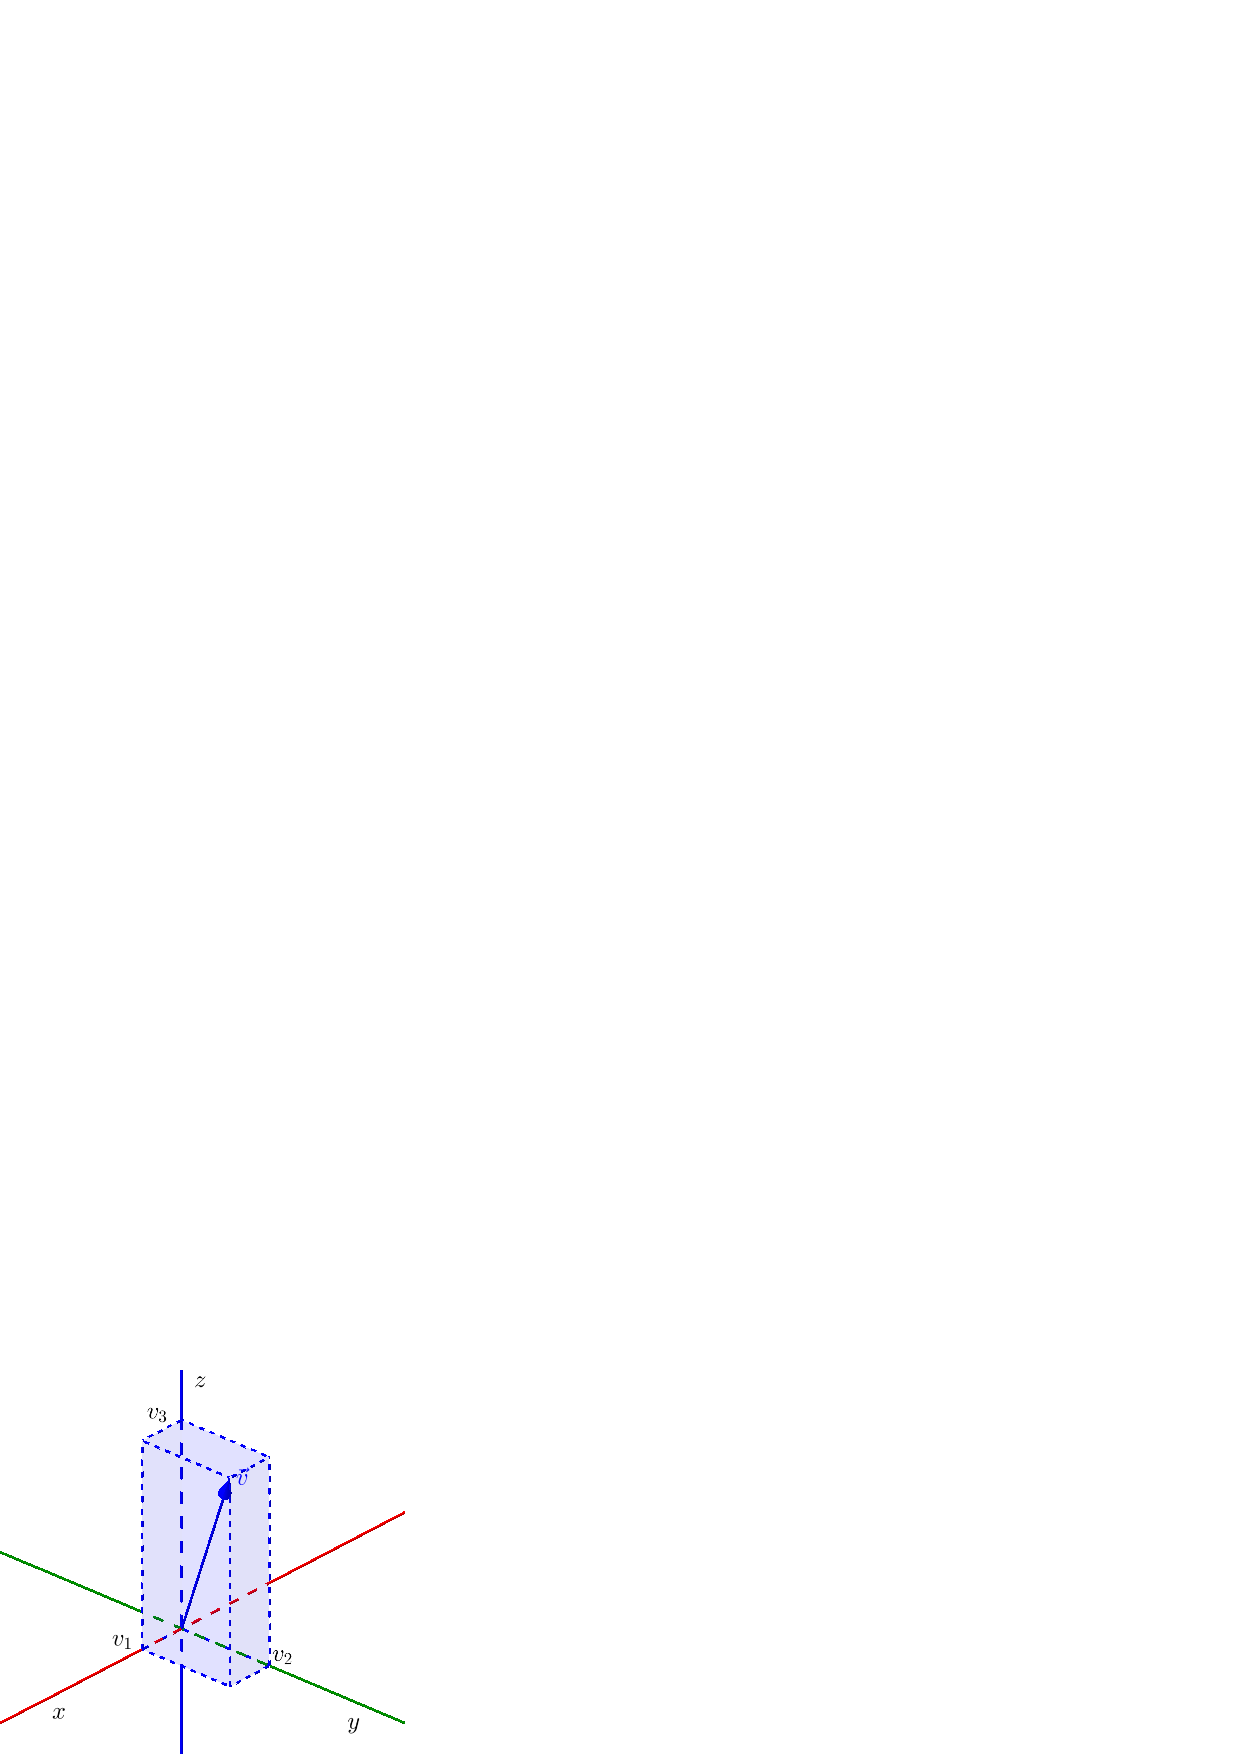
\includegraphics[width=0.2\linewidth]{semana02-coord.png}
\end{center}
\end{figure}

No livro ``�lgebra Linear e suas Aplica��es'', de David Lay, vetores s�o representados por letras em negrito. Nestas notas, utilizamos uma setinha em cima da letra para indicar um vetor.

O conjunto de todos os vetores com tr�s componentes como acima � chamado de $\bR^3$ (leia-se ``erre tr�s''). Em coordenadas, se tivermos
\[
\vec{v} =
\left[
  \begin{array}{c}
    v_1 \\
    v_2 \\
    v_3 \\
  \end{array}
\right]  \quad  \text{e} \quad
\vec{w} =
\left[
  \begin{array}{c}
    w_1 \\
    w_2 \\
    w_3 \\
  \end{array}
\right],
\] podemos definir a \textbf{soma de vetores} componente a componente:
\[
\vec{v} + \vec{w} :=
\left[
  \begin{array}{c}
    v_1 + w_1 \\
    v_2 + w_2 \\
    v_3 + w_3 \\
  \end{array}
\right].
\] Geometricamente, isto pode ser interpretado como segue:
\begin{figure}[h!]
\begin{center}
\includegraphics[width=0.3\linewidth]{semana02-soma.png}
\end{center}
\end{figure}

A \textbf{multiplica��o} do vetor $\vec{v}$ \textbf{por escalar} $k \in \bR$ � definida como:
\[
k \vec{v} :=
\left[
  \begin{array}{c}
    k v_1 \\
    k v_2 \\
    k v_3 \\
  \end{array}
\right].
\] Geometricamente,
\begin{figure}[h!]
\begin{center}
\includegraphics[width=0.3\linewidth]{semana02-escalar.png}
\end{center}
\end{figure}



Estas considera��es que fizemos tamb�m s�o v�lidas para outro n�mero de componentes, com a poss�vel perda de visualiza��o geom�trica, no caso de quatro ou mais componentes.

Mais geralmente, um vetor $\vec{v}$ do conjunto $\bR^n$ pode ser pensado como um objeto com $n$ componentes:
\[
\vec{v} =
\left[
  \begin{array}{c}
    v_1 \\
    v_2 \\
   \vdots \\
    v_{n-1} \\
    v_n \\
  \end{array}
\right]
= v_1 \vec{e}_1 + v_2 \vec{e}_2 + \cdots + v_{n-1} \vec{e}_{n-1} + v_{n} \vec{e}_{n},
\] onde
\[
\vec{e}_1 =
\left[
  \begin{array}{c}
    1 \\
    0 \\
  \vdots \\
    0 \\
    0 \\
  \end{array}
\right], \quad
\vec{e}_2 =
\left[
  \begin{array}{c}
    0 \\
    1 \\
    0 \\
  \vdots \\
    0 \\
  \end{array}
\right], \quad  \cdots,
\vec{e}_{n-1} =
\left[
  \begin{array}{c}
    0 \\
    0 \\
  \vdots \\
    1 \\
    0 \\
  \end{array}
\right], \quad
\vec{e}_n =
\left[
  \begin{array}{c}
    0 \\
    0 \\
  \vdots \\
    0 \\
    1 \\
  \end{array}
\right].
\] A soma de vetores � dada em coordenadas por:
\[
\vec{v} + \vec{w} :=
\left[
  \begin{array}{c}
    v_1 + w_1 \\
    v_2 + w_2 \\
    \vdots \\
    v_{n-1} + w_{n-1} \\
    v_n + w_n \\
  \end{array}
\right].
\] A multiplica��o por escalar por:
\[
k \vec{v} :=
\left[
  \begin{array}{c}
    k v_1 \\
    k v_2 \\
    \vdots \\
    k v_{n-1} \\
    k v_n \\
  \end{array}
\right].
\]



\subsection{Representa��o matricial para sistemas Lineares}

Na linguagem da se��o anterior, n�s dizemos que dois vetores s�o iguais quando todas as suas componentes s�o iguais. Desta forma, podemos interpretar as equa��es de um sistema linear
\begin{equation*}
  \left\{
    \begin{array}{rcl}
      x+3y&=&1 \\
      2x-y&=&-2
    \end{array}
  \right.
\end{equation*} como uma igualdade entre vetores de $\bR^2$, isto �, de vetores com duas componentes:
\begin{equation*}
  \left[
    \begin{array}{c}
      x+3y \\
      2x-y
    \end{array}
  \right] =
    \left[
    \begin{array}{c}
      -1 \\
      2
    \end{array}
  \right].
\end{equation*} Al�m disso, desta forma surge o \textbf{produto de uma matriz por um vetor}:
\begin{equation*}
  \left[
    \begin{array}{cc}
      1 & 3 \\
      2 & -1 \\
    \end{array}
  \right]
  \left[
    \begin{array}{c}
      x \\
      y
    \end{array}
  \right] =
    \left[
    \begin{array}{c}
      -1 \\
      2
    \end{array}
  \right],
\end{equation*} definido de modo que as duas �ltimas equa��es acima signifiquem a mesma coisa. Esta �ltima nota��o � conhecida como a \textbf{forma matricial} do sistema linear.




\begin{example}
O sistema, que j� apareceu nas notas da semana anterior
\[
\left\{
  \begin{array}{ll}
    x_1 + 2x_2 + x_3 = 12 \\
    x_1 -3x_2 + 5x_3 = 1 \\
    2x_1 - x_2 + 3x_3 = 10
  \end{array}
\right.
\] pode ser representado matricialmente por
\[
\left[
  \begin{array}{ccc}
    1 &  2 & 1  \\
    1 & -3 & 5  \\
    2 & -1 & 3  \\
  \end{array}
\right]
\left[
  \begin{array}{c}
    x_1   \\
    x_2  \\
    x_3 \\
  \end{array}
\right] =
\left[
  \begin{array}{c}
    12   \\
    1  \\
    10   \\
  \end{array}
\right].
\] De forma mais sucinta,
\[
\boxed{A \vec{x} = \vec{b}}
\] onde
\[
A = \left[
  \begin{array}{ccc}
    1 &  2 & 1  \\
    1 & -3 & 5  \\
    2 & -1 & 3  \\
  \end{array}
\right], \quad
\vec{x} = \left[
  \begin{array}{c}
    x_1   \\
    x_2  \\
    x_3 \\
  \end{array}
\right], \ \text{ e } \
\vec{b} = \left[
  \begin{array}{c}
    12   \\
    1  \\
    10   \\
  \end{array}
\right].
\]
\end{example}


Mais geralmente, uma matriz do tipo $m\times n$ (leia-se ``$m$ por $n$'') � uma matriz com $m$ linhas e $n$ colunas:
\[
A = \left(a_{ij}\right) =
\begin{bmatrix}
a_{11}&a_{12}&\cdots &a_{1n}\\
a_{21}&a_{22}&\cdots &a_{2n}\\
\vdots &\vdots &\ddots &\vdots \\
a_{m1}&a_{m2}&\cdots &a_{mn}
\end{bmatrix}
\] e pode estar associada a um sistema com $m$ equa��es e $n$ vari�veis, j� que o produto
\[
\left[
  \begin{array}{cccc}
  a_{11}&a_{12}&\cdots &a_{1n}\\
  a_{21}&a_{22}&\cdots &a_{2n}\\
  \vdots &\vdots &\ddots &\vdots \\
  a_{m1}&a_{m2}&\cdots &a_{mn} \\
\end{array}
\right]
\left[
  \begin{array}{c}
    x_1 \\
    x_2 \\
    \vdots \\
    x_n \\
  \end{array}
\right] =
\left[
  \begin{array}{c}
    b_1 \\
    b_2 \\
    \vdots \\
    b_m \\
  \end{array}
\right],
\] quando visto componente a componente, representa:
\[
\left\{
  \begin{array}{cc}
  a_{11} x_1 + a_{12} x_2 + \cdots + a_{1n} x_n =  b_1 \\
  a_{21} x_1 + a_{22} x_2 + \cdots + a_{2n} x_n =  b_2 \\
    \vdots \\
  a_{m1} x_1 + a_{m2} x_2 + \cdots + a_{mn} x_n =  b_m \\
\end{array}
\right.
\]





\section{Combina��es lineares de vetores}

Uma \textbf{combina��o linear} dos vetores $\vec{v}_1, \vec{v}_2, \dots, \vec{v}_k$ � um vetor da forma:
\[
\vec{v} = x_1 \vec{v}_1 + x_2 \vec{v}_2 + \cdots + x_k \vec{v}_k = \sum_{i=1}^k x_i \vec{v}_i,
\] onde $x_1, x_2, \dots, x_k$ s�o n�meros reais. Em outras palavras, uma combina��o linear � uma soma de m�ltiplos dos vetores $\vec{v}_1, \vec{v}_2, \dots, \vec{v}_k$.


\begin{example}
Para os vetores
\[
\vec{v}_1 = \left[
  \begin{array}{c}
    1 \\
    -1 \\
  \end{array}
\right] \quad \text{e} \quad
\vec{v}_2 = \left[
  \begin{array}{c}
    1 \\
    3 \\
  \end{array}
\right],
\] algumas combina��es lineares s�o:
\begin{itemize}
  \item $\vec{v}_1 + \vec{v}_2 =
  \left[
  \begin{array}{c}
    1 \\
    -1 \\
  \end{array}
\right] +
\left[
  \begin{array}{c}
    1 \\
    3 \\
  \end{array}
\right] =
\left[
  \begin{array}{c}
    2 \\
    2 \\
  \end{array}
\right];$
  \item $ 4 \vec{v}_1 = 4 \vec{v}_1 + 0 \vec{v}_2 =
  4 \left[
  \begin{array}{c}
    1 \\
    -1 \\
  \end{array}
\right] =
\left[
  \begin{array}{c}
    4 \\
    -4 \\
  \end{array}
\right];$
  \item $ \vec{v}_2 = 0\vec{v}_1 + 1\vec{v}_2 =
   \left[
  \begin{array}{c}
    1 \\
    3 \\
  \end{array}
\right];$
  \item $0\vec{v}_1 + 0 \vec{v}_2 =
  \left[
  \begin{array}{c}
    0 \\
    0 \\
  \end{array}
\right] = \vec{0}.$
\end{itemize} \textbf{Geometricamente}, qualquer vetor do plano pode ser representado como combina��o linear de vetores que n�o s�o colineares.

Vamos ilustrar este fato na figura abaixo.
\begin{figure}[h!]
\begin{center}
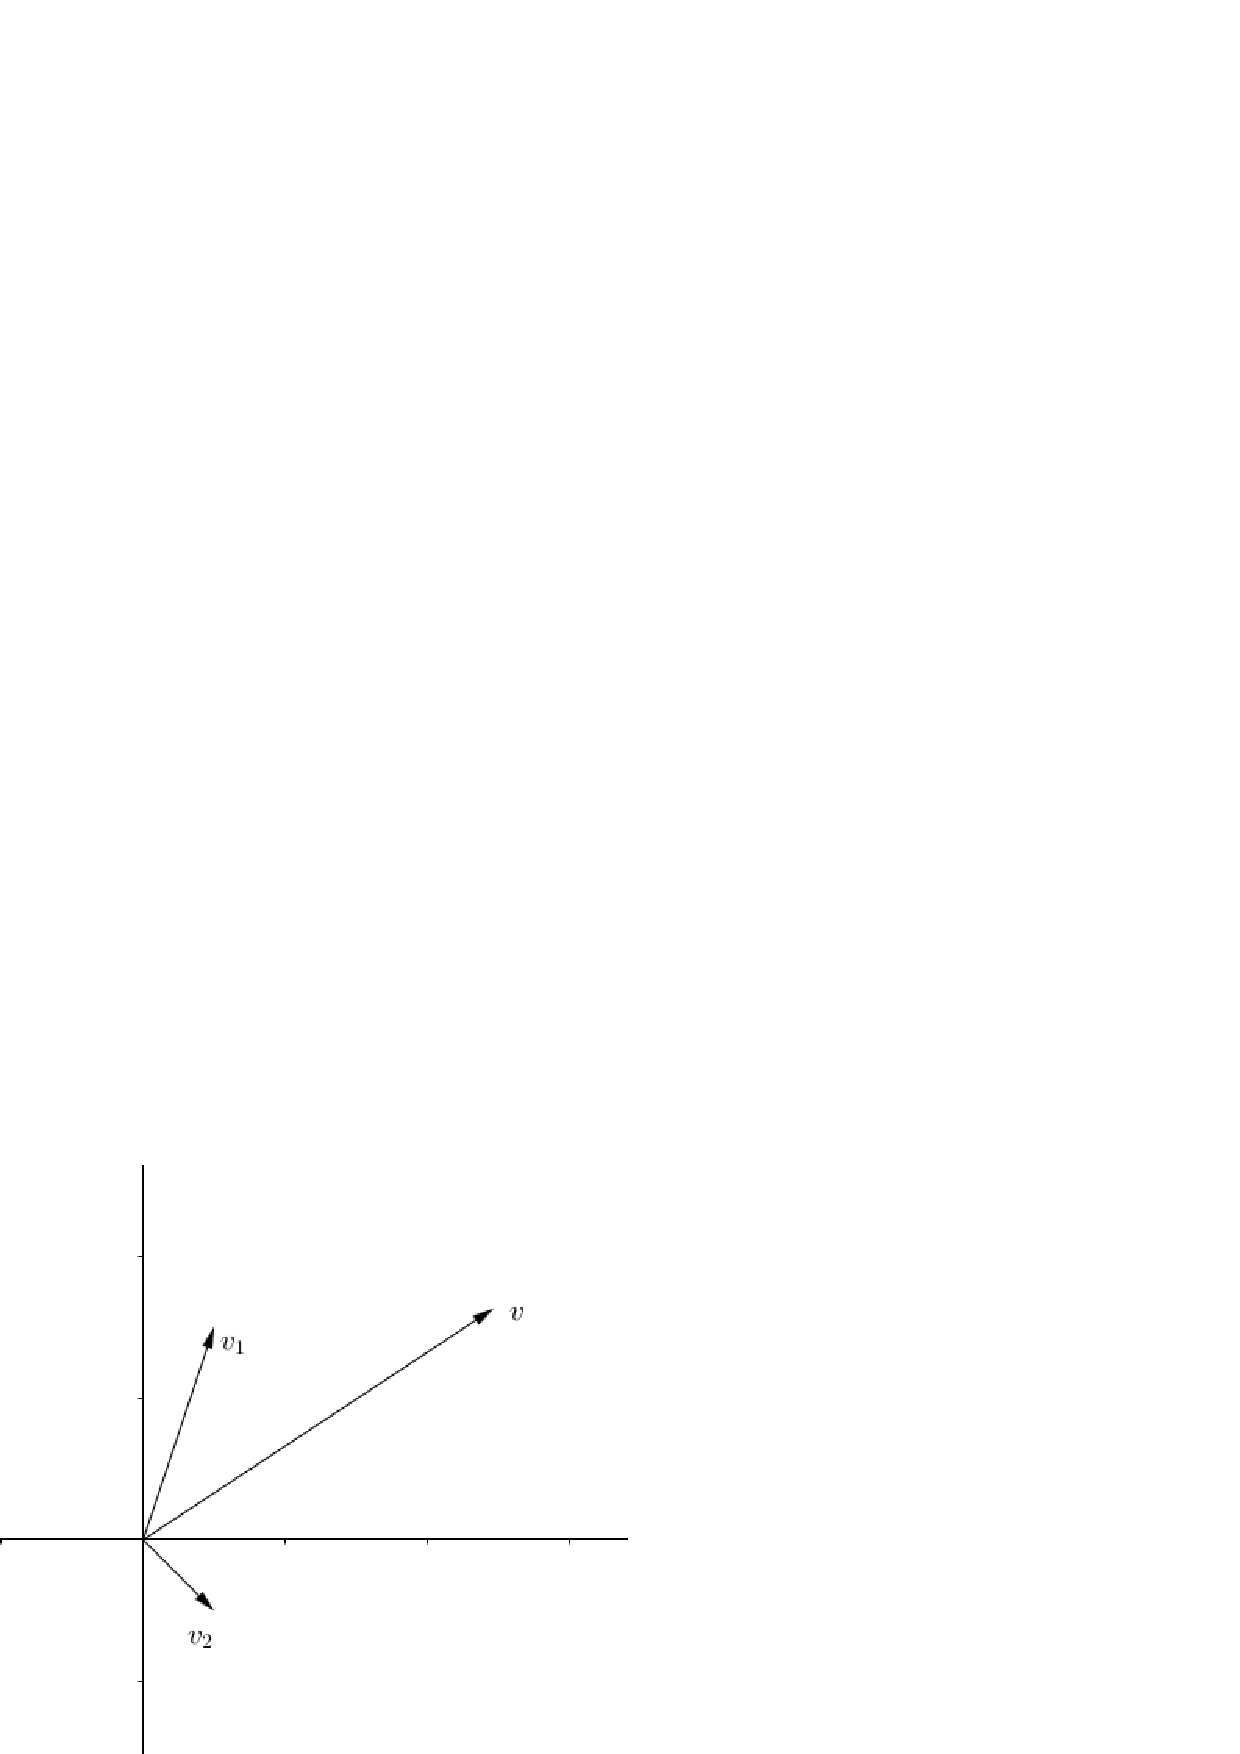
\includegraphics[width=0.4\linewidth]{semana02-comblinear1.png}
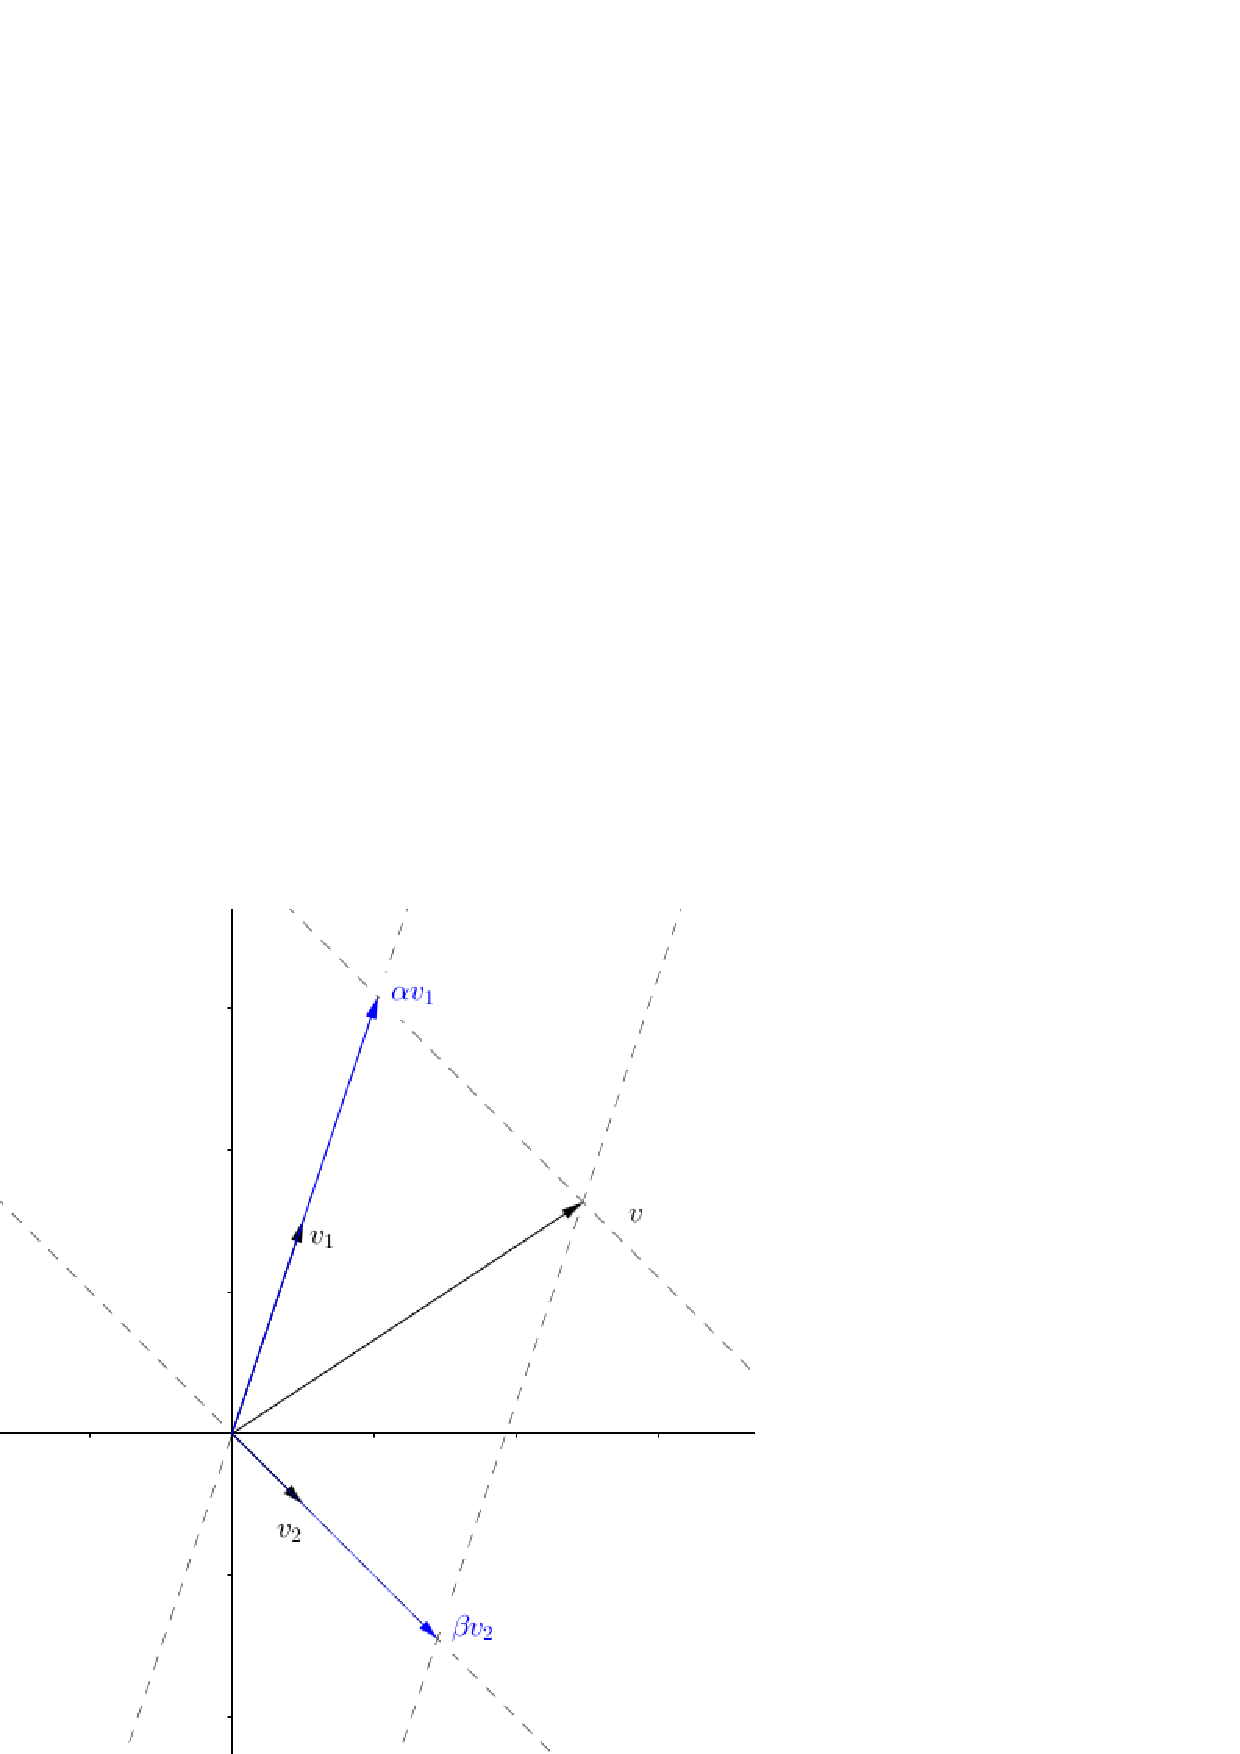
\includegraphics[width=0.4\linewidth]{semana02-comblinear3.png}
\end{center}
\end{figure}
Por exemplo, para representar o vetor $\vec{v}$ como combina��o linear de $\vec{v}_1$ e $\vec{v}_2$, podemos tra�ar retas paralelas aos vetores, passando pela origem e pela extremidade do vetor $\vec{v}$, como na figura da direita. Assim, pela interpreta��o geom�trica da soma de vetores (ver in�cio das notas), sabemos que $\vec{v}$ � a soma dos vetores em azul. Mas estes, por constru��o, s�o colineares aos vetores iniciais e logo m�ltiplos destes. Concluimos que
\[
\vec{v} = \alpha \vec{v}_1 + \beta \vec{v}_2,
\] isto �, $\vec{v}$ � uma combina��o linear de $\vec{v}_1$ e $\vec{v}_2$. $\ \lhd$
\end{example}



De forma mais geral, n�s dizemos que um vetor $\vec{v} \in \bR^m$ � combina��o linear dos $k$ vetores $\vec{v}_1, \vec{v}_2, \dots, \vec{v}_k  \in \bR^m$ quando conseguirmos encontrar n�meros reais $x_1, x_2, \dots, x_k$ tais que
\[
x_1 \vec{v}_1 + x_2 \vec{v}_2 + \dots + x_k \vec{v}_k = \vec{v}.
\] N�s vamos nos referir a este tipo de equa��o por \textbf{equa��o vetorial}. Para decidir se um vetor � combina��o linear de outros, devemos decidir se existem estes n�meros reais $x_1, x_2, \dots, x_k$. Escrevendo em coordenadas:
\[
\vec{v}_1 =
\left[
  \begin{array}{c}
    v_{11} \\
    v_{21} \\
    v_{31} \\
    \vdots \\
    v_{m1} \\
  \end{array}
\right], \
\vec{v}_2 =
\left[
  \begin{array}{c}
    v_{12} \\
    v_{22} \\
    v_{32} \\
    \vdots \\
    v_{m2} \\
  \end{array}
\right], \
\vec{v}_3 =
\left[
  \begin{array}{c}
    v_{13} \\
    v_{23} \\
    v_{33} \\
    \vdots \\
    v_{m3} \\
  \end{array}
\right], \ \cdots, \
\vec{v}_k =
\left[
  \begin{array}{c}
    v_{1k} \\
    v_{2k} \\
    v_{3k} \\
    \vdots \\
    v_{mk} \\
  \end{array}
\right], \
\vec{v} =
\left[
  \begin{array}{c}
    b_{1} \\
    b_{2} \\
    b_{3} \\
    \vdots \\
    b_{m} \\
  \end{array}
\right],
\] vemos que encontrar os coeficientes da combina��o linear, caso estes existam, equivale a resolver a equa��o vetorial
\[
x_1 \left[
  \begin{array}{c}
    v_{11} \\
    v_{21} \\
    v_{31} \\
    \vdots \\
    v_{m1} \\
  \end{array}
\right] + x_2
\left[
  \begin{array}{c}
    v_{12} \\
    v_{22} \\
    v_{32} \\
    \vdots \\
    v_{m2} \\
  \end{array}
\right] + x_3
\left[
  \begin{array}{c}
    v_{13} \\
    v_{23} \\
    v_{33} \\
    \vdots \\
    v_{m3} \\
  \end{array}
\right] + \cdots + x_k
\left[
  \begin{array}{c}
    v_{1k} \\
    v_{2k} \\
    v_{3k} \\
    \vdots \\
    v_{mk} \\
  \end{array}
\right] =
\left[
  \begin{array}{c}
    b_{1} \\
    b_{2} \\
    b_{3} \\
    \vdots \\
    b_{m} \\
  \end{array}
\right],
\] que, por sua vez, � equivalente a
\[
\left[
  \begin{array}{c}
   v_{11} x_1 + v_{12} x_2 + v_{13} x_3 + \cdots + v_{1k} x_k  \\
   v_{21} x_1 + v_{22} x_2 + v_{23} x_3 + \cdots + v_{2k} x_k  \\
   v_{31} x_1 + v_{32} x_2 + v_{33} x_3 + \cdots + v_{3k} x_k  \\
   \vdots  \\
   v_{m1} x_1 + v_{m2} x_2 + v_{m3} x_3 + \cdots + v_{mk} x_k  \\
  \end{array}
\right] =
\left[
  \begin{array}{c}
    b_{1} \\
    b_{2} \\
    b_{3} \\
    \vdots \\
    b_{m} \\
  \end{array}
\right].
\] Mas isto � resolver um sistema linear! Portanto novo conceito est� intimamente relacionado com tudo o que j� t�nhamos visto antes.


O \textbf{espa�o gerado} por todas as combina��es lineares dos vetores $\vec{v}_1, \vec{v}_2, \dots, \vec{v}_k$ � denotado por $\Span \{ \vec{v}_1, \vec{v}_2, \dots, \vec{v}_k \}$.

\begin{itemize}
\item Vimos que o conjunto gerado pelos dois vetores do exemplo anterior � o plano inteiro, isto �, $\Span \{ \vec{v}_1, \vec{v}_2 \} = \bR^2$.
\item Nota que o vetor nulo sempre pertence ao espa�o gerado, assim como todos os vetores $\vec{v}_1, \vec{v}_2, \dots, \vec{v}_k$.
\item O conjunto gerado por apenas um vetor n�o nulo representa uma reta.
\end{itemize}



\section{Sistemas lineares e combina��es lineares das colunas}

A associa��o feita acima pode ser resumida como:
\[
\boxed{\begin{split}
\text{Resolver o sistema linear $A \vec{x} = \vec{b}$ equivale a decidir se o} \\ \text{vetor $\vec{b}$ � uma combina��o linear das colunas de $A$.}
\end{split}}
\] ou ainda
\[
\boxed{\begin{split}
\text{Resolver o sistema linear $A \vec{x} = \vec{b}$ equivale a decidir se o} \\ \text{vetor $\vec{b}$ pertence ao espa�o gerado pelas colunas de $A$.}
\end{split}}
\] Desta forma, tudo o que j� vimos sobre exist�ncia de solu��es para sistemas lineares pode ser ``traduzido'' para o contexto de combina��es lineares e espa�os gerados (fa�a as tradu��es!).


\end{document} 
%Este trabalho está licenciado sob a Licença Creative Commons Atribuição-CompartilhaIgual 3.0 Não Adaptada. Para ver uma cópia desta licença, visite http://creativecommons.org/licenses/by-sa/3.0/ ou envie uma carta para Creative Commons, PO Box 1866, Mountain View, CA 94042, USA.

\documentclass[../livro.tex]{subfiles} 


%define o diretório principal
\providecommand{\dir}{..}

%%%%%%%%%%%%%%%%%%%%%%%%%%%%%%%%%%%%%%%%%%%%%
%%%%%%%%%%%%INICIO DO DOCUMENTO%%%%%%%%%%%%%%
%%%%%%%%%%%%%%%%%%%%%%%%%%%%%%%%%%%%%%%%%%%%%

\begin{document}

\chapter{Semana 3}

\section{Dependência e independência linear}

Nós vimos, por definição, que um vetor $\vec{v} \in \mathbb{R}^m$ é combinação linear dos $k$ vetores $\vec{v}_1, \vec{v}_2, \dots, \vec{v}_k  \in \mathbb{R}^m$ quando conseguirmos encontrar números reais $x_1, x_2, \dots, x_k$ tais que
\begin{equation}
x_1 \vec{v}_1 + x_2 \vec{v}_2 + \cdots + x_k \vec{v}_k = \vec{v}.
\end{equation} Vimos também que para decidir se um vetor é combinação linear de outros, devemos verificar se existem estes números reais $x_1, x_2, \dots, x_k$. Em coordenadas, isto é equivalente a resolver o sistema linear:
\begin{equation}
\left[
  \begin{array}{ccccc}
   v_{11} & v_{12} & v_{13} & \cdots & v_{1k}  \\
   v_{21} & v_{22} & v_{23} & \cdots & v_{2k}  \\
   v_{31} & v_{32} & v_{33} & \cdots & v_{3k}  \\
   \vdots & \vdots & \vdots &        & \vdots  \\
   v_{m1} & v_{m2} & v_{m3} & \cdots & v_{mk}  
  \end{array}
\right] \left[
  \begin{array}{c}
    x_{1} \\
    x_{2} \\
    x_{3} \\
    \vdots \\
    x_{k} 
  \end{array}
\right] =
\left[
  \begin{array}{c}
    b_{1} \\
    b_{2} \\
    b_{3} \\
    \vdots \\
    b_{k} 
  \end{array}
\right].
\end{equation}

Agora, dizemos que os vetores $\vec{v}_1, \vec{v}_2, \dots, \vec{v}_k  \in \mathbb{R}^m$ são \textbf{linearmente independentes (LI)} se nenhum dos vetores puder ser escrito combinação linear dos demais. Uma forma de escrever isto matematicamente é a seguinte:
\begin{equation}
\boxed{\text{Se } x_1 \vec{v}_1 + x_2 \vec{v}_2 + \cdots + x_k \vec{v}_k = \vec{0}, \text{ então } x_1 = x_2 = \cdots = x_k = 0.}
\end{equation} De fato, imaginem que pelo menos um dos coeficientes acima fosse diferente de zero, digamos $x_2 \neq 0$. Daí podemos dividir por $x_2$ e conseguiríamos escrever o vetor $\vec{v}_2$ como combinação linear dos demais:
\begin{equation}
\vec{v}_2 = - \frac{x_1}{x_2} \, \vec{v}_1 - \frac{x_3}{x_2} \, \vec{v}_3 - \cdots - \frac{x_k}{x_2} \, \vec{v}_k.
\end{equation} Se os vetores $\vec{v}_1, \vec{v}_2, \dots, \vec{v}_k  \in \mathbb{R}^m$ não forem linearmente independentes, então nós dizemos que eles são \textbf{linearmente dependentes (LD)}.

\begin{example}\label{exp:1}
Vamos verificar se os vetores
\begin{equation}
\left[
  \begin{array}{c}
    1 \\
    0 \\
    0 
  \end{array}
\right], \quad
\left[
  \begin{array}{c}
    1 \\
    1 \\
    0 
  \end{array}
\right], \quad
\left[
  \begin{array}{c}
    1 \\
    1 \\
    1 
  \end{array}
\right]
\end{equation} são LI ou LD.

Para verificar se são LI, nós devemos considerar a equação vetorial
\begin{equation}
x_1 \left[
  \begin{array}{c}
    1 \\
    0 \\
    0 
  \end{array}
\right] +
x_2\left[
  \begin{array}{c}
    1 \\
    1 \\
    0 
  \end{array}
\right] +
x_3\left[
  \begin{array}{c}
    1 \\
    1 \\
    1 
  \end{array}
\right] = \vec{0} =
\left[
  \begin{array}{c}
    0 \\
    0 \\
    0 
  \end{array}
\right].
\end{equation} Como a equação é homogênea, temos pelo menos a solução trivial: $x_1 = 0$, $x_2=0$ e $x_3 = 0$. Se esta for a única solução, então os vetores são LI. Se existir alguma outra solução que não seja a trivial, então os vetores são LD.

Resolver a equação vetorial equivale a resolver o sistema linear
\begin{equation}
\left[
  \begin{array}{ccc}
    1 & 1 & 1 \\
    0 & 1 & 1 \\
    0 & 0 & 1 
  \end{array}
\right]
\left[
  \begin{array}{c}
    x_1 \\
    x_2 \\
    x_3 
  \end{array}
\right] =
\left[
  \begin{array}{c}
    0 \\
    0 \\
    0 
  \end{array}
\right]
\end{equation} É fácil de ver que a única solução deste sistema é a trivial e, portanto, os vetores são LI. Se este sistema não fosse fácil de resolver, deveríamos começar a resolvê-lo por escalonamento, como de costume. $\ \lhd$
\end{example}

\begin{example}\label{exp:2}
Analisamos agora os vetores
\begin{equation}
\left[
  \begin{array}{c}
    1 \\
    0 \\
    1 
  \end{array}
\right], \quad
\left[
  \begin{array}{c}
    1 \\
    1 \\
    0 
  \end{array}
\right], \quad
\left[
  \begin{array}{c}
    1 \\
    1 \\
    1 
  \end{array}
\right], \quad
\left[
  \begin{array}{c}
    -1 \\
    2 \\
    1 
  \end{array}
\right].
\end{equation} Como no exemplo anterior, para verificar se são LI, nós devemos considerar a equação vetorial
\begin{equation}
x_1 \left[
  \begin{array}{c}
    1 \\
    0 \\
    0 
  \end{array}
\right] +
x_2\left[
  \begin{array}{c}
    1 \\
    1 \\
    0 
  \end{array}
\right] +
x_3\left[
  \begin{array}{c}
    1 \\
    1 \\
    1 
  \end{array}
\right]+
x_4\left[
  \begin{array}{c}
    -1 \\
    2 \\
    1 
  \end{array}
\right] =
\left[
  \begin{array}{c}
    0 \\
    0 \\
    0 
  \end{array}
\right].
\end{equation} Como a equação é homogênea, temos pelo menos a solução trivial: $x_1 = 0$, $x_2=0$ e $x_3 = 0$. Se esta for a única solução, então os vetores são LI. Se existir alguma outra solução que não seja a trivial, então os vetores são LD.

Resolver a equação vetorial equivale a resolver o sistema linear
\begin{equation}
\left[
  \begin{array}{cccc}
    1 & 1 & 1 & -1 \\
    0 & 1 & 1 & 2  \\
    1 & 0 & 1 & 1 
  \end{array}
\right]
\left[
  \begin{array}{c}
    x_1 \\
    x_2 \\
    x_3 \\
    x_4 
  \end{array}
\right] =
\left[
  \begin{array}{c}
    0 \\
    0 \\
    0 
  \end{array}
\right].
\end{equation} Em um sistema com mais variáveis do que equações, podemos não ter soluções (no caso de alguma linha inconsistente) ou podemos ter infinitas soluções (no caso de haver variáveis livres). Não é possível ter unicidade. Como já sabemos que em um sistema homogêneo, sempre temos pelo menos a solução trivial $x_1 = 0$, $x_2=0$, $x_3=0$ e $x_4 = 0$, podemos concluir que existem infinitas soluções. Logo, o conjunto de vetores é LD.
\end{example}

O argumento que utilizamos no Exemplo \ref{exp:2} acima é geral e se aplica em várias situações. Temos
\begin{equation}
\boxed{\text{Se $k>m$, então os vetores } \vec{v}_1, \vec{v}_2, \dots, \vec{v}_k  \in \mathbb{R}^m \text{ são necessariamente LD.}}
\end{equation} Desta forma, não existem quatro vetores LI em $\mathbb{R}^3$. Não conseguiríamos encontrar sete vetores LI em $\mathbb{R}^5$ e assim por diante.


Façamos agora algumas observações gerais sobre independência linear:
\begin{itemize}
  \item O vetor nulo, mesmo que sozinho, é LD. Se $\vec{v} = \vec{0}$ estiver em um conjunto de vetores, este conjunto será automaticamente LD.
  \item Ao considerarmos apenas dois vetores $\vec{u}$ e $\vec{v}$, dizer que estes vetores são LD significa que eles são múltiplos um do outro e, portanto, colineares.
  \item Veremos mais adiante no curso que a dimensão do espaço gerado por vetores linearmente independentes é exatamente o número de vetores. Desta maneira, concluiremos, por exemplo, que o conjunto gerado por dois vetores do espaço tridimensional é um espaço linear de dimensão dois: um plano.
\end{itemize}

\subsection*{Exercícios resolvidos}

\construirExeresol

\subsection*{Exercícios}

\construirExer


\section{Independência linear e sistemas lineares}

Na última semana (capítulo anterior), vimos que resolver o sistema linear $A \vec{x} = \vec{b}$ equivale a decidir se o vetor $\vec{b}$ é uma combinação linear das colunas de $A$. Na seção anterior, introduzimos a questão de decidir se os vetores $\vec{v}_1, \vec{v}_2, \dots, \vec{v}_k$ são LI ou LD. Isto, consequentemente\footnote{Lembra que uma equação vetorial pode ser reescrita como uma equação matricial!}, equivale a decidir se existe solução não trivial para o sistema linear homogêneo
\begin{equation}
A \vec{x} = \vec{0},
\end{equation} onde a matriz $A$ é formada com os vetores $\vec{v}_1, \vec{v}_2, \dots, \vec{v}_k$ como colunas.

\begin{example}
Naturalmente, podemos traduzir os exemplos da seção anterior desta forma. Ou seja no Exemplo \ref{exp:1}, temos que a matriz
\begin{equation}
A = \left[
  \begin{array}{ccc}
    1 & 1 & 1  \\
    0 & 1 & 1   \\
    1 & 0 & 1 
    \end{array}
\right]
\end{equation} tem as colunas linearmente independentes (LI). Por outro lado, as colunas da matriz
\begin{equation}
B = \left[
  \begin{array}{cccc}
    1 & 1 & 1 & -1 \\
    0 & 1 & 1 & 2  \\
    1 & 0 & 1 & 1 
  \end{array}
\right]
\end{equation} do Exemplo \ref{exp:2} são linearmente dependentes (LD). $\ \lhd$
\end{example}

Podemos pensar ainda de outra forma. Considere uma matriz $A$ de ordem $m\times n.$ Para decidir se as colunas de $A$ são LI, devemos procurar por soluções não triviais do sistema linear cuja matriz associada é $A$. Ao resolver um \textbf{sistema homogêneo} por escalonamento, sabemos que
\begin{itemize}
  \item Se existirem mais colunas do que linhas ($i.e. \ m<n$), então as colunas de $A$ são necessariamente LD.
  \item Se existirem mais linhas do que colunas ($i.e. \ m>n$), procedemos por escalonamento. Se todas as colunas da matriz $A$ possuirem posição de pivô, então as colunas são LI (pois daí a única solução do sistema homogêneo é a trivial). 
  \item No caso de alguma coluna não possuir posição de pivô, o sistema homogêneo possui pelo menos uma variável livre; logo, as colunas de $A$ são LD.
\end{itemize}

\begin{example}
Decidir se as colunas de $A$ são LI:
\begin{equation}
A = \left[
\begin{array}{rrrr}
   2&1&-1&8\\
   -3&-1&2&-11\\
   6&2&-4&22\\
   -2&1&2&-3
\end{array}
\right].
\end{equation} Como as colunas de $A$ são quatro vetores de $\mathbb{R}^4$, pode ser que sejam LI (caso tivesse uma coluna a mais, saberíamos automaticamente serem LD). Aplicando o algoritmo de escalonamento, sabemos que
\begin{equation}
A \sim \left[
\begin{array}{cccc}
   2&1&-1&8\\
   0&1&1&2\\
   0&0&-1&1\\
   0&0&0&0
\end{array}
\right].
\end{equation} Notando que a última coluna não possui posição de pivô, concluimos que as colunas de $A$ são LD. Isto pois, neste caso, o sistema linear homogêneo associado, $A \vec{x} = \vec{0}$, cuja matriz aumentada associada é
\begin{equation}
\left[
\begin{array}{cccc|c}
   2&1&-1&8&0\\
   0&1&1&2& 0\\
   0&0&-1&1&0\\
   0&0&0&0&0
\end{array}
\right],
\end{equation} possui uma variável livre (e portanto outras soluções que não a trivial). $\ \lhd$
\end{example}

\subsection*{Exercícios resolvidos}

\construirExeresol

\subsection*{Exercícios}

\construirExer


\section{Transformações lineares}


Uma \textbf{transformação linear} é um tipo especial de função que associa um vetor a outro vetor
\begin{equation}
T: \{ \text{vetores} \} \to \{ \text{vetores} \}
\end{equation} e com a propriedade adicional:
\begin{equation}
T\big( a \vec{u} + b \vec{v} \big) = aT(\vec{u}) + bT(\vec{v}), \quad \text{para todos } a, b \in \mathbb{R} \quad \text{e todos } \vec{u}, \vec{v}.
\end{equation}
Em geral, pensamos em uma transformação linear como ``transformando um vetor em outro'' de forma linear, isto é, satisfazendo a propriedade acima.


\begin{example}
A aplicação $T: \mathbb{R}^3 \to \mathbb{R}^3$ dada por $T(\vec{u}) = 3\vec{u}$ é a transformação linear que transforma um vetor de $\mathbb{R}^3$ no vetor que tem o triplo do comprimento. Utilizamos a própria fórmula da transformada para verificar que a tranformação $T$ é de fato linear:
\begin{equation}
T\big( a \vec{u} + b \vec{v} \big) = 3 ( a \vec{u} + b \vec{v} ) = a \cdot 3 \vec{u} + b \cdot 3 \vec{v} = aT(\vec{u}) + bT(\vec{v}). \lhd
\end{equation}
\end{example}


\begin{example}\label{exp:4}
Também é linear a transformação que faz uma rotação de um ângulo $\pi / 2$. Tente se convencer geometricamente que esta transformação é uma transformação linear. Voltaremos a este exmeplo com mais detalhes na seção seguinte$. \ \lhd$
\end{example}



\begin{example}\label{exp:7}
Consideramos a transformação $T: \mathbb{R}^2 \to \mathbb{R}^3$, que transforma vetores de $\mathbb{R}^2$ em vetores de $\mathbb{R}^3$, dada pela fórmula
\begin{equation}
T(x_1, x_2) = (x_1 - 3 x_2, 3x_1 + 5x_2, -x_1 + x_2).
\end{equation} Nota que, excepcionalmente, estamos representando os vetores como linhas. É comum quando tratamos de transformações lineares. Esta fórmula nos diz, por exemplo, que os vetores
\begin{equation}
\vec{u} =
\left[
  \begin{array}{c}
    1 \\
    -1 \\
  \end{array}
\right] \quad \text{e} \quad 
\vec{v} =
\left[
  \begin{array}{c}
    0 \\
    3 \\
  \end{array}
\right]
\end{equation} são transformados nos vetores
\begin{equation}
T\big(\vec{u}\big) =
\left[
  \begin{array}{c}
    1-3\cdot(-1) \\
    3\cdot 1 + 5\cdot(-1) \\
    -1 + (-1)\\
  \end{array}
\right] =
\left[
  \begin{array}{r}
     4 \\
    -2 \\
    -2 \\
  \end{array}
\right] \quad \text{e} \quad
T\big(\vec{v}\big) =
\left[
  \begin{array}{c}
    0-3\cdot 3 \\
    3\cdot 0 + 5\cdot 3 \\
    -0 + 3 \\
  \end{array}
\right] =
\left[
  \begin{array}{r}
    -9 \\
    15 \\
     3 \\
  \end{array}
\right].\lhd
\end{equation}
\end{example}




\subsection*{Exercícios resolvidos}

\construirExeresol

\subsection*{Exercícios}

\construirExer



\section{Matriz de uma transformação linear}


Voltemos à transformação linear
\begin{equation}
T(x_1, x_2) = (x_1 - 3 x_2, 3x_1 + 5x_2, -x_1 + x_2)
\end{equation} do Exemplo \ref{exp:7}. Lembramos que um vetor qualquer de $\mathbb{R}^2$ pode ser escrito como combinação linear dos vetores
\begin{equation}
\vec{e}_1 =
\left[
  \begin{array}{r}
    1 \\
    0 \\
  \end{array}
\right]\quad \text{e}\quad
\vec{e}_2 =
\left[
  \begin{array}{c}
    0\\
    1\\
  \end{array}
\right].
\end{equation} De fato,
\begin{equation}
\vec{u} =
\left[
  \begin{array}{r}
    x_1 \\
    x_2 \\
  \end{array}
\right] =
x_1 \left[
  \begin{array}{r}
    1 \\
    0 \\
  \end{array}
\right] +
x_2 \left[
  \begin{array}{c}
    0\\
    1\\
  \end{array}
\right] = x_1 \vec{e}_1 + x_2 \vec{e}_2.
\end{equation} Logo, utilizando a propriedade de a transformação ser linear, temos que
\begin{equation}
T( \vec{u} ) = T\big( x_1 \vec{e}_1 + x_2 \vec{e}_2 \big) = x_1 T(\vec{e}_1) + x_2 T(\vec{e}_2).
\end{equation} Calculamos $T(\vec{e}_1)$ e $T(\vec{e}_2)$ pela fórmula dada da transformação linear:
\begin{equation}
T(\vec{e}_1) =
\left[
  \begin{array}{r}
    1 \\
    3 \\
    -1 \\
  \end{array}
\right] \quad \text{e}\quad
T(\vec{e}_2) =
\left[
  \begin{array}{r}
    -3 \\
     5 \\
     1 \\
  \end{array}
\right].
\end{equation} Concluimos que
\begin{equation}
T( \vec{u} ) =
x_1 \left[
  \begin{array}{r}
    1 \\
    3 \\
    -1 \\
  \end{array}
\right] + x_2
\left[
  \begin{array}{r}
    -3 \\
     5 \\
     1 \\
  \end{array}
\right] =
\left[
  \begin{array}{rr}
    1  & -3 \\
    3  & 5  \\
    -1 & 1 \\
  \end{array}
\right]
\left[
  \begin{array}{r}
    x_1 \\
    x_2 \\
  \end{array}
\right].
\end{equation} Desta forma, associamos uma matriz de ordem $3 \times 2$ à transformação linear $T: \mathbb{R}^2 \to \mathbb{R}^3$.

O procedimento que aplicamos acima não é particular do exemplo que analisamos, de modo que é sempre possível associar a uma transformação linear $T: \mathbb{R}^n \to \mathbb{R}^m$ uma matriz $A$ de ordem $m\times n$, chamada \textbf{matriz canônica associada à transformação linear} $T$ ou apenas \textbf{matriz associada} a $T$, cujas colunas são os vetores $T(\vec{e}_1), T(\vec{e}_2), T(\vec{e}_3), \dots, T(\vec{e}_n) \in \mathbb{R}^m$ (e portanto $n$ colunas com $m$ componentes cada).


\begin{example}
A transformação linear $T: \mathbb{R}^3 \to \mathbb{R}^3$, $T(\vec{u}) = 5 \vec{u}$, satisfaz
\begin{equation}
T(\vec{e}_1) =
\left[
  \begin{array}{r}
    5 \\
    0 \\
    0 \\
  \end{array}
\right], \quad
T(\vec{e}_2) =
\left[
  \begin{array}{r}
     0 \\
     5 \\
     0 \\
  \end{array}
\right]  \quad \text{e} \quad
T(\vec{e}_3) =
\left[
  \begin{array}{r}
     0 \\
     0 \\
     5 \\
  \end{array}
\right].
\end{equation} Assim, podemos escrever
\begin{equation}
T(\vec{x}) = \left[
  \begin{array}{rrr}
    5  & 0 & 0 \\
    0  & 5 & 0 \\
    0  & 0 & 5 \\
  \end{array}
\right]
\left[
  \begin{array}{r}
    x_1 \\
    x_2 \\
    x_3 \\
  \end{array}
\right]. \lhd
\end{equation}
\end{example}


\begin{example}\label{exp:rotacao}
O método acima pode também ser aplicado para conseguirmos uma fórmula para transformações lineares como as do Exemplo \ref{exp:4}. Vamos considerar a aplicação $T: \mathbb{R}^2 \to \mathbb{R}^2$ definida por
\begin{equation}
T(\vec{x}) = \text{rotação no sentido anti-horário de $\vec{x}$ por um ângulo } \theta \in (0, 2\pi).
\end{equation} A matriz da transformação linear tem por colunas a imagem por $T$ dos vetores $\vec{e}_1$ e $\vec{e}_2$. Observamos que (ver figura)
\begin{figure}[h!]
\begin{center}
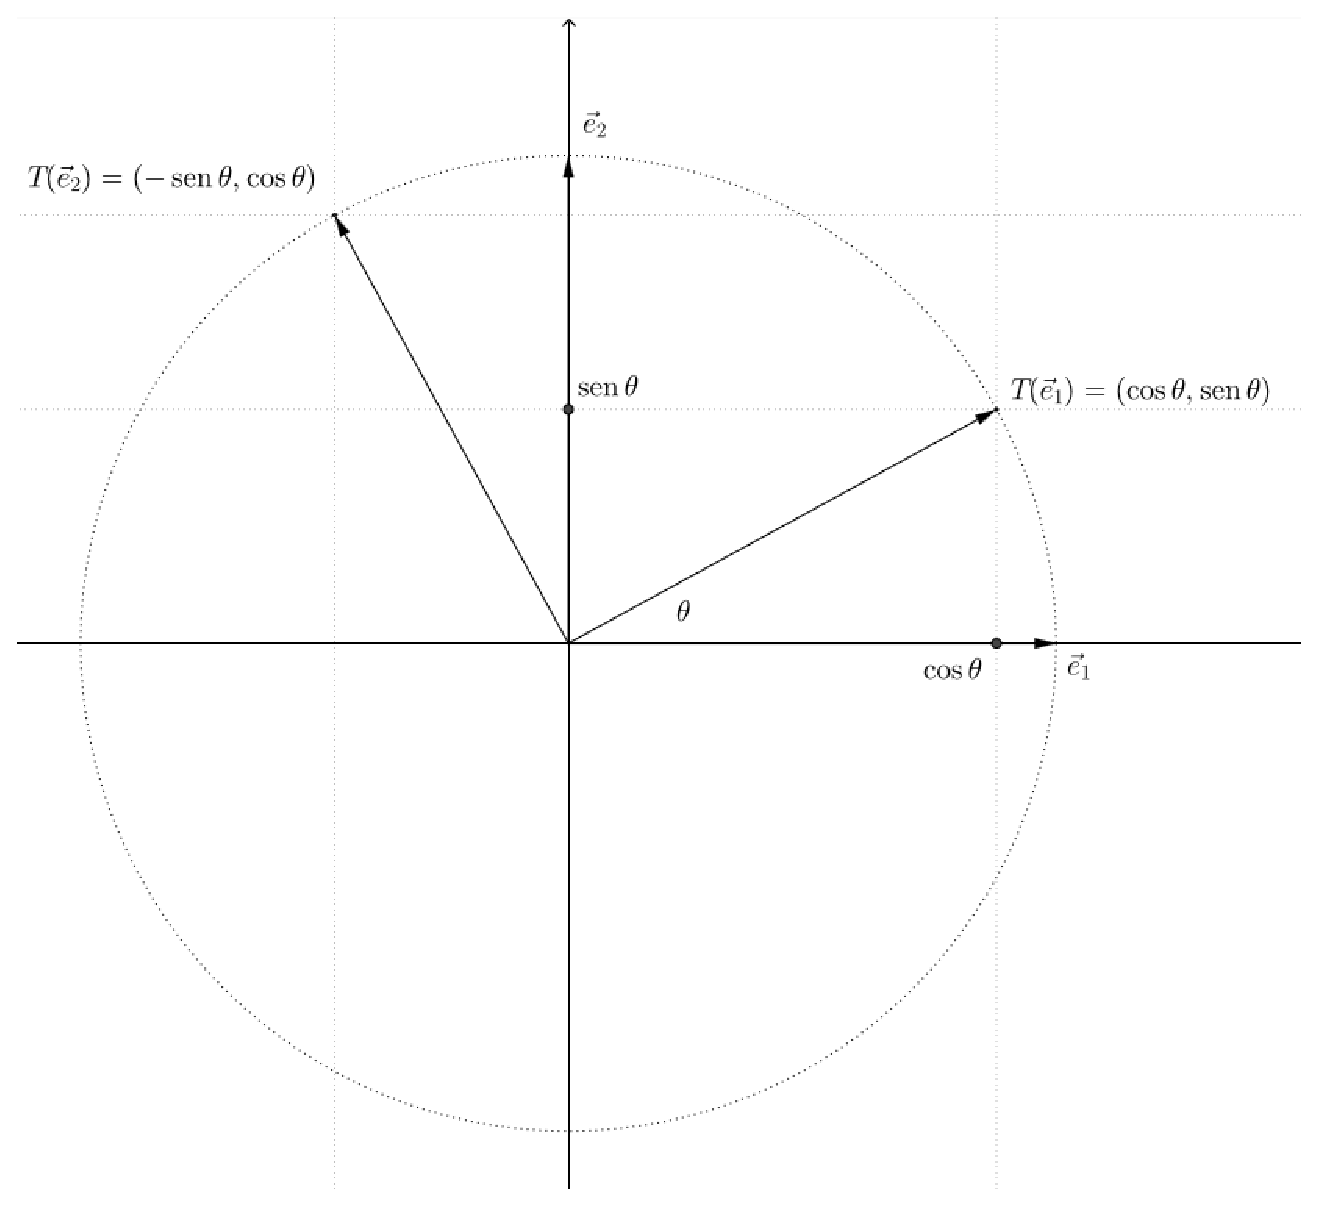
\includegraphics[width=0.8\linewidth]{\dir/Semana03/semana03-rot}
\end{center}
\end{figure}
\begin{equation}
T(\vec{e}_1) =
\left[
  \begin{array}{r}
    \cos \theta \\
    \sen \theta \\
  \end{array}
\right], \quad T(\vec{e}_2) =
\left[
  \begin{array}{r}
    - \sen \theta \\
    \cos \theta \\
  \end{array}
\right].
\end{equation} Logo, concluimos que
\begin{equation}
T(\vec{x}) = \left[
  \begin{array}{rr}
    \cos \theta  & - \sen \theta \\
    \sen \theta  & \cos \theta \\
  \end{array}
\right]
\left[
  \begin{array}{r}
    x_1 \\
    x_2 \\
  \end{array}
\right].
\end{equation}
\end{example}

\subsection*{Exercícios resolvidos}

\construirExeresol

\subsection*{Exercícios}

\construirExer


\section{Transformações injetoras, sobrejetoras e invertíveis}


Como de costume, dada uma função $f: A \to B$, diz-se que $A$ é o domínio de $f$ enquanto $B$ é o contradomínio. A imagem de $f$ é o subconjunto de $B$ que consiste de todos os elementos $y \in B$ tais que $f(x) = y$ ou, intuitivamente, que consiste de ``todos os elementos de $B$ que são atingidos pela função $f$''.

Na hora de decidir se uma função é invertível ou não, duas propriedades são essenciais:
\begin{enumerate}[$1)$]
  \item cada elemento de $B$ ser a imagem de no máximo um elemento de $A$, caso em que $f$ é dita \textbf{injetora} ou \textbf{injetiva};
  \item a imagem de $f$ ser igual ao contradomínio, caso em que $f$ diz-se \textbf{sobrejetora} ou \textbf{sobrejetiva}.
\end{enumerate}

Quando estas duas propriedades são satisfeitas, isto é, quando a função $f$ é injetora e sobrejetora, vale que $f$ é \textbf{invertível}: podemos encontrar uma função $f^{-1} : B \to A$ que satisfaz
\begin{equation}
f^{-1}\big( f (x)\big) = x, \ \text{para todo } x \in A  \quad \text{e} \quad f\big( f^{-1} (y)\big) = y, \ \text{para todo } y \in B.
\end{equation} Ao tentarmos encontrar uma \textbf{função inversa} $f^{-1}$, as propriedades de ser injetora e sobrejetora, aparecem naturalmente.

Estas definições são usuais para funções quaisquer. A partir de agora, vamos analisar quando que transformações lineares são injetoras, sobrejetoras e/ou invertíveis. Vamos ver, em particular, que é bem mais fácil estudar tais propriedades para transformações lineares.

\subsection{Transformações lineares injetoras}

A transformação linear $T: \mathbb{R}^n \to \mathbb{R}^m$ é injetora quando, para $\vec{b} \in \mathbb{R}^m$, a equação
\begin{equation}
T(\vec{x}) = \vec{b}
\end{equation} possuir uma única solução ou nenhuma (no máximo uma -- comparar com a definição acima). Como vimos, existe uma matriz $A$ de ordem $m\times n$ associada à transformação linear $T$, de modo que temos que analisar as soluções de
\begin{equation}
A\vec{x} = \vec{b}.
\end{equation} Recaimos novamente em um sistema linear!

No caso particular em que $\vec{b} = \vec{0}$, o sistema homogêneo $A\vec{x} = \vec{0}$ sempre possui a solução trivial $\vec{x} = \vec{0}$. Neste caso, para que a transformação linear seja injetora devemos verificar que esta é a única solução de $A\vec{x} = \vec{0}$. Na verdade, é possível verificar o seguinte.

% \begin{equation}
% \boxed{\text{$T$ é injetora se, e somente se, $A\vec{x} = \vec{0}$ possui apenas a solução trivial.}}
% \end{equation} Em particular, este caso somente é possível se $n \le m$ (reler observações que seguem o Exemplo 3).


\begin{claim}
  $T$ é injetora se, e somente se, $A\vec{x} = \vec{0}$ possui apenas a solução trivial.\footnote{Em particular, este caso somente é possível se $n \le m$ (reler observações que seguem o Exemplo 3)}
\end{claim}
\begin{proof}[Justificativa da afirmação]
Vamos provar matematicamente que, se soubermos que $A\vec{x} = \vec{0}$ possui apenas a solução trivial, então vale que $A\vec{x} = \vec{b}$ possui no máximo uma solução, para qualquer escolha de vetor $\vec{b}$. Isto, por sua vez, implica que $T$ é injetora. Caso não existam soluções ou caso exista apenas uma, nada há para provar. Suponhamos que então que existem infinitas soluções (esta seria a única outra possibilidade). Em particular, existiriam duas distintas:
\begin{equation}
\vec{x}_1 \neq \vec{x}_2 \text{ tais que } A \vec{x}_1 = \vec{b} \text{ e também } A \vec{x}_2 = \vec{b}.
\end{equation} Por linearidade, temos então que $A (\vec{x}_1 - \vec{x}_2) = \vec{b} - \vec{b} = \vec{0}$. No entanto, nossa hipótese garante que somente existe a solução trivial para a equação $A\vec{x} = \vec{0}$, de modo que deveríamos ter $\vec{x}_1 = \vec{x}_2$. Em outras palavras, se $A\vec{x} = \vec{0}$ possuir apenas a solução trivial, então não existe mais do que uma solução para $A\vec{x} = \vec{b}$. Portanto, $T$ é injetora.
\end{proof}

Notem que a afirmação acima é também equivalente a seguinte afirmação.

% \begin{equation}
% \boxed{\text{$T$ é injetora se, e somente se, as colunas de $A$ são linearmente independentes.}}
% \end{equation} 

\begin{claim}
  $T$ é injetora se, e somente se, as colunas de $A$ são linearmente independentes.
\end{claim}

Vamos deixar exemplos de injetividade para a subseção seguinte (ver Exemplos \ref{exp:injsob1} e \ref{exp:injsob2}).

\subsection{Transformações lineares sobrejetoras}

A transformação linear $T: \mathbb{R}^n \to \mathbb{R}^m$ é sobrejetora quando, para todo $\vec{b} \in \mathbb{R}^n$, a equação
\begin{equation}
T(\vec{x}) = \vec{b}
\end{equation} possui alguma solução (comparar com a definição no início desta seção). Seja $A$ a matriz de ordem $m\times n$ associada a $T$. Assim, para verificar que $T$ é sobrejetora, devemos verificar que, para qualquer $\vec{b} \in \mathbb{R}^m$, o sistema linear
\begin{equation}
A\vec{x} = \vec{b}
\end{equation} possui ao menos uma solução (uma ou infinitas). Isto é equivalente a:


\begin{equation}
\boxed{\text{$T$ é sobrejetora se, e somente se, as colunas de $A$ geram todo o espaço $\mathbb{R}^m$.}}
\end{equation} Em particular, este caso somente é possível se $n \ge m$ (veremos mais adiante no curso -- a imagem da transformação $T: \mathbb{R}^n \to \mathbb{R}^m$ será de dimensão no máximo igual a $n$).


\begin{example}\label{exp:injsob1}
Considere a transformação linear $T$ cuja matriz associada é
\begin{equation}
A = \left[
  \begin{array}{rrrr}
    5  & 3 & 1 & 1 \\
    0  & -1 & 1 & -1 \\
    0  & 0 & 0 & 3 \\
  \end{array}
\right].
\end{equation} Como são quatro colunas de $\mathbb{R}^3$, vemos que as colunas são LD e, portanto, $T$ não é injetora.

Por outro lado, a matriz já está em forma escalonada. Vamos analisar se o sistema
\begin{equation}
A \vec{x} = \vec{b} \iff
\left[
  \begin{array}{rrrr|r}
    5  & 3 & 1 & 1 & b_1\\
    0  & -1 & 1 & -1& b_2\\
    0  & 0 & 0 & 3& b_3\\
  \end{array}
\right]
\end{equation} possui solução para todo $\vec{b} \in \mathbb{R}^3$. De fato, o sistema possui solução (já que nenhuma linha da sua forma escalonada é inconsistente). Em verdade, o sistema possui uma variável livre. Logo, $T$ é sobrejetora.
\end{example}


\begin{example}\label{exp:injsob2}
Considere a transformação linear $T$ cuja matriz associada é
\begin{equation}
A = \left[
  \begin{array}{rrrr}
    3  & 1 \\
    5  & 7 \\
    0  & -4 \\
  \end{array}
\right].
\end{equation} Como são somente duas colunas, é fácil ver que uma não é múltipla da outra: por causa das primeiras componentes, podemos pensar que a primeira coluna é três vezes a primeira, mas verificando a segunda linha já não dá certo $3\cdot 7 \neq 5$. Logo, as colunas são LI e a transformação $T$ é injetora.

Por outro lado,  as colunas de $A$ geram um espaço de dimensão no máximo 2; logo, não geram $\mathbb{R}^3$. Portanto, $T$ não é sobrejetora.
\end{example}


\subsection{Transformações lineares invertíveis}

Pelas observações das últimas subseções, só é possível da transformação linear $T: \mathbb{R}^n \to \mathbb{R}^m$ ser invertível quando $m=n$, pois $T$ deverá ser ao mesmo tempo injetora e sobrejetora. Veremos na semana seguinte um método para calcular a transformação inversa $T^{-1}$, que será também uma transformação linear.

\subsection*{Exercícios resolvidos}

\construirExeresol

\subsection*{Exercícios}

\construirExer

\section{Exercícios finais}

\construirExer

\end{document} 
%Este trabalho está licenciado sob a Licença Creative Commons Atribuição-CompartilhaIgual 3.0 Não Adaptada. Para ver uma cópia desta licença, visite https://creativecommons.org/licenses/by-sa/3.0/ ou envie uma carta para Creative Commons, PO Box 1866, Mountain View, CA 94042, USA.

%\documentclass[../livro.tex]{subfiles}  %%DM%%Escolher document class and options article, etc

%define o diretório principal
\providecommand{\dir}{..}

%%%%%%%%%%%%%%%%%%%%%%%%%%%%%%%%%%%%%%%%%%%%%
%%%%%%%%%%%%INICIO DO DOCUMENTO%%%%%%%%%%%%%%
%%%%%%%%%%%%%%%%%%%%%%%%%%%%%%%%%%%%%%%%%%%%%

%\begin{document}

\chapter{Semana 4}


A operação de soma de matrizes e de multiplicação por escalar são definidas da mesma forma que definimos estas operações para vetores. Na soma, basta somar componente a componente, enquanto que na multiplicação por escalar o que fazemos é multiplicar todas as componentes da matriz pelo escalar (número) dado. Desta forma, por exemplo,
\begin{align*}
\left[
\begin{array}{cccc}
1 & -1 & \pi & 0 \\
11 & 11 & -2 & 0 \\
9 & 0 & 4 & 4 
\end{array}
\right] +
\left[
\begin{array}{cccc}
1 & 4 & 1 & 9 \\
-5 & 10 & 2 & 11 \\
-3 & 8 & 0 & -6 
\end{array}
\right] & =
\left[
\begin{array}{cccc}
1+1 & -1 +4 & \pi + 1 & 0+ 9 \\
11-5 & 11+10 & -2+2 & 0+11 \\
9-3 & 0+8 & 4+0 & 4-6 
\end{array}
\right] \\
& =
\left[
\begin{array}{cccc}
2 & 3 & \pi + 1 & 9 \\
6 & 21 & 0 & 11 \\
6 & 8 & 4 & -2 
\end{array}
\right]
\end{align*}
enquanto
\begin{equation}
5\cdot \left[
\begin{array}{cccc}
1 & 4 & 1 & 9 \\
-5 & 10 & 2 & 11 \\
-3 & 8 & 0 & -6 
\end{array}
\right] =
\left[
\begin{array}{cccc}
5\cdot 1 & 5\cdot 4 & 5\cdot 1 & 5\cdot 9 \\
5\cdot (-5) & 5\cdot 10 & 5\cdot 2 & 5\cdot 11 \\
5\cdot (-3) & 5\cdot 8 & 5\cdot 0 & 5\cdot (-6) 
\end{array}
\right] =
\left[
\begin{array}{cccc}
5 & 20 & 5 & 45 \\
-25 & 50 & 10 & 55 \\
-15 & 40 & 0 & -30
\end{array}
\right].
\end{equation}

\subsection*{Exercícios resolvidos}

\construirExeresol

\subsection*{Exercícios}

\construirExer


\section{Produto de matrizes}

É no produto de matrizes que aparece uma operação diferente do que estamos acostumados. Já vimos como a multiplicação de uma matriz de ordem $m\times n$ por um vetor de $\mathbb{R}^n$ (ou matriz de ordem $n\times 1$) aparece naturalmente quando resolvemos uma sistema linear:
\begin{equation}
A \vec{x} = \left[
\begin{array}{cccc}
a_{11} & a_{12} & \cdots & a_{1n} \\
a_{21} & a_{22} & \cdots & a_{2n} \\
\vdots & \vdots &        & \vdots \\
a_{m1} & a_{m2} & \cdots & a_{mn} 
\end{array}
\right]
\left[
\begin{array}{c}
x_{1} \\
x_{2} \\
\vdots \\
x_{n} 
\end{array}
\right] =
\left[
\begin{array}{c}
a_{11} x_{1} + a_{12} x_{2} + \cdots  a_{1n} x_{n} \\
a_{21} x_{1} + a_{22} x_{2} + \cdots  a_{2n} x_{n} \\
\vdots \\
a_{m1} x_{1} + a_{m2} x_{2} + \cdots  a_{mn} x_{n} 
\end{array}
\right].
\end{equation} O resultado é um vetor  de $\mathbb{R}^m$ (ou matriz de ordem $m\times 1$). Observamos que necessariamente o número de colunas da matriz $A$ deve ser igual ao número de linhas do vetor $\vec{x}$, para que seja possível realizar o produto como indicado.

Vamos generalizar este procedimento para definir o produto entre duas matrizes de qualquer ordem. Por exemplo, se $A$ é como acima e $B$ é uma matriz $B$ de ordem $n \times 2$, o que vamos fazer é pensar nas colunas de $B$ como dois vetores $\vec{b}_1$ e $\vec{b}_2$ e realizar os produtos como já estamos acostumados. O resultado será uma matriz cujas colunas são $A \vec{b}_1$ e $A \vec{b}_2$:
\begin{equation}
\begin{bmatrix}
a_{11} & a_{12} & \cdots & a_{1n} \\
a_{21} & a_{22} & \cdots & a_{2n} \\
\vdots & \vdots &        & \vdots \\
a_{m1} & a_{m2} & \cdots & a_{mn} 
\end{bmatrix}
\begin{bmatrix}
x_{1} & y_1 \\
x_{2} & y_2 \\
\vdots & \vdots \\
x_{n} & y_n 
\end{bmatrix} =
\begin{bmatrix}
a_{11} x_{1} + a_{12} x_{2} + \cdots + a_{1n} x_{n} & a_{11} y_{1} + a_{12} y_{2} + \cdots + a_{1n} y_{n}\\
a_{21} x_{1} + a_{22} x_{2} + \cdots + a_{2n} x_{n} & a_{21} y_{1} + a_{22} y_{2} + \cdots + a_{2n} y_{n}\\
\vdots & \vdots \\
a_{m1} x_{1} + a_{m2} x_{2} + \cdots + a_{mn} x_{n} & a_{m1} y_{1} + a_{m2} y_{2} + \cdots + a_{mn} y_{n}
\end{bmatrix}.
\end{equation} O resultado é portanto uma matriz de ordem $m\times 2$.


De forma mais geral, podemos multiplicar uma matriz $A$ de ordem $m \times n$ por qualquer outra matriz de ordem $n \times p$ e o resultado obtido será uma matriz de ordem $m \times p$. É fácil de lembrar: o número de colunas da primeira matriz deve ser igual ao número de linhas da segunda matriz e a matriz resultante terá por ordem o que  ``sobrar'':
\begin{equation}
[\cdots]_{m \times \cancel{n}} \, [\cdots]_{\cancel{n} \times p} = [\cdots]_{m \times p}.
\end{equation} As colunas da matriz resultante são obtidas ao fazer o produto da primeira matriz com os vetores que formam as colunas da segunda:
\begin{equation}
A B =
\left[
\begin{array}{cccc}
a_{11} & a_{12} & \cdots & a_{1n} \\
a_{21} & a_{22} & \cdots & a_{2n} \\
\vdots & \vdots &        & \vdots \\
a_{m1} & a_{m2} & \cdots & a_{mn} 
\end{array}
\right]
\left[
\begin{array}{cccc}
| & |  &   & | \\
\vec{b}_{1} & \vec{b}_{2} & \cdots & \vec{b}_{p} \\
| & |  &   & | 
\end{array}
\right] =
\left[
\begin{array}{cccc}
| & |  &   & | \\
A\vec{b}_{1} & A\vec{b}_{2} & \cdots & A\vec{b}_{p} \\
| & |  &   & | 
\end{array}
\right].
\end{equation} Acima, $\vec{b}_{1}, \vec{b}_{2}, \dots, \vec{b}_{p} \in \mathbb{R}^n$ são as colunas da matriz $B$. Conclua que $A\vec{b}_{1}, A\vec{b}_{2}, \dots, A\vec{b}_{p} \in \mathbb{R}^m$ e que $AB$ é uma matriz de ordem $m \times p$.

\subsection{Exemplos}

Vamos mostrar algumas contas que exemplificam tanto o procedimento quanto algumas das propriedades essenciais do produto de matrizes.


\begin{ex} Vamos calcular um produto de matrizes utilizando o procedimento explicado na subseção anterior:
	\begin{equation}
	\left[
	\begin{array}{cccc}
	1 & -1 & \pi & 0 \\
	11 & 11 & -2 & 0 
	\end{array}
	\right] \cdot
	\left[
	\begin{array}{cccc}
	1 & 4 & 1 & 9 \\
	-5 & 10 & 2 & 11 \\
	-3 & 8 & 0 & -6 \\
	0 & 2 & -2 & 0 
	\end{array}
	\right]  =
	\left[
	\begin{array}{cccc}
	6-3\pi   & -6 + 8\pi &   -1   &  -2 - 6 \pi  \\
	50      &  138      &  33    &  232         
	\end{array}
	\right].
	\end{equation} O elemento $(AB)_{ij}$ da linha $i$ e coluna $j$ da matriz $AB$, pode ser obtido ao ``multiplicar''\footnote{O leitor já familiarizado com geometria analítica pode identificar o elemento $ij$ da matriz resultante como o produto escalar entre a linha $i$ de $A$ e a coluna $j$ de $B$.} a linha $i$ de $A$ pela coluna $j$ de B:
	\begin{equation}
	\begin{array}{ccccccccccc}
	(AB)_{11} & = & 1\cdot 1 & + & (-1)\cdot(-5)  & + & \pi \cdot (-3) & + & 0\cdot 0    & = & 6-3\pi \\
	(AB)_{12} & = & 1\cdot 4 & + & (-1)\cdot 10   & + & \pi \cdot 8    & + & 0\cdot 2    & = & -6 + 8 \pi \\
	(AB)_{13} & = & 1\cdot 1 & + & (-1)\cdot 2    & + & \pi \cdot 0    & + & 0\cdot (-2) & = & -1 \\
	(AB)_{14} & = & 1\cdot 9 & + & (-1)\cdot 11   & + & \pi \cdot (-6) & + & 0\cdot 0    & = & -2-6\pi \\
	(AB)_{21} & = & 11\cdot 1& + & 11\cdot(-5)    & + & (-2)\cdot(-3)  & + & 0\cdot 0    & = & 50 \\
	(AB)_{22} & = & 11\cdot 4& + & 11\cdot 10     & + & (-2)\cdot 8    & + & 0\cdot 2    & = & 138 \\
	(AB)_{23} & = & 11\cdot 1& + & 11\cdot 2      & + & (-2)\cdot 0    & + & 0\cdot (-2) & = & 33 \\
	(AB)_{24} & = & 11\cdot 9& + & 11\cdot 11     & + & (-2)\cdot (-6) & + & 0\cdot 0    & = & 232. \\
	\end{array}
	\end{equation} Observamos, a partir deste exemplo, que \textbf{o produto de matrizes não é comutativo}. De fato, as matrizes $AB$ e $BA$ sequer tem a mesma ordem. Além disto, pode ser que seja possível calcular $AB$, mas não $BA$. Pense, por exemplo, em uma matriz $A$ de ordem $3 \times 2$ e em outra matriz $B$ de ordem $2 \times 5$.
\end{ex}




\begin{ex}
	Uma propriedade de \textbf{matrizes quadradas}, isto é, matrizes cujo número de linhas e de colunas é igual, é que o produto delas fornece uma terceira matriz com a mesma ordem:
	\begin{equation}
	[\cdots]_{n \times \cancel{n}} \, [\cdots]_{\cancel{n} \times n} = [\cdots]_{n \times n}.
	\end{equation} Mesmo neste caso, o produto de matrizes \textbf{pode não ser comutativo}: é possível encontrar matrizes tais que $AB \neq BA$. Por exemplo,
	\begin{equation}
	\left[
	\begin{array}{cc}
	1 & -1  \\
	0 &  1  
	\end{array}
	\right]
	\left[
	\begin{array}{cc}
	1 & -1  \\
	1 &  2  
	\end{array}
	\right] =
	\left[
	\begin{array}{cc}
	0 & -3  \\
	1 &  2  
	\end{array}
	\right]
	\end{equation} enquanto
	\begin{equation}
	\left[
	\begin{array}{cc}
	1 & -1  \\
	1 &  2  
	\end{array}
	\right]
	\left[
	\begin{array}{cc}
	1 & -1  \\
	0 &  1  
	\end{array}
	\right] =
	\left[
	\begin{array}{cc}
	1 & 0  \\
	1 & -1  
	\end{array}
	\right]. \ \lhd
	\end{equation}
\end{ex}





\subsection{Uma interpretação para resolução de sistemas lineares}\label{scn:resolucao-2-sistemas}

Nós podemos pensar em
\begin{equation}
\left[
\begin{array}{cccc}
a_{11} & a_{12} & \cdots & a_{1n} \\
a_{21} & a_{22} & \cdots & a_{2n} \\
\vdots & \vdots &        & \vdots \\
a_{m1} & a_{m2} & \cdots & a_{mn} 
\end{array}
\right]
\left[
\begin{array}{cc}
x_{1} & y_1 \\
x_{2} & y_2 \\
\vdots & \vdots \\
x_{n} & y_n 
\end{array}
\right] =
\left[
\begin{array}{cc}
b_1 & c_1 \\
b_2 & c_2 \\
\vdots & \vdots \\
b_{n} & c_{n}
\end{array}
\right]
\end{equation} como a forma matricial de escrever dois sistemas lineares que possuem a mesma matriz associada:
\begin{equation}
A =
\left[
\begin{array}{cccc}
a_{11} & a_{12} & \cdots & a_{1n} \\
a_{21} & a_{22} & \cdots & a_{2n} \\
\vdots & \vdots &        & \vdots \\
a_{m1} & a_{m2} & \cdots & a_{mn} \\
\end{array}
\right]: \quad A \vec{x} = \vec{b}, \quad A \vec{y} = \vec{c}.
\end{equation} (por quê?) É possível de resolver os dois sistemas concomitantemente ao escrever uma matriz aumentada generalizada:
\begin{equation}
\left[
\begin{array}{cccc|cc}
a_{11} & a_{12} & \cdots & a_{1n} & b_1 & c_1 \\
a_{21} & a_{22} & \cdots & a_{2n} & b_2 & c_2\\
\vdots & \vdots &        & \vdots  & \vdots & \vdots \\
a_{m1} & a_{m2} & \cdots & a_{mn} & b_{n} & c_{n}
\end{array}
\right]
\end{equation} A análise das soluções é feita da mesma forma que aprendemos nas notas da primeira semana. Observem que esta é uma forma de economizar as contas e não precisar escalonar duas vezes a matriz $A$ associada!

\begin{exer}
	Escrever dois sistemas lineares que possuem a mesma matriz associada. Resolver usando a matriz aumentada generalizada acima.
\end{exer}

Evidentemente, este método funcionaria para resolver ao mesmo tempo 3 ou 4 ou 20 sistemas lineares ao mesmo tempo, desde que a matriz associada seja a mesma em todos eles.

\subsection*{Exercícios resolvidos}

\construirExeresol

\subsection*{Exercícios}

\construirExer


\section{Matriz transposta}


A \textbf{matriz transposta} de uma matriz $A$, de ordem $m\times n$, é a matriz $A^T$ que tem por colunas as linhas de $A$. Consequentemente, $A^T$ é uma matriz de ordem $n \times m$.

\begin{ex}
	As transpostas das matrizes
	\begin{equation}
	A = \left[
	\begin{array}{c}
	-1  \\
	10  \\
	-9  
	\end{array}
	\right], \quad
	B = \left[
	\begin{array}{cc}
	1 & -1  \\
	2 & 11 
	\end{array}
	\right], \quad
	C = \left[
	\begin{array}{cccc}
	1  & -1 & \pi & 0 \\
	11 & 11 & -2  & 0 \\
	9  & 4  & 4   & 4 
	\end{array}
	\right]
	\end{equation} são, respectivamente, as matrizes
	\begin{equation}
	A^T = \left[
	\begin{array}{ccc}
	-1 & 10 & 9  
	\end{array}
	\right], \quad
	B^T = \left[
	\begin{array}{cc}
	1  & 2  \\
	-1 & 11 
	\end{array}
	\right], \quad
	C^T = \left[
	\begin{array}{ccc}
	1   & 11 & 9 \\
	-1  & 11 & 4 \\
	\pi & -2 & 4 \\
	0  & 0  & 4 
	\end{array}
	\right]. \ \lhd
	\end{equation}
\end{ex}


Valem as seguintes propriedades:
\begin{itemize}
	\item $(A^T)^T = A$
	\item Linearidade: $(xA + y B)^T = x A^T + y B^T$
	\item Produto: $(AB)^T = B^T A^T$
\end{itemize}

\begin{exer}
	Verifique que estas propriedades são válidas em alguns exemplos (escolha algumas matrizes para fazer as contas).
\end{exer}


\subsection*{Exercícios resolvidos}

\construirExeresol

\subsection*{Exercícios}

\construirExer

\section{Matriz inversa}

Agora que temos definido um produto de matrizes, é natural de nos perguntarmos quais das propriedades usuais do produto entre números reais se mantém válidas.

Por exemplo, a \textbf{matriz identidade} $I_n$ é a matriz quadrada de ordem $n \times n$ que tem $1$ na diagonal principal e $0$ nas demais posições. No caso $3 \times 3$, temos
\begin{equation}
I_3 =
\left[
\begin{array}{ccc}
1 & 0 & 0 \\
0 & 1 & 0 \\
0 & 0 & 1 
\end{array}
\right].
\end{equation} Esta matriz satisfaz $A I_n = A$ para qualquer matriz $A$ de ordem $m \times n$. Da mesma forma, temos $I_n B = B$ para qualquer matriz $B$ de ordem $n \times m$ (observe atentamente os índices!). O nome identidade vem desta propriedade, que é parecida com a propriedade da unidade nos números reais: $1\cdot x = x = x\cdot 1$.

Existindo a matriz identidade, outra pergunta natural é se existe um inverso multiplicativo. Para números reais, qualquer número não nulo possui:
\begin{equation}
x \in \mathbb{R}, x \neq 0 \implies x^{-1} = \frac{1}{x} \ \text{é um inverso multiplicativo,}
\end{equation} isto é, satisfaz $x\cdot x^{-1} = 1$.

Vamos procurar por \textbf{matrizes inversas}: dada uma matriz $A$, queremos encontrar uma matriz $A^{-1}$ de modo que
\begin{equation}
A A^{-1} = I_n = A^{-1} A.
\end{equation} Escrevemos de duas formas diferentes acima, pois o produto de matrizes não é comutativo. A matriz $A^{-1}$ é chamada a \textbf{matriz inversa} de $A$. Observe que  \textbf{$A$ deve ser quadrada} (por quê?).

\subsection{Caso $2\times 2$}

Vamos procurar pela inversa de
\begin{equation}
A = \left[
\begin{array}{cc}
a & b  \\
c & d 
\end{array}
\right].
\end{equation} Escrevemos
\begin{equation}
A^{-1} = \left[
\begin{array}{cc}
x_1 & y_1  \\
x_2 & y_2 
\end{array}
\right]
\end{equation} e queremos descobrir os valores $x_1, x_2, y_1, y_2$ que satisfazem
\begin{equation}
\left[
\begin{array}{cc}
a & b  \\
c & d 
\end{array}
\right]
\left[
\begin{array}{cc}
x_1 & y_1  \\
x_2 & y_2 
\end{array}
\right] =
\left[
\begin{array}{cc}
1 & 0 \\
0 & 1 
\end{array}
\right]
\end{equation} Pela interpretação que demos anteriormente ao produto de matrizes, encontrar
\begin{equation}
\vec{x} = \left[
\begin{array}{c}
x_1   \\
x_2  
\end{array}
\right] \quad \text{e} \quad
\vec{y} = \left[
\begin{array}{c}
y_1  \\
y_2 
\end{array}
\right]
\end{equation} é equivalente a resolver ao mesmo tempo os dois sistemas
\begin{equation}
A \vec{x} =
\left[
\begin{array}{c}
1  \\
0 
\end{array}
\right] = \vec{e}_1 \quad \text{e} \quad
A \vec{y} =
\left[
\begin{array}{c}
0  \\
1 
\end{array}
\right] = \vec{e}_2.
\end{equation} A ideia é então resolver por escalonamento os sistemas cuja matriz aumentada associada é:
\begin{equation}
\left[
\begin{array}{cc|cc}
a & b & 1 & 0 \\
c & d & 0 & 1 
\end{array}
\right].
\end{equation} Tem-se
\begin{equation}
\left[
\begin{array}{cc|cc}
a & b & 1 & 0 \\
c & d & 0 & 1 
\end{array}
\right] \xrightarrow{c\cdot \ell_1 \text{ e } a\cdot \ell_2}
\left[
\begin{array}{cc|cc}
ac & bc & c & 0 \\
ac & ad & 0 & a 
\end{array}
\right] \xrightarrow{-\ell_1 + \ell_2 \text{ em } \ell_2}
\left[
\begin{array}{cc|cc}
ac & bc      & c  & 0 \\
0 & ad - bc & -c & a 
\end{array}
\right]
\end{equation}
\begin{equation}
\xrightarrow{\ell_2 \div (ad-bc)}
\left[
\begin{array}{cc|cc}
ac & bc      & c  & 0 \\
0 & 1 & \frac{-c}{ad - bc} & \frac{a}{ad - bc} 
\end{array}
\right]  \xrightarrow{-bc\ell_2 + \ell_1 \text{ em } \ell_1}
\left[
\begin{array}{cc|cc}
ac & 0 & \frac{acd}{ad - bc} & \frac{-abc}{ad - bc} \\
0 & 1 & \frac{-c}{ad - bc}  & \frac{a}{ad - bc} 
\end{array}
\right]
\end{equation}
\begin{equation}
\xrightarrow{\ell_1 \div ac}
\left[
\begin{array}{cc|cc}
1 & 0 & \frac{ d}{ad - bc}  & \frac{-b}{ad - bc} \\
0 & 1 & \frac{-c}{ad - bc}  & \frac{ a}{ad - bc} 
\end{array}
\right].
\end{equation} Daí concluimos (depois colocar em evidência o fator $ad - bc$ que está dividindo) que:
\begin{equation}
\boxed{A^{-1} = \frac{1}{ad - bc} \left[
	\begin{array}{cc}
	d  & -b  \\
	-c & a 
	\end{array}
	\right] =
	\frac{1}{\det A} \left[
	\begin{array}{cc}
	d  & -b  \\
	-c & a 
	\end{array}
	\right].}
\end{equation} Nesta última expressão, definimos o \textbf{determinante} de uma matriz de ordem $2\times 2$:
\begin{equation}
\det A = ad - bc
\end{equation} e, como foi necessário dividir por este valor, concluimos que:
\begin{equation}
\boxed{\text{só existe a matriz inversa de $A$ caso $\det A \neq 0$.}}
\end{equation}


\begin{obs}
	Veremos na seção seguinte que o processo que utilizamos para inverter a matriz $A$ funciona para matrizes de qualquer ordem, mas é trabalhoso. No caso de uma matriz $2\times 2$, talvez seja interessante memorizar a fórmula, já que não é tão complicada. Podemos pensar da seguinte maneira:
	\begin{itemize}
		\item Calculamos $\det A$. Se for diferente de zero, existe a inversa. Nós partimos de $A$ e dividimos pelo determinante.
		\item Em seguida, trocamos de lugar os elementos da diagonal principal ($a$ e $d$).
		\item Finalmente, trocamos o sinal dos elementos da outra diagonal.
	\end{itemize}
	\textbf{Atenção!} Este método apenas funciona para matrizes quadradas de ordem $2\times 2$!
\end{obs}

\begin{ex}\label{exp:2x2}
	Sejam as matrizes
	\begin{equation}
	A = \left[
	\begin{array}{cc}
	1 & 1  \\
	-1 & 3 
	\end{array}
	\right], \quad
	B = \left[
	\begin{array}{cc}
	1 & 0  \\
	1 & 1 
	\end{array}
	\right], \quad
	C = \left[
	\begin{array}{cc}
	-1 & -1  \\
	2 & 2 
	\end{array}
	\right].
	\end{equation} Calculamos
	\begin{equation}
	\det A = 1\cdot 3 - (-1)\cdot 1 = 4 \neq 0.
	\end{equation}
	Logo, $A$ possui inversa e temos
	\begin{equation}
	A^{-1} = \frac{1}{4}
	\left[
	\begin{array}{cc}
	3 & -1  \\
	1 & 1 
	\end{array}
	\right] =
	\left[
	\begin{array}{cc}
	3/4 & -1/4  \\
	1/4 & 1/4 
	\end{array}
	\right].
	\end{equation}(trocamos de lugar os elementos da diagonal principal e de sinal os elementos da outra diagonal).

	Façamos o mesmo para a matriz $B$:
	\begin{equation}
	\det B = 1\cdot 1 - 1 \cdot 0 = 1 \neq 0.
	\end{equation} Logo,
	\begin{equation}
	B^{-1} = \frac{1}{1}
	\left[
	\begin{array}{cc}
	1 & -1  \\
	1 & 1 
	\end{array}
	\right] =
	\left[
	\begin{array}{cc}
	 1 & 0  \\
	-1 & 1 
	\end{array}
	\right].
	\end{equation}(trocamos de lugar os elementos da diagonal principal -- neste caso eram iguais -- e de sinal dos elementos da outra diagonal).

	Já para a matriz $C$, temos
	\begin{equation}
	\det C = (-1) \cdot 2 - 2 \cdot (-1) = 0
	\end{equation} e portanto $C$ não é invertível (isto é, não existe a matriz inversa $C^{-1}$)$. \ \lhd$
\end{ex}




\subsection{Algoritmo para ordem maior}\label{scn:alg-ordem-maior}

Considere uma matriz de ordem $n \times n$:
\begin{equation}
A =
\left[
\begin{array}{cccc}
a_{11} & a_{12} & \cdots & a_{1n} \\
a_{21} & a_{22} & \cdots & a_{2n} \\
\vdots & \vdots &        & \vdots \\
a_{n1} & a_{n2} & \cdots & a_{nn} 
\end{array}
\right].
\end{equation} Para obter a matriz inversa, devemos ter:
\begin{equation}
\left[
\begin{array}{cccc}
a_{11} & a_{12} & \cdots & a_{1n} \\
a_{21} & a_{22} & \cdots & a_{2n} \\
\vdots & \vdots &        & \vdots \\
a_{n1} & a_{n2} & \cdots & a_{nn} 
\end{array}
\right]
\left[
\begin{array}{cccc}
x_{11} & x_{12} & \cdots & x_{1n} \\
x_{21} & x_{22} & \cdots & x_{2n} \\
\vdots & \vdots &        & \vdots \\
x_{n1} & x_{n2} & \cdots & x_{nn} 
\end{array}
\right]
=
\left[
\begin{array}{cccc}
1   &    0   & \cdots &    0   \\
0   &    1   & \cdots &    0   \\
\vdots & \vdots &        & \vdots \\
0   &    0   & \cdots &    1   
\end{array}
\right].
\end{equation} Da mesma forma que na seção anterior, isto é equivalente a resolver simultaneamente os sistemas:
\begin{equation}
A \vec{x}_1 = \vec{e}_1, \quad A \vec{x}_2 = \vec{e}_2, \dots, A \vec{x}_n = \vec{e}_n,
\end{equation} onde $\vec{x}_1, \vec{x}_2, \dots, \vec{x}_n$ são as colunas da matriz inversa $A^{-1}$. Assim, devemos escrever a matriz aumentada associada a estes sistemas lineares:
\begin{equation}
\left[
\begin{array}{cccc|cccc}
a_{11} & a_{12} & \cdots & a_{1n} &   1   &    0   & \cdots &    0 \\
a_{21} & a_{22} & \cdots & a_{2n} &   0   &    1   & \cdots &    0\\
\vdots & \vdots &        & \vdots &   \vdots & \vdots &        & \vdots  \\
a_{m1} & a_{m2} & \cdots & a_{mn} &   0   &    0   & \cdots &    1
\end{array}
\right]
\end{equation} ou, de forma mais sucinta,
\begin{equation}
\big[ \, A \ | \ I \ \big].
\end{equation} E este é o algoritmo de resolução: Deixar a matriz $A$ em forma escalonada reduzida (até chegar na matriz identidade) de modo que as soluções obtidas já serão a matriz inversa de $A$:
\begin{equation}
\big[ \, I \ | \ A^{-1} \ \big].
\end{equation}

\begin{obs}
	Para que seja possível encontrar as soluções, como indicado acima, a forma escalonada da matriz $A$ deve possuir $n$ posições de pivô (caso contrário, algum dos sistemas acima seria impossível), de modo que todas as colunas de $A$ são colunas pivô.

	Se $A$ possuir alguma coluna sem posição de pivô, podemos parar imediatamente o algoritmo, pois isto significa que a matriz não é invertível.
\end{obs}


\begin{ex}
	Vamos decidir se a matriz abaixo é invertível e, em caso afirmativo, determinar a inversa:
	\begin{equation}
	A =
	\left[
	\begin{array}{cccc}
	2 & 1 & 1 & 0 \\
	4 & 3 & 3 & 1 \\
	8 & 7 & 9 & 5 \\
	6 & 7 & 9 & 8 
	\end{array}
	\right].
	\end{equation} De acordo com o algoritmo, devemos escalonar
	\begin{equation}
	\left[
	\begin{array}{cccc|cccc}
	2 & 1 & 1 & 0 & 1 & 0 & 0 & 0 \\
	4 & 3 & 3 & 1 & 0 & 1 & 0 & 0 \\
	8 & 7 & 9 & 5 & 0 & 0 & 1 & 0 \\
	6 & 7 & 9 & 8 & 0 & 0 & 0 & 1 
	\end{array}
	\right].
	\end{equation} Caso a matriz seja invertível, conseguiremos deixar a matriz identidade do lado esquerdo desta matriz aumentada. Começamos eliminando os termos da primeira coluna (abaixo do $2$ que está na posição de pivô):
	\begin{equation}
	\left[
	\begin{array}{cccc|cccc}
	2 & 1 & 1 & 0 & 1 & 0 & 0 & 0 \\
	0 & 1 & 1 & 1 & -2 & 1 & 0 & 0 \\
	0 & 3 & 5 & 5 & -4 & 0 & 1 & 0 \\
	0 & 4 & 6 & 8 & -3 & 0 & 0 & 1 
	\end{array}
	\right] \xrightarrow{\text{segunda coluna}}
	\left[
	\begin{array}{cccc|cccc}
	2 & 1 & 1 & 0 & 1 & 0 & 0 & 0 \\
	0 & 1 & 1 & 1 & -2 & 1 & 0 & 0 \\
	0 & 0 & 2 & 2 & 2 & -3 & 1 & 0 \\
	0 & 0 & 2 & 4 & 5 & -4 & 0 & 1 
	\end{array}
	\right]
	\end{equation}
	\begin{equation}
	\xrightarrow{\text{terceira}}
	\left[
	\begin{array}{cccc|cccc}
	2 & 1 & 1 & 0 & 1 & 0 & 0 & 0 \\
	0 & 1 & 1 & 1 & -2 & 1 & 0 & 0 \\
	0 & 0 & 2 & 2 & 2 & -3 & 1 & 0 \\
	0 & 0 & 0 & 2 & 3 & -1 & -1 & 1 
	\end{array}
	\right]
	\xrightarrow{\text{reduzida -- }4^a}
	\left[
	\begin{array}{cccc|cccc}
	2 & 1 & 1 & 0 & 1 & 0 & 0 & 0 \\
	0 & 1 & 1 & 0 & -7/2 & 3/2 & 1/2 & -1/2 \\
	0 & 0 & 1 & 0 & -1/2 & -1 & 1 & -1/2 \\
	0 & 0 & 0 & 2 & 3 & -1 & -1 & 1 
	\end{array}
	\right]
	\end{equation}
	\begin{equation}
	\to
	\left[
	\begin{array}{cccc|cccc}
	2 & 1 & 0 & 0 & 3/2 & 1 & -1 & 1/2 \\
	0 & 1 & 0 & 0 & -3 & 5/2 & -1/2 & 0 \\
	0 & 0 & 1 & 0 & -1/2 & -1 & 1 & -1/2 \\
	0 & 0 & 0 & 1 & 3/2 & -1/2 & -1/2 & 1/2 
	\end{array}
	\right]\to
	\left[
	\begin{array}{cccc|cccc}
	1 & 0 & 0 & 0 & 9/4 & -3/4 & -1/4 & 1/4 \\
	0 & 1 & 0 & 0 & -3 & 5/2 & -1/2 & 0 \\
	0 & 0 & 1 & 0 & -1/2 & -1 & 1 & -1/2 \\
	0 & 0 & 0 & 1 & 3/2 & -1/2 & -1/2 & 1/2 
	\end{array}
	\right].
	\end{equation} Concluimos que
	\begin{equation}
	A^{-1} =
	\left[
	\begin{array}{cccc}
	9/4 & -3/4 & -1/4 & 1/4 \\
	-3 & 5/2 & -1/2 & 0 \\
	-1/2 & -1 & 1 & -1/2 \\
	3/2 & -1/2 & -1/2 & 1/2 
	\end{array}
	\right].
	\end{equation} Verifique como exercício que esta matriz é de fato a matriz inversa de $A$, isto é, calcule o produto $A \cdot A^{-1}$ e verifique que resulta em $I_4$.

	Notamos que, caso nosso único interesse fosse decidir se $A$ é invertível, sem necessariamente calcular sua inversa, poderíamos ter feito o escalonamento de $A$ (nem precisa ser da matriz aumentada $\big[ \, I \ | \ A^{-1} \ \big]$) e parado o processo quando chegamos em
	\begin{equation}
	A \sim \left[
	\begin{array}{cccc}
	2 & 1 & 1 & 0 \\
	0 & 1 & 1 & 1 \\
	0 & 0 & 2 & 2 \\
	0 & 0 & 0 & 2 
	\end{array}
	\right],
	\end{equation} pois já está claro que todas as colunas possuem posição de pivô. $\ \lhd$
\end{ex}



\begin{ex}
	Vamos decidir se a matriz abaixo é invertível e, em caso afirmativo, determinar a inversa:
	\begin{equation}
	A =
	\left[
	\begin{array}{cccc}
	1 & 1 & 1  \\
	1 & 3 & -3  \\
	-3 & -9 & 9  
	\end{array}
	\right].
	\end{equation} De acordo com o algoritmo, devemos escalonar
	\begin{equation}
	\left[
	\begin{array}{ccc|ccc}
	1 & 1 & 1 & 1 & 0 & 0  \\
	1 & 3 & -3 & 0 & 1 & 0  \\
	-3 & -9 & 9  & 0 & 0 & 1 
	\end{array}
	\right].
	\end{equation} Temos
	\begin{equation}
	\left[
	\begin{array}{ccc|ccc}
	1 & 1 & 1 & 1 & 0 & 0  \\
	0 & 2 & -4 & -1 & 1 & 0  \\
	0 & -6 & 12  & 3 & 0 & 1 
	\end{array}
	\right] \to
	\left[
	\begin{array}{ccc|ccc}
	1 & 1 & 1 & 1 & 0 & 0  \\
	0 & 2 & -4 & -1 & 1 & 0  \\
	0 & 0 & 0  & 0 & 3 & 1 
	\end{array}
	\right].
	\end{equation} Portanto, a terceira coluna não possui posição de pivô e a matriz $A$ não possui inversa.
\end{ex}


\subsection{Aplicação na resolução de sistemas lineares}


Sistemas lineares de ordem $n \times n$
\begin{equation}
A \vec{x} = \vec{b},
\end{equation} cuja matriz associada $A$ é invertível, são sistemas que possuem exatamente uma solução, para qualquer vetor $\vec{b} \in \mathbb{R}^n$ (ver Subseção \ref{sec:inversa}).

A existência da matriz inversa $A^{-1}$ permite-nos multiplicar ambos os lados do sistema por $A^{-1}$ para obter $\vec{x} = A^{-1} \cdot A = A^{-1} \vec{b}.$ Logo,
\begin{equation}
\boxed{\vec{x} = A^{-1} \vec{b}.}
\end{equation}


\begin{ex}
	Resolver o sistema
	\begin{equation}
	A = \left[
	\begin{array}{cc}
	1 & 1  \\
	-1 & 3 
	\end{array}
	\right] \left[
	\begin{array}{c}
	x_1  \\
	x_2 
	\end{array}
	\right] =
	\left[
	\begin{array}{c}
	1  \\
	2 
	\end{array}
	\right].
	\end{equation} Já calculamos a matriz inversa no Exemplo \ref{exp:2x2}:
	\begin{equation}
	A^{-1}  =
	\left[
	\begin{array}{cc}
	3/4 & -1/4  \\
	1/4 & 1/4 
	\end{array}
	\right].
	\end{equation} Segue que a solução é
	\begin{equation}
	\vec{x} = A^{-1} \vec{b} =
	\left[
	\begin{array}{cc}
	3/4 & -1/4  \\
	1/4 & 1/4 
	\end{array}
	\right]\left[
	\begin{array}{c}
	1  \\
	2 
	\end{array}
	\right] =
	\left[
	\begin{array}{c}
	1/4 \\
	3/4 
	\end{array}
	\right]. \ \lhd
	\end{equation}
\end{ex}


Embora nossa solução do sistema possa parecer ``elegante'' ao utilizar a matriz inversa, este método é muito ineficiente. Na verdade, escalonar a matriz aumentada associada ao sistema exige um custo computacional muito menor do que calcular a inversa da matriz e, portanto, em geral se usa o escalonamento.

Matrizes inversas têm uma importância mais teórica no nosso curso, como veremos na subseção abaixo.



\subsection{Uma primeira caracterização de matrizes invertíveis}\label{sec:inversa}


Vamos, nesta subseção, verificar (provar de forma rigorosa) que
% \begin{equation}
% \boxed{
% 	\begin{split}
% 	&\text{A matriz $A$ é invertível se, e somente se, o sistema linear $A \vec{x} = \vec{b}$ possui}  \\
% 	&\text{exatamente uma solução, para qualquer vetor $\vec{b} \in \mathbb{R}^n$.}
% 	\end{split}
% }
% \end{equation}
\begin{center}
  ``a matriz $A$ é invertível se, e somente se, o sistema linear $A \vec{x} = \vec{b}$ possui exatamente uma solução, para qualquer vetor $\vec{b} \in \mathbb{R}^n$.''
\end{center}

\noindent $(\!\implies\!\!)$ Se $A$ é invertível, então conseguimos resolver todos os sistemas
\begin{equation}
A \vec{x}_1 = \vec{e}_1, \quad A \vec{x}_2 = \vec{e}_2, \cdots, A \vec{x}_n = \vec{e}_n
\end{equation} concomitantemente. De fato, qualquer vetor $\vec{b}$ pode ser escrito como
\begin{equation}
\vec{b} =
\left[
\begin{array}{c}
b_1 \\
b_2 \\
\vdots \\
b_n 
\end{array}
\right] =
b_1 \vec{e}_1 + b_2 \vec{e}_2 + \cdots + b_n \vec{e}_n,
\end{equation} e daí verificamos que se pode construir uma solução $\vec{x}$ pela fórmula
\begin{equation}
\vec{x} = b_1 \vec{x}_1 + b_2 \vec{x}_2 + \cdots + b_n \vec{x}_n,
\end{equation} já que pela linearidade do produto da matriz $A$ por vetores, temos
\begin{align*}
A  \vec{x} & = b_1 A\vec{x}_1 + b_2 A\vec{x}_2 + \cdots + b_n A\vec{x}_n, \\
& = b_1 \vec{e}_1 + b_2 \vec{e}_2 + \cdots + b_n \vec{e}_n \\
& = \vec{b}.
\end{align*}

\noindent $(\!\Longleftarrow)$ Reciprocamente, suponhamos que o sistema possua exatamente uma solução, para qualquer vetor $\vec{b} \in \mathbb{R}^n$. Em particular, podemos resolver os sitemas
\begin{equation}
A \vec{x}_1 = \vec{e}_1, \quad A \vec{x}_2 = \vec{e}_2, \cdots, A \vec{x}_n = \vec{e}_n
\end{equation} e escrever a matriz inversa de acordo com o nosso algoritmo:
\begin{equation}
A^{-1} =
\begin{bmatrix}
\ |  &  |  &   & | \ \\
\ \vec{x}_1  &  \vec{x}_2 & \cdots & \vec{x}_n \ \\
\ |  &  |  &   & | \ \\
\end{bmatrix}.
\end{equation}

\subsection*{Exercícios resolvidos}

\construirExeresol

\subsection*{Exercícios}

\construirExer

\section{Exercícios finais}

%\end{document}

%Este trabalho est� licenciado sob a Licen�a Creative Commons Atribui��o-CompartilhaIgual 3.0 N�o Adaptada. Para ver uma c�pia desta licen�a, visite http://creativecommons.org/licenses/by-sa/3.0/ ou envie uma carta para Creative Commons, PO Box 1866, Mountain View, CA 94042, USA.

\documentclass[../livro.tex]{subfiles}  %%DM%%Escolher document class and options article, etc

%define o diret�rio principal
\providecommand{\dir}{..}

%%%%%%%%%%%%%%%%%%%%%%%%%%%%%%%%%%%%%%%%%%%%%
%%%%%%%%%%%%INICIO DO DOCUMENTO%%%%%%%%%%%%%%
%%%%%%%%%%%%%%%%%%%%%%%%%%%%%%%%%%%%%%%%%%%%%

\begin{document}

\chapter{Semana 5}

\section{Interpreta��es de sistemas lineares e de matrizes invert�veis}

Uma das belezas da �lgebra Linear � que diversos conceitos podem ser interpretados de maneiras diferentes. Assim, propriedades intuitivas de uma formula��o do problema podem ser traduzidas para outras formula��es onde estas propriedades n�o s�o t�o aparentes.

Um sistema linear pode ser reescrito de diversas maneiras.
\begin{enumerate}[1.]
	\item \textbf{Sistema linear}:
	\[
	\left\{
	\begin{array}{rl}
	7x_1 - 3x_2 & = 2 \\
	3x_1 - x_2 + x_3 & = 0 \\
	x_2 + 2x_3 & = -2
	\end{array}
	\right..
	\]Aparece na formula��o ou modelagem do problema.
	\item \textbf{Matriz aumentada associada}:
	\[
	\left[
	\begin{array}{ccc|c}
	7 & -3 & 0 & 2 \\
	3 & -1 & 1 & 0 \\
	0 & 1 & 2 & -2 \\
	\end{array}
	\right]
	\] Esta forma � adequada para resolver o sistema por escalonamento (tamb�m conhecido como m�todo de elimina��o gaussiana).
	\item  \textbf{Forma matricial}:
	\[
	\left[
	\begin{array}{ccc}
	7 & -3 & 0  \\
	3 & -1 & 1  \\
	0 & 1 & 2  \\
	\end{array}
	\right]
	\left[
	\begin{array}{c}
	x_1   \\
	x_2   \\
	x_3   \\
	\end{array}
	\right] =
	\left[
	\begin{array}{c}
	2   \\
	0   \\
	-2  \\
	\end{array}
	\right]  \quad \text{ ou } \quad A \vec{x} = \vec{b}.
	\] Nesta forma, aparece o produto de uma matriz por um vetor. Depois podemos considerar produto de matrizes e a resolu��o de sistemas lineares concomitantemente (ver tamb�m as notas da Semana 04). Caso a matriz $A$ acima seja invert�vel, sabemos que o sistema possui apenas uma solu��o e que
	\[
	\vec{x} =  A^{-1} \vec{b}.
	\]
	\item  \textbf{Forma vetorial} ou \textbf{combina��o linear das colunas}:
	\[
	x_1 \left[
	\begin{array}{ccc}
	7   \\
	3   \\
	0   \\
	\end{array}
	\right] + x_2
	\left[
	\begin{array}{c}
	-3   \\
	-1   \\
	1   \\
	\end{array}
	\right] + x_3
	\left[
	\begin{array}{c}
	0  \\
	1  \\
	2  \\
	\end{array}
	\right] =
	\left[
	\begin{array}{c}
	2  \\
	0  \\
	-2  \\
	\end{array}
	\right]
	\] Aqui, h� uma interpreta��o geom�trica. Estudar a exist�ncia de solu��es do sistema linear � equivalente a se perguntar se o vetor
	\[
	\vec{b} =
	\left[
	\begin{array}{c}
	2  \\
	0  \\
	-2  \\
	\end{array}
	\right]
	\] pode ser escrito como combina��o linear dos vetores
	\[
	\vec{v}_1 = \left[
	\begin{array}{ccc}
	7   \\
	3   \\
	0   \\
	\end{array}
	\right], \quad \vec{v}_2 =
	\left[
	\begin{array}{c}
	-3   \\
	-1   \\
	1   \\
	\end{array}
	\right] \quad \text{e} \quad \vec{v}_3 =
	\left[
	\begin{array}{c}
	0  \\
	1  \\
	2  \\
	\end{array}
	\right],
	\] que s�o as colunas da matriz $A$. Logo, resolver o sistema linear � equivalente a perguntar se $\vec{b}$ est� no espa�o gerado por $\vec{v}_1, \vec{v}_2$ e $\vec{v}_3$, isto �, se $\vec{b} \in \Span\{\vec{v}_1, \vec{v}_2, \vec{v}_3\}$.
	\item \textbf{Transforma��es lineares}: Decidir se $\vec{b}$ pertence � imagem da transforma��o linear $T: \bR^3 \to \bR^3$, definida por:
	\[
	T(x_1, x_2, x_3) = (7x_1 - 3x_2, 3x_1 - x_2 + x_3, x_2 + 2x_3).
	\] Apesar de esta ser apenas uma outra maneira de escrever a forma matricial, ela tem uma interpreta��o diferente, j� que traz a linguagem de teoria de fun��es para o contexto de �lgebra Linear. De fato, vemos que a matriz can�nica associada a $T$ � $A$, de modo que
	\[
	T(\vec{x}) = A \vec{x}
	\] e os conceitos introduzidos anteriormente podem ser traduzidos de forma natural. Por exemplo, combinando as interpreta��es das formas matricial e vetorial, podemos dizer que s�o equivalentes:
	\begin{itemize}
		\item existir solu��o do sistema linear $A \vec{x} = \vec{b}$;
		\item vetor $\vec{b}$ pertencer ao conjunto gerado pelas colunas da matriz $A$;
		\item vetor $\vec{b}$ pertencer � imagem da transforma��o linear $T(\vec{x}) = A \vec{x}$.
	\end{itemize}
\end{enumerate}


Vamos analisar dois sistemas lineares, com todas as ferramentas que estudamos at� agora e com dois objetivos principais: familiarizar ainda mais os leitores com os conceitos at� ent�o introduzidos e preparar o caminho para o resultado da subse��o seguinte sobre matrizes invert�veis.

Os exemplos abaixo s�o de sistemas lineares cuja matriz associada � \textbf{quadrada}, j� que estamos estudando matrizes invert�veis, que devem ser quadradas. De qualquer maneira, alguns racioc�nios podem ser adaptados para quaisquer sistemas (quais?).

\begin{example}
	Seja o sistema linear dado acima, cuja matriz aumentada associada �
	\[
	\left[
	\begin{array}{ccc|c}
	7 & -3 & 0 & 2 \\
	3 & -1 & 1 & 0 \\
	0 & 1 & 2 & -2 \\
	\end{array}
	\right].
	\] Nossa t�cnica b�sica de escalonamento permite fazer uma an�lise de todos os pontos de vista acima. Os primeiros passos do escalonamento podem ser:
	\[
	\xrightarrow{\ell_2 \leftrightarrow \ell_3}
	\left[
	\begin{array}{ccc|c}
	7 & -3 & 0 & 2 \\
	0 & 1 & 2 & -2 \\
	3 & -1 & 1 & 0 \\
	\end{array}
	\right]\xrightarrow{-(3/7)\ell_1 + \ell_3 \text{ em } \ell_3}
	\left[
	\begin{array}{ccc|c}
	7 & -3 & 0 & 2 \\
	0 & 1 & 2 & -2 \\
	0 & 2/7 & 1 & -6/7 \\
	\end{array}
	\right]
	\]
	\[
	\xrightarrow{7 \cdot \ell_3}
	\left[
	\begin{array}{ccc|c}
	7 & -3 & 0 & 2 \\
	0 & 1 & 2 & -2 \\
	0 & 2 & 7 & -6 \\
	\end{array}
	\right] \xrightarrow{-2\ell_2 + \ell_3 \text{ em } \ell_3}
	\left[
	\begin{array}{ccc|c}
	7 & -3 & 0 & 2 \\
	0 & 1 & 2 & -2 \\
	0 & 0 & 3 & -2 \\
	\end{array}
	\right]
	\] Estas continhas iniciais j� revelam muito! Por exemplo:
	\begin{itemize}
		\item Chegamos � forma escalonada e n�o h� linhas do tipo $[0 \ 0 \ 0 \ | \ 1]$; logo, o sistema possui solu��o;
		\item De fato, podemos dizer mais: j� que todas as colunas da matriz $A$ possuem posi��o de piv�, existe apenas uma solu��o;
		\item Podemos dizer mais ainda: j� que todas as colunas da matriz $A$ possuem posi��o de piv�, o sistema possuiria solu��o, quaisquer que fossem os n�meros do lado direito da igualdade, isto �, as coordenadas do vetor $\vec{b}$;
		\item Todas as colunas da matriz $A$ possuem posi��o de piv� e portanto a forma escalonada reduzida da matriz $A$ ser� a matriz identidade $I_3$. Em particular, seria poss�vel obter a matriz inversa a $A$, desde que come��ssemos escalonando a matriz $[A \ |  I_3 ]$.
	\end{itemize} Agora, vejamos como poder�amos reescrever estas conclus�es utilizando os conceitos estudados nas semanas anteriores:
	\begin{itemize}
		\item Para todo $\vec{b} \in \bR^3$, o sistema $A \vec{x} = \vec{b}$ possui exatamente uma solu��o;
		\item Todo vetor $\vec{b} \in \bR^3$ pode ser escrito como combina��o linear das colunas $\vec{v}_1, \vec{v}_2, \vec{v}_3$ de $A$;
		\item Todo vetor $\vec{b} \in \bR^3$ pertence a $\Span\{\vec{v}_1, \vec{v}_2, \vec{v}_3\}$, espa�o gerado pelas colunas de $A$;
		\item $\Span\{\vec{v}_1, \vec{v}_2, \vec{v}_3\} = \bR^3$;
		\item $A$ � equivalente por linhas � matriz identidade $I_3$;
		\item $A$ � invert�vel;
		\item A imagem da transforma��o linear $T(\vec{x}) = A \vec{x}$ � todo o espa�o $\bR^3$, isto �, $T$ � sobrejetora;
		\item A equa��o $T(\vec{x}) = \vec{b}$ possui no m�ximo uma solu��o para cada $\vec{b} \in \bR^3$ (de fato, possui exatamente uma!), de modo que $T$ � injetora;
		\item $T$ � invert�vel, j� que � ao mesmo tempo injetora e sobrejetora.
	\end{itemize} Todas estas conclus�es vieram de alguns passos que levaram a matriz $A$ � sua forma escalonada. Como veremos adiante, ainda mais coisas poderiam ser ditas! $\ \lhd$
\end{example}



\begin{example}
	Analisamos agora o sistema linear cuja matriz aumentada assciada �
	\[
	\left[
	\begin{array}{ccc|c}
	1 & -3 & 0 & 2 \\
	0 &  4 & 1 & -3 \\
	3 & -1 & 2 & 0 \\
	\end{array}
	\right].
	\] Nossa t�cnica b�sica de escalonamento permite fazer uma an�lise de todos os pontos de vista acima. Os primeiros passos do escalonamento podem ser:
	\[
	\xrightarrow{-3\ell_1 + \ell_3 \text{ em } \ell_3}
	\left[
	\begin{array}{ccc|c}
	1 & -3 & 0 & 2 \\
	0 &  4 & 1 & -3 \\
	0 &  8 & 2 & -6 \\
	\end{array}
	\right] \xrightarrow{-2\ell_2 + \ell_3 \text{ em } \ell_3}
	\left[
	\begin{array}{ccc|c}
	1 & -3 & 0 & 2 \\
	0 &  4 & 1 & -3 \\
	0 &  0 & 0 & 0 \\
	\end{array}
	\right].
	\] Assim como no exemplo anterior, estas contas tamb�m revelam toda a estrutura do sistema linear e de sua matriz associada.
	\begin{itemize}
		\item Este sistema possui infinitas solu��es, pois possui uma vari�vel livre;
		\item Nem todas as colunas da matriz $A$ possuem posi��o de piv�. Consequentemente, escolhas diferentes do vetor $\vec{b}$, poderiam resultar em um sistema imposs�vel. De fato, foi uma coincid�ncia que nossa �ltima conta foi $(-2)\cdot (-3) + (-6)$, que resultou em um zero. Neste exemplo, qualquer varia��o na segunda componente de $\vec{b}$ nos daria um sistema imposs�vel:
		\[
		\left[
		\begin{array}{ccc|c}
		1 & -3 & 0 & 2 \\
		0 &  4 & 1 & 1 \\
		3 & -1 & 2 & 0 \\
		\end{array}
		\right]
		\xrightarrow{-3\ell_1 + \ell_3 \text{ em } \ell_3}
		\left[
		\begin{array}{ccc|c}
		1 & -3 & 0 & 2 \\
		0 &  4 & 1 & 1 \\
		0 &  8 & 2 & -6 \\
		\end{array}
		\right] \xrightarrow{-2\ell_2 + \ell_3 \text{ em } \ell_3}
		\left[
		\begin{array}{ccc|c}
		1 & -3 & 0 & 2 \\
		0 &  4 & 1 & 1 \\
		0 &  0 & 0 & -8 \\
		\end{array}
		\right].
		\]
		\item � um fato geral: se \emph{nem todas} as colunas de $A$ possuem posi��o de piv�, podemos encontrar vetores $\vec{b}$ de modo que o sistema seja imposs�vel e vetores $\vec{b}$ cujo sistema possua infinitas solu��es;
		\item A forma escalonada reduzida de $A$ n�o � a identidade, isto �, $A$ n�o � equivalente por linhas a $I_3$. Em particular, $A$ n�o � invert�vel.
	\end{itemize} Vamos reescrever estas conclus�es como no exemplo anterior:
	\begin{itemize}
		\item Existe $\vec{b}_1 \in \bR^3$ tal que o sistema $A \vec{x} = \vec{b}_1$ possui infinitas solu��es e existe $\vec{b}_2 \in \bR^3$ tal que o sistema $A \vec{x} = \vec{b}_2$ possui infinitas solu��es;
		\item Nem todo vetor $\vec{b} \in \bR^3$ pode ser escrito como combina��o linear das colunas $\vec{v}_1, \vec{v}_2, \vec{v}_3$ de $A$;
		\item Existe $\vec{b} \in \bR^3$ n�o pertencente a $\Span\{\vec{v}_1, \vec{v}_2, \vec{v}_3\}$;
		\item $\Span\{\vec{v}_1, \vec{v}_2, \vec{v}_3\} \neq \bR^3$;
		\item $A$ n�o � equivalente por linhas � matriz identidade $I_3$;
		\item $A$ n�o � invert�vel;
		\item A imagem da transforma��o linear $T(\vec{x}) = A \vec{x}$ n�o � todo o espa�o $\bR^3$, isto �, $T$ n�o � sobrejetora;
		\item A equa��o $T(\vec{x}) = \vec{b}$ pode possuir mais de uma solu��o, de modo que $T$ n�o � injetora;
		\item $T$ n�o � invert�vel, j� que n�o � injetora e nem sobrejetora.  $\ \lhd$
	\end{itemize}
\end{example}


\subsection{Caracteriza��es de matrizes invert�veis}


A discuss�o feita na se��o anterior � v�lida para matrizes quadradas de forma geral e vamos enunciar isto em um grande Teorema. A prova deste resultado abaixo segue as mesmas ideias dos exemplos da se��o anterior. N�o faremos a prova, mas � importante que o leitor esteja familiarizado com estas ideias.


\begin{theorem}
	Seja $A$ uma matriz quadrada de ordem $n\times n$. As afirma��es abaixo s�o equivalentes (ou todas falsas ou todas verdadeiras):
	\begin{enumerate}
		\item $A$ � invert�vel;
		\item Existe uma matriz $B$ tal que $AB = I_n$;
		\item Existe uma matriz $C$ tal que $CA = I_n$;
		\item $A$ � equivalente por linhas � matriz identidade $I_n$;
		\item $A$ tem $n$ posi��es de piv�;
		\item Para todo $\vec{b} \in \bR^3$, o sistema $A \vec{x} = \vec{b}$ possui exatamente uma solu��o;
		\item O sistema $A \vec{x} = \vec{0}$ possui somente a solu��o trivial;
		\item As colunas $\vec{v}_1, \vec{v}_2, \vec{v}_3$ de $A$ s�o linearmente independentes;
		\item Todo vetor $\vec{b} \in \bR^3$ pode ser escrito como combina��o linear das colunas $\vec{v}_1, \vec{v}_2, \vec{v}_3$ de $A$;
		\item Todo vetor $\vec{b} \in \bR^3$ pertence a $\Span\{\vec{v}_1, \vec{v}_2, \vec{v}_3\}$, espa�o gerado pelas colunas de $A$;
		\item As colunas de $A$ geram $\bR^n$: $\Span\{\vec{v}_1, \vec{v}_2, \vec{v}_3\} = \bR^3$;
		\item $T(\vec{x}) = A \vec{x}$ � sobrejetora;
		\item $T(\vec{x}) = A \vec{x}$ � injetora;
		\item $T(\vec{x}) = A \vec{x}$ � invert�vel,
		\item $A^T$ � invert�vel.
	\end{enumerate}
\end{theorem}

\begin{exercise}
	Justificar, baseando-se nos exemplos da se��o anterior, o porqu� das afirma��es acima serem equivalentes.
\end{exercise}

O teorema � utilizado na pr�tica da mesma maneira que fizemos na se��o anterior.




\section{Espa�os vetoriais}


Um espa�o vetorial (sobre o conjunto $\bR$ de escalares) � um conjunto $V$ equipado com as opera��es de soma de vetores e de multiplica��o por escalar e que satisfazem as propriedades usuais dos espa�os $\bR^n$. A ideia � que v�rios conjuntos possuem a estrutura parecida com a dos espa�os $\bR^n$ e esta abordagem permite que fa�amos uma an�lise sistem�tica de todos estes casos

De forma mais precisa, um \textbf{espa�o vetorial sobre $\bR$} � um conjunto $V$, cujos elementos s�o chamados vetores, equipado com duas opera��es:
\begin{itemize}
	\item Soma entre vetores, que satisfaz
	\begin{enumerate}
		\item Associatividade: $(u+v)+w=u+(v+w)$, para quaisquer $u,v,w \in V$;
		\item Elemento neutro: existe o vetor $0 \in V$ que satisfaz $v+0=0+v=v$, para qualquer $v \in V$;
		\item Inverso aditivo: para cada $v \in V$, existe o inverso $u= -v \in V$, que satisfaz $v+u=0$;
		\item Comutatividade: $u+v = v+u$, para quaisquer $u, v \in V$;
	\end{enumerate}
	\item Multiplica��o de vetor por escalar, que satisfaz
	\begin{enumerate}
		\item[5.] Associatividade da multiplica��o por escalar: $a\cdot (b\cdot v)=(a\cdot b)\cdot v$, para quaisquer $a,b \in \bR$ e qualquer $v \in V$;
		\item[6.] Vale que $1 \cdot v = v$, ou seja, a unidade dos n�meros reais n�o altera os vetores de $V$;
		\item[7.] Distributiva de um escalar em rela��o � soma de vetores: $a \cdot (u+v) = a\cdot v+a\cdot u$, para qualquer $a \in \bR$ e quaisquer $u,v \in V$;
		\item[8.] Distributiva da soma de escalares em rela��o a um vetor: $(a+b) \cdot v = a \cdot v+b \cdot v$, para quaisquer $a,b \in \bR$ e qualquer $v \in V$.
	\end{enumerate}
\end{itemize}

\begin{example}
	Naturalmente, $\bR$, $\bR^2$, $\bR^3$, ..., $\bR^n$ s�o espa�os vetoriais sobre $\bR$, j� que as propriedades acima foram todas inspiradas nas propriedades v�lidas para vetores de $\bR^n$.
\end{example}


\begin{example}
	O conjunto de todas as matrizes de ordem $m\times n$ � um espa�o vetorial, com as opera��es naturais que j� utilizamos anteriormente: Se
	\[
	A =
	\left[
	\begin{array}{cccc}
	a_{11} & a_{12} & \cdots & a_{1n} \\
	a_{21} & a_{22} & \cdots & a_{2n} \\
	\vdots & \vdots &        & \vdots \\
	a_{m1} & a_{m2} & \cdots & a_{mn} \\
	\end{array}
	\right]. \quad \text{e} \quad
	B =
	\left[
	\begin{array}{cccc}
	b_{11} & b_{12} & \cdots & b_{1n} \\
	b_{21} & b_{22} & \cdots & b_{2n} \\
	\vdots & \vdots &        & \vdots \\
	b_{m1} & b_{m2} & \cdots & b_{mn} \\
	\end{array}
	\right],
	\] definimos
	\[
	A + B =
	\left[
	\begin{array}{cccc}
	a_{11} + b_{11} & a_{12} + b_{12} & \cdots & a_{1n} + b_{1n} \\
	a_{21} + b_{21} & a_{22} + b_{22} & \cdots & a_{2n} + b_{2n} \\
	\vdots & \vdots &        & \vdots \\
	a_{m1} + b_{m1} & a_{m2} + b_{m2} & \cdots & a_{mn} + b_{mn} \\
	\end{array}
	\right] \quad \text{e} \quad
	k\cdot A =
	\left[
	\begin{array}{cccc}
	k\cdot a_{11} & k\cdot a_{12} & \cdots & k\cdot a_{1n} \\
	k\cdot a_{21} & k\cdot a_{22} & \cdots & k\cdot a_{2n} \\
	\vdots & \vdots &        & \vdots \\
	k\cdot a_{m1} & k\cdot a_{m2} & \cdots & k\cdot a_{mn} \\
	\end{array}
	\right].
	\] � imediato verificar as 8 propriedades acima (fa�a!).
\end{example}


\begin{example}\label{fun��es}
	O conjunto de todas as fun��es de um intervalo $I$ em $\bR$
	\[
	\cF (I;\bR) = \big\{ f: I \to \bR \text{ fun��es} \big\}.
	\] forma um espa�o vetorial sobre $\bR$, com as opera��es:
	\begin{itemize}
		\item Dadas duas fun��es $f$ e $g$, a fun��o $f+g : I \to \bR$ � definida por
		\[
		\big( f+g \big) (x) = f(x) + g(x).
		\]
		\item Dada uma fun��o $f$ e um n�mero real $k$, a fun��o $k \cdot f : I \to \bR$ � definida por
		\[
		\big( k \cdot f \big) (x) = k \cdot f(x).
		\]
	\end{itemize}
\end{example}


\begin{exercise}
	Justifique que o espa�o gerado por dois elementos $\Span \{ \vec{u}, \vec{v} \}$ � um espa�o vetorial.
\end{exercise}


\subsection{Subespa�os vetoriais}

Consideramos $V$ um espa�o vetorial e $H\subseteq V$ um subconjunto. N�s dizemos que $H$ � uma \textbf{subespa�o vetorial de} $V$ se, al�m de ser um subconjunto, $H$ � por si s� um espa�o vetorial.

Na pr�tica, para decidir se um subconjunto $H$ � subespa�o de $V$, n�o precisamos verificar todas as oito propriedades da defini��o de espa�o vetorial. Temos o seguinte:

\begin{theorem}[Crit�rio para subespa�os]
	Um subconjunto $H \subseteq V$ � subespa�o de $V$ se, e somente se, as duas propriedades abaixo s�o verificadas:
	\begin{itemize}
		\item $0 \in H$;
		\item $a\cdot u + b \cdot v \in V$ para quaisquer $a, b \in \bR$ e quaisquer $u,v \in V$.
	\end{itemize}
\end{theorem}


\begin{example}\label{reta}
	A reta $H_1 = \{y = 2x\}$ em $\bR^2$ � um subespa�o de $\bR^2$. Temos que
	\begin{itemize}
		\item $\vec{0} = (0,0)$ pertence a reta, pois satisfaz a equa��o da reta: $0 = 2\cdot 0$;
		\item se $(x_1, y_1)$ e $(x_2, y_2)$ pertencem � reta, vamos verificar que $(ax_1 + b x_2, ay_1 + b y_2)$ tamb�m pertence:
		\[
		ay_1 + b y_2 = a \cdot (2x_1) + b\cdot (2x_2) = 2 (ax_1 + b x_2).
		\] Portanto, $H$ � um subespa�o de $\bR^2$.
	\end{itemize}
\end{example}

\begin{example}
	A reta $H_2 = \{y = 2x + 3\}$ \underline{n�o} � um subespa�o de $\bR^2$. De fato, $\vec{0} = (0,0)$ n�o pertence a reta. De um modo geral, as retas que passam pela origem s�o subespa�os e as retas que n�o passam pela origem n�o s�o.
\end{example}


\begin{example}
	Mais geralmente, para $\vec{u}, \vec{v} \in \bR^n$, o espa�o gerado $\Span \{\vec{u}, \vec{v}\}$ � um subespa�o de $\bR^n$. Caso os vetores sejam LI, este espa�o pode ser pensado como o plano que cont�m os vetores $\vec{u}, \vec{v}$ dentro de $\bR^n$ (por qu�?).
	
	Poder�amos argumentar que a reta do Exemplo \ref{reta} � um subespa�o, pois todos os pontos da reta satisfazem:
	\[
	\left[
	\begin{array}{c}
	x \\
	y \\
	\end{array}
	\right] =
	\left[
	\begin{array}{c}
	x \\
	2x \\
	\end{array}
	\right] = 2 \cdot
	\left[
	\begin{array}{c}
	1 \\
	2 \\
	\end{array}
	\right],
	\] isto �, $H = \Span \left\{ \left[
	\begin{array}{c}
	1 \\
	2 \\
	\end{array}
	\right] \right\}$.
\end{example}


\begin{example}
	Um plano que passa pela origem $2x - y + 3z = 0$ � um subespa�o de $\bR^3$, pois podemos escrever pontos do plano como
	\[
	\left[
	\begin{array}{c}
	x \\
	y \\
	z \\
	\end{array}
	\right] =
	\left[
	\begin{array}{c}
	x \\
	2x +3z \\
	z \\
	\end{array}
	\right] = x \cdot
	\left[
	\begin{array}{c}
	1 \\
	2 \\
	0 \\
	\end{array}
	\right] + z \cdot
	\left[
	\begin{array}{c}
	0 \\
	3 \\
	1 \\
	\end{array}
	\right],
	\] isto �,
	\[
	H = \Span \left\{
	\left[
	\begin{array}{c}
	1 \\
	2 \\
	0 \\
	\end{array}
	\right],
	\left[
	\begin{array}{c}
	0 \\
	3 \\
	1 \\
	\end{array}
	\right]
	\right\}
	\] Por outro lado, um plano que n�o passa pela origem, eg, $2x - y + 3z = 1$, n�o pode ser um subespa�o, pois $\vec{0} \not\in H$.
\end{example}



\begin{example}
	O conjunto $\cP (\bR)$ das fun��es polinmomiais com coeficientes reais � um subespa�o do espa�o das fun��es cont�nuas do Exemplo \ref{fun��es}. De fato, o polin�mio nulo est� neste espa�o. Al�m disso, dados dois polin�mios
	\[
	p(x) = a_n x^n + \cdots a_2 x^2 + a_1 x + a_0 \quad \text{e} \quad q(x) = b_m x^m + \cdots b_2 x^2 + b_1 x + b_0,
	\] sabemos que $a \cdot p + b \cdot q$ vai ser um polin�mio cujo grau � no m�ximo o maior dos valores $m$ ou $n$.
\end{example}


\begin{exercise}
	Considere o conjunto
	\[
	\cP_3 (\bR) = \{ p(x) = a_3 x^3 + \cdots a_2 x^2 + a_1 x + a_0 \text{ tais que } a_0, a_1, a_2, a_3 \in \bR \}
	\] o conjunto de todos os polin�mios de grau 3. Mostre que:
	\begin{enumerate}
		\item $\cP_3 (\bR)$ � um subespa�o de $\cP (\bR)$;
		\item $\cP_3 (\bR)$ � um subespa�o de $\cF (I;\bR)$.
	\end{enumerate} � poss�vel generalizar estas conclus�es para o conjunto $\cP_n (\bR)$ dos polin�mios de grau $n$?
\end{exercise}


\subsection{Espa�o nulo}

O \textbf{espa�o nulo} de uma matriz $A$ de ordem $m \times n$ � o conjunto definido por
\[
\Nul A = \big\{ \vec{x} \in \bR^n \, | \, A\vec{x} = \vec{0}  \big\}.
\] Para verificar que $\Nul A$ � um subespa�o de $\bR^n$, consideramos $\vec{u}, \vec{v} \in \Nul A$ e $a,b \in \bR$. Queremos ver que $a\vec{u} + b\vec{v}$ tamb�m pertence a $\Nul A$: Pela linearidade do produto de matrizes, temos
\[
A (a\vec{u} + b\vec{v}) = a \cdot A\vec{u} + b\cdot A\vec{v} = a\cdot \vec{0} + b \cdot \vec{0} = \vec{0}.
\] Portanto, como tamb�m $\vec{0} \in \Nul A$, concluimos que $\Nul A$ � subespa�o de $\bR^n$.

\begin{example}[Retirado do David C. Lay]
	Encontrar um conjunto gerador para o espa�o nulo da matriz
	\[
	\left[
	\begin{array}{ccccc}
	-3 & 6  & -1 & 1 & -7 \\
	1  & -2 & 2  & 3 & -1 \\
	2  & -4 & 5  & 8 & -4 \\
	\end{array}
	\right]
	\] N�s queremos determinar as solu��es do sistema linear homog�neo
	\[
	\left[
	\begin{array}{ccccc}
	-3 & 6  & -1 & 1 & -7 \\
	1  & -2 & 2  & 3 & -1 \\
	2  & -4 & 5  & 8 & -4 \\
	\end{array}
	\right]
	\left[
	\begin{array}{c}
	x_1 \\
	x_2 \\
	x_3 \\
	x_4 \\
	x_5 \\
	\end{array}
	\right] = 
	\left[
	\begin{array}{c}
	0 \\
	0 \\
	0 \\
	\end{array}
	\right].
	\] Poder�amos escrever a matriz associada aumentada e escalonar, mas como este � um sistema homog�neo, n�o faz diferen�a escrevermos a �ltima coluna com os zeros ou n�o (nenhuma opera��o elementar far� com que desapare�am os zeros). Logo, vamos obter a forma escalonada reduzida da matriz $A$ (contas como exerc�cio):
	\[
	\left[
	\begin{array}{ccccc}
	-3 & 6  & -1 & 1 & -7 \\
	1  & -2 & 2  & 3 & -1 \\
	2  & -4 & 5  & 8 & -4 \\
	\end{array}
	\right] \sim 
	\left[
	\begin{array}{ccccc}
	1 & -2 & 0  & -1 & 3  \\
	0 & 0  & 1  & 2  & -2 \\
	0 & 0  & 0  & 0  & 0  \\
	\end{array}
	\right] \sim 
	\left\{
	\begin{array}{ll}
	x_1 - 2x_2 - x_4 + 3x_5 = 0 \\
	x_3 + 2 x_4 -2 x_5 = 0 \\
	x_2, x_4, x_5 \hbox{ livres.}
	\end{array}
	\right.
	\] Assim, podemos escrever qualquer vetor de $\Nul A$ como
	\[
	\left[
	\begin{array}{c}
	x_1 \\
	x_2 \\
	x_3 \\
	x_4 \\
	x_5 \\
	\end{array}
	\right] = 
	\left[
	\begin{array}{c}
	2x_2 + x_4 - 3x_5 \\
	x_2 \\
	- 2 x_4 + 2 x_5 \\
	x_4 \\
	x_5 \\
	\end{array}
	\right] = x_2 
	\left[
	\begin{array}{c}
	2 \\
	1 \\
	0 \\
	0 \\
	0 \\
	\end{array}
	\right] + x_4
	\left[
	\begin{array}{c}
	1 \\
	0 \\
	-2 \\
	1 \\
	0 \\
	\end{array}
	\right] + x_5
	\left[
	\begin{array}{c}
	-3 \\
	0 \\
	2 \\
	0 \\
	1 \\
	\end{array}
	\right].
	\] Isto significa que 
	\[
	\Nul A = 
	\Span \left\{
	\left[
	\begin{array}{c}
	2 \\
	1 \\
	0 \\
	0 \\
	0 \\
	\end{array}
	\right],
	\left[
	\begin{array}{c}
	1 \\
	0 \\
	-2 \\
	1 \\
	0 \\
	\end{array}
	\right],
	\left[
	\begin{array}{c}
	-3 \\
	0 \\
	2 \\
	0 \\
	1 \\
	\end{array}
	\right]\right\}. \ \lhd
	\] 
\end{example}

Uma das import�ncias te�ricas do espa�o nulo �

\begin{proposition}
	Seja $A$ uma matriz $m\times n$. Ent�o a aplica��o linear $\vec{x} \mapsto A \vec{x}$ � injetora se, e somente se, $\Nul A = \{ 0 \}.$
\end{proposition}

Em outras palavras, caso o sistema linear homog�neo $A \vec{x} = \vec{0}$ possua somente a solu��o trivial, podemos inferir que $A \vec{x} = \vec{b}$ possui no m�ximo uma solu��o, para qualquer $\vec{b}$!

\subsection{Espa�o coluna}


O \textbf{espa�o coluna} de uma matriz $A$ de ordem $m \times n$ � o espa�o gerado pelas colunas de $A$:
\[
A =
\left[
\begin{array}{cccc}
| & | &  & | \\
\vec{a}_1 & \vec{a}_2 & \cdots & \vec{a}_n \\
| & | &        & | \\
\end{array}
\right] \rightsquigarrow
\Col A = \Span \{ \vec{a}_1, \vec{a}_2, \dots, \vec{a}_n\}.
\]

\begin{exercise}
	Verificar que $\Col A$ � um subespa�o de $\bR^n$.
\end{exercise}

Lembrando ainda que
\[
x_1 \vec{a}_1 + x_2 \vec{a}_2 + \cdots + x_n \vec{a}_n = \vec{b} \iff A \vec{x} = \vec{b},
\] podemos reescrever a defini��o como 
\[
\Col A = \{ \vec{b} \in \bR^m \ | \ \text{existe } \vec{x} \text{ tal que } \vec{b} = A \vec{x} \}.
\] O espa�o coluna trata portanto de vetores na imagem da aplica��o linear. Temos:

\begin{proposition}
	Seja $A$ uma matriz $m\times n$. Ent�o a aplica��o linear $\vec{x} \mapsto A \vec{x}$ � sobrejetora se, e somente se, $\Col A = \bR^m.$
\end{proposition}

A defini��o do espa�o coluna j� deixa claro um conjunto gerador (as colunas de $A$!). N�o precisamos fazer c�lculos como fizemos para encontrar geradores para $\Nul A$.

\end{document} 
%Este trabalho está licenciado sob a Licença Creative Commons Atribuição-CompartilhaIgual 3.0 Não Adaptada. Para ver uma cópia desta licença, visite https://creativecommons.org/licenses/by-sa/3.0/ ou envie uma carta para Creative Commons, PO Box 1866, Mountain View, CA 94042, USA.

%\documentclass[../livro.tex]{subfiles}  %%DM%%Escolher document class and options article, etc

%define o diretório principal
\providecommand{\dir}{..}

%%%%%%%%%%%%%%%%%%%%%%%%%%%%%%%%%%%%%%%%%%%%%
%%%%%%%%%%%%INICIO DO DOCUMENTO%%%%%%%%%%%%%%
%%%%%%%%%%%%%%%%%%%%%%%%%%%%%%%%%%%%%%%%%%%%%

%\begin{document}

\chapter{Semanas 6 e 7}



\section{Espaços vetoriais}

Nós vimos que um espaço vetorial (sobre o conjunto $\mathbb{R}$ de escalares) é um conjunto $V$ equipado com as operações de soma de vetores e de multiplicação por escalar e que satisfazem as propriedades usuais dos espaços $\mathbb{R}^n$.



\section{Bases de espaços vetoriais}


Uma \textbf{base} para um espaço vetorial $V$ é um conjunto $\mathcal{B}$ que:
\begin{enumerate}[(a)]
	\item gera $V$ e;
	\item é linearmente independente.
\end{enumerate}


\begin{ex}
	$\mathbb{R}^n$ é um espaço vetorial sobre $\mathbb{R}$. Vimos anteriormente que os vetores
	\begin{equation}
	\vec{e}_1 =
	\left[
	\begin{array}{c}
	1 \\
	0 \\
	\vdots \\
	0
	\end{array}
	\right], \vec{e}_2 =
	\left[
	\begin{array}{c}
	0 \\
	1 \\
	\vdots \\
	0
	\end{array}
	\right], \cdots, \vec{e}_n =
	\left[
	\begin{array}{c}
	0 \\
	0 \\
	\vdots \\
	1
	\end{array}
	\right]
	\end{equation} formam um conjunto linearmente independente. E também é verdade que eles geram $\mathbb{R}^n$, pois qualquer vetor pode ser escrito como combinação linear deles:
	\begin{equation}
	\vec{v} =
	\left[
	\begin{array}{c}
	x_1 \\
	x_2 \\
	\vdots \\
	x_n
	\end{array}
	\right] = x_1
	\left[
	\begin{array}{c}
	1 \\
	0 \\
	\vdots \\
	0
	\end{array}
	\right] + x_2
	\left[
	\begin{array}{c}
	0 \\
	1 \\
	\vdots \\
	0
	\end{array}
	\right] + \cdots + x_n
	\left[
	\begin{array}{c}
	0 \\
	0 \\
	\vdots \\
	1
	\end{array}
	\right] = x_1 \vec{e}_1 + x_2 \vec{e}_2 + \cdots + x_n \vec{e}_n.
	\end{equation} Portanto, o conjunto de $n$ elementos $\{\vec{e}_1, \vec{e}_2, \dots, \vec{e}_n\}$ é uma base de $\mathbb{R}^n$.
\end{ex}



Várias propriedades interessantes aparecem naturalmente como consequência da definição de base. Suponhamos que um conjunto $\mathcal{B} = \{\vec{v}_1, \vec{v}_2, \dots, \vec{v}_d\} \subset V$ seja uma base de um espaço vetorial $V$. Já que $\Span \mathcal{B} = V$, qualquer elemento de $V$ pode ser representado como
\begin{equation}
\vec{v} = x_1 \vec{v}_1 + x_2 \vec{v}_2 + \cdots + x_d \vec{v}_d.
\end{equation} Além disso, o fato de ser $\mathcal{B}$ um conjunto linearmente independente nos diz que esta forma de representar o vetor $\vec{v}$ é única! De fato, vamos verificar que qualquer representação é, na realidade, a mesma representação que tínhamos acima: se tivermos
\begin{equation}
\vec{v} = k_1 \vec{v}_1 + k_2 \vec{v}_2 + \cdots + k_d \vec{v}_d,
\end{equation} deveremos também ter
\begin{equation}
(x_1-k_1) \vec{v}_1 + (x_2-k_2) \vec{v}_2 + \cdots + (x_d-k_d) \vec{v}_d = \vec{v} - \vec{v} = \vec{0}.
\end{equation} Sendo a base $\mathcal{B}$ formada por vetores LI, concluímos que os coeficientes da combinação linear acima devem ser nulos, isto é, $x_1=k_1, x_2=k_2,\dots,x_d=k_d$. Portanto,
\begin{equation}
\boxed{
	\begin{array}{c}
\text{Todo vetor pode ser representado de maneira única como combinação linear} \\ \text{dos elementos de uma base.}
	\end{array}
}
\end{equation}
Uma segunda propriedade fundamental é a seguinte:
\begin{equation}
\boxed{
	\text{Toda base de um espaço vetorial fixado possui o mesmo número de elementos.}
}
\end{equation}


\begin{proof}[Justificativa] Sejam duas bases $\mathcal{B}_1 = \{\vec{v}_1, \vec{v}_2, \dots, \vec{v}_d\} \subset V$ e $\mathcal{B}_2 = \{\vec{w}_1, \vec{w}_2, \dots, \vec{w}_k\} \subset V$ do mesmo espaço vetorial $V$. Nós podemos escrever os elementos da base $\mathcal{B}_1$ como combinações lineares dos elementos da base $\mathcal{B}_2$:
	\begin{equation}
	\left\{
	\begin{array}{rcl}
	\vec{v}_1 &=& a_{11} \vec{w}_1 + a_{21} \vec{w}_2 + \cdots + a_{k1} \vec{w}_k \\
	\vec{v}_2 &=& a_{12} \vec{w}_1 + a_{22} \vec{w}_2 + \cdots + a_{k2} \vec{w}_k \\
	&     \vdots& \\
	\vec{v}_d &=& a_{1d} \vec{w}_1 + a_{2d} \vec{w}_2 + \cdots + a_{kd} \vec{w}_k
	\end{array}
	\right.
	\end{equation} O problema é que, se tivéssemos quantidades diferentes de vetores nas bases, digamos $k<d$, então a equação
	\begin{equation}\label{1111}
	b_1 \vec{v}_1 + b_2 \vec{v}_2 + \cdots + b_d \vec{v}_d = \vec{0}
	\end{equation} possuiria soluções não triviais, contradizendo o fato de ser $\mathcal{B}_1$ um conjunto linearmente independente. De fato, utilizando que $\mathcal{B}_1$ é linearmente independente, encontrar $b_1, b_2, \dots, b_k$ na equação \eqref{1111} fica equivalente a resolver
	\begin{equation}
	\left[
	\begin{array}{cccc}
	a_{11} & a_{12} & \cdots & a_{1d} \\
	a_{21} & a_{22} & \cdots & a_{2d} \\
	\vdots & \vdots &        & \vdots \\
	a_{k1} & a_{k2} & \cdots & a_{kd}
	\end{array}
	\right]
	\left[
	\begin{array}{c}
	b_1 \\
	b_2 \\
	\vdots  \\
	b_d
	\end{array}
	\right] =
	\left[
	\begin{array}{c}
	0 \\
	0 \\
	\vdots  \\
	0 \\
	\end{array}
	\right],
	\end{equation} que possui soluções não triviais quando $k<d$.

	Argumentando de forma parecida, concluímos também que não podemos ter $d<k$. Portanto, $d=k$.
\end{proof}


O número de elementos de uma base do espaço vetorial $V$ é chamado de \textbf{dimensão} de $V$. Graças à propriedade acima, tanto faz a base que considerarmos, pois todas tem o mesmo número de elementos. A dimensão de $V$, pelo que vimos até agora, indica o número de parâmetros necessários para representar qualquer vetor de $V$.

Quando um vetor $\vec{v}$ é escrito em termos dos elementos de uma base $\mathcal{B} = \{\vec{v}_1, \vec{v}_2, \dots, \vec{v}_d\}$, é comum utilizarmos a notação
\begin{equation}
\vec{v} = x_1 \vec{v}_1 + x_2 \vec{v}_2 + \cdots  + x_d \vec{v}_d =
\left[
\begin{array}{c}
x_1 \\
x_2 \\
\vdots \\
x_{d-1} \\
x_d
\end{array}
\right]_{\mathcal{B}} \text{ ou ainda } \big[ \vec{v} \big]_{\mathcal{B}} =
\left[
\begin{array}{c}
x_1 \\
x_2 \\
\vdots \\
x_{d-1} \\
x_d
\end{array}
\right].
\end{equation}

\begin{ex}
	O conjunto
	\begin{equation}
	\mathcal{P}_3 (\mathbb{R}) = \big\{ p(x) = a_3 x^3 + a_2 x^2 + a_1 x + a_0 \text{ tais que } a_0, a_1, a_2, a_3 \in \mathbb{R} \big\}
	\end{equation} de todos os polinômios de grau 3 é um espaço vetorial. Uma base para este espaço pode ser encontrada ``de olho'': é fácil ver que o conjunto de polinômios
	\begin{equation}
	\big\{ x^3, x^2, x, 1 \big\}
	\end{equation} gera o espaço $\mathcal{P}_3 (\mathbb{R})$. Para ver que são LI, precisamos verificar que se tivermos
	\begin{equation}
	a_3 x^3 + a_2 x^2 + a_1 x + a_0 = 0, \quad \text{para todo } x \in \mathbb{R},
	\end{equation} então todos os coeficientes devem ser nulos. Isto segue do Teorema Fundamental da Álgebra\footnote{Mais geralmente, o Teorema Fundamental da Álgebra afirma que todo polinômio não nulo de grau $n$ possui exatamente $n$ raízes complexas; logo, no máximo $n$ raízes reais.}, que diz que todo polinômio não nulo de grau $3$ possui exatamente $3$ raízes complexas; logo, no máximo $3$ raízes reais. Portanto, já que no nosso caso, todos os valores de $x$ reais são raízes, nosso polinômio deve ser o constante igual a zero, de modo que todos os coeficientes são zero.

	Concluímos desta maneira que $\mathcal{B} = \big\{ x^3, x^2, x, 1 \big\}$ é uma base de $\mathcal{P}_3 (\mathbb{R})$, que consequentemente tem dimensão $4.$

	Desta maneira, qualquer elemento de $\mathcal{P}_3 (\mathbb{R})$ pode ser representado por $4$ parâmetros. Por exemplo,
	\begin{equation}
	p(x) = x^3 - 2 x^2 + 3 \ \rightsquigarrow \ [p(x)]_{\mathcal{B}} = \left[
	\begin{array}{c}
	1 \\
	-2 \\
	0 \\
	3
	\end{array}
	\right],
	\end{equation}
	\begin{equation}
	q(x) = 2 x^3 + x^2 + x -1 \ \rightsquigarrow \ [q(x)]_{\mathcal{B}} = \left[
	\begin{array}{c}
	2 \\
	1 \\
	1 \\
	-1
	\end{array}
	\right].
	\end{equation} Nota que a ordem que escrevemos os elementos de uma base altera as representações $[p]_{\mathcal{B}}$ e $[q]_{\mathcal{B}}$.
\end{ex}


\begin{ex}
	Em um curso de equações diferenciais, se aprende que o conjunto de todas as soluções de uma equação linear de segunda ordem da forma
	\begin{equation}
	y''(t) + f(x) y'(x) + g(x) y(x) = 0
	\end{equation} é uma espaço vetorial cuja dimensão é 2. Desta forma, por exemplo, sabendo que $y_1(x) = e^{2x}$ e $y_2 (x) = e^{-x}$ satisfazem a equação
	\begin{equation}\label{eqn:edo}
	y''(t) - y'(x) -2 y(x) = 0,
	\end{equation} podemos concluir que todas as soluções desta EDO podem ser escritas como combinação linear destas duas:
	\begin{equation}
	y(x) \text{ é solução de \eqref{eqn:edo} } \iff y(x) = C_1 e^{2x} + C_2 e^{-x}, \ \text{ para algumas constantes } C_1, C_2 \in \mathbb{R}.
	\end{equation}
\end{ex}


\subsection{Espaço nulo}

Vimos que o espaço nulo (núcleo) de uma matriz $A$ de ordem $m \times n$ é o conjunto definido por
\begin{equation}
\operatorname{Nul} A = \big\{ \vec{x} \in \mathbb{R}^n \, | \, A\vec{x} = \vec{0}  \big\}.
\end{equation} Nas notas da semana passada, vimos também o seguinte exemplo:

\begin{ex}
	Encontrar uma base para o espaço nulo da matriz
	\begin{equation}
	A = \left[
	\begin{array}{ccccc}
	1  & 0  & 3   & 1 & 2 \\
	-1 & 2  & -2  & 0 & 2 \\
	6  & -4 & 1   & 1 & -4
	\end{array}
	\right].
	\end{equation}
	Por escalonamento:
	\begin{equation}
	A \sim \left[
	\begin{array}{ccccc}
	1  & 0  & 3   & 1 & 2  \\
	0  & 2  & 1   & 1 & 4  \\
	0  & 4  & 17  & 5 & 16
	\end{array}
	\right] \sim \cdots \sim \left[
	\begin{array}{ccccc}
	1  & 0  & 0  & 2/5 & 2/5  \\
	0  & 1  & 0  & 2/5 & 26/15  \\
	0  & 0  & 1  & 1/5 & 8/15
	\end{array}
	\right] \sim
	\left\{
	\begin{array}{ll}
	x_1 = - \frac{2}{5} x_4 - \frac{2}{5} x_5  \\
	\\
	x_2 = - \frac{2}{5} x_4 - \frac{26}{15} x_5  \\
	\\
	x_3 = - \frac{1}{5} x_4 - \frac{8}{15} x_5
	\end{array}
	\right.
	\end{equation} Logo,
	\begin{equation}
	\left[
	\begin{array}{c}
	x_1 \\
	x_2 \\
	x_3 \\
	x_4 \\
	x_5
	\end{array}
	\right] =
	x_4 \left[
	\begin{array}{c}
	-2/5 \\
	-2/5 \\
	-1/5 \\
	1 \\
	0
	\end{array}
	\right] + x_5
	\left[
	\begin{array}{c}
	-2/5 \\
	-26/15 \\
	-8/15 \\
	0 \\
	1
	\end{array}
	\right]
	\end{equation} de modo que $\operatorname{dim} \operatorname{Nul} A = 2$ e uma base é
	\begin{equation}
	\left\{
	\left[
	\begin{array}{c}
	-2/5 \\
	-2/5 \\
	-1/5 \\
	1 \\
	0
	\end{array}
	\right],
	\left[
	\begin{array}{c}
	-2/5 \\
	-26/15 \\
	-8/15 \\
	0 \\
	1
	\end{array}
	\right]
	\right\}.
	\end{equation} Já que estes vetores são LI, temos uma base para $\operatorname{Nul} A. \ \lhd$
\end{ex}

É sempre possível obter uma base para $\operatorname{Nul} A$ desta forma. Enfatizamos esta propriedade abaixo:

\begin{equation}
\boxed{
\begin{array}{c}
\text{Uma base para $\operatorname{Nul} A$ pode ser encontrada por escalonamento ao resolver o sistema} \\
\text{homogêneo associado à matriz $A$. Além disso, a dimensão do espaço nulo é igual ao} \\
\text{número de variáveis livres do sistema.}
\end{array}
}
\end{equation}

\subsection{Espaço coluna}

Vimos também o espaço coluna de uma matriz $A$ de ordem $m \times n$, que é o espaço gerado pelas colunas de $A$:
\begin{equation}
A =
\left[
\begin{array}{cccc}
| & | &  & | \\
\vec{a}_1 & \vec{a}_2 & \cdots & \vec{a}_n \\
| & | &        & | \\
\end{array}
\right] \rightsquigarrow
\operatorname{Col} A = \Span \{ \vec{a}_1, \vec{a}_2, \dots, \vec{a}_n\}.
\end{equation} Desta forma, a definição de $\operatorname{Col} A$ já deixa claro um conjunto gerador: as colunas de $A$! Para determinar uma base, nós devemos ``excluir'' as colunas que podem ser geradas pelas demais, de modo a obter um conjunto linearmente independente.
\begin{equation}
\boxed{
	\begin{array}{c}
	\text{Uma base para $\operatorname{Col} A$ é formada pelas colunas pivô da matriz $A$. Para descobrir} \\
	\text{quais são as colunas pivô, procedemos por escalonamento. As \textit{colunas da matriz} } \\
	\text{\textit{original} formam uma base de $\operatorname{Col} A$. A dimensão do espaço coluna é } \\
	\text{igual ao número de colunas pivô da matriz.}
	\end{array}
}
\end{equation}


\begin{ex}
	Encontrar uma base para o espaço coluna da matriz
	\begin{equation}
	A = \left[
	\begin{array}{ccccc}
	1  & 0  & 3   & 1 & 2 \\
	-1 & 2  & -2  & 0 & 2 \\
	6  & -4 & 1   & 1 & -4
	\end{array}
	\right].
	\end{equation} Vimos acima que a forma escalonada reduzida de $A$ é
	\begin{equation}
	A \sim
	\left[
	\begin{array}{ccccc}
	1  & 0  & 0  & 2/5 & 2/5  \\
	0  & 1  & 0  & 2/5 & 26/15  \\
	0  & 0  & 1  & 1/5 & 8/15
	\end{array}
	\right],
	\end{equation} de modo que todas as colunas pivô são as três primeiras. Portanto, uma base de $\operatorname{Col} A$ é
	\begin{equation}
	\left\{
	\left[
	\begin{array}{c}
	1    \\
	-1  \\
	6
	\end{array}
	\right],
	\left[
	\begin{array}{c}
	0   \\
	2   \\
	-4
	\end{array}
	\right],
	\left[
	\begin{array}{c}
	3  \\
	-2 \\
	1
	\end{array}
	\right]
	\right\}.
	\end{equation}
\end{ex}




\begin{ex}
	Encontrar uma base para o espaço coluna da matriz
	\begin{equation}
	A = \left[
	\begin{array}{ccccccc}
		2  & 8  & 1  & 8 & 2 & 2 & 7  \\
	1  & 4  & 1  & 6 & 0 & 1 & 4  \\
	3  & 12 & 2  & 14 & 2 & 5 & 13  \\
	1  & 4  & 0  & 2 & 2 & 0 & 2
	\end{array}
	\right].
	\end{equation} Pode-se mostrar que a forma escalonada reduzida de $A$ é
	\begin{equation}
	A \sim
	\left[
	\begin{array}{ccccccc}
	1  & 4  & 0  & 2 & 2 & 0 & 2  \\
	0  & 0  & 1  & 4 & -2& 0 & 1  \\
	0  & 0  & 0  & 0 & 0 & 1 & 1  \\
	0  & 0  & 0  & 0 & 0 & 0 & 0
	\end{array}
	\right],
	\end{equation} de modo que as colunas pivô são a primeira, a terceira e a sexta. Portanto, uma base de $\operatorname{Col} A$ é
	\begin{equation}
	\left\{
	\left[
	\begin{array}{c}
	2    \\
	1  \\
	3    \\
	1
	\end{array}
	\right],
	\left[
	\begin{array}{c}
	1   \\
	1   \\
	2   \\
	0
	\end{array}
	\right],
	\left[
	\begin{array}{c}
	2  \\
	1 \\
	5  \\
	0
	\end{array}
	\right]
	\right\}.
	\end{equation}
\end{ex}

\subsection*{Exercícios resolvidos}

\construirExeresol

\subsection*{Exercícios}

\construirExer




\section{Teorema do núcleo e da imagem}


Nas seções anteriores, vimos que
\begin{equation}
\operatorname{dim} \operatorname{Col} A  = \operatorname{dim} \text{ da imagem de } A  = \text{ número de colunas pivô e }
\end{equation}
\begin{equation}
\operatorname{dim} \operatorname{Nul} A = \text{ número de variáveis livres do sistema homogêneo associado}.
\end{equation} Ora, mas ou uma coluna é pivô, ou sua variável associada pode ser considerada uma variável livre, de modo que temos o

\begin{teo}[Teorema do núcleo e da imagem]
	Para qualquer matriz $A$ de ordem $m\times n$, temos
	\begin{equation}
	\boxed{\operatorname{dim} \operatorname{Col} A + \operatorname{dim} \operatorname{Nul} A = n = \text{ número de colunas de } A.}
	\end{equation}
\end{teo}

\begin{obs}
	A dimensão do espaço coluna de $A$ ou, o que é a mesma coisa, dimensão da imagem da transformação linear $\vec{x} \mapsto A\vec{x}$, é também conhecida na literatura como o \textbf{posto de} $A$. Assim, o Teorema do núcleo e da imagem, também conhecido como o \textbf{Teorema do Posto}, pode ser reenunciado como: Se $A$ é uma matriz $m\times n$, então
	\begin{equation}
	\operatorname{posto} A + \operatorname{dim} \operatorname{Nul} A = n.
	\end{equation}
\end{obs}

\begin{obs}
	O teorema afirma que há uma relação entre as dimensões dos espaços coluna e nulo. No entanto, não esqueça que estes são subespaços de universos diferentes! Temos
	\begin{equation}
	\operatorname{Nul} A \subseteq \mathbb{R}^n \text{ enquanto que } \operatorname{Col} A \subseteq \mathbb{R}^m.
	\end{equation}
\end{obs}

Apesar da conclusão do teorema parecer simples, é muito útil na análise de sistemas lineares, ou de transformações lineares.

\begin{ex}
	Todo sistema linear de ordem $5 \times 9$ deve possuir um espaço nulo de dimensão $4$ ou mais. De fato, como a matriz associada tem apenas cinco linhas, pode ter no máximo $5$ posições de pivô, de modo que
	\begin{equation}
	\operatorname{dim} \operatorname{Col} A \le 5.
	\end{equation} Portanto
	\begin{equation}
	\operatorname{dim} \operatorname{Nul} A = 9 - \operatorname{dim} \operatorname{Col} A \ge 9 - 5 = 4.
	\end{equation} Desta forma, se resolvermos um sistema homogêneo desta ordem e encontrarmos um conjunto solução de dimensão 3, certamente  há algum um erro nas contas, pois o Teorema do núcleo e da imagem nos diz que há pelo menos 4 variáveis livres no conjunto solução deste sistema homogêneo. 
\end{ex}

\begin{ex}
 O Teorema do núcleo e da imagem garante que não pode existir uma transformação linear $T(x)=Ax$ sobrejetora de $ \mathbb{R}^3$ em  $ \mathbb{R}^4$, visto que 
 \begin{equation}
 \operatorname{posto} A + \operatorname{dim} \operatorname{Nul} A = 3
 \end{equation}
 e portanto $\operatorname{posto} A  \leq 3$. Ao lembrarmos que  $\operatorname{posto} A$ é o mesmo que a dimensão da imagem de $T$, concluímos que a imagem de $T$ não coincide com o contradomínio $ \mathbb{R}^4 $.
\end{ex}
 Também podemos usar o Teorema do núcleo e da imagem para provar que não existe uma transformação linear injetora de 
 $ \mathbb{R}^n$ em $ \mathbb{R}^m$ se $n>m$.













\subsection*{Exercícios resolvidos}

\construirExeresol

\subsection*{Exercícios}

\construirExer



\section{Matriz de mudança de coordenadas}

Se conhecemos as coordenadas do vetor $\vec{x}$ em uma base $\mathcal{B} = \big\{ \vec{v}_1, \vec{v}_2, \dots, \vec{v}_n \big\}$:
\begin{equation}
\big[ \vec{x} \big]_{\mathcal{B}} =
\left[
\begin{array}{c}
b_1 \\
b_2 \\
\vdots \\
b_n
\end{array}
\right]_{\mathcal{B}} = b_1 \vec{v}_1 + b_2 \vec{v}_2 + \cdots + b_n \vec{v}_n,
\end{equation} podemos obter as coordenadas usuais (na base canônica) de $\vec{x}$ de forma sistemática. Em outras palavras, queremos encontrar $x_1, x_2, \dots, x_n$ tais que
\begin{equation}
\vec{x} = \left[
\begin{array}{c}
x_1 \\
x_2 \\
\vdots \\
x_n
\end{array}
\right] = x_1 \vec{e}_1 + x_2 \vec{e}_2 + \cdots + x_n \vec{e}_n.
\end{equation} Uma maneira é considerar a matriz cujas colunas são os vetores $\vec{v}_i$:
\begin{equation}
A =
\left[
\begin{array}{cccc}
| & | &  & | \\
\vec{v}_{1} & \vec{v}_{2} & \cdots & \vec{v}_{n} \\
| & | &  & |
\end{array}
\right] =
\left[
\begin{array}{cccc}
v_{11} & v_{12} & \cdots & v_{1n} \\
v_{21} & v_{22} & \cdots & v_{2n} \\
\vdots & \vdots &        & \vdots \\
v_{n1} & v_{n2} & \cdots & v_{nn}
\end{array}
\right].
\end{equation} Funciona porque
\begin{align*}
b_1 \vec{v}_1 + b_2 \vec{v}_2 + \cdots + b_n \vec{v}_n & = \sum_{j=1}^{n} b_j \vec{v}_j = \sum_{j=1}^{n} b_j \sum_{i=1}^{n} v_{ij} \vec{e}_i  = \sum_{i=1}^{n} \bigg(\sum_{j=1}^{n} b_j v_{ij}\bigg) \vec{e}_i \\
& = \bigg(\sum_{j=1}^{n} b_j v_{1j}\bigg) \vec{e}_1 + \bigg(\sum_{j=1}^{n} b_j v_{2j}\bigg) \vec{e}_2 + \cdots + \bigg(\sum_{j=1}^{n} b_j v_{nj}\bigg) \vec{e}_n.
\end{align*}
Assim, devemos ter
\begin{equation}
\left\{
\begin{array}{lcl}
x_1 &=& v_{11} b_{1} + v_{12} b_{2} + \cdots + v_{1n} b_{n} \\
x_2 &=& v_{21} b_{1} + v_{22} b_{2} + \cdots + v_{2n} b_{n} \\
&\vdots& \\
x_n &=& v_{n1} b_{1} + v_{n2} b_{2} + \cdots + v_{nn} b_{n}
\end{array}
\right. \quad \text{i.e} \quad \vec{x} = A [\vec{x}]_{\mathcal{B}}.
\end{equation}

A matriz $A$ construída como acima é chamada de \textbf{matriz de mudança de coordenadas} da base $\mathcal{B}$ para a base usual (canônica) $\{ \vec{e}_1, \vec{e}_2, \dots, \vec{e}_n\}$.

A matriz de mudança de coordenadas da base canônica para a base $\mathcal{B}$ pode ser obtida a partir da inversa de $A$:
\begin{equation}
[\vec{x}]_{\mathcal{B}} = A^{-1} \cdot \vec{x}.
\end{equation} (Notamos que a matriz $A$ é necessariamente invertível, já que suas colunas são elementos de uma base; em particular, são linearmente independentes).

\begin{ex}
	Consideramos a seguinte base para $\mathbb{R}^2$:
	\begin{equation}
	\mathcal{B} = \left\{
	\left[
	\begin{array}{c}
	1 \\
	1
	\end{array}
	\right],
	\left[
	\begin{array}{c}
	-1 \\
	1
	\end{array}
	\right]
	\right\}.
	\end{equation} Este conjunto é de fato uma base, pois são linearmente independentes e são dois (que é a dimensão de $\mathbb{R}^2$). Sabendo que as coordenadas de $\vec{u}$ e $\vec{v}$ nesta base $\mathcal{B}$ são
	\begin{equation}
	[u]_{\mathcal{B}} =
	\left[
	\begin{array}{c}
	1 \\
	1
	\end{array}
	\right]_{\mathcal{B}} \quad \text{e} \quad
	[v]_{\mathcal{B}} =
	\left[
	\begin{array}{c}
	3 \\
	-1
	\end{array}
	\right]_{\mathcal{B}},
	\end{equation} encontrar as componentes de $\vec{u}$ e $\vec{v}$ na base canônica $\{ \vec{e}_1, \vec{e}_2\}$ de $\mathbb{R}^2$.

	Pelo que analisamos acima, a matriz de mudança de coordenadas que procuramos é a matriz
	\begin{equation}
	A =
	\left[
	\begin{array}{cc}
	1 & -1 \\
	1 &  1
	\end{array}
	\right]
	\end{equation} Logo,
	\begin{equation}
	\left[
	\begin{array}{cc}
	1 & -1 \\
	1 &  1
	\end{array}
	\right] \left[
	\begin{array}{c}
	1 \\
	1
	\end{array}
	\right]_{\mathcal{B}} =
	\left[
	\begin{array}{c}
	0 \\
	2
	\end{array}
	\right] \text{ e } \vec{v} =
	\left[
	\begin{array}{cc}
	1 & -1 \\
	1 &  1
	\end{array}
	\right] \left[
	\begin{array}{c}
	3 \\
	-1
	\end{array}
	\right]_{\mathcal{B}} =
	\left[
	\begin{array}{c}
	4 \\
	2
	\end{array}
	\right].
	\end{equation}
\end{ex}


\begin{obs}
	A matriz de mudança de coordenadas é uma forma de trocar de uma base para outra de forma sistemática. Com o intuito de tornar mais intuitiva a construção, vamos repetir a argumentação que fizemos no início desta seção para o caso $2\times 2$. Na base $\mathcal{B}$ do exemplo anterior, a representação
	\begin{equation}
	\left[
	\begin{array}{c}
	b_1 \\
	b_2
	\end{array}
	\right]_{\mathcal{B}} \text{ significa que } \vec{v} = b_1 \cdot \left[
	\begin{array}{c}
	1 \\
	1
	\end{array}
	\right] + b_2 \cdot
	\left[
	\begin{array}{c}
	-1 \\
	1
	\end{array}
	\right].
	\end{equation} Os vetores da base $\mathcal{B}$ são representados na base canônica por
	\begin{equation}
	\left[
	\begin{array}{c}
	1 \\
	1
	\end{array}
	\right] =
	\left[
	\begin{array}{c}
	1 \\
	0
	\end{array}
	\right] +
	\left[
	\begin{array}{c}
	0 \\
	1
	\end{array}
	\right] = \vec{e}_1 + \vec{e}_2 \quad \text{e} \quad
	\left[
	\begin{array}{c}
	-1 \\
	1
	\end{array}
	\right] =
	\left[
	\begin{array}{c}
	-1 \\
	0
	\end{array}
	\right] +
	\left[
	\begin{array}{c}
	0 \\
	1
	\end{array}
	\right] = - \vec{e}_1 + \vec{e}_2.
	\end{equation} Logo,
	\begin{equation}
	\vec{v} = b_1 \left(  \vec{e}_1 + \vec{e}_2 \right) + b_2 \left(  - \vec{e}_1 + \vec{e}_2  \right) = (b_1 - b_2) \vec{e}_1 + (b_1 + b_2) \vec{e}_2,
	\end{equation} de modo que as componentes de $\vec{v}$ na base canônica são
	\begin{equation}
	\left\{
	\begin{array}{ll}
	x_1 = b_1 - b_2 \\
	x_2 = b_1 + b_2
	\end{array}
	\right..
	\end{equation} Em notação matricial:
	\begin{equation}
	\left[
	\begin{array}{c}
	x_1 \\
	x_2
	\end{array}
	\right] =
	\left[
	\begin{array}{cc}
	1 & -1 \\
	1 &  1
	\end{array}
	\right]
	\left[
	\begin{array}{c}
	b_1  \\
	b_2
	\end{array}
	\right].
	\end{equation}
\end{obs}

\subsection*{Exercícios resolvidos}

\construirExeresol

\subsection*{Exercícios}

\construirExer

\section{Exercícios finais}

\construirExer

%\end{document}


%Este trabalho está licenciado sob a Licença Creative Commons Atribuição-CompartilhaIgual 3.0 Não Adaptada. Para ver uma cópia desta licença, visite https://creativecommons.org/licenses/by-sa/3.0/ ou envie uma carta para Creative Commons, PO Box 1866, Mountain View, CA 94042, USA.

%\documentclass[../livro.tex]{subfiles}  %%DM%%Escolher document class and options article, etc

%define o diretório principal
\providecommand{\dir}{..}

%%%%%%%%%%%%%%%%%%%%%%%%%%%%%%%%%%%%%%%%%%%%%
%%%%%%%%%%%%INICIO DO DOCUMENTO%%%%%%%%%%%%%%
%%%%%%%%%%%%%%%%%%%%%%%%%%%%%%%%%%%%%%%%%%%%%

%\begin{document}

\chapter{Semana 9}

\section{Determinantes}

O determinante é um número que está associado com uma matriz quadrada.\footnote{Como afirma ???, surgiu primeiro para sistemas lineares (e não matrizes).} Para os nossos propósitos neste curso, o determinante é principalmente utilizado para decidir se uma matriz é invertível. No entanto, o determinante tem outras interpretações. Veremos brevemente como é utilizá-lo no cálculo de volumes de paralelepípedos. Além disso, aparece em aplicações variadas, como a fórmula de mudança de variáveis em integrais múltiplas.

Vejamos inicialmente o caso $2 \times 2$. Consideramos a matriz
\begin{equation}
A = \begin{bmatrix}
a & b \\
c & d
\end{bmatrix}.
\end{equation} No caso em que ambas as entradas $a$ e $c$ são nulas, sabemos de antemão que $A$ não pode ser uma matriz invertível, pois neste caso sua primeira coluna não possui posição de pivô. Suponhamos que $a \neq 0$ (caso contrário, poderíamos fazer uma troca de linhas). Por eliminação Gaussiana, chegamos a
\begin{equation}
\begin{bmatrix}
a & b \\
c & d
\end{bmatrix} \xrightarrow{- \frac{c}{a} \ell_1 + \ell_2 \text{ em } \ell_2}
\begin{bmatrix}
a & b \\
0 & - \frac{bc}{a} + d
\end{bmatrix} = 
\begin{bmatrix}
a & b \\
0 & \frac{ad - bc}{a}
\end{bmatrix}.
\end{equation} Assim, $A$ é invertível (ou, equivalentemente, as colunas de $A$ são linearmente independentes) se, e somente se, o valor numérico $ad - bc$ é diferente de $0$. Esta é a nossa definição de \textbf{determinante} para uma matriz $A$ de ordem $2 \times 2$:
\begin{equation}
\det A \ \stackrel{\text{def}}{=} \ ad - bc.
\end{equation} Outras notações bastante utilizadas de determinante são
\begin{equation}
\det \begin{bmatrix}
a & b \\
c & d
\end{bmatrix} \quad \text{ou} \quad
\left| \begin{matrix}
a & b \\
c & d
\end{matrix} \right|.
\end{equation} Cuidado para não confundir! Com estas notações, $\begin{bmatrix}
a & b \\
c & d
\end{bmatrix}$ representa uma matriz enquanto que $\left| \begin{matrix}
a & b \\
c & d
\end{matrix} \right|$ representa um número, o determinante de $A$. 

A nossa discussão acima de imediato implica a seguinte propriedade:
\begin{equation}
\boxed{A \text{ é invertível } \iff \det A \neq 0.}
\end{equation}

\begin{ex}
A matriz $A = \begin{bmatrix}
1 & 2 \\
3 & -1
\end{bmatrix}$ é invertível pois $\det A = 1 \cdot (-1) - 3 \cdot 2 = -7 \neq 0.$ Em particular, podemos utilizar o Teorema da Matriz Invertível (Teorema ???) para concluir que a transformação linear associada é invertível (injetiva e sobrejetiva), as colunas são linearmente independentes, espaço nulo tem dimensão zero e o posto é 2, etc.

Por outro lado, $A = \begin{bmatrix}
1 & 2 \\
3 & 6
\end{bmatrix}$ não é invertível, já que $\det A = 1 \cdot 6 - 3 \cdot 2 = 0. \ \lhd$
\end{ex}


Agora, vamos fazer as contas também no caso $3 \times 3$. Considere a matriz
\begin{equation}
A = 
\begin{bmatrix}
a_{11} & a_{12} & a_{13} \\
a_{21} & a_{22} & a_{23} \\
a_{31} & a_{32} & a_{33} \\
\end{bmatrix}.
\end{equation} Suponhamos que $a_{11} \neq 0$. Por escalonamento:
\begin{equation}
\begin{bmatrix}
a_{11} & a_{12} & a_{13} \\
a_{21} & a_{22} & a_{23} \\
a_{31} & a_{32} & a_{33} \\
\end{bmatrix} \xrightarrow[- \frac{a_{31}}{a_{11}} \ell_1 + \ell_3 \text{ em } \ell_3]{- \frac{a_{21}}{a_{11}} \ell_1 + \ell_2 \text{ em } \ell_2}
\begin{bmatrix}
a_{11} & a_{12} & a_{13} \\ && \\ 
0 & \frac{a_{11} a_{22} - a_{21} a_{12}}{a_{11}} & \frac{a_{11} a_{23} - a_{21} a_{13}}{a_{11}} \\ && \\ 
0 & \frac{a_{11} a_{32} - a_{31} a_{12}}{a_{11}} & \frac{a_{11} a_{33} - a_{31} a_{13}}{a_{11}} \\
\end{bmatrix}.
\end{equation} Podemos ainda simplificar os denominadores
\begin{equation}
\begin{bmatrix}
a_{11} & a_{12} & a_{13} \\
a_{21} & a_{22} & a_{23} \\
a_{31} & a_{32} & a_{33} \\
\end{bmatrix} \sim
\begin{bmatrix}
a_{11} & a_{12} & a_{13} \\
0 & a_{11} a_{22} - a_{21} a_{12} & a_{11} a_{23} - a_{21} a_{13} \\
0 & a_{11} a_{32} - a_{31} a_{12} & a_{11} a_{33} - a_{31} a_{13} \\
\end{bmatrix} \ \ \stackrel{\text{notação}}{===} \ \  \begin{bmatrix}
a_{11} & a_{12} & a_{13} \\
0 & A_{33} & A_{32} \\ 
0 & A_{23} & A_{22} \\
\end{bmatrix}.
\end{equation} Em breve (esperamos que) ficará clara a escolha da notação acima. O passo seguinte no escalonamento será, supondo que $A_{33} \neq 0$, eliminar o elemento $A_{23}$ que está na posição $32$. Temos assim
\begin{equation}\label{notaminors}
A = 
\begin{bmatrix}
a_{11} & a_{12} & a_{13} \\
a_{21} & a_{22} & a_{23} \\
a_{31} & a_{32} & a_{33} \\
\end{bmatrix} \sim 
\begin{bmatrix}
a_{11} & a_{12} & a_{13} \\
0 & A_{33} & A_{32} \\ 
0 & A_{23} & A_{22} \\
\end{bmatrix} \sim
\begin{bmatrix}
a_{11} & a_{12} & a_{13} \\
0 & A_{33} & A_{32} \\ 
0 & 0 & A_{22} A_{33} - A_{32} A_{23} \\
\end{bmatrix}.
\end{equation} 
Nosso raciocínio é que nossa matriz $A$ é uma matriz invertível se esta última coluna possuir uma posição de pivô, isto é, se $A_{22} A_{33} - A_{32} A_{23} \neq 0$. Este último pode ser escrito mais explicitamente como
\begin{equation}
  \begin{split}
    A_{22} A_{33} - A_{32} A_{23} & = (a_{11} a_{22} - a_{21} a_{12}) (a_{11} a_{33} - a_{31} a_{13}) - (a_{11} a_{32} - a_{31} a_{12}) (a_{11} a_{23} - a_{21} a_{13}) \\
    & =  a_{11}^2 a_{22} a_{33} - a_{11} a_{22} a_{31} a_{13} - a_{21} a_{12} a_{11} a_{33} + \cancel{a_{21} a_{12} a_{31} a_{13}} + \\
    & \quad  - a_{11}^2 a_{32} a_{23} + a_{11} a_{32} a_{21} a_{13} + a_{31} a_{12} a_{11} a_{23} - \cancel{a_{31} a_{12} a_{21} a_{13}} \\
    & = a_{11} \big( a_{11} a_{22} a_{33} - a_{22} a_{31} a_{13} - a_{21} a_{12} a_{33} - a_{11} a_{32} a_{23} + a_{32} a_{21} a_{13} + a_{31} a_{12} a_{23} \big)
  \end{split}
\end{equation}
Destas considerações, segue que $A$ é invertível sempre que
\begin{equation}
a_{11} a_{22} a_{33} - a_{22} a_{31} a_{13} - a_{21} a_{12} a_{33} - a_{11} a_{32} a_{23} + a_{32} a_{21} a_{13} + a_{31} a_{12} a_{23} \neq 0.
\end{equation} Definimos o \textbf{determinante} de uma matriz $A$ de ordem $3 \times 3$ por (note que apenas mudamos a ordem dos termos):
\begin{equation}
\det A \stackrel{\text{def}}{=} a_{11} a_{22} a_{33} - a_{11} a_{32} a_{23} - a_{12} a_{21} a_{33} + a_{12} a_{31} a_{23} + a_{13} a_{21} a_{32} - a_{13} a_{31} a_{22}.
\end{equation} Existe uma forma de memorização deste determinante que usualmente é ensinado no ensino médio. No entanto, vamos utilizar um outro método que poderá ser aplicado para matrizes de qualquer ordem!

Observamos que a expressão acima está cheia de simetrias, por exemplo, cada um dos elementos da matriz $A$ aparece exatamente duas vezes. Além disso, aparece uma vez com sinal positivo e outra com sinal negativo. Podemos escrever:
\begin{equation}
\begin{split}
\det A & = a_{11} \big( a_{22} a_{33} - a_{32} a_{23} \big) - a_{12} \big( a_{21} a_{33} + a_{31} a_{23} \big) + a_{13} \big( a_{21} a_{32} - a_{31} a_{22}\big). \\
       & = a_{11} \cdot \det \begin{bmatrix}
        a_{22} & a_{23} \\
        a_{32} & a_{33} \\
       \end{bmatrix} - a_{12} \cdot \det \begin{bmatrix}
       a_{21}  & a_{23} \\
       a_{31}  & a_{33} \\
       \end{bmatrix} +  a_{13} \cdot \det \begin{bmatrix}
       a_{21} & a_{22} \\
       a_{31} & a_{32} \\
       \end{bmatrix}
\end{split}
\end{equation}
Esta última fórmula (que é apenas uma outra forma de escrever a nossa definição de determinante de uma matriz de ordem $3 \times 3$), apesar de aparentemente complicada, nos permite entender como que os coeficientes de uma matriz aparecem na definição de $\det A$. Vamos escrever novamente:
\begin{equation}
\det \begin{bmatrix}
a_{11} & a_{12} & a_{13} \\
a_{21} & a_{22} & a_{23} \\
a_{31} & a_{32} & a_{33} \\
\end{bmatrix} = a_{11} \cdot \det \begin{bmatrix}
a_{22} & a_{23} \\
a_{32} & a_{33} \\
\end{bmatrix} - a_{12} \cdot \det \begin{bmatrix}
a_{21}  & a_{23} \\
a_{31}  & a_{33} \\
\end{bmatrix} +  a_{13} \cdot \det \begin{bmatrix}
a_{21} & a_{22} \\
a_{31} & a_{32} \\
\end{bmatrix}.
\end{equation} Podemos pensar como segue:
\begin{itemize}
\item Nós vamos percorrer a primeira linha da esquerda para a direita, alternando o sinal e multiplicando por determinantes menores.
\item O primeiro elemento é o elemento da primeira linha é $a_{11}$. \textit{Não alteramos} o sinal e multiplicamos por um \textbf{determinante menor}, obtido ao desconsiderar a primeira linha e a primeira coluna (ou, em outras palavras, a linha e a coluna do elemento $a_{11}$):
\begin{equation}
\begin{bmatrix}
a_{11} & a_{12} & a_{13} \\
a_{21} & a_{22} & a_{23} \\
a_{31} & a_{32} & a_{33} \\
\end{bmatrix} \quad \rightsquigarrow \quad 
\begin{bmatrix}
\square & \square & \square \\
\square & a_{22}  & a_{23} \\
\square & a_{32}  & a_{33} \\
\end{bmatrix} \quad \rightsquigarrow \quad A_{11} \stackrel{\text{def}}{=} 
\begin{bmatrix}
a_{22}  & a_{23} \\
a_{32}  & a_{33} \\
\end{bmatrix}.
\end{equation} Denotamos por $A_{11}$ a matriz obtida ao remover a linha e a coluna no elemento $a_{11}$.
\item Em seguida, vamos para o segundo elemento da primeira linha, que é $a_{12}$. \textit{Alteramos} o sinal e multiplicamos pelo determinante menor da matriz $A_{12}$, obtida de $A$ ao eliminar a linha e a coluna de $a_{12}$:
\begin{equation}
\begin{bmatrix}
\square & \square & \square \\
a_{21}  & \square & a_{23} \\
a_{31}  & \square & a_{33} \\
\end{bmatrix} \quad \rightsquigarrow \quad A_{12} \stackrel{\text{def}}{=} 
\begin{bmatrix}
a_{21}  & a_{23} \\
a_{31}  & a_{33} \\
\end{bmatrix}.
\end{equation}
\item Finalmente consideramos $a_{31}$. \textit{Não alteramos} o sinal e multiplicamos pelo determinante menor da matriz $A_{13}$, obtida de $A$ ao eliminar a linha e a coluna de $a_{13}$:
\begin{equation}
\begin{bmatrix}
\square & \square & \square \\
a_{21}  & a_{22}  & \square \\
a_{31}  & a_{32}  & \square \\
\end{bmatrix} \quad \rightsquigarrow \quad A_{13} \stackrel{\text{def}}{=} 
\begin{bmatrix}
a_{21}  & a_{22} \\
a_{31}  & a_{32} \\
\end{bmatrix}.
\end{equation} 
\item Podemos então escrever
\begin{equation}\label{detminor}
\boxed{\det A = a_{11} \det A_{11} - a_{12} \det A_{12} +  a_{13} \det A_{13}.}
\end{equation}
\end{itemize}


\begin{ex}
Calcular o determinante de
\begin{equation}
A = \begin{bmatrix}
2 & 4 & 3  \\
1 & 2 & -1 \\
0 & 2 & 1
\end{bmatrix}.
\end{equation} A notação de ``barrinhas'' para o determinante é particularmente adequada para escrever o determinante como aparece na fórmula \eqref{detminor}, pois assim podemos ir mentalmente desconsiderando (ou tapando com um lápis) as linhas e colunas que não devemos escrever (indentifique que tudo o que fizemos foi escrever a fórmula \eqref{detminor}):
\begin{equation}
\det A = \left| \begin{matrix}
2 & 4 & 3  \\
1 & 2 & -1 \\
0 & 2 & 1
\end{matrix} \right| = 2 \cdot \left| \begin{matrix}
 2 & -1 \\
 2 & 1
\end{matrix} \right| - 4 \cdot \left| \begin{matrix}
1 &  -1 \\
0 &  1
\end{matrix} \right| + 3 \cdot \left| \begin{matrix}
1 & 2  \\
0 & 2 
\end{matrix} \right|.
\end{equation} Agora, já sabemos como calcular determinantes de matrizes $2 \times 2$, que é o que nos resta fazer:
\begin{equation}
\begin{split}
\left| \begin{matrix}
2 & 4 & 3  \\
1 & 2 & -1 \\
0 & 2 & 1
\end{matrix} \right| & = 2 \big( 2\cdot 1 - 2 \cdot (-1)  \big) - 4 \big( 1 \cdot 1 - 0 \cdot (-1) \big) + 3 \big( 1 \cdot 2 - 0 \cdot 2 \big) \\
                     & = 2 \cdot 4 - 4 \cdot 1 + 3 \cdot 2 = 10. \ \lhd
\end{split}
\end{equation}
\end{ex}


\begin{ex}
	Calcular o determinante de
	\begin{equation}
	B = \begin{bmatrix}
	1 & -3 & -4  \\
	1 & 0 & -1 \\
	0 & 2 & 1
	\end{bmatrix}.
	\end{equation} A notação de ``barrinhas'' para o determinante é particularmente adequada para escrever o determinante como aparece na fórmula \eqref{detminor}, pois assim podemos ir mentalmente desconsiderando (ou tapando com um lápis) as linhas e colunas que não devemos escrever (indentifique que tudo o que fizemos foi escrever a fórmula \eqref{detminor}):
        \begin{equation}
	\begin{split}
	\det B = \left| \begin{matrix}
	1 & -3 & -4  \\
    1 & 0  & -1  \\
    0 & 2  & 1
	\end{matrix} \right| & = \left| \begin{matrix}
	0 & -1 \\
	2 & 1
	\end{matrix} \right| - (-3) \cdot \left| \begin{matrix}
	1 &  -1 \\
	0 &  1
	\end{matrix} \right| + (-4) \cdot \left| \begin{matrix}
	1 & 0  \\
	0 & 2 
	\end{matrix} \right| \\ & = 2 + 3 \cdot 1  -4 \cdot 2 = -3.
	\end{split}
      \end{equation}
 Analise com atenção como os sinais alternam, independentemente dos sinais dos coeficientes da matriz!$ \ \lhd$
\end{ex}


Como já mencionamos, na fórmula para o determinante de uma matriz $A$, cada um dos elementos de $A$ aparece exatamente duas vezes. Isto significa que poderíamos ter rearranjado os termos da matriz não a partir da primeira linha, mas a partir de \textit{qualquer linha ou qualquer coluna}. Mas devemos ter cuidado para que os sinais sejam levados em consideração de forma coerente.

Dada uma matriz quadrada $A$ de ordem $n \times n$, obtemos uma \textbf{matriz menor} $A_{ij}$ ao remover a linha $i$ e coluna $j$. Agora é possível entender a notação escolhida no inicio deste capítulo, na fórmula \eqref{notaminors}. Definimos o \textbf{cofator} $(i,j)$ de $A$ por
\begin{equation}
C_{ij} \stackrel{\text{def}}{=} (-1)^{i + j} \det A_{ij}.
\end{equation} Este sinal $\pm 1$ na definição do cofator é o que faz com que o sinal seja levado em consideração corretamente.

\begin{teo}
Podemos calcular o determinante de $A$ a partir de qualquer linha ou de qualquer coluna. Mais precisamente:
\begin{itemize}
\item Se consideramos a linha $i$, então
\begin{equation}
\det A = a_{i1} C_{i1} + a_{i2} C_{i2} + a_{i3} C_{i3}.
\end{equation}
\item Se consideramos a coluna $j$, então
\begin{equation}
\det A = a_{1j} C_{1j} + a_{2j} C_{2j} + a_{3j} C_{3j}.
\end{equation}
\end{itemize}
\end{teo}

É prático de calcular o determinante pensando como vínhamos fazendo antes, alternando os sinais. Isto é possível de fazer utilizando qualquer linha ou qualquer coluna. Basta descobrirmos com qual sinal devemos começar. Construimos uma ``matriz'' com os sinais que cada posição da matriz nos dá. Vamos colocar o sinal de $(-1)^{i+j}$ na posição $ij$ da matriz:
\begin{equation}
\begin{bmatrix}
(-1)^{1+1} & (-1)^{1+2} & (-1)^{1+3}\\
(-1)^{2+1} & (-1)^{2+2} & (-1)^{2+3}\\
(-1)^{3+1} & (-1)^{3+2} & (-1)^{3+3}
\end{bmatrix} \leftrightsquigarrow
\begin{bmatrix}
+ & - & +  \\
- & + & -  \\
+ & - & +  
\end{bmatrix}.
\end{equation} Claro que poderíamos fazer esta matriz de sinais para matrizes de qualquer ordem.


\begin{ex}
Vamos calcular de várias maneiras o determinante da matriz
\begin{equation}
A = 
\begin{bmatrix}
-1 & 1 & 4 \\
 3 & 0 & -1 \\
 1 & 0 & 3 \\
\end{bmatrix}.
\end{equation} Pela nossa definição
\begin{equation}
\left| 
\begin{matrix}
-1 & 1 & 4 \\
3 & 0 & -1 \\
1 & 0 & 3 \\
\end{matrix}
\right| =
-1 \left| 
\begin{matrix}
 0 & -1 \\
 0 & 3 \\
\end{matrix}
\right| - 1 \left| 
\begin{matrix}
3  & -1 \\
1  & 3 \\
\end{matrix}
\right| + 4 
\left| 
\begin{matrix}
3 & 0  \\
1 & 0  \\
\end{matrix}
\right| = (-1)\cdot 0 - 1 (9 + 1) + 4 \cdot 0 = -10.
\end{equation} Uma boa escolha seria uma linha ou coluna que tenha o maior número de zeros! Pois assim, economizamos tanto nos cálculos quanto na escrita. Por exemplo, escolhemos a segunda coluna. Para saber o sinal adequado, podemos proceder da seguinte maneira: começando na posição $11$ com o sinal ``$+$'', vamos alternando o sinal até completar a segunda coluna:
\begin{equation}
\begin{bmatrix}
+ & \,\,  & \,\,  \\
  &  &   \\
  &  &   
\end{bmatrix} \rightsquigarrow 
\begin{bmatrix}
+ & - & \,\,  \\
\,\,& \,\, & \,\,  \\
\,\,& \,\, &  \,\, 
\end{bmatrix}\rightsquigarrow 
\begin{bmatrix}
+ & - & \,\,  \\
& + & \,\,  \\
\,\,& \,\, &  \,\, 
\end{bmatrix} \rightsquigarrow 
\begin{bmatrix}
+ & - &  \,\, \\
\,\,& + &  \,\, \\
\,\,& - &  \,\, 
\end{bmatrix}\rightsquigarrow \text{ sinais segunda coluna são }
\begin{bmatrix}
- \\ + \\ -
\end{bmatrix}.
\end{equation} Assim, podemos calcular
\begin{equation}
\left| 
\begin{matrix}
-1 & 1 & 4 \\
3 & 0 & -1 \\
1 & 0 & 3 \\
\end{matrix}
\right| = -1 \cdot 
\left| 
\begin{matrix}
3  & -1 \\
1  & 3 \\
\end{matrix}
\right| + 0 - 0 = -1 (9 + 1) = -10.
\end{equation} Observe que nem escrevemos as determinantes menores que estão multiplicados por zero. De fato, nem precisaríamos ter escrito os zeros, apenas o fizemos para exemplificar os sinais alternando de forma correta.

A segunda coluna, neste caso, era a melhor escolha para o cálculo do determinante, pois apenas um elemento é não nulo. De qualquer maneira, para praticar, vamos calcular ainda mais uma vez $\det A$, agora utilizando a terceira linha. Sinais que aparecem na frente dos coeficientes, de acordo com a terceira linha:
\begin{equation}
\begin{bmatrix}
+ & \,\, & \,\, \\
- & \,\, & \,\, \\
+ &  -   &   +
\end{bmatrix}\rightsquigarrow \text{ sinais terceira linha são }
\begin{bmatrix}
+ & - & + 
\end{bmatrix}.
\end{equation} Logo,
\begin{equation}
\left| 
\begin{matrix}
-1 & 1 & 4 \\
3 & 0 & -1 \\
1 & 0 & 3 \\
\end{matrix}
\right| = 1 \cdot 
\left| 
\begin{matrix}
 1 & 4 \\
 0 & -1 \\
\end{matrix}
\right| - 0 + 3 \cdot
\left| 
\begin{matrix}
-1 & 1 \\
3 & 0  \\
\end{matrix}
\right| = 1 \cdot (-1) + 3 \cdot (-3) = -10.
\end{equation} Como exercício, calcule o determinante utilizando outras linhas ou colunas$. \ \lhd$
\end{ex}

\subsection*{Exercícios resolvidos}

\construirExeresol

\subsection*{Exercícios}

\construirExer


\section{Determinantes de matrizes de ordem maior}

Seja $A$ uma matriz quadrada, de ordem $n \times n$. O \textbf{determinante} de $A$ é definido recursivamente:
\begin{equation}\label{defdet}
\boxed{\det A = a_{11} \det A_{11} - a_{12} \det A_{12} +  a_{13} \det A_{13} - a_{14} \det A_{14} + \cdots + (-1)^{1+n}  a_{1n} \det A_{1n}.}
\end{equation} ou, na notação dos cofatores:
\begin{equation}
\boxed{\det A = a_{11} C_{11} + a_{12} C_{12} + a_{13} C_{13} + a_{14} C_{14} + \cdots + a_{1n} C_{1n}.}
\end{equation} Nossa definição é de fato recorrente, pois para calcular $\det A$, de acordo com a definição, nós precisaremos calcular vários determinantes de ordem $n-1$. Estes por sua vez, consistem de vários determinante de ordem $n-2$, e assim por diante. Isto implica, em particular, que o cálculo de determinantes é, em geral, uma tarefa bastante trabalhosa.

Assim como na seção anterior, podemos utilizar qualquer linha ou coluna desde que com os sinais corretos:


\begin{teo}
	Podemos calcular o determinante de $A$ a partir de qualquer linha ou de qualquer coluna. Mais precisamente:
	\begin{itemize}
		\item Se consideramos a linha $i$, então
		\begin{equation}
		\det A = a_{i1} C_{i1} + a_{i2} C_{i2} + a_{i3} C_{i3} + \cdots + a_{in} C_{in}.
		\end{equation}
		\item Se consideramos a coluna $j$, então
		\begin{equation}
		\det A = a_{1j} C_{1j} + a_{2j} C_{2j} + a_{3j} C_{3j} + \cdots + a_{nj} C_{nj}.
		\end{equation}
	\end{itemize}
\end{teo}

\begin{ex}\label{exp:det1}
	Calcular o determinante da matriz de ordem $4 \times 4$:
	\begin{equation}
	A = 
	\begin{bmatrix}
    -2 & 3 & 0  & 4 \\
    1  & 0 & -1 & 0 \\
    3  & 2 & 1  & 1 \\
    -2 & 2 & 0  & 1
	\end{bmatrix}.
	\end{equation} Na tentativa de evitar muitas contas, vamos escolher para começar, uma linha ou coluna que possua o menor número de zeros possível. Neste caso, poderia ser a segunda linha ou a terceira coluna. Vamos escolher a segunda linha (calcule, como exercício, o determinante utilizando a terceira coluna). Os sinais são:
	\begin{equation}
	\begin{bmatrix}
	+ &  &  &  \\
	- &  + & - & + \\
	 &     &   & \\
	 &     &   & \\
	\end{bmatrix}\rightsquigarrow \text{ sinais segunda linha são }
	\begin{bmatrix}
	- & + & - & + 
	\end{bmatrix}.
	\end{equation} Logo,
	\begin{equation}
	\left| \begin{matrix}
	-2 & 3 & 0  & 4 \\
	1  & 0 & -1 & 0 \\
	3  & 2 & 1  & 1 \\
	-2 & 2 & 0  & 1
	\end{matrix}\right| = -1 \cdot
	\left| \begin{matrix}
	 3 & 0  & 4 \\
	 2 & 1  & 1 \\
	 2 & 0  & 1
	\end{matrix}\right| + 0 - (-1) \cdot
	\left| \begin{matrix}
	-2 & 3 &  4 \\
	3  & 2 &  1 \\
	-2 & 2 &  1
	\end{matrix}\right| + 0.
	\end{equation} Perceba que os dois zeros evitaram que calculássemos dois determinantes de ordem 3. Em seguida, calculamos cada um dos determinantes de ordem 3 (no primeiro deles, escolhemos a segunda coluna, por possuir dois zeros; no segundo, qualquer escolha seria parecida, já que a matriz não tem entradas nulas -- escolhemos a terceira coluna):
        \begin{equation}
	\begin{split}
    \left| \begin{matrix}
    -2 & 3 & 0  & 4 \\
    1  & 0 & -1 & 0 \\
    3  & 2 & 1  & 1 \\
    -2 & 2 & 0  & 1
    \end{matrix}\right| & = -
    \left| \begin{matrix}
    3 & 0  & 4 \\
    2 & 1  & 1 \\
    2 & 0  & 1
    \end{matrix}\right| + 
    \left| \begin{matrix}
    -2 & 3 &  4 \\
    3  & 2 &  1 \\
    -2 & 2 &  1
    \end{matrix}\right| \\
        &  = - 1 \cdot \left| \begin{matrix}
        3   & 4 \\
        2   & 1
        \end{matrix}\right| + \left( 4 \cdot 
        \left| \begin{matrix}
        3  & 2  \\
        -2 & 2 
        \end{matrix}\right| - 1 \cdot
        \left| \begin{matrix}
        -2 & 3  \\
        -2 & 2 
        \end{matrix}\right| + 1 \cdot
        \left| \begin{matrix}
        -2 & 3  \\
        3  & 2 
        \end{matrix}\right| \right) \\
         & = (-1) \cdot (-5) + \Big( 4 \cdot 10 - 1 \cdot 2 + 1 \cdot (-13)\Big) = 30. \ \lhd
	\end{split}
      \end{equation}
\end{ex}

\begin{ex}\label{exp:det2}
Calcular o determinante da matriz de ordem $5 \times 5$:
\begin{equation}
A = 
\begin{bmatrix}
2 & 0 & 0 & 8 & 0 \\
1 & -7 & -5 & 0 & 0 \\
3 & 8 & 6 & 0 & 0 \\
0 & 7 & 5 & 4 & 0 \\
2 & 3 & 1 & 1 & 1 \\
\end{bmatrix}.
\end{equation} Começamos pela última coluna, pois esta possui apenas uma entrada não nula. Assim, nosso determinante já é reduzido a calcular apenas um determinante de ordem $4 \times 4$ (em contraste com calcular cinco determinantes $4\times 4$).

Análise dos sinais da quinta coluna:
\begin{equation}
\begin{bmatrix}
+ & - & + & - & + \\
 &&&& - \\
 &&&& + \\
 &&&& - \\
 &&&& + \\
\end{bmatrix}\rightsquigarrow \text{ sinais quinta coluna são }
\begin{bmatrix}
+ \\ - \\ + \\ - \\ +
\end{bmatrix}.
\end{equation} Assim:
\begin{equation}
\left| 
\begin{matrix}
2 & 0 & 0 & 8 & 0 \\
1 & -7 & -5 & 0 & 0 \\
3 & 8 & 6 & 0 & 0 \\
0 & 7 & 5 & 4 & 0 \\
2 & 3 & 1 & 1 & 1 \\
\end{matrix}
\right| = 0 - 0 + 0 - 0 + 1\cdot 
\left| 
\begin{matrix}
2 & 0 & 0 & 8  \\
1 & -7 & -5 & 0  \\
3 & 8 & 6 & 0  \\
0 & 7 & 5 & 4  \\
\end{matrix}
\right| = 
\left| 
\begin{matrix}
2 & 0 & 0 & 8  \\
1 & -7 & -5 & 0  \\
3 & 8 & 6 & 0  \\
0 & 7 & 5 & 4  \\
\end{matrix}
\right|.
\end{equation} Em seguida, escolhemos (por exemplo) a primeira linha da nova matriz $4 \times 4$:
\begin{equation}
\det A = \left| 
\begin{matrix}
2 & 0 & 0 & 8  \\
1 & -7 & -5 & 0  \\
3 & 8 & 6 & 0  \\
0 & 7 & 5 & 4  \\
\end{matrix}
\right| = 2 \cdot\left| 
\begin{matrix}
 -7 & -5 & 0  \\
 8 & 6 & 0  \\
 7 & 5 & 4  \\
\end{matrix}
\right| - 8 \cdot 
\left| 
\begin{matrix}
1 & -7 & -5   \\
3 & 8 & 6   \\
0 & 7 & 5   \\
\end{matrix}
\right|.
\end{equation} Finalmente, temos dois determinantes de matrizes de ordem $3 \times 3$ para calcular:

\begin{equation}
\begin{split}
\det A & = 2 \cdot 4 \cdot 
\left| 
\begin{matrix}
-7 & -5 \\
8 & 6   \\
\end{matrix}
\right|  - 8 \left(  \left| 
\begin{matrix}
8 & 6   \\
7 & 5   \\
\end{matrix}
\right| - 3 \cdot 
\left| 
\begin{matrix}
-7 & -5   \\
7 & 5   \\
\end{matrix}
\right|
\right) \\
     & = 8 \cdot (-2) - 8 (-2 + - 3 \cdot 0) = -16 + 16 = 0. \lhd
\end{split}
\end{equation}
\end{ex}

Estes exemplos já devem deixar claro que o cálculo de determinantes é demasiado trabalhoso, exceto em alguns casos que a matriz tem muitas entradas nulas. Veremos nas próximas seções algumas propriedades e aplicações.

\subsection*{Exercícios resolvidos}

\construirExeresol

\subsection*{Exercícios}

\construirExer

\section{Propriedades do determinante}

Nesta seção, vamos apontar as principais propriedades do determinante. A prova rigorosa destas propriedades será adiada para o apêndice desta seção.

\begin{teo}\label{thm:prop-det}
Valem as seguintes propriedades:
\begin{enumerate}[$(i)$]
\item O determinante depende linearmente de cada uma das linhas, isto é, se fizermos uma combinação linear de uma linha apenas, poderíamos ter feito uma cobinação linear dos determinantes:
\begin{equation}
\det \begin{bmatrix}
a_{11} & \cdots & a_{1n} \\
\vdots &  & \vdots \\
\alpha a_{i1} + \beta b_{i1}  & \cdots & \alpha a_{in} + \beta b_{in} \\
\vdots &  & \vdots \\
a_{n1} & \cdots & a_{nn}
\end{bmatrix} = 
\alpha \det \begin{bmatrix}
a_{11} & \cdots & a_{1n} \\
\vdots &  & \vdots \\
a_{i1} & \cdots & a_{in} \\
\vdots &  & \vdots \\
a_{n1} & \cdots & a_{nn}
\end{bmatrix} + \beta 
\det \begin{bmatrix}
a_{11} & \cdots & a_{1n} \\
\vdots &  & \vdots \\
b_{i1} & \cdots & b_{in} \\
\vdots &  & \vdots \\
a_{n1} & \cdots & a_{nn}
\end{bmatrix}.
\end{equation}

\item Se uma linha de $A$ for composta só por zeros, então $\det A = 0$.

\item O determinante de uma matriz triangular é igual ao produto dos elementos da diagonal principal.

\item A operação elementar ``trocar duas linhas de lugar'' altera o sinal do determinante.

\item A operação elementar de somar o múltiplo de uma linha à outra não altera o determinante. Em outras palavras, se um múltiplo de uma linha de $A$ for somado à outra linha formando a matriz $B$, então $\det A = \det B$.

\item Uma matriz $A$ é invertível se, e somente se, $\det A \neq 0.$

\item Para quaisquer duas matrizes $A$ e $B$ de mesma ordem, $\det (AB) = \det A \det B.$

\item O determinante da matriz transposta de $A$ é igual ao determinante de $A$, isto é, $\det (A^T) = \det A.$

\item Todos os itens acima que envolvem operações com linhas poderiam ser enunciados com ``colunas'' no lugar de ``linhas''.
\end{enumerate}
\end{teo}

Várias destas propriedades já devem ser familiares para os leitores deste livro, com a possível exceção do comportamento do determinante com as operações elementares de escalonamento. E estas vão ser muito úteis no cálculo do determinante. Vamos enfatizar estas propriedades abaixo. O método para calcular o determinante por escalonamento, segue o seguinte raciocínio:
\begin{itemize}
\item Caso seja necessário uma troca de linhas para que a posição de pivô fique com um elemento não nulo, somos permitidos de fazer a troca, \textit{desde que alterando o sinal do determinante}, como nos diz a propriedade $(iv)$ acima;
\item De acordo com a propriedade $(v)$, eliminar os elementos abaixo da posição de pivô não altera o determinante. \textbf{Um cuidado}: multiplicar linhas por escalares altera o determinante! Desta maneira, esta operação elementar significa estritamente fazer uma operação do tipo
\begin{equation}
k \ell_i + \ell_j \text{ em } \ell_j.
\end{equation} Observe que ``adicionamos um múltiplo da linha $i$ na linha $j$''. Atentem para o fato de que não pode haver coeficiente diferente de $1$ em $\ell_j$.
\item Caso queiramos, para simplificar as contas, multiplicar ou dividir uma linha por um fator qualquer, podemos fazer uma aplicação cuidadosa da linearidade enunciada na propriedade $(i)$ acima. Considerando $\beta = 0$, esta propriedade se transforma em ``colocar um fator $\alpha$ de uma linha em evidência'':
\begin{equation}
\left| \begin{matrix}
a_{11} & \cdots & a_{1n} \\
\vdots &  & \vdots \\
\alpha a_{i1} & \cdots & \alpha a_{in} \\
\vdots &  & \vdots \\
a_{n1} & \cdots & a_{nn}
\end{matrix} \right|  = 
\alpha \cdot \left| \begin{matrix}
a_{11} & \cdots & a_{1n} \\
\vdots &  & \vdots \\
a_{i1} & \cdots & a_{in} \\
\vdots &  & \vdots \\
a_{n1} & \cdots & a_{nn}
\end{matrix}\right| .
\end{equation}
\end{itemize}

\begin{ex}
Vamos calcular o determinante da matriz $A$ do Exemplo \ref{exp:det1} utilizando as propriedades acima (em particular o escalonamento). Este método é particularmente útil quando as matrizes não possuem muitas entradas nulas. Já que a segunda linha possui um ``1'' na primeira entrada, vamos fazer uma troca de linhas para facilitar as contas (cuidado com o sinal!). Em seguida, eliminamos os elementos da primeira coluna.
\begin{equation}
\left| \begin{matrix}
-2 & 3 & 0  & 4 \\
1  & 0 & -1 & 0 \\
3  & 2 & 1  & 1 \\
-2 & 2 & 0  & 1
\end{matrix}
\right| = -
\left| \begin{matrix}
1  & 0 & -1 & 0 \\
-2 & 3 & 0  & 4 \\
3  & 2 & 1  & 1 \\
-2 & 2 & 0  & 1
\end{matrix}
\right| = -
\left| \begin{matrix}
1  & 0 & -1 & 0 \\
0  & 3 & -2 & 4 \\
0  & 2 & 4  & 1 \\
0  & 2 & -2 & 1
\end{matrix}
\right| = -
\left| \begin{matrix}
1  & 0 & -1   & 0 \\
0  & 3 & -2   & 4 \\
0  & 0 & 16/3 & -5/3 \\
0  & 0 & -2/3 & -5/3
\end{matrix}
\right|.
\end{equation} As divisões nos denominadores nos atrapalham um pouco na hora de fazer a conta. Podemos retirá-los dali, desde que cuidadosamente (o mesmo para o sinal de ``$-1$''), colocando-os em evidência (note que devemos fazê-lo para cada linha!):
\begin{equation}
\left| \begin{matrix}
-2 & 3 & 0  & 4 \\
1  & 0 & -1 & 0 \\
3  & 2 & 1  & 1 \\
-2 & 2 & 0  & 1
\end{matrix}
\right| = -\frac{1}{3}
\left| \begin{matrix}
1  & 0 & -1   & 0 \\
0  & 3 & -2   & 4 \\
0  & 0 & 16 & -5 \\
0  & 0 & -2/3 & -5/3
\end{matrix}
\right| = \frac{1}{9}
\left| \begin{matrix}
1  & 0 & -1   & 0 \\
0  & 3 & -2   & 4 \\
0  & 0 & 16   & -5 \\
0  & 0 & 2    & 5
\end{matrix}
\right|
\end{equation} Finalmente, podemos fazer uma troca de linhas e eliminar o elemento ``16'':
\begin{equation}
\left| \begin{matrix}
-2 & 3 & 0  & 4 \\
1  & 0 & -1 & 0 \\
3  & 2 & 1  & 1 \\
-2 & 2 & 0  & 1
\end{matrix}
\right| = - \frac{1}{9}
\left| \begin{matrix}
1  & 0 & -1   & 0 \\
0  & 3 & -2   & 4 \\
0  & 0 & 2    & 5 \\
0  & 0 & 0    & -45 \\
\end{matrix}
\right| = -\frac{1}{9} \cdot 1 \cdot 3 \cdot 2 \cdot (-45) = 30. \ \lhd
\end{equation}
\end{ex}

\begin{obs}
No exemplo anterior, vimos como calcular o determinante utilizando escalonamento de maneira ``straightforward''. Como pode-se perceber, o método não parece muito melhor do que calcular o determinante utilizando expansão por cofatores. Vamos ver que, de fato, o melhor é \textit{misturar} o método de cofatores com as propriedades acima! Vamos novamente calcular
\begin{equation}
\left| \begin{matrix}
-2 & 3 & 0  & 4 \\
1  & 0 & -1 & 0 \\
3  & 2 & 1  & 1 \\
-2 & 2 & 0  & 1
\end{matrix}
\right|.
\end{equation} Observe que a terceira coluna tem duas entradas nulas. Podemos ainda utilizar uma operação elementar para eliminar uma das entradas: por exemplo, substituir $\ell_3 + \ell_2$ em $\ell_2$. Assim:
\begin{equation}
\left| \begin{matrix}
-2 & 3 & 0  & 4 \\
1  & 0 & -1 & 0 \\
3  & 2 & 1  & 1 \\
-2 & 2 & 0  & 1
\end{matrix}
\right| = 
\left| \begin{matrix}
-2 & 3 & 0  & 4 \\
4  & 2 & 0  & 1 \\
3  & 2 & 1  & 1 \\
-2 & 2 & 0  & 1
\end{matrix}
\right|. \qquad  \qquad \left(  \text{lembrando sinais}
\begin{bmatrix}
+ & - & + &  \\
  &   & - &  \\
  &   & + &  \\
  &   & - & 
\end{bmatrix}
\right) 
\end{equation} Note que a terceira coluna agora ficou com apenas uma entrada não nula; logo, utilizando a terceira coluna para o cálculo de $\det A$ (como na seção anterior), obtemos
\begin{equation}
\left| \begin{matrix}
-2 & 3 & 0  & 4 \\
1  & 0 & -1 & 0 \\
3  & 2 & 1  & 1 \\
-2 & 2 & 0  & 1
\end{matrix}
\right| = 
\left| \begin{matrix}
-2 & 3 & 4 \\
4  & 2 & 1 \\
-2 & 2 & 1
\end{matrix}
\right|
\end{equation} Podemos também utilizar a propriedade $(ix)$ do teorema para colocar em evidência um ``$-2$'' da primeira coluna e, em seguida, continuar com o cálculo:
\begin{equation}
\left| \begin{matrix}
-2 & 3 & 0  & 4 \\
1  & 0 & -1 & 0 \\
3  & 2 & 1  & 1 \\
-2 & 2 & 0  & 1
\end{matrix}
\right| = -2 \cdot
\left| \begin{matrix}
1 & 3 & 4 \\
-2  & 2 & 1 \\
1 & 2 & 1
\end{matrix}
\right| = -2 \cdot 
\left| \begin{matrix}
1 & 3 & 4 \\
0 & 8 & 9 \\
0 & -1 & -3
\end{matrix}
\right|  = -2 \cdot 
\left| \begin{matrix}
1 & 3 & 4 \\
0 & 1 & 3 \\
0 & 0 & -15 \\
\end{matrix}
\right| = -2 \cdot(-15) = 30.\ \lhd
\end{equation}
\end{obs}

\begin{ex}
Por fim, recalculamos também o determinante da matriz do Exemplo \ref{exp:det2}, utilizando as propriedades desta seção. Vamos fazer as contas de forma um pouco mais rápidas. Tente acompanhar o que está sendo feito de um passo para outro! Iniciamos aproveitando o fato de a última coluna ter muitos zeros.
\begin{equation}
\left| 
\begin{matrix}
2 & 0 & 0 & 8 & 0 \\
1 & -7 & -5 & 0 & 0 \\
3 & 8 & 6 & 0 & 0 \\
0 & 7 & 5 & 4 & 0 \\
2 & 3 & 1 & 1 & 1 \\
\end{matrix}
\right| = 
\left| 
\begin{matrix}
2 & 0 & 0 & 8 \\
1 & -7 & -5 & 0  \\
3 & 8 & 6 & 0  \\
0 & 7 & 5 & 4  \\
\end{matrix}
\right| \stackrel{-2\ell_4 + \ell_1 \text{ em } \ell_1}{=} 
\left| 
\begin{matrix}
2 & -14 & -10 & 0 \\
1 & -7 & -5 & 0  \\
3 & 8 & 6 & 0  \\
0 & 7 & 5 & 4  \\
\end{matrix}
\right| =  4 \cdot
\left| 
\begin{matrix}
2 & -14 & -10  \\
1 & -7 & -5  \\
3 & 8 & 6   \\
\end{matrix}
\right|.
\end{equation} Em seguida, eliminamos o $2$ e o $3$ da primeira coluna sem trocar linhas de lugar (quanto mais trocarmos linhas, mais riscos corremos de errar o sinal):
\begin{equation}
\left| 
\begin{matrix}
2 & 0 & 0 & 8 & 0 \\
1 & -7 & -5 & 0 & 0 \\
3 & 8 & 6 & 0 & 0 \\
0 & 7 & 5 & 4 & 0 \\
2 & 3 & 1 & 1 & 1 \\
\end{matrix}
\right| = 4 \cdot
\left| 
\begin{matrix}
0 &  0 &  0  \\
1 & -7 & -5  \\
0 & 29 & -9   \\
\end{matrix}
\right| 4 \cdot 0 = 0.
\end{equation} Nota: antes de eliminarmos o $3$, já reparamos que o determinante vai ser nulo, graças à propriedade $(ii). \ \lhd$
\end{ex}

\subsection{Demonstração das propriedades do Teorema \ref*{thm:prop-det}}

\emconstrucao

\subsection*{Exercícios resolvidos}

\construirExeresol

\subsection*{Exercícios}

\construirExer


\section{Uma aplicação em cálculo de várias variáveis}

Como já é conhecido de primeiros cursos de cálculo\footnote{Esta seção é opcional e necessita de conhecimentos básicos de Cálculo.}, é possível fazer mudanças de coordenadas em integrais unidimensionais (também conhecido como integrar por substituição): para $I \subseteq \mathbb{R}$ um intervalo e $\phi : [a,b] \to I$ é diferenciável com derivada contínua e $f: I \to \mathbb{R}$ é uma função contínua, então
\begin{equation}
\int_{\phi (a)}^{\phi (b)} f(x) \, \, \mathrm{d} x = \int_{a}^{b} f \big(\phi (t)\big) \phi'(t) \, \, \mathrm{d} t.
\end{equation} Intuitivemente, pensamos na substituição $x = \phi (t) \implies \, \mathrm{d} x = \phi' (t)\, \mathrm{d} t$.

Um tópico que nem sempre é abordado em cursos de Cálculo em várias variáveis é a fórmula de mudança de variáveis para integrais múltiplas, onde o determinante aparece de forma fundamental.

\begin{teo}
Seja $U \subset \mathbb{R}^2$ um conjunto aberto e $\phi: U \to \mathbb{R}^n$ uma função vetorial cujas componentes são todas diferenciáveis e com derivadas parciais contínuas. Então, para qualquer $f: U \to \mathbb{R}$ contínua, vale a fórmula de mudança de variáveis:
\begin{equation}
\iiint_{\phi (U)}  f(\vec{v}) \, \, \mathrm{d} \vec{v} =  \iiint _{U} f\big(\varphi \big(\vec{u}\big)\big) J\varphi \big(\vec{u}\big) \, \, \mathrm{d}\vec{u},
\end{equation} onde $J\varphi (\vec{u})$ é o \textbf{Jacobiano}: valor absoluto do determinante da matriz formada com as derivadas parciais de $\phi = (\phi_1, \phi_2, \dots, \phi_n)$:
\begin{equation}
J\varphi \big(\vec{u}\big) = \left|
\det \left( \frac{\partial \phi_i}{\partial x_j} \right) 
\right| = \left|
\det 
\begin{bmatrix}
\frac{\partial \phi_1}{\partial x_1} & \frac{\partial \phi_1}{\partial x_2} & \cdots & \frac{\partial \phi_1}{\partial x_n} \\
 &&& \\
\frac{\partial \phi_2}{\partial x_1} & \frac{\partial \phi_2}{\partial x_2} & \cdots & \frac{\partial \phi_2}{\partial x_n} \\
\vdots & \vdots & \ddots & \vdots \\
 &&& \\
\frac{\partial \phi_n}{\partial x_1} & \frac{\partial \phi_n}{\partial x_2} & \cdots & \frac{\partial \phi_n}{\partial x_n} \\
\end{bmatrix}
\right| 
\end{equation}
\end{teo}


\subsection{Coordenadas polares}

Para uma região $R$ do plano $\mathbb{R}^2$, vamos verificar como fazer para escrever uma integral dupla em coordenadas polares. Sabemos que
\begin{equation}
\iint_R f \, \, \mathrm{d} A = \iint_R f(x,y) \, \, \mathrm{d} x \, \mathrm{d} y.
\end{equation} A função $\phi$ que muda de coordenadas polares para Cartesianas pode ser escrita como
\begin{equation}
\phi (r, \theta) = (r\cos \theta, r \sen \theta), \text{ onde } r> 0 \text{ e } \theta \in (0,2\pi).
\end{equation} Isto é, as componentes são
\begin{equation}
x = \phi_1 (r, \theta) = r\cos \theta, \quad y = \phi_2 (r, \theta) = r \sen \theta.
\end{equation} Assim, a matriz das derivadas parciais é
\begin{equation}
\begin{bmatrix}
\frac{\partial \phi_1}{\partial r} & \frac{\partial \phi_1}{\partial \theta} \\
& \\
\frac{\partial \phi_2}{\partial r} & \frac{\partial \phi_2}{\partial \theta} \\
\end{bmatrix} = 
\begin{bmatrix}
\cos \theta & -r \sen \theta \\
\sen \theta & r \cos \theta \\
\end{bmatrix}
 \text{ cujo Jacobiano é } \ J\phi = r \cos^2 \theta + r \sen^2 \theta = r. 
\end{equation} Portanto, a fórmula de mudança de variáveis implica que, em coordenadas polares:
\begin{equation}
\iint_R f \, \, \mathrm{d} A = \iint_R f(x,y) \, \, \mathrm{d} x \, \mathrm{d} y = \iint_{\phi^{-1}(R)} f(r\cos \theta, r\sen \theta) \, r \, \, \mathrm{d} r \, \mathrm{d} \theta.
\end{equation}


\subsection{Coordenadas esféricas}

Para uma região $R$ do espaço $\mathbb{R}^3$, vamos verificar como fazer para escrever uma integral tripla em coordenadas esféricas. O raciocínio segue as mesmas linhas da subseção anterior para coordenadas polares. Sabemos que
\begin{equation}
\iiint_R f \, \, \mathrm{d} A = \iiint_R f(x,y, z) \, \, \mathrm{d} x \, \mathrm{d} y  \, \mathrm{d} z.
\end{equation} A função $\phi$ que muda de coordenadas esféricas para Cartesianas pode ser escrita como
\begin{equation}
\phi (\rho, \theta, \phi) = (\rho \sen \phi \cos \theta, \rho \sen \phi \sen \theta, \rho \cos \phi), \text{ onde } \rho> 0, \theta \in (0,2\pi) \text{ e } \phi \in (0, \pi).
\end{equation} Isto é, as componentes são
\begin{equation}
x = \phi_1 (\rho, \theta, \phi) = \rho \sen \phi \cos \theta, \quad 
y = \phi_2 (\rho, \theta, \phi) = \rho \sen \phi \sen \theta \quad \text{e} \quad 
z = \phi_3 (\rho, \theta, \phi) = \rho \cos \phi.
\end{equation} Assim, a matriz das derivadas parciais é
\begin{equation}
\begin{bmatrix}
\frac{\partial \phi_1}{\partial \rho} & \frac{\partial \phi_1}{\partial \theta} & \frac{\partial \phi_1}{\partial \phi}  \\
& & \\
\frac{\partial \phi_2}{\partial \rho} & \frac{\partial \phi_2}{\partial \theta} & \frac{\partial \phi_2}{\partial \phi} \\
& & \\
\frac{\partial \phi_3}{\partial \rho} & \frac{\partial \phi_3}{\partial \theta} & \frac{\partial \phi_3}{\partial \phi} \\
\end{bmatrix} = 
\begin{bmatrix}
\sen \phi \cos \theta & -\rho \sen \phi \sen \theta   & \rho \cos \phi \cos \theta \\
\sen \phi \sen \theta &  \rho \sen \phi \cos \theta   & \rho \cos \phi \sen \theta  \\
\cos \phi         &            0                  &    -\rho \sen \phi  \\
\end{bmatrix}.
\end{equation} cujo Jacobiano é (usando, por exemplo a segunda coluna para expandir em cofatores)

\begin{equation}
\begin{split}
J\phi & = \left| \rho \sen \phi \sen \theta
\left| 
\begin{matrix}
\sen \phi \sen \theta     & \rho \cos \phi \sen \theta  \\
\cos \phi                 &    -\rho \sen \phi  \\
\end{matrix}
\right| + \rho \sen \phi \cos \theta
\left| 
\begin{matrix}
\sen \phi \cos \theta      & \rho \cos \phi \cos \theta \\
\cos \phi                  &    -\rho \sen \phi  \\
\end{matrix}
\right| \right|  \\
& = \left| \rho \sen \phi \sen \theta \Big(- \rho \sen^2 \phi \sen \theta - \rho \cos^2 \phi \sen \theta \Big)  + \rho \sen \phi \cos \theta \Big(- \rho \sen^2 \phi \cos \theta - \rho \cos^2 \phi \cos \theta \Big) \right|  \\
& =  \left| \rho \sen \phi \sen \theta \Big (- \rho \sen \theta \Big) + \rho \sen \phi \cos \theta \Big(- \rho \cos \theta \Big) \right|  = \left|  - \rho^2 \sen \phi \Big( \sen^2 \theta + \cos^2 \theta \Big) \right| \\
& = \left| - \rho^2 \sen \phi \right| = \rho^2 \sen \phi.
\end{split}
\end{equation}
Na última igualdade, utilizamos que $\phi \in (0,\pi)$ implica $\sen \phi > 0$, de modo que o valor absoluto está considerado corretamente. Portanto, a fórmula de mudança de variáveis implica que, em coordenadas polares:
\begin{equation}
\iiint_R f \, \, \mathrm{d} A = \iint_R f(x,y, z) \, \, \mathrm{d} x \, \mathrm{d} y \, \mathrm{d} z = \iiint_{\phi^{-1}(R)} f(\rho \sen \phi \cos \theta, \rho \sen \phi \sen \theta, \rho \cos \phi) \, \rho^2 \sen \phi \, \, \mathrm{d} \rho \, \mathrm{d} \theta \, \mathrm{d} \phi,
\end{equation} como é de costume em cursos de cálculo.


\subsection*{Exercícios resolvidos}

\construirExeresol

\subsection*{Exercícios}

\construirExer

\section{Exercícios finais}

\construirExer

%\end{document} 
%Este trabalho est� licenciado sob a Licen�a Creative Commons Atribui��o-CompartilhaIgual 3.0 N�o Adaptada. Para ver uma c�pia desta licen�a, visite http://creativecommons.org/licenses/by-sa/3.0/ ou envie uma carta para Creative Commons, PO Box 1866, Mountain View, CA 94042, USA.

\documentclass[../livro.tex]{subfiles}  %%DM%%Escolher document class and options article, etc

%define o diret�rio principal
\providecommand{\dir}{..}

%%%%%%%%%%%%%%%%%%%%%%%%%%%%%%%%%%%%%%%%%%%%%
%%%%%%%%%%%%INICIO DO DOCUMENTO%%%%%%%%%%%%%%
%%%%%%%%%%%%%%%%%%%%%%%%%%%%%%%%%%%%%%%%%%%%%

\begin{document}

\chapter{Semana 10}


\section{Autovalores, autovetores e autoespa�os associados}

Dada uma matriz \textit{quadrada} $A$ de ordem $n \times n$, com entradas reais, n�s dizemos que um n�mero $\lambda \in \bR$ � um \textbf{autovalor} de $A$ quando existe um vetor \textit{n�o nulo} $\vec{v}$ tal que
\[
A \vec{v} = \lambda \vec{v}.
\] Neste caso, $\vec{v}$ � dito um \textbf{autovetor} de $A$ associado a $\lambda$.

Geometricamente, $\vec{v}$ � um vetor que n�o muda de dire��o quando aplicamos a matriz $A$. No entanto, quando permitimos que $\lambda$ seja um n�mero complexo, esta interpreta��o geom�trica � perdida.
\begin{figure}[h!]
	\begin{center}
		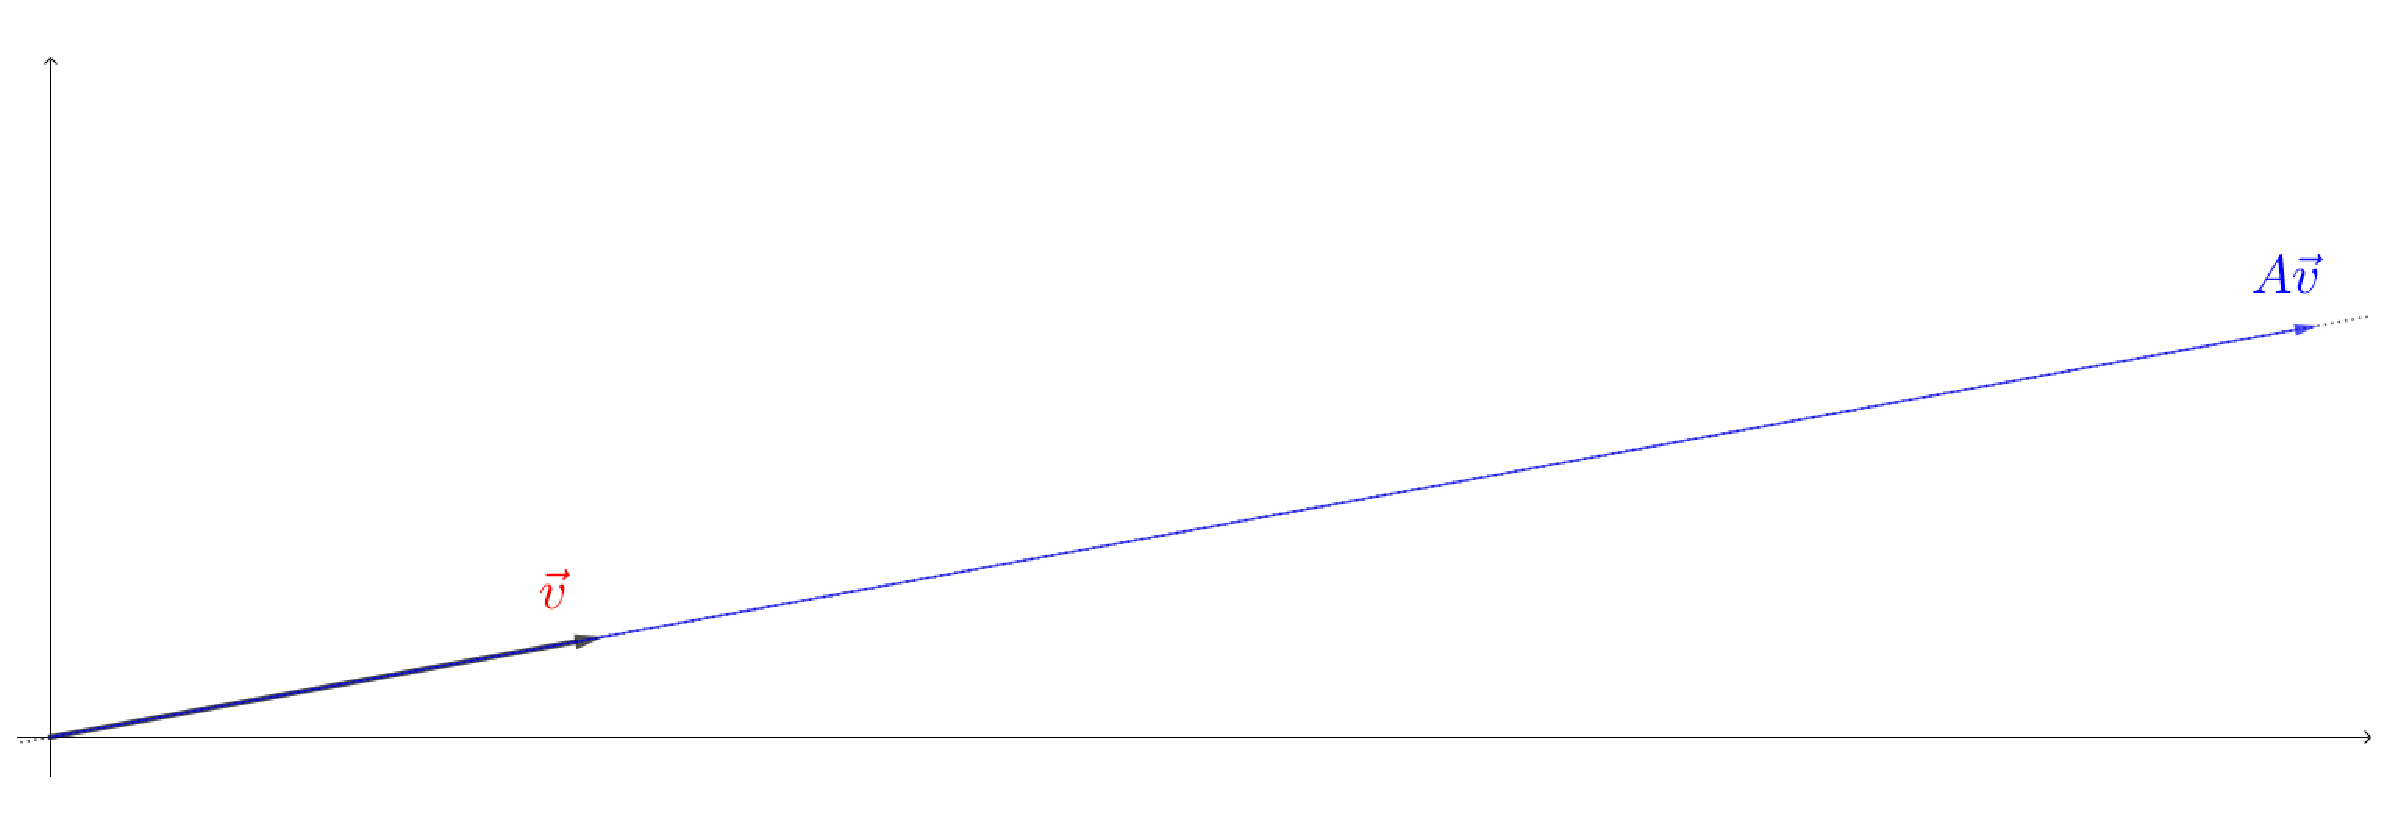
\includegraphics[width=0.3 \linewidth]{\dir/Semana10/semana10-eigen}
	\end{center}
\end{figure}

Ver tamb�m anima��o em \href{https://en.wikipedia.org/wiki/Eigenvalues_and_eigenvectors#Matrix_examples}{wikipedia.org}

\begin{example}
	Considere a matriz
	\[
	A={\begin{bmatrix}2&0&0\\0&3&4\\0&4&9\end{bmatrix}}.
	\] Temos que $\lambda_1 = 2$ � um autovalor desta matriz, porque o vetor
	\[
	\vec{v}_1 =
	{\begin{bmatrix}1\\0\\0\end{bmatrix}} \quad \text{ satisfaz } \quad {\begin{bmatrix}2&0&0\\0&3&4\\0&4&9\end{bmatrix}} {\begin{bmatrix}1\\0\\0\end{bmatrix}} = 2 \cdot {\begin{bmatrix}1\\0\\0\end{bmatrix}}.
	\] Assim, podemos dizer que $\vec{v}_1$ � um autovetor de $A$ associado ao autovalor $2$. Pensando de outra maneira, temos que
	\[
	\vec{v}_2 =
	{\begin{bmatrix}0\\1\\2\end{bmatrix}} \quad \text{ � um autovetor de $A$, pois } \quad {\begin{bmatrix}2&0&0\\0&3&4\\0&4&9\end{bmatrix}} {\begin{bmatrix}0\\1\\2\end{bmatrix}} = {\begin{bmatrix}0\\11\\22\end{bmatrix}} = 11 \cdot {\begin{bmatrix}0\\1\\2\end{bmatrix}}.
	\] Neste caso, concluimos tamb�m que $11$ � um autovalor de $A. \ \lhd$
\end{example}

Observamos que, se $\vec{v}$ for um autovetor de uma matriz $A$ associado a um autovalor $\lambda$, ent�o qualquer m�ltiplo escalar $\alpha \vec{v}$ tamb�m � um autovetor de $A$ associado a $\lambda$. Logo, o conjunto de todos os autovetores associados a um autovalor $\lambda$, uni�o com o vetor nulo, forma um subespa�o vetorial de $\bR^n$, denominado \textbf{autoespa�o} associado ao autovalor $\lambda$:
\[
\text{autoespa�o associado a } \lambda = \big\{ \vec{v} \in \bR^n \, | \, \vec{v} \text{ � autovetor associado a } \lambda \big\} \cup \{\, \vec{0}\, \}.
\]

Vamos analisar uma forma de encontrar os autovalores de uma matriz $A$ de forma sistem�tica. Temos as seguintes equival�ncias:
\begin{align*}
& \lambda \text{ � um autovalor de $A$} \\
\iff & \text{existe } \vec{v} \neq \vec{0} \text{ tal que } A \vec{v} = \lambda \vec{v} \\
\iff & \text{existe } \vec{v} \neq \vec{0} \text{ tal que } (A - \lambda I)\vec{v} = \vec{0} \\
\iff & \text{o sistema homog�neo } (A - \lambda I)\vec{v} = \vec{0} \text{ admite solu��o n�o trivial} \\
\iff & A - \lambda I \text{ n�o � invert�vel} \\
\iff & \det (A - \lambda I) = 0.
\end{align*}
Esta �ltima equa��o pode ser utilizada para encontrar os autovalores: s�o as ra�zes do \textbf{polin�mio caracter�stico}
\[
p(\lambda) = \det (A - \lambda I).
\] A equa��o $\det (A - \lambda I) = 0$ � tamb�m chamada de \textbf{equa��o caracter�stica}. Observe, pelas propriedades dos determinantes, que $p$ � de fato um polin�mio e tem grau $n$, que � igual a ordem da matriz $A$. � assim consequ�ncia do Teorema Fundamental da �lgebra que existem no m�ximo $n$ autovalores reais (j� que um polin�mio de grau $n\ge 1$ possui exatamente $n$ ra�zes complexas).


\begin{example}\label{2x2}
	Vamos encontrar os autovalores de
	\[
	A =
	\left[
	\begin{array}{cc}
	4 & 3 \\
	1 & 2 \\
	\end{array}
	\right].
	\] Precisamos calcular
	\[
	\det\left[
	\begin{array}{cc}
	4-\lambda & 3 \\
	1 & 2-\lambda \\
	\end{array}
	\right] = (4-\lambda)(2-\lambda) - 3 \cdot 1 = \lambda^2 -6\lambda + 5,
	\] que tem ra�zes
	\[
	\lambda = \frac{6 \pm \sqrt{36 - 20}}{2} = 3 \pm 2.
	\] Portanto, $A$ tem dois autovalores reais: $\lambda_1 = 1$ e $\lambda_2 = 5$.
\end{example}


\begin{example}\label{3x3}
	Encontrar os autovalores de
	\[
	A =
	\left[
	\begin{array}{ccc}
	5 & 8 & 16 \\
	4 & 1 & 8 \\
	-4 & -4 & -11 \\
	\end{array}
	\right].
	\] Precisamos calcular
        \begin{align*}
	p(\lambda) = \det (A-\lambda I) & = \det
	\left[
	\begin{array}{ccc}
	5-\lambda & 8 & 16 \\
	4 & 1-\lambda & 8 \\
	-4 & -4 & -11-\lambda \\
	\end{array}
	\right] \\
	& = (5-\lambda) \cdot
	\left|
	\begin{array}{cc}
	1-\lambda & 8 \\
	-4 & -11-\lambda \\
	\end{array}
	\right| -8 \cdot
	\left|
	\begin{array}{cc}
	4 & 8 \\
	-4 & -11-\lambda \\
	\end{array}
	\right| + 16 \cdot
	\left|
	\begin{array}{cc}
	4 & 1-\lambda \\
	-4 & -4 \\
	\end{array}
	\right| \\
	& = (5-\lambda)\big[ (1-\lambda)(-11-\lambda) +32 \big] - 8 \big[ -44-4\lambda +32 \big] + 16 (-16 + 4 -4\lambda) \\
	& = (5-\lambda)\big[ \lambda^2 + 10 \lambda + 21 \big] + 32 \lambda + 12 \cdot 8 - 64\lambda - 12\cdot 16 \\
	& = -\lambda^3 - 5 \lambda^2 + 29 \lambda + 105  - 32 \lambda - 96 \\
	& = -\lambda^3 - 5 \lambda^2 - 3 \lambda + 9.
          \end{align*}
          As poss�veis ra�zes racionais desse polin�mio s� podem ser os divisores do termo independente acima: $\pm 1, \pm 3, \pm9$. Verificamos que $1$ � raiz. Logo, dividindo $p(\lambda)$ por $\lambda - 1$:
	\[
	-\lambda^3 - 5 \lambda^2 - 3 \lambda + 9 = -(\lambda - 1)(\lambda^2 + 6\lambda + 9) = -(\lambda - 1)(\lambda + 3)^2.
	\] Portanto, os autovalores de $A$ s�o $\lambda_1 = 1$ e $\lambda_2 = 3$. Observamos que $3$ � uma raiz de multiplicidade $2$ do polin�mio caracter�stico. $\, \lhd$
\end{example}

O problema deste m�todo de encontrar os autovalores � que nem sempre � f�cil encontrar ra�zes de polin�mios. De fato, encontrar ra�zes de polin�mios pode ser bem complicado mesmo quando o grau do polin�mio � baixo.

Por outro lado, uma vez que os autovalores s�o conhecidos, encontrar os autovetores � um c�lculo direto: basta resolver o sistema linear homog�neo
\[
\big( A - \lambda I \big) \vec{v} = \vec{0}.
\] Isto � outra forma de dizer que o autoespa�o associado a $\lambda$ � o espa�o nulo $\Nul (A - \lambda I)$. Vejamos como far�amos isto nos exemplos anteriores.

\begin{example}[de volta ao Exemplo \ref{2x2}]
	Para encontrar os autovetores de
	\[
	A =
	\left[
	\begin{array}{cc}
	4 & 3 \\
	1 & 2 \\
	\end{array}
	\right]
	\] associados com o autovalor $\lambda_1 = 1$, vamos resolver o sistema homog�neo:
	\[
	\left[
	\begin{array}{cc}
	4-\lambda & 3 \\
	1 & 2-\lambda \\
	\end{array}
	\right] \left[
	\begin{array}{c}
	v_1 \\
	v_2 \\
	\end{array}
	\right] = \left[
	\begin{array}{c}
	0 \\
	0 \\
	\end{array}
	\right] \leftrightsquigarrow
	\left[
	\begin{array}{cc}
	3 & 3 \\
	1 & 1 \\
	\end{array}
	\right] \left[
	\begin{array}{c}
	v_1 \\
	v_2 \\
	\end{array}
	\right] = \left[
	\begin{array}{c}
	0 \\
	0 \\
	\end{array}
	\right].
	\] J� que o sistema � homog�neo, n�o � necess�rio escrever a �ltima coluna de zeros na matriz aumentada associada (no entanto, � necess�rio lembrar que h� uma coluna de zeros). Escalonando
	\[
	\left[
	\begin{array}{cc}
	3 & 3 \\
	1 & 1 \\
	\end{array}
	\right] \sim
	\left[
	\begin{array}{cc}
	1 & 1 \\
	0 & 0 \\
	\end{array}
	\right] \leftrightsquigarrow
	\left\{
	\begin{array}{ll}
	v_1 + v_2 = 0 \\
	\hbox{1 vari�vel livre.}
	\end{array}
	\right.
	\] Em forma vetorial param�trica:
	\[
	\left[
	\begin{array}{c}
	v_1 \\
	v_2 \\
	\end{array}
	\right] =
	\left[
	\begin{array}{c}
	-v_2 \\
	v_2 \\
	\end{array}
	\right] = v_2
	\left[
	\begin{array}{c}
	-1 \\
	1 \\
	\end{array}
	\right] \implies \Nul (A - I) = \Span \left\{ \left[
	\begin{array}{c}
	-1 \\
	1 \\
	\end{array}
	\right] \right\}.
	\]
	
	Para encontrar os autovetores associados a $\lambda_2 = 5$, resolvemos
	\[
	\left[
	\begin{array}{cc}
	4-\lambda & 3 \\
	1 & 2-\lambda \\
	\end{array}
	\right] =
	\left[
	\begin{array}{cc}
	-1 & 3 \\
	1 & -3 \\
	\end{array}
	\right] \sim
	\left[
	\begin{array}{cc}
	1 & -3 \\
	0 &  0 \\
	\end{array}
	\right] \leftrightsquigarrow
	\left\{
	\begin{array}{ll}
	v_1 - 3 v_2 = 0 \\
	\hbox{1 vari�vel livre.}
	\end{array}
	\right.
	\] Em forma vetorial param�trica:
	\[
	\left[
	\begin{array}{c}
	v_1 \\
	v_2 \\
	\end{array}
	\right] =
	\left[
	\begin{array}{c}
	3v_2 \\
	v_2 \\
	\end{array}
	\right] = v_2
	\left[
	\begin{array}{c}
	3 \\
	1 \\
	\end{array}
	\right] \implies \Nul (A - 5 I) = \Span \left\{ \left[
	\begin{array}{c}
	3 \\
	1 \\
	\end{array}
	\right] \right\}.
	\]
\end{example}

\begin{example}[de volta ao Exemplo \ref{3x3}]
	Vamos encontrar os autovetores de
	\[
	A =
	\left[
	\begin{array}{ccc}
	5 & 8 & 16 \\
	4 & 1 & 8 \\
	-4 & -4 & -11 \\
	\end{array}
	\right].
	\]
	
	\begin{itemize}
		\item associados com o autovalor $\lambda_1 = 1$, vamos resolver o sistema homog�neo:
		\[
		\left[
		\begin{array}{ccc}
		5-\lambda_1 & 8 & 16 \\
		4 & 1-\lambda_1 & 8 \\
		-4 & -4 & -11-\lambda_1 \\
		\end{array}
		\right] \left[
		\begin{array}{ccc}
		v_1 \\
		v_2 \\
		v_3 \\
		\end{array}
		\right] = \left[
		\begin{array}{ccc}
		0 \\
		0 \\
		0 \\
		\end{array}
		\right].
		\] Por escalonamento,
		\[
		\left[
		\begin{array}{ccc}
		4 &  8 & 16 \\
		4 &  0 & 8 \\
		-4 & -4 & -12 \\
		\end{array}
		\right] \sim \left[
		\begin{array}{ccc}
		1 &  2 & 4 \\
		0 & -8 & -8 \\
		0 &  4 & 4 \\
		\end{array}
		\right] \sim \left[
		\begin{array}{ccc}
		1 &  2 & 4 \\
		0 &  1 & 1 \\
		0 &  0 & 0 \\
		\end{array}
		\right] \sim \left[
		\begin{array}{ccc}
		1 &  0 & 2 \\
		0 &  1 & 1 \\
		0 &  0 & 0 \\
		\end{array}
		\right] \leftrightsquigarrow
		\left\{
		\begin{array}{ll}
		v_1 + 2 v_3 = 0 \\
		v_2 + v_3 = 0 \\
		v_3  \hbox{ livre}
		\end{array}
		\right.
		\] Em forma param�trica, os autovetores s�o
		\[
		\left[
		\begin{array}{ccc}
		v_1 \\
		v_2 \\
		v_3 \\
		\end{array}
		\right] =
		\left[
		\begin{array}{ccc}
		-2v_3 \\
		-v_3 \\
		v_3 \\
		\end{array}
		\right] = v_3
		\left[
		\begin{array}{ccc}
		-2 \\
		-1 \\
		1 \\
		\end{array}
		\right]  \implies \Nul (A - I) = \Span \left\{ \left[
		\begin{array}{c}
		-2 \\
		-1 \\
		1 \\
		\end{array}
		\right] \right\}.
		\]
		\item associados com o autovalor $\lambda_2 = -3$, vamos resolver o sistema homog�neo:
		\[
		\left[
		\begin{array}{ccc}
		5-\lambda_2 & 8 & 16 \\
		4 & 1-\lambda_2 & 8 \\
		-4 & -4 & -11-\lambda_2 \\
		\end{array}
		\right] \left[
		\begin{array}{ccc}
		v_1 \\
		v_2 \\
		v_3 \\
		\end{array}
		\right] = \left[
		\begin{array}{ccc}
		0 \\
		0 \\
		0 \\
		\end{array}
		\right].
		\] Por escalonamento,
		\[
		\left[
		\begin{array}{ccc}
		8 &  8 & 16 \\
		4 &  4 & 8 \\
		-4 & -4 & -8 \\
		\end{array}
		\right] \sim \left[
		\begin{array}{ccc}
		1 &  1 & 2 \\
		0 &  0 & 0 \\
		0 &  0 & 0 \\
		\end{array}
		\right] \leftrightsquigarrow
		\left\{
		\begin{array}{ll}
		v_1 + v_2 + 2v_3 = 0 \\
		\hbox{2 vari�veis livres}
		\end{array}
		\right.
		\] Em forma param�trica, os autovetores s�o
		\[
		\left[
		\begin{array}{ccc}
		v_1 \\
		v_2 \\
		v_3 \\
		\end{array}
		\right] =
		\left[
		\begin{array}{ccc}
		- v_2 - 2 v_3 \\
		v_2 \\
		v_3 \\
		\end{array}
		\right] = v_2
		\left[
		\begin{array}{ccc}
		-1 \\
		1 \\
		0 \\
		\end{array}
		\right] + v_3
		\left[
		\begin{array}{ccc}
		-2 \\
		0 \\
		1 \\
		\end{array}
		\right] \implies \Nul (A - I) = \Span \left\{ \left[
		\begin{array}{c}
		-1 \\
		1 \\
		0 \\
		\end{array}
		\right], \left[
		\begin{array}{ccc}
		-2 \\
		0 \\
		1 \\
		\end{array}
		\right] \right\}. \lhd
		\]
	\end{itemize}
\end{example}

Observamos que, nos exemplos anteriores, a dimens�o do autoespa�o associado ficou igual � multiplicidade do autovalor. \textbf{Isto nem sempre � verdade}. Como exerc�cio, verifique que a dimens�o do autoespa�o associado ao autovalor $\lambda = 1$ da matriz
\[
\begin{bmatrix}
1 & 1 \\ 0 & 1
\end{bmatrix}
\] � igual a $1$, embora a multiplicidade do autovalor seja $2$.

De forma geral, chamamos a multiplicidade do autovalor de \textbf{multiplicidade alg�brica}, enquanto que a dimens�o do autoespa�o associado � chamada de \textbf{multiplicidade geom�trica}.


\section{Diagonaliza��o}

Matrizes diagonais s�o matrizes da forma
\[
\begin{bmatrix}
\lambda_1 & 0 & 0 & \cdots & 0 \\
0 & \lambda_2 & 0 & \cdots & 0 \\
0 & 0 & \lambda_3 & \cdots & 0 \\
\vdots & \vdots & \vdots & \ddots & \vdots \\
0 & 0 & 0 & \cdots & \lambda_n \\
\end{bmatrix}.
\] J� que s�o triangulares, seus autovalores s�o os elementos da diagonal principal. Observamos tamb�m que os autovetores associados s�o os elementos da base can�nica de $\bR^n$.

Na realidade, sempre que � poss�vel formar uma base do espa�o $\bR^n$ apenas com autovetores, � poss�vel fazer uma mudan�a de bases de modo que a representa��o da matriz � diagonal, com os autovalores na diagonal principal. De fato, montando uma matriz $P$ com os autovetores
\[
P = \begin{bmatrix}
| & | &  & | \\
\vec{v}_1 & \vec{v}_2 & \cdots & \vec{v}_n \\
| & | &  & |\\
\end{bmatrix} \implies P^{-1} A P = D = \begin{bmatrix}
\lambda_1 & 0  & \cdots & 0 \\
0 & \lambda_2  & \cdots & 0 \\
\vdots & \vdots & \ddots & \vdots \\
0 & 0 & \cdots & \lambda_n \\
\end{bmatrix}.
\]

\begin{example}[de volta ao Exemplo \ref{3x3}]
	Vimos que, para a matriz
	\[
	A =
	\left[
	\begin{array}{ccc}
	5 & 8 & 16 \\
	4 & 1 & 8 \\
	-4 & -4 & -11 \\
	\end{array}
	\right],
	\] temos autovalores $\lambda_1 = 1$ e $\lambda_2 = -3$ e autoespa�os associados:
	\[
	\Nul (A - I) = \Span \left\{ \left[
	\begin{array}{c}
	-2 \\
	-1 \\
	1 \\
	\end{array}
	\right] \right\}; \qquad \Nul (A - I) = \Span \left\{ \left[
	\begin{array}{c}
	-1 \\
	1 \\
	0 \\
	\end{array}
	\right], \left[
	\begin{array}{ccc}
	-2 \\
	0 \\
	1 \\
	\end{array}
	\right] \right\}.
	\] Montamos a matriz
	\[
	P =
	\begin{bmatrix}
	-2&-1&-2 \\ -1&1&0 \\ 1&0&1
	\end{bmatrix}
	\] Por escalonamento, podemos calcular a matriz inversa
	\[
	P^{-1} =
	\begin{bmatrix}
	-1&-1&-2 \\ -1&0&-2 \\ 1&1&3
	\end{bmatrix}
	\] e temos
          \begin{align*}
	P^{-1} A P & =
	\begin{bmatrix}
	-1&-1&-2 \\ -1&0&-2 \\ 1&1&3
	\end{bmatrix}
	\begin{bmatrix}
	5 & 8 & 16 \\ 4 & 1 & 8 \\ -4 & -4 & -11 \\
	\end{bmatrix}
	\begin{bmatrix}
	-2&-1&-2 \\ -1&1&0 \\ 1&0&1
	\end{bmatrix} \\
	& =
	\begin{bmatrix}
	-1&-1&-2 \\ 3&0&6 \\ -3&-3&-9
	\end{bmatrix}
	\begin{bmatrix}
	-2&-1&-2 \\ -1&1&0 \\ 1&0&1
	\end{bmatrix} =
	\begin{bmatrix}
	1&0&0 \\ 0&-3&0 \\ 0&0&-3
	\end{bmatrix}. \ \lhd
          \end{align*}
\end{example}

Nem todas as matrizes s�o diagonaliz�veis, como acima. J� vimos que isto � poss�vel quando uma base de autovetores existe. No exemplo
\[
A = \begin{bmatrix}
2&1 \\ 0&2
\end{bmatrix}
\] n�o h� dois autovetores linearmente independentes e, portanto, n�o � poss�vel diagonalizar a matriz $A$.


\vspace{0.3cm}

Em geral, valem as seguintes propriedades: seja $A$ uma matriz de orden $n \times n$. Ent�o:
\begin{itemize}
	\item Se $A$ possui $n$ autovalores reais distintos, ent�o $A$ possui uma base de autovetores e � diagonaliz�vel, pois possui um autovetor associado a cada um dos seus autovalores distintos.
	\item No caso de $A$ possuir autovalores reais com multiplicidade maior do que $1$, $A$ apenas ser� diagonaliz�vel se cada autovalor de multiplicidade $k$ tiver $k$ autovetores linearmente independentes. Em outras palavras, s� ser� poss�vel formar uma base de autovetores de $A$ quando 
	\[
	\Dim \Nul (A - \lambda I) = \text{ multiplicidade do autovalor } \lambda.
	\]
	\item Caso $\dim \Nul (A - \lambda I)$ seja menor do que a multiplicidade do autovalor $\lambda$ ou $A$ possua autovalores complexos, ent�o $A$ n�o � diagonaliz�vel.
\end{itemize}


\begin{example}
	A matriz
	\[
	A = \begin{bmatrix}
	2&1 \\ -1&2
	\end{bmatrix}
	\] tem polin�mio caracter�stico 
	\[
	p(\lambda) = \det \begin{bmatrix}
	2-\lambda&1 \\ -1&2-\lambda
	\end{bmatrix} = (2-\lambda)^2 +1 = \lambda^2 -4\lambda +5
	\] cujas ra�zes s�o $\lambda = \frac{4 \pm 3i}{2}$. Logo, $A$ n�o � diagonaliz�vel.
\end{example}


\end{document} 
 %Este trabalho está licenciado sob a Licença Creative Commons Atribuição-CompartilhaIgual 3.0 Não Adaptada. Para ver uma cópia desta licença, visite http://creativecommons.org/licenses/by-sa/3.0/ ou envie uma carta para Creative Commons, PO Box 1866, Mountain View, CA 94042, USA.

\documentclass[../livro.tex]{subfiles}  %%DM%%Escolher document class and options article, etc

%define o diretório principal
\providecommand{\dir}{..}

%%%%%%%%%%%%%%%%%%%%%%%%%%%%%%%%%%%%%%%%%%%%%
%%%%%%%%%%%%INICIO DO DOCUMENTO%%%%%%%%%%%%%%
%%%%%%%%%%%%%%%%%%%%%%%%%%%%%%%%%%%%%%%%%%%%%

\begin{document}

\chapter{Semana 11}


Nesta semana, nós começamos uma abordagem um pouco mais geométrica de espaços vetoriais: ângulo entre vetores, comprimento de vetores, ortogonalidade. Estes conceitos já são de nossa familiaridade da geometria euclideana (em $\mathbb{R}^2$ e $\mathbb{R}^3$). No entanto, é também nosso objetivo estender estes conceitos para dimensões maiores do que $3$.


\section{Comprimento, ângulos e o produto escalar}

Se, na base canônica (isto é, no sistema de coordenadas usual) do espaço $\mathbb{R}^3$, representamos um vetor por
\begin{equation}
\vec{v} =
\begin{bmatrix}
v_1 \\ v_2 \\ v_3
\end{bmatrix},
\end{equation} então o seu \textbf{comprimento} (ou \textbf{magnitude} ou \textbf{norma}) é dado por
\begin{equation}
\|\vec{v}\| = \sqrt{v_1^2 + v_2^2 + v_3^2}.
\end{equation} Esta é uma instância do Teorema de Pitágoras\footnote{Duas aplicações do Teorema de Pitágoras usual do plano. Uma para obter o comprimento $\sqrt{v_1^2 + v_2^2}$ da diagonal que está no plano $xy$ e a outra para obter $\|\vec{v}\|$.}.

\begin{figure}[h!]
	\begin{center}
		\includegraphics[width=0.3\linewidth]{\dir/Semana11/semana11-coord}
	\end{center}
\end{figure}

\noindent A definição acima pode ser generalizada para dimensão $n$ qualquer:
\begin{equation}
\vec{v} =
\begin{bmatrix}
v_1 \\ v_2 \\ \vdots \\ v_n
\end{bmatrix} \quad \rightsquigarrow \quad \|\vec{v}\| = \sqrt{v_1^2 + v_2^2 + \cdots + v_n^2}.
\end{equation}


O \textbf{produto escalar} ou \textbf{produto interno} entre dois vetores $\vec{v}$ e $\vec{w}$ é um número (também dito escalar) associado com estes dois vetores. Em coordenadas, se $\vec{v} = (v_1, v_2, v_3)$ e $\vec{w} = (w_1, w_2, w_3)$ são vetores do espaço tridimensional $\mathbb{R}^3$, temos
\begin{equation}
\vec{v} \cdot \vec{w} = v_1 w_1 + v_2 w_2 + v_3 w_3.
\end{equation} Vejamos que realmente o produto escalar tem a ver com o ângulo entre dois vetores. Isto é uma consequência da Lei dos Cossenos, que nos diz que
\begin{equation}
\|\vec{v} - \vec{w}\|^2 = \|\vec{v}\|^2 + \|\vec{w}\|^2 - 2 \|\vec{v}\| \|\vec{w}\| \cos \theta,
\end{equation} onde $\theta$ é o ângulo entre $\vec{v}$ e $\vec{w}$. 

	\begin{center}
		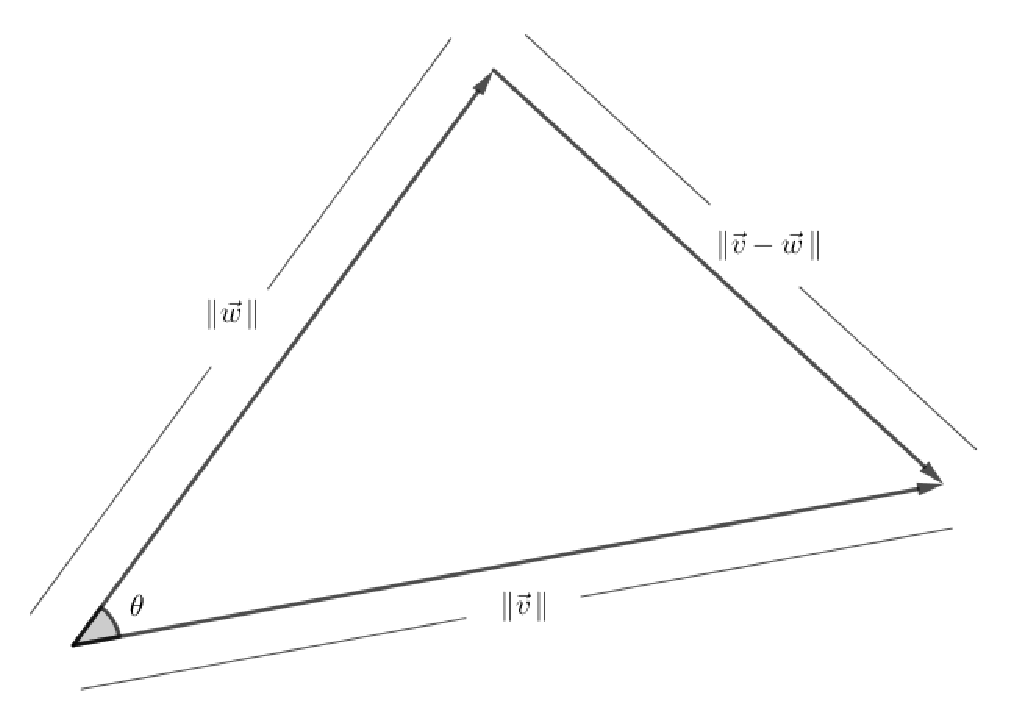
\includegraphics[width=0.7\linewidth]{\dir/Semana11/semana11-cossenos}
	\end{center}

\noindent Escrevendo estes comprimentos em termos das coordenadas e fazendo os cancelamentos necessários, chegamos na seguinte identidade:
\begin{equation}
v_1 w_1 + v_2 w_2 + v_3 w_3 = \|\vec{v}\| \|\vec{w}\| \cos \theta, \quad \text{ isto é,} \quad \vec{v} \cdot \vec{w} = \|\vec{v}\| \|\vec{w}\| \cos \theta.
\end{equation}


Motivados pelos conceitos acima, consideramos
\begin{equation}
\vec{x} =
\begin{bmatrix}
x_1 \\ x_2 \\ \vdots \\ x_n
\end{bmatrix} \quad \text{e} \quad \vec{y} =
\begin{bmatrix}
y_1 \\ y_2 \\ \vdots \\ y_n
\end{bmatrix}
\end{equation} vetores de $\mathbb{R}^n$ representados na base canônica, e definimos o \textbf{produto escalar} ou \textbf{produto interno} entre $\vec{x}$ e $\vec{y}$:
\begin{equation}
\vec{x} \cdot \vec{y} = x_1 y_1 + x_2 y_2 + \cdots + x_n y_n.
\end{equation} O ângulo entre $\vec{x}$ e $\vec{y}$, para $n$ qualquer, pode então ser \textit{definido} pela equação
\begin{equation}
\cos \theta = \frac{\vec{x} \cdot \vec{y}}{\|\vec{x}\| \|\vec{y}\|}.
\end{equation} Embora abstratos, estes conceitos são bem fundamentados geometricamente. Dois vetores (linearmente independentes) de um espaço vetorial $n$-dimensional geram um subespaço vetorial de dimensão $2$. Este pode, por sua vez, pode ser pensado como um plano que passa pela origem de $\mathbb{R}^n$. Assim, podemos imaginar o ângulo entre estes vetores naturalmente.

\begin{proposition}[Principais propriedades do produto escalar]
	Para $\vec{x}, \vec{y}, \vec{z} \in \mathbb{R}^n$ e $c \in \mathbb{R}$ um escalar, temos as seguintes propriedades
	\begin{enumerate}
		\item  $\vec{x} \cdot \vec{y} = \vec{y} \cdot \vec{x}$
		\item  $(\vec{x} + \vec{y}) \cdot \vec{z} = \vec{x} \cdot \vec{z} + \vec{y} \cdot \vec{z}$
		\item  $(c\vec{x}) \cdot \vec{y} = c \vec{x} \cdot \vec{y} = \vec{x} \cdot (c\vec{y})$
		\item  $\vec{x} \cdot \vec{x} \ge 0$ e $\, \vec{x} \cdot \vec{x} = 0$ se, e somente se, $\vec{x} = \vec{0}$;
		\item  $\|\vec{x}\| = \sqrt{\vec{x} \cdot \vec{x}}$;
		\item  $\| c \vec{x} \| =  |c| \| \vec{x} \|$.
	\end{enumerate}
\end{proposition}

Estas propriedades são todas de fácil verificação (e são deixadas para o leitor verificar, como exercício).

\begin{example}
	Considere os vetores de $\mathbb{R}^5$ escritos na base canônica:
	\begin{equation}
	\vec{x} =
	\begin{bmatrix}
	-1 \\ 2 \\ 0 \\ 3 \\ -1
	\end{bmatrix} \quad \text{e} \quad \vec{y} =
	\begin{bmatrix}
	4 \\ 3 \\ -1 \\ -11 \\ 1
	\end{bmatrix}
	\end{equation} Assim, temos
	\begin{equation}
	\vec{x} \cdot \vec{y} = (-1)\cdot 4 + 2 \cdot 3 + 0 \cdot (-1) +3 \cdot(-11) + (-1)\cdot 1 = -4 + 6 +0 -33 -1 = -31.
	\end{equation} Da mesma forma, podemos calcular os comprimentos
	\begin{equation}
	\| \vec{x} \| = \sqrt{(-1)^2 + 2^2 + 0^2 + 3^2 + (-1)^2} = \sqrt{15} \quad \text{e} \quad \| \vec{y} \| = \sqrt{4^2 + 3^2 + (-1)^2 + (-11)^2 + 1^2} = \sqrt{148}.
	\end{equation} Logo, o ângulo $\theta$ entre estes vetores satisfaz (utilizamos uma calculadora para calcular as raízes quadradas e a função inversa do cosseno):
	\begin{equation}
	\cos \theta = \frac{\vec{x} \cdot \vec{y}}{\|\vec{x}\| \|\vec{y}\|} = \frac{-31}{\sqrt{15} \, \sqrt{148}} \simeq -0,65794 \implies  \theta \simeq 2,28887634 \textrm{ radianos} \simeq 131,12^{\text{o}}. \ \lhd
	\end{equation}
\end{example}

\begin{example}
	Considere um vetor tridimensional
	\begin{equation}
	\vec{u} =
	\begin{bmatrix}
	2 \\ 3 \\ -1
	\end{bmatrix}.
	\end{equation} Já sabemos a multiplicação de um escalar pelo vetor $\vec{u}$ muda o comprimeto (e talvez também o sentido) do vetor. Por exemplo, se multiplicarmos por $2$, o comprimento será multiplicado por $2$; se dividirmos por $3$, o comprimento será dividido por $3$. Se nós dividirmos pelo próprio comprimento de $\vec{u}$ nós obtemos um vetor unitário. Para verificar analíticamente, basta utilizar a Propriedade \textit{6} acima:
	\begin{equation}
	c = \frac{1}{\|\vec{u}\|} \implies \left\| \frac{\vec{u}}{\|\vec{u}\|} \right\| = \|c \vec{u} \| = c \|\vec{u}\| = \frac{1}{\|\vec{u}\|}\|\vec{u}\| = 1.
	\end{equation} Então se quisermos encontrar um vetor unitário na direção de $\vec{u}$ acima, calculamos
	\begin{equation}
	\|\vec{u}\| = \sqrt{4 + 9 + 1} = \sqrt{14} \quad \rightsquigarrow \quad \vec{v} = \frac{\vec{u}}{\|\vec{u}\|} = \frac{\vec{u}}{\sqrt{14}} =
	\begin{bmatrix}
	2/\sqrt{14} \\ 3/\sqrt{14} \\ -1/\sqrt{14}
	\end{bmatrix}
	\end{equation} é o vetor procurado. Este processo de obter um vetor unitário na mesma direção de um vetor previamente fixado é chamado de \textbf{normalização}. Observe que existem apenas dois vetores unitários na mesma direção de $\vec{u}$, a saber, $\vec{v}$ e $- \vec{v}. \ \lhd$
\end{example}

\subsection*{Exercícios resolvidos}

\construirExeresol

\subsection*{Exercícios}

\construirExer

\section{Ortogonalidade}

Como vimos na seção anterior, o produto escalar está relacionado com o ângulo entre dois vetores pela fórmula
\begin{equation}
\cos \theta = \frac{\vec{x} \cdot \vec{y}}{\|\vec{x}\| \|\vec{y}\|}.
\end{equation} Quando este ângulo $\theta$ é igual a $\pi /2$ (que é equivalente a $90^o$), vale que $\cos \theta = 0$ e logo $\vec{x} \cdot \vec{y} = 0$.

Nós vamos dizer que os dois vetores $\vec{x}$ e $\vec{y}$ são \textbf{ortogonais} quando satisfazem
\begin{equation}
\vec{x} \cdot \vec{y} = 0.
\end{equation} Poderíamos também usar a palavra perpendiculares, mas por algum motivo esta terminologia é bastante menos comum quando lidamos com vetores em espaços vetoriais de dimensão maior do que $3$.

Dizemos também que um conjunto de vetores é um \textbf{conjunto ortogonal} se todo par de vetores do conjunto for ortogonal. Em outras palavras, um conjunto $\{\vec{v}_1, \vec{v}_2, \dots, \vec{v}_k\}$ é um conjunto ortonogonal se, para qualquer escolha de índices $i \neq j$, tivermos $\vec{v}_i \cdot \vec{v}_j = 0$.

Se, além de o conjunto ser ortogonal, todos os seus elementos serem unitários (estarem normalizados), então nós dizemos que o conjunto é um \textbf{conjunto ortonormal}. De outra maneira, um conjunto $\{\vec{v}_1, \vec{v}_2, \dots, \vec{v}_k\}$ é um conjunto ortonormal se, para qualquer índice $i$, $\|\vec{v}_i\| = 1$ e, para qualquer escolha de índices $i \neq j$, tivermos $\vec{v}_i \cdot \vec{v}_j = 0$.\footnote{Uma notação bastante comum, principalmente em matemática e física, é a do delta de Kronecker:\begin{equation} \delta_{ij} = \left\lbrace \begin{array}{l}
	1, \text{ se } i = j \\
	0, \text{ se } i \neq j
	\end{array} \right. . \end{equation} Em notação matricial, $I_k = (\delta_{ij})$ é a matriz identidade. Nesta notação, podemos dizer, mais sucintamente, que um conjunto $\{\vec{v}_1, \vec{v}_2, \dots, \vec{v}_k\}$ é ortonormal se $\vec{v}_i \cdot \vec{v}_j = \delta_{ij}$ para quaisquer $i,j = 1, 2, 3, \dots, k$.}

\begin{example}
	Os vetores
	\begin{equation}
	\vec{x} = \begin{bmatrix}
	-1 \\ 2
	\end{bmatrix} \quad \text{e} \quad
	\vec{y} = \begin{bmatrix}
	2 \\ 1
	\end{bmatrix}
	\end{equation} são ortogonais, pois $\vec{x} \cdot \vec{y} = (-1)\cdot 2 + 2 \cdot 1 = 0$, enquanto que os vetores
	\begin{equation}
	\vec{w} = \begin{bmatrix}
	1 \\ 2
	\end{bmatrix} \quad \text{e} \quad
	\vec{z} = \begin{bmatrix}
	2 \\ 1
	\end{bmatrix}
	\end{equation} não são ortogonais, já que $\vec{w} \cdot \vec{z} = 1\cdot 2 + 2 \cdot 1 = 4$. Nestes casos, podemso dizer que o conjunto $\{\vec{x}, \vec{y}\}$ é um conjunto ortogonal enquanto $\{\vec{w}, \vec{z}\}$ não é.
\end{example}



\begin{example}
	A base canônica do espaço $\mathbb{R}^n$:
	\begin{equation}
	\vec{e}_1 =
	\begin{bmatrix}
	1 \\ 0 \\ 0 \\ \vdots \\ 0
	\end{bmatrix}, \
	\vec{e}_2 =
	\begin{bmatrix}
	0 \\ 1 \\ 0 \\ \vdots \\ 0
	\end{bmatrix}, \
	\vec{e}_3 =
	\begin{bmatrix}
	0 \\ 0 \\ 1 \\ \vdots \\ 0
	\end{bmatrix}, \ \cdots,
	\vec{e}_n =
	\begin{bmatrix}
	0 \\ 0 \\ 0 \\ \vdots \\ 1
	\end{bmatrix}
	\end{equation} é um conjunto ortogonal, porque quando escolhermos $i\neq j$, temos
	\begin{equation}
	\vec{e}_i \cdot \vec{e}_j = 1 \cdot 0 + 0 \cdot 1 = 0. 
	\end{equation} É também ortonormal, já que, para todo $i$,
	\begin{equation}
	\| \vec{e}_i\|  = \sqrt{0^2 + 0^2 + \cdots + 1^2 + \cdots + 0^2 + 0^2} = 1. \ \lhd
	\end{equation}
\end{example}

Uma primeira propriedade de ortogonalidade é uma versão para espaços vetoriais quaisquer do Teorema de Pitágoras, que aparece naturamente ao considerarmos vetores ortogonais.

\begin{theorem}[Teorema de Pitágoras]
	Se dois vetores $\vec{x}$ e $\vec{y}$ são ortogonais, então
	\begin{equation}
	\|\vec{x} + \vec{y}\|^2 = \|\vec{x}\|^2 + \|\vec{y}\|^2.
	\end{equation}
\end{theorem}

\begin{proof}
	Esperamos que esta demonstração auxilie no compreendimento analítico e geométrico dos conceitos que introduzimos até agora. O vetor $\vec{x} + \vec{y} \,$ pode ser considerado a hipotenusa do triângulo retângulo de catetos $\vec{x}$ e $\vec{y}$ (fazer uma figura!).
	
	Pelas propriedades do comprimento e do produto escalar, temos que, para \textit{quaisquer} dois vetores $\vec{x}$ e $\vec{y}$ (não necessariamente ortogonais), vale que
	\begin{equation}
	\|\vec{x} + \vec{y}\|^2 = (\vec{x} + \vec{y}) \cdot (\vec{x} + \vec{y}) =  \vec{x} \cdot \vec{x} + \vec{x} \cdot \vec{y} +  \vec{y} \cdot \vec{x} +  \vec{y} \cdot \vec{y} = \|\vec{x}\|^2 + 2 (\vec{x} \cdot \vec{y}) + \|\vec{y}\|^2.
	\end{equation} De certa maneira, esta é uma forma de reescrever a Lei dos Cossenos. Quando os vetores $\vec{x}$ e $\vec{y}$ forem ortogonais, temos $\vec{x} \cdot \vec{y} = 0$, concluimos que
	\begin{equation}
	\|\vec{x} + \vec{y}\|^2 = \|\vec{x}\|^2 + \|\vec{y}\|^2. \qedhere
	\end{equation}
\end{proof}


Notamos que, de acordo com a nossa definição, o vetor nulo é ortogonal a qualquer outro. Vejamos, no entanto, que vetores não nulos satisfazem propriedades adicionais.

\begin{theorem}
	Todo conjunto ortogonal $\{\vec{v}_1, \vec{v}_2, \dots, \vec{v}_k\}$ formado por vetores \textit{não nulos} é um conjunto linearmente independente (LI).
\end{theorem}

\begin{proof}
	Considerando uma combinação linear
	\begin{equation}
	c_1 \vec{v}_1 + c_2 \vec{v}_2 + \dots + c_k \vec{v}_k = \vec{0}
	\end{equation} e fazendo o produto escalar com qualquer dos vetores $\vec{v}_j$ na equação acima, concluimos que
	\begin{equation}
	(c_1 \vec{v}_1 + c_2 \vec{v}_2 + \dots + c_k \vec{v}_k ) \cdot \vec{v}_j = \vec{0} \cdot \vec{v}_j.
	\end{equation} Agora, a condição de ortogonalidade nos diz que $\vec{v}_i \cdot \vec{v}_j = 0$ sempre que $i \neq j$. Portanto,
	\begin{equation}
	c_j \| \vec{v}_j \| = c_j (\vec{v}_j \cdot \vec{v}_j) = 0 \stackrel{\vec{v}_j \neq \vec{0}}{\implies} c_j = 0.
	\end{equation} Isto é a definição de um conjunto ser LI: qualquer combinação linear que resulte no vetor nulo deve ter todos os coeficientes nulos.
\end{proof}

\begin{example}
O conjunto 
\begin{equation}
\left\lbrace 
\vec{u}_1 = \begin{bmatrix}
1 \\ 2 \\ 2
\end{bmatrix}, \ 
\vec{u}_2 = \begin{bmatrix}
2 \\ 1 \\ -2
\end{bmatrix}, \ 
\vec{u}_3 = \begin{bmatrix}
2 \\ -2 \\ 1
\end{bmatrix}
\right\rbrace 
\end{equation} pois

\begin{equation}
\begin{split}
\vec{u}_1 \cdot \vec{u}_2 = 2 + 2 - 4 = 0, \\
\vec{u}_1 \cdot \vec{u}_3 = 2 - 4 + 2 = 0, \\
\vec{u}_2 \cdot \vec{u}_3 = 4 - 2 - 2 = 0. 
\end{split} 
\end{equation}
Logo, pelo teorema acima, o conjunto $\{\vec{u}_1, \vec{u}_2,\vec{u}_3\}$ é linearmente independente. Neste exemplo, são todos elementos de $\mathbb{R}^3$; portanto, formam uma base para $\mathbb{R}^3$ que é também ortogonal (voltaremos a falar sobre bases ortogonais em breve)$. \ \lhd$
\end{example}

Uma das aplicações mais importantes do produto escalar reside no fato de nós conseguirmos fazer projeções ortogonais em direções fixadas. Por exemplo, suponhamos que em um sistema físico, um vetor $\vec{v}$ representa a força aplicada em um ponto, como na figura abaixo.
\begin{figure}[h!]
	\begin{center}
		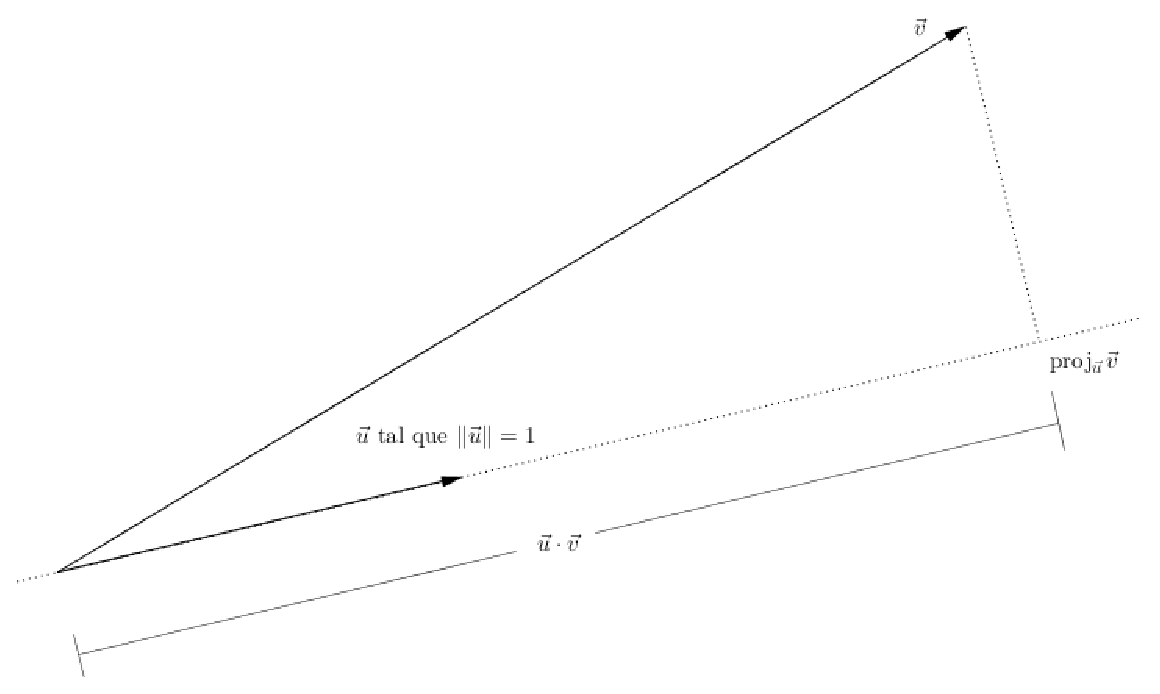
\includegraphics[width=1\linewidth]{\dir/Semana11/semana11-proj}
	\end{center}
\end{figure} Gostaríamos de encontrar a componente do vetor na direção da reta tracejada. Para isto, podemos considerar um vetor \textit{unitário} $\vec{u}$ sobre a reta. Assim, a componente de $\vec{v}$ na direção de $\vec{u}$ é igual a $k \vec{u}$, onde $k$ tem a ver com o cosseno do ângulo entre os vetores:
\begin{equation}
\cos \theta = \frac{\text{cateto adjacente}}{\text{hipotenusa}} = \frac{k}{\|\vec{v}\|}.
\end{equation} Utilizando novamente que $\vec{u}$ é um vetor unitário (isto é, $\|\vec{u}\|=1$), concluimos que
\begin{equation}
k = \|\vec{v}\| \cos \theta = \|\vec{u}\| \|\vec{v}\| \cos \theta = \vec{u} \cdot \vec{v}.
\end{equation} Assim sendo, definimos a \textbf{projeção ortogonal de $\vec{v}$ em um vetor unitário $\vec{u}$} como sendo
\begin{equation}
\boxed{\proj_{\vec{u}} \vec{v} = (\vec{u} \cdot \vec{v}) \, \vec{u}.}
\end{equation} No \textbf{caso onde $\vec{u}$ não está normalizado}, devemos primeiramente normalizar o vetor, de modo que a projeção ortogonal é dada por
\begin{equation}
\boxed{\proj_{\vec{u}} \vec{v} = \bigg( \frac{\vec{u}}{\|\vec{u}\|} \cdot \vec{v} \bigg) \, \frac{\vec{u}}{\|\vec{u}\|} = \frac{\vec{u} \cdot \vec{v}}{\|\vec{u}\|^2} \, \vec{u} = \frac{\vec{u} \cdot \vec{v}}{\vec{u} \cdot \vec{u}} \, \vec{u}.}
\end{equation}

\begin{example}\label{canon}
	Considere vetores no espaço de quatro dimensões $\mathbb{R}^4$. Vamos determinar a projeção do vetor $\vec{v} =
	\begin{bmatrix}
	1 \\ -1 \\ 3 \\ 4
	\end{bmatrix}$ na direção da reta que tem a mesma direção do vetor $\vec{u} =
	\begin{bmatrix}
	1 \\ 1 \\ 1 \\ -1
	\end{bmatrix}.$ Observamos inicialmente que $\|\vec{u}\| = \sqrt{4} = 2$ não é unitário. Temos que
	\begin{equation}
	\proj_{\vec{u}} \vec{v} =  \frac{\vec{u} \cdot \vec{v}}{\|\vec{u}\|^2} \, \vec{u} = \frac{1 - 1 + 3 - 4}{4}
	\begin{bmatrix}
	1 \\ 1 \\ 1 \\ -1
	\end{bmatrix} =
	-\frac{1}{4}
	\begin{bmatrix}
	1 \\ 1 \\ 1 \\ -1
	\end{bmatrix} =
	\begin{bmatrix}
	1/4 \\ 1/4 \\ 1/4 \\ -1/4
	\end{bmatrix}.
	\end{equation} A projeção de $\vec{v}$ sobre o vetor $\vec{e}_3$ da base canônica de $\mathbb{R}^4$ é (observe que $\|\vec{e}_3\| = 1$)
	\begin{equation}
	\proj_{\vec{e}_3} \vec{v} = (\vec{e}_3 \cdot \vec{v}) \, \vec{e}_3 = (0 + 0 + 3 + 0)
	\begin{bmatrix}
	0 \\ 0 \\ 1 \\ 0
	\end{bmatrix} = \begin{bmatrix}
	0 \\ 0 \\ 3 \\ 0
	\end{bmatrix}.
	\end{equation} Observe que a projeção sobre o vetor $\vec{e}_3$ da base canônica apenas ``enfatiza'' a terceira componente do vetor $\vec{v}$. Isto é bastante natural, pois $\vec{v} \cdot \vec{e}_3$ deve fornecer o comprimento da projeção de $\vec{v}$ na direção do vetor unitário $\vec{e}_3$, que deve ser igual a terceira componente do vetor. É justamente assim que usamos a base canônica para representar vetores geometricamente. De forma geral, podemos escrever
	\begin{equation}
	\vec{v} = \big( \vec{v} \cdot \vec{e}_1 \big) \vec{e}_1 + \big( \vec{v} \cdot \vec{e}_2 \big) \vec{e}_2  + \big( \vec{v} \cdot \vec{e}_3 \big) \vec{e}_3  + \big( \vec{v} \cdot \vec{e}_4 \big) \vec{e}_4.
	\end{equation} Este tipo de represetação será explorado com mais detalhes na próxima seção$. \ \lhd$
\end{example}

As projeções ortogonais também podem ser utilizadas para o cálculo de distâncias de ponto à retas que passam pela origem: Pela interpretação geométrica da subtração de vetores, obtemos um vetor perpendicular à reta com a direção de $\vec{u}$ e que termina onde termina o vetor $\vec{v}$ (ver figura).
\begin{figure}[h!]
	\begin{center}
		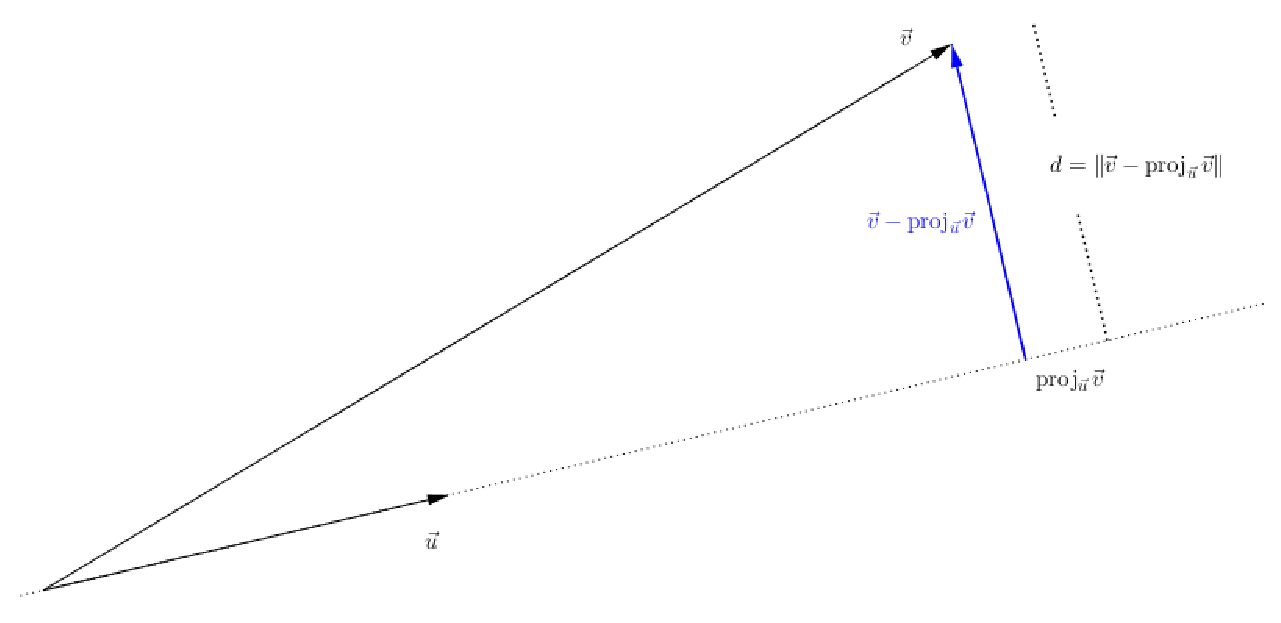
\includegraphics[width=1\linewidth]{\dir/Semana11/semana11-dist}
	\end{center}
\end{figure}

\noindent Desta maneira, o comprimento deste vetor, a saber $\|\vec{u} - \proj_{\vec{u}} \vec{v}\|$, é a distância procurada.\footnote{Lembre: a distância de um ponto a uma reta é a menor distância entre este ponto e os pontos da reta; por esta razão que procuramos um vetor perpendicular à reta.}

\begin{example}
	Calcular a distância do ponto $P = (0,2,3)$ e a reta que passa pela origem e tem a direção do vetor $\vec{u} =
	\begin{bmatrix}
	1 \\ 2 \\1
	\end{bmatrix}.$
	
	Para isto, consideramos o vetor $\vec{v}$ cujas componentes são as componentes do ponto $P$. Assim, estamos na situação da discussão acima e vale que
	\begin{equation}
	\proj_{\vec{u}} \vec{v} = \frac{7}{6}
	\begin{bmatrix}
	1 \\ 2 \\1
	\end{bmatrix} \implies
	\vec{u} - \proj_{\vec{u}} \vec{v} =
	\begin{bmatrix}
	0 \\ 2 \\ 3
	\end{bmatrix} - \frac{7}{6}
	\begin{bmatrix}
	1 \\ 2 \\1
	\end{bmatrix} =
	\begin{bmatrix}
	-7/6 \\ -1/3 \\ 11/6
	\end{bmatrix}.
	\end{equation} Portanto,
	\begin{equation}
	d = \|\vec{u} - \proj_{\vec{u}} \vec{v}\| = \frac{\sqrt{49 + 1 + 121}}{6} = \frac{\sqrt{171}}{6} \simeq 2,18.
	\end{equation}
\end{example}

\begin{exercise}
	Como poderíamos fazer se a reta não passasse pela origem? O mesmo raciocínio funciona?
\end{exercise}

\subsection*{Exercícios resolvidos}

\construirExeresol

\subsection*{Exercícios}

\construirExer

\section{Bases ortogonais e ortonormais}


Vimos que uma das importâncias do produto escalar é estender o conceito de ortogonalidade para espaços vetoriais mais gerais. A ortogonalidade traz consigo a noção de projeção ortogonal. Agora vamos ver algumas vantagens em se considerar bases de espaços vetoriais que são também conjuntos ortogonais; estas são conhecidas como \textbf{bases ortogonais}.

\begin{example}\label{ortonormal}
	A base canônica de $\mathbb{R}^n$ forma um conjunto ortogonal e é, portanto, uma base ortogonal. Assim como no Exemplo \ref{canon}, é possível representar qualquer vetor $\vec{v}$ como
	\begin{equation}
	\vec{v} = \big( \vec{v} \cdot \vec{e}_1 \big) \vec{e}_1 + \big( \vec{v} \cdot \vec{e}_2 \big) \vec{e}_2  + \cdots  + \big( \vec{v} \cdot \vec{e}_n \big) \vec{e}_n.
	\end{equation}
\end{example}

Vejamos que esta propriedade da base canônica é, na realidade, uma propriedade de todas as bases ortogonais:

\begin{theorem}\label{thm:base-ortogonal}
	Seja $\mathcal{B} = \{ \vec{v}_1, \vec{v}_2, \cdots, \vec{v}_n\}$ uma base ortogonal de $\mathbb{R}^n$. Então qualquer vetor $\vec{v} \in \mathbb{R}^n$ pode ser representado como
	\begin{equation}
	\vec{v} = \frac{\vec{v} \cdot \vec{v}_1}{\vec{v}_1 \cdot \vec{v}_1} \, \vec{v}_1 + \frac{\vec{v} \cdot \vec{v}_2}{\vec{v}_2 \cdot \vec{v}_2} \, \vec{v}_2  + \cdots  + \frac{\vec{v} \cdot \vec{v}_n}{\vec{v}_n \cdot \vec{v}_n} \, \vec{v}_n.
	\end{equation} Podemos escrever, de outra maneira, que
	\begin{equation}
	\vec{v} = \proj_{\vec{v}_1} \vec{v} +  \proj_{\vec{v}_2} \vec{v}  + \cdots  + \proj_{\vec{v}_n} \vec{v}.
	\end{equation}
\end{theorem}

Este resultado mostra que bases ortogonais são especiais e boas de trabalhar. Lembra que anteriormente, para encontrar os coeficientes de um vetor em uma base, tínhamos que encontrar $c_1, c_2, \cdots, c_n$ resolvendo o sistema linear cuja forma vetorial é
\begin{equation}
c_1 \vec{v}_1 + c_2 \vec{v}_2 + \cdots + c_n \vec{v}_n = \vec{v}.
\end{equation} O teorema acima afirma, em outras palavras, quando a base é ortogonal, os coeficientes do vetor $\vec{v}$ na base $\mathcal{B}$ são os números
\begin{equation}
c_j = \frac{\vec{v} \cdot \vec{v}_j}{\vec{v}_j \cdot \vec{v}_j}.
\end{equation}

\begin{proof}[Justificativa do Teorema \ref{thm:base-ortogonal}]
	Se a representação do vetor $\vec{v}$ na base $\mathcal{B}$ for
	\begin{equation}
	\vec{v} = c_1 \vec{v}_1 + c_2 \vec{v}_2 + \cdots + c_n \vec{v}_n,
	\end{equation} então, fazendo o produto escalar desta expressão com $\vec{v}_j$ e utilizando as propriedades de ortogonalidade, concluimos que
	\begin{equation}
	\vec{v} \cdot \vec{v}_j = \big( c_1 \vec{v}_1 + c_2 \vec{v}_2 + \cdots + c_n \vec{v}_n \big) \cdot \vec{v}_j = c_1 (\vec{v}_1\cdot \vec{v}_j) + c_2 (\vec{v}_2\cdot \vec{v}_j) + \cdots + c_n (\vec{v}_n\cdot \vec{v}_j) = c_j \big( \vec{v}_j \cdot \vec{v}_j \big),
	\end{equation} pois $\vec{v}_i \cdot \vec{v}_j = 0$ sempre que $i \neq j$. Daí, concluimos, como queríamos, que os coeficientes devem satisfazer
	\begin{equation}
	c_j = \frac{\vec{v} \cdot \vec{v}_j}{\vec{v}_j \cdot \vec{v}_j}. \qedhere
	\end{equation}
\end{proof}

\begin{example}
	Vamos justificar que os vetores
	\begin{equation}
	\vec{u} =
	\begin{bmatrix}
	4 \\ 2
	\end{bmatrix} \ \ \text{ e }\ \
	\vec{v} =
	\begin{bmatrix}
	-1 \\ 2
	\end{bmatrix}
	\end{equation} formam uma base ortogonal para $\mathbb{R}^2$.
	
	Em primeiro lugar, formam uma base, pois são vetores linearmente independentes e são dois (que é a dimensão de $\mathbb{R}^2$). Agora, calculamos
	\begin{equation}
	\vec{u} \cdot \vec{v} = 4\cdot (-1) + 2\cdot 2 = 0.
	\end{equation} Segue que $\vec{u}$ e $\vec{v}$ são também ortogonais e, logo, formam uma base ortogonal de $\mathbb{R}^2$.
	
	Para escrever um vetor $\vec{x} =
	\begin{bmatrix}
	2 \\ -7
	\end{bmatrix}$ nesta base, podemos calcular as projeções nos elementos da base (isto apenas vale se os elementos da base são ortogonais!):
	\begin{equation}
	\vec{x} = \frac{\vec{x} \cdot \vec{u}}{\vec{u} \cdot \vec{u}} \, \vec{u} + \frac{\vec{x} \cdot \vec{v}}{\vec{v} \cdot \vec{v}} \, \vec{v} = \frac{-6}{20} \, \vec{u} + \frac{-16}{5} \, \vec{v} = -0.3 \, \vec{u} -3.2 \, \vec{v}. \ \lhd
	\end{equation}
\end{example}


Observe no exemplo acima que é muito mais fácil obter as componentes por ortogonalidade do que resolver sistemas lineares. Isto mesmo em dimensão baixa! Imagine se fosse um sistema $5\times 5$ ou ainda maior.


Note que a base canônica, como no Exemplo \ref{ortonormal}, tem a propriedade adicional que $\|\vec{e}_j\| = 1$ para todo índice $j$. Isto fez com que a representação de vetores do Teorema \ref{thm:base-ortogonal} assumisse um formato ainda mais simples. Estas bases ortogonais que tem por elementos vetores unitários são conhecidas como \textbf{bases ortonormais}. Mais explicitamente, uma base ortonormal é uma base $\{\vec{v}_1, \vec{v}_2, \cdots, \vec{v}_n\}$ de um espaço vetorial que adicionalmente satisfaz
\begin{equation}
\vec{v}_i \cdot \vec{v}_j = 0 \text{ para } i \neq j \text{ e também } \|\vec{v}_j\| = 1 \text{ para todo } j \ \ \big( \iff \vec{v}_j \cdot \vec{v}_j = 1 \big)
\end{equation} Uma consequência imediata é que, sendo $\{\vec{v}_1, \vec{v}_2, \cdots, \vec{v}_n\}$ uma base ortonormal de $\mathbb{R}^n$, podemos escrever
\begin{equation}
\vec{v} = \big( \vec{v} \cdot \vec{v}_1 \big) \vec{v}_1 + \big( \vec{v} \cdot \vec{v}_2 \big) \vec{v}_2  + \cdots + \big( \vec{v} \cdot \vec{v}_n \big) \vec{v}_n.
\end{equation}

\begin{example}
	Os vetores
	\begin{equation}
	\vec{u} =
	\begin{bmatrix}
	1 \\ 0 \\ 0
	\end{bmatrix}, \
	\vec{v} =
	\begin{bmatrix}
	0 \\ \sqrt{2}/2 \\ \sqrt{2}/2
	\end{bmatrix}, \ \text{e }
	\vec{w} =
	\begin{bmatrix}
	0 \\ \sqrt{2}/2 \\ - \sqrt{2}/2
	\end{bmatrix}
	\end{equation} formam uma base ortonormal de $\mathbb{R}^3$: verifique! Qualquer vetor $\vec{x} \in \mathbb{R}^3$ pode ser escrito como 
	\begin{equation}
	\vec{x} = \big( \vec{x} \cdot \vec{u} \big) \vec{u} + \big( \vec{x} \cdot \vec{v} \big) \vec{v} + \big( \vec{x} \cdot \vec{w} \big) \vec{w}
	\end{equation} Por exemplo,
	\begin{equation}
	\vec{x} =
	\begin{bmatrix}
	2 \\ -1 \\ 1
	\end{bmatrix} = 2 \vec{u} + 0 \vec{v} - \sqrt{2} \vec{w} = 2 
	\begin{bmatrix}
	1 \\ 0 \\ 0
	\end{bmatrix} + \sqrt{2} 
	\begin{bmatrix}
	0 \\ \sqrt{2}/2 \\ - \sqrt{2}/2
	\end{bmatrix}.
	\end{equation}
\end{example}


Observamos finalmente que bases ortogonais podem ser facilmente transformadas em bases ortonormais pelo processo de normalização.


\begin{example}
	Os vetores 
	\begin{equation}
	\vec{u} =
	\begin{bmatrix}
	1 \\ 1 \\ 1
	\end{bmatrix}, \
	\vec{v} =
	\begin{bmatrix}
	1 \\ 0 \\ -1
	\end{bmatrix} \ \text{e }
	\vec{w} =
	\begin{bmatrix}
	1 \\ -2 \\ 1
	\end{bmatrix}
	\end{equation} formam uma base ortogonal de $\mathbb{R}^3$. Normalizando cada um dos vetores, podemos obter uma base ortonormal de $\mathbb{R}^3$:
	\begin{equation}
	\left\{
	\begin{array}{ll}
	\|\vec{u}\| = \sqrt{1 + 1 + 1} = \sqrt{3} \\
	\|\vec{v}\| = \sqrt{1 + 1} = \sqrt{2} \\
	\|\vec{w}\| = \sqrt{1 + 4 + 1} = \sqrt{6} \\
	\end{array}
	\right.
	\end{equation} Isto implica que os vetores
	\begin{equation}
	\frac{\vec{u}}{\|\vec{u}\|} = \frac{1}{\sqrt{3}}
	\begin{bmatrix}
	1 \\ 1 \\ 1
	\end{bmatrix} = 
	\begin{bmatrix}
	1/\sqrt{3} \\ 1/\sqrt{3} \\ 1/\sqrt{3}
	\end{bmatrix}, \
	\frac{\vec{v}}{\|\vec{v}\|} = \frac{1}{\sqrt{2}}
	\begin{bmatrix}
	1 \\ 0 \\ -1
	\end{bmatrix} =
	\begin{bmatrix}
	1/\sqrt{2} \\ 0 \\ -1/\sqrt{2}
	\end{bmatrix} \ \text{e }
	\frac{\vec{w}}{\|\vec{w}\|} = \frac{1}{\sqrt{6}}
	\begin{bmatrix}
	1 \\ -2 \\ 1
	\end{bmatrix} = 
	\begin{bmatrix}
	1/\sqrt{6} \\ -2/\sqrt{6} \\ 1/\sqrt{6}
	\end{bmatrix}
	\end{equation} formam um base ortonormal de $\mathbb{R}^3. \ \lhd$
\end{example}

\subsection*{Exercícios resolvidos}

\construirExeresol

\subsection*{Exercícios}

\construirExer

\section{Exercícios finais}

\construirExer

\end{document} 
%Este trabalho está licenciado sob a Licença Creative Commons Atribuição-CompartilhaIgual 3.0 Não Adaptada. Para ver uma cópia desta licença, visite https://creativecommons.org/licenses/by-sa/3.0/ ou envie uma carta para Creative Commons, PO Box 1866, Mountain View, CA 94042, USA.

%\documentclass[../livro.tex]{subfiles}  %%DM%%Escolher document class and options article, etc

\providecommand{\dir}{..}

%%%%%%%%%%%%%%%%%%%%%%%%%%%%%%%%%%%%%%%%%%%%%
%%%%%%%%%%%%INICIO DO DOCUMENTO%%%%%%%%%%%%%%
%%%%%%%%%%%%%%%%%%%%%%%%%%%%%%%%%%%%%%%%%%%%%

%\begin{document}

	\chapter{Semana 12}

\section{Projeção ortogonais sobre subespaços}

No último capítulo, estudamos projeções ortogonais e vimos que a projeção ortogonal de $\vec{y}$ na direção de um vetor $\vec{w}$ pode ser calculada por
\begin{equation}
\proj_{\vec{w}} \vec{y} = \frac{\vec{y} \cdot \vec{w}}{\vec{w} \cdot \vec{w}} \ \vec{w}
\end{equation} Gostaríamos de endereçar agora a seguinte questão: como obter a projeção de um vetor $\vec{y} \in \mathbb{R}^3$ sobre um plano $W$?

\begin{figure}[h!]
\begin{center}
\includegraphics[width=0.9\linewidth]{Semana12/semana12-proj}
\end{center}
\end{figure}
\noindent Vamos trabalhar geometricamente: suponhamos que o plano
\begin{equation}
W = \Span \{\vec{w}_1, \vec{w}_2\}
\end{equation} e que os vetores $\vec{w}_1$ e $\vec{w}_2$ são ortogonais. Em outras palavras, $\{\vec{w}_1, \vec{w}_2\}$ é uma base ortogonal de $W$. Como veremos abaixo, o Processo de Gram-Schmidt fornece um algoritmo para obter uma base ortogonal de um espaço vetorial a partir de uma outra base qualquer de modo que sempre é possível considerar uma base ortogonal e, então, conseguimos calcular projeções.

A \textbf{projeção ortogonal sobre o subespaço $W$}, denotada por $\proj_W \vec{y}$, é definida como
\begin{equation}
\proj_W \vec{y} = \proj_{\vec{w}_1} \vec{y} + \proj_{\vec{w}_2} \vec{y} = \frac{\vec{y} \cdot \vec{w}_1}{\vec{w}_1 \cdot \vec{w}_1} \ \vec{w}_1 + \frac{\vec{y} \cdot \vec{w}_2}{\vec{w}_2 \cdot \vec{w}_2} \ \vec{w}_2.
\end{equation} Notamos que este vetor pertence a $W$, já que é uma combinação linear dos elementos de uma base de $W$. Mas mais fundamental é o fato de a projeção ser feita em uma direção ortogonal ao plano: passamos a verificar que
\begin{equation}
\vec{y} - \proj_W \vec{y} \ \text{ é ortogonal a }  W.
\end{equation} Qualquer vetor de $W$ pode ser escrito como
\begin{equation}
\vec{w} = \frac{\vec{w} \cdot \vec{w}_1}{\vec{w}_1 \cdot \vec{w}_1} \ \vec{w}_1 + \frac{\vec{w} \cdot \vec{w}_2}{\vec{w}_2 \cdot \vec{w}_2} \ \vec{w}_2.
\end{equation}

\begin{exer}\label{exercise:proj}
Utilize as propriedades do produto escalar e a ortogonalidade da base $\{\vec{w}_1, \vec{w}_2\}$ para verificar que
\begin{equation}
\vec{w} \cdot  \big( \vec{y} - \proj_W \vec{y} \big) = 0.
\end{equation}
\end{exer}

\begin{ex}
Vamos calcular a projeção do vetor
\begin{equation}
\vec{y} =
\begin{bmatrix}
 1\\1\\1
\end{bmatrix}
\end{equation} sobre o plano gerado pelos vetores
\begin{equation}
\vec{w}_1 =
\begin{bmatrix}
 4\\2\\-7
\end{bmatrix} \quad \text{e} \quad
\vec{w}_2 =
\begin{bmatrix}
 1\\5\\2
\end{bmatrix}.
\end{equation} Observamos inicialemente que \textit{somos permitidos} de usar a fórmula acima, já que os vetores $\vec{w}_1$ e $\vec{w}_2$ formam uma base ortogonal de $W$:
\begin{equation}
\vec{w}_1 \cdot \vec{w}_2 = 4 + 10 -14 = 0.
\end{equation} Calculamos
  \begin{align*}
\proj_W \vec{y} & = \frac{\vec{y} \cdot \vec{w}_1}{\vec{w}_1 \cdot \vec{w}_1} \ \vec{w}_1 + \frac{\vec{y} \cdot \vec{w}_2}{\vec{w}_2 \cdot \vec{w}_2} \ \vec{w}_2 = \frac{4 + 2 -7}{16 + 4 + 49} \ \vec{w}_1 + \frac{1 + 5 + 2}{1+25+4} \ \vec{w}_2 \\
                & = -\frac{1}{69}
                \begin{bmatrix}
 4\\2\\-7
\end{bmatrix}
                + \frac{4}{15}
\begin{bmatrix}
 1\\5\\2
\end{bmatrix} =
\begin{bmatrix}
 24/115 \\ 30/23 \\ 73/115
\end{bmatrix}. \ \lhd
  \end{align*}
\end{ex}


Desenvolvemos acima o conceito de projeção ortogonal sobre um subespaço do espaço $\mathbb{R}^3$ de dimensão três apenas pela conveniência da visualização geométrica. Na verdade, o conceito pode ser definido em qualquer dimensão.

Seja $W \subset \mathbb{R}^n$ um subespaço vetorial de dimensão $k$ e $\{\vec{w}_1, \vec{w}_2, \dots, \vec{w}_k \}$ uma base ortogonal de $W$. Dado um vetor $\vec{y} \in \mathbb{R}^n$ qualquer, definimos a \textbf{projeção ortogonal de $\vec{y}$ sobre $W$} como
\begin{equation}
\proj_W \vec{y}  = \frac{\vec{y} \cdot \vec{w}_1}{\vec{w}_1 \cdot \vec{w}_1} \ \vec{w}_1 + \frac{\vec{y} \cdot \vec{w}_2}{\vec{w}_2 \cdot \vec{w}_2} \ \vec{w}_2 + \cdots + \frac{\vec{y} \cdot \vec{w}_k}{\vec{w}_k \cdot \vec{w}_k} \ \vec{w}_k
\end{equation} Pode-se verificar, como no Exercício \ref{exercise:proj} acima, que
\begin{equation}
\vec{w} \cdot  \big( \vec{y} - \proj_W \vec{y} \big) = 0, \ \text{para qualquer } \vec{w} \in W,
\end{equation} isto é, a projeção $\proj_W \vec{y}$ pertence a $W$ e $\vec{y} - \proj_W \vec{y}$ é ortogonal a todo elemento de $W$, assim como nossa intuição esperaria.


\begin{ex}
Calcular a projeção do vetor
\begin{equation}
\vec{y} =
\begin{bmatrix}
1 \\ 0 \\ -1 \\ -3 \\ 2
\end{bmatrix}
\end{equation} sobre o espaço tridimensional $W$ gerado pelos vetores
\begin{equation}
\vec{w}_1 =
\begin{bmatrix}
 0\\4\\0 \\ 6 \\0
\end{bmatrix}, \quad
\vec{w}_2 =
\begin{bmatrix}
 1\\0\\2\\0\\-1
\end{bmatrix} \quad \text{e} \quad
\vec{w}_3 =
\begin{bmatrix}
 2\\-3\\0\\-2\\ 2
\end{bmatrix}.
\end{equation} Observar que a base $\{\vec{w}_1, \vec{w}_2, \vec{w}_3\}$ de $W$ é ortogonal! Devemos então calcular
  \begin{align*}
\proj_W \vec{y} & = \frac{\vec{y} \cdot \vec{w}_1}{\vec{w}_1 \cdot \vec{w}_1} \ \vec{w}_1 + \frac{\vec{y} \cdot \vec{w}_2}{\vec{w}_2 \cdot \vec{w}_2} \ \vec{w}_2 + \frac{\vec{y} \cdot \vec{w}_3}{\vec{w}_3 \cdot \vec{w}_3} \ \vec{w}_3\\
                & = \frac{ -18 }{ 16 + 36 } \ \vec{w}_1 + \frac{ 1 - 2 - 2 }{ 1 + 4 + 1 } \ \vec{w}_2 + \frac{ 2 + 6 + 4 }{ 4 + 9 + 4 + 4 } \ \vec{w}_3 \\
                & = -\frac{9}{26} \begin{bmatrix}
 0\\4\\0 \\ 6 \\0
\end{bmatrix} - \frac{1}{2} \begin{bmatrix}
 1\\0\\2\\0\\-1
\end{bmatrix} + \frac{4}{7} \begin{bmatrix}
 2\\-3\\0\\-2\\ 2
\end{bmatrix} =
\begin{bmatrix}
 9/14 \\ -282/91 \\ -1 \\ -293/91 \\ 23/14
\end{bmatrix}.
  \end{align*}
Confira estas contas com uma calculadora (os coeficientes dos vetores nem sempre são bonitinhos!)
\end{ex}



\section{Distância a subespaços e a melhor aproximação}


A projeção ortogonal pode ser utilizada para calcular distâncias entre o pontos e subespaços.

\begin{figure}[h!]
\begin{center}
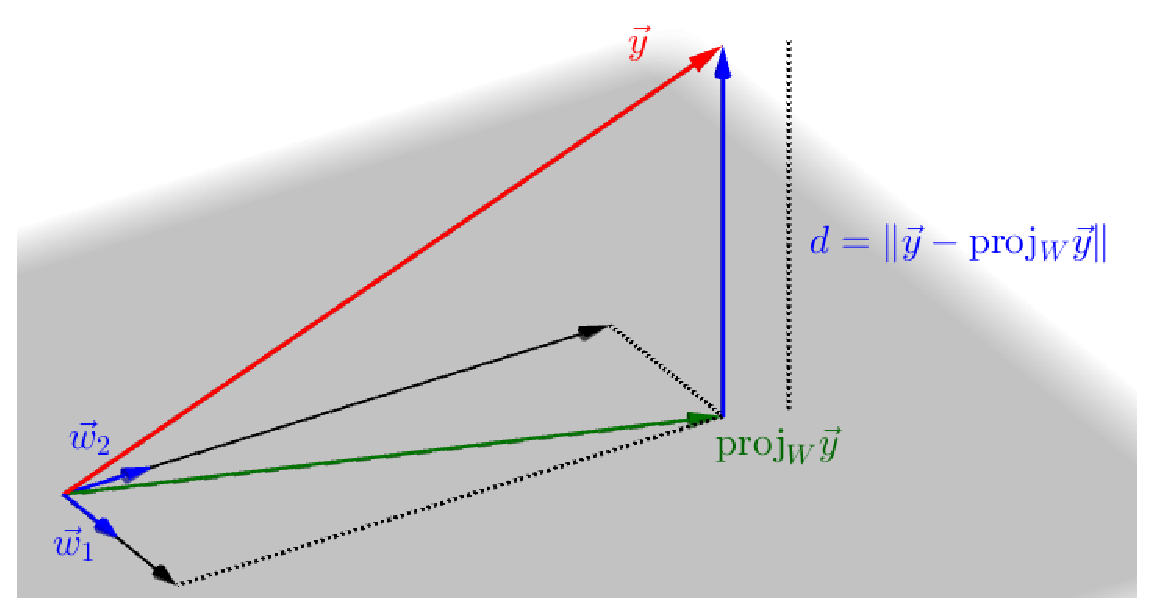
\includegraphics[width=1\linewidth]{Semana12/semana12-dist}
\end{center}
\end{figure}

\noindent Dado um ponto $P = (x_1, x_2, \dots, x_n)$, formamos o vetor da origem ao ponto $P$
\begin{equation}
\vec{y} = \vec{OP} =
\begin{bmatrix}
x_1 \\ x_2 \\ \vdots \\ x_n
\end{bmatrix}
\end{equation} cujas componentes são as coordenadas de $P$. Como vimos na seção anterior, o vetor $\vec{y} - \proj_{W} \vec{y}$ é ortogonal ao subespaço $W$. Sendo a distância de $P$ até $W$ denotada por $\operatorname{dist} (P,W)$ e definida como a menor distância entre $P$ e elementos de $W$, temos que
\begin{equation}
\operatorname{dist} (P,W) = \|\vec{y} - \proj_{W} \vec{y}\|.
\end{equation}


\begin{proof}[Justificativa desta afirmação]
Dado qualquer outro vetor $\vec{w} \in W$, o Teorema de Pitágoras implica que (ver figura)
\begin{equation}
\| \vec{y} - \vec{w} \|^2 = \| \vec{w} - \proj_{W} \vec{y}\|^2 + \| \vec{y} - \proj_{W} \vec{y}\|^2 > \| \vec{y} - \proj_{W} \vec{y}\|^2.
\end{equation} Em outras palavras, $\|\vec{y} - \proj_{W} \vec{y}\|$ é de fato a menor distância entre $P$ e elementos de $W$.
\begin{figure}[h!]
\begin{center}
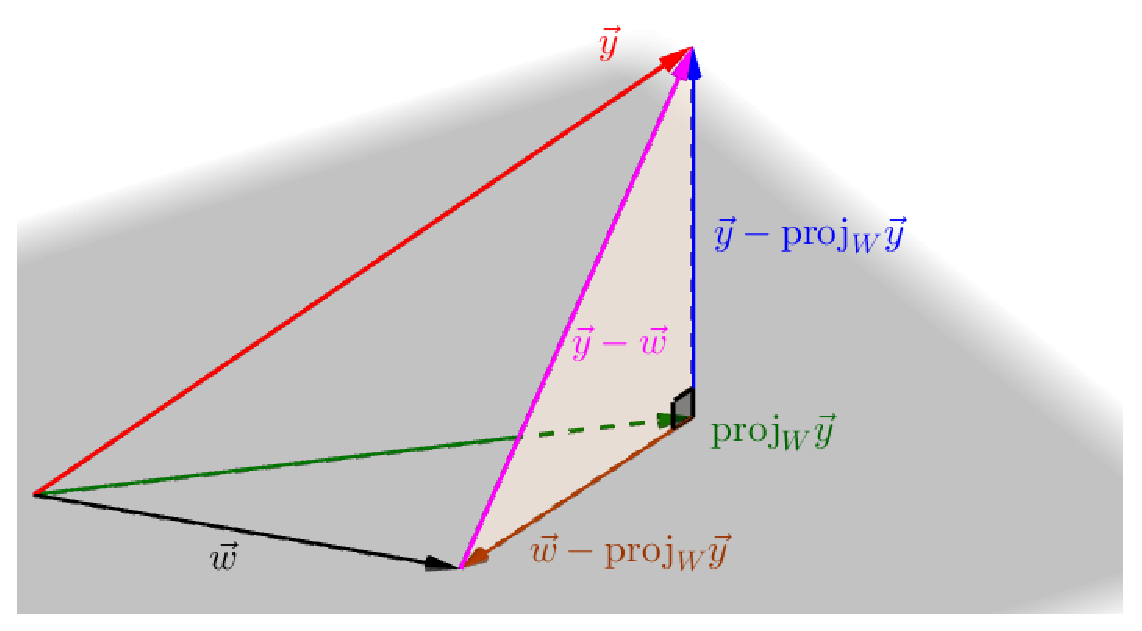
\includegraphics[width=1\linewidth]{Semana12/semana12-dist-justif}
\end{center}
\end{figure}
\end{proof}


\begin{ex}
Calcular a distância do ponto $P = (1,2,-1,0,7)$ até o plano $W = \Span\{\vec{u}, \vec{v}\}$ (contido em $\mathbb{R}^5$) gerado pelos vetores (que são ortogonais!)
\begin{equation}
\vec{u} =
\begin{bmatrix}
1 \\ 0 \\ -8 \\ 0 \\ 5
\end{bmatrix} \ \text{e} \ \
\vec{v} = \begin{bmatrix}
1 \\ -1 \\ 2 \\ 0 \\ 3
\end{bmatrix}.
\end{equation} Para isto, consideramos o vetor
\begin{equation}
\vec{y} = \vec{OP} = \begin{bmatrix}
1 \\ 2 \\ -1 \\ 0 \\ 7
\end{bmatrix}
\end{equation}e vamos calcular $\|\vec{y} - \proj_W \vec{y}\|$:
  \begin{align*}
\vec{y} - \proj_W \vec{y} & = \vec{y} - \frac{\vec{y} \cdot \vec{u}}{\vec{u} \cdot \vec{u}} \ \vec{u} - \frac{\vec{y} \cdot \vec{v}}{\vec{v} \cdot \vec{v}} \ \vec{v}  =
\begin{bmatrix}
1 \\ 2 \\ -1 \\ 0 \\ 7
\end{bmatrix} - \frac{44}{90}
\begin{bmatrix}
1 \\ 0 \\ -8 \\ 0 \\ 5
\end{bmatrix} - \frac{18}{15}
\begin{bmatrix}
1 \\ -1 \\ 2 \\ 0 \\ 3
\end{bmatrix} \\
   & = \begin{bmatrix}
1 \\ 2 \\ -1 \\ 0 \\ 7
\end{bmatrix} - \frac{22}{45}
\begin{bmatrix}
1 \\ 0 \\ 2 \\ 0 \\ 5
\end{bmatrix} - \frac{18}{15}
\begin{bmatrix}
1 \\ -1 \\ 2 \\ 0 \\ 3
\end{bmatrix} =
\begin{bmatrix}
-31/45 \\ 16/5 \\ -197/45 \\ 0 \\ 61/45
\end{bmatrix}
  \end{align*}
  Desta forma, a distância de $P$ a $W$ é
  \begin{align*}
\operatorname{dist} (P,W) & = \|\vec{y} - \proj_{W} \vec{y}\| = \sqrt{\frac{961}{2025} + \frac{256}{25} + \frac{38809}{2025} + \frac{3721}{2025}} = \sqrt{\frac{ 45795 }{2025}} \\
           & = \frac{ \sqrt{45795} }{45} \simeq 4,75. \ \lhd
  \end{align*}
\end{ex}




\section{O Processo de ortogonalização de Gram--Schmidt}

O \textbf{Processo de Gram--Schmidt} é um algoritmo para obter uma base ortogonal (ou ortonormal) a partir de uma base qualquer. De maneira mais geral, o método permite transformar um conjunto de vetores linearmente independentes em um conjunto ortogonal que gera o mesmo espaço vetorial.

Vamos começar com um exemplo.

\begin{ex}
Consideramos os vetores
\begin{equation}
\vec{v}_1 =
\begin{bmatrix}
1 \\ 0 \\ 1
\end{bmatrix}, \quad
\vec{v}_2 =
\begin{bmatrix}
1 \\ 1 \\ 0
\end{bmatrix} \quad \text{e} \quad
\vec{v}_3 =
\begin{bmatrix}
0 \\ 1 \\ 1
\end{bmatrix}.
\end{equation} O espaço gerado por $\{\vec{v}_1, \vec{v}_2, \vec{v}_3 \}$ é todo o espaço $\mathbb{R}^3$, já que temos três vetores  linearmente independentes em um espaço de dimensão três.

O processo consiste em fixar qualquer um dos vetores como o primeiro dos vetores do conjunto que virá a ser ortogonal. Por exemplo, fixamos
\begin{equation}
\vec{u}_1 = \vec{v}_1 =
\begin{bmatrix}
1 \\ 0 \\ 1
\end{bmatrix}.
\end{equation} Em seguida, já vimos que, ao fazer a projeção de $\vec{v}_2$ sobre $\vec{v}_1$, o vetor
\begin{equation}
\vec{v}_2 - \proj_{\vec{v}_1} \vec{v}_2
\end{equation} é ortogonal a $\vec{v}_1$, como ilustra a figura.
\begin{figure}[h!]
\begin{center}
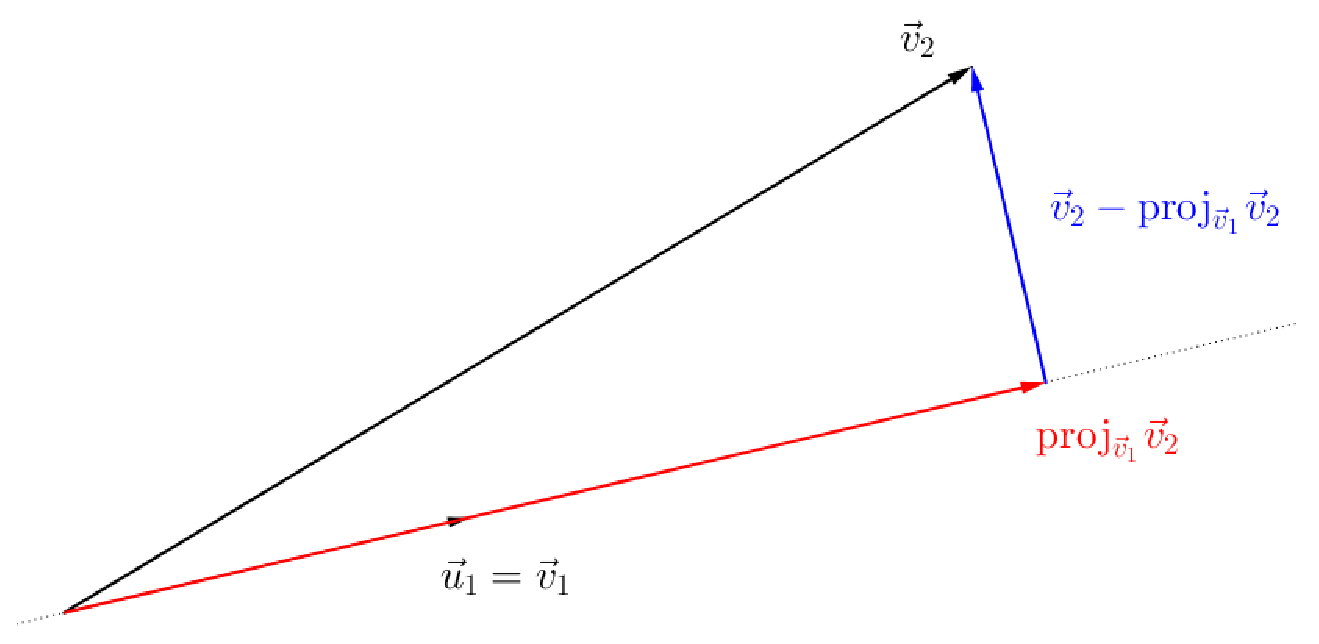
\includegraphics[width=0.7\linewidth]{Semana12/semana12-gram1}
\end{center}
\end{figure}

\noindent Assim sendo, definimos o segundo vetor do nosso conjunto que será ortogonal como o vetor
\begin{equation}
\vec{u}_2 = \vec{v}_2 - \proj_{\vec{u}_1} \vec{v}_2 = \vec{v}_2 - \frac{\vec{v}_2 \cdot \vec{u}_1}{\vec{u}_1 \cdot \vec{u}_1} \, \vec{u}_1 =
\begin{bmatrix}
1 \\ 1 \\ 0
\end{bmatrix}
- \frac{1}{2}
\begin{bmatrix}
1 \\ 0 \\ 1
\end{bmatrix} =
\begin{bmatrix}
1/2 \\ 1 \\ -1/2
\end{bmatrix} = \frac{1}{2}
\begin{bmatrix}
1 \\ 2 \\ -1
\end{bmatrix}.
\end{equation} Temos que $\vec{u}_1$ e $\vec{u}_2$ são ortogonais e que estão no mesmo plano, de modo que também temos
\begin{equation}
\Span \{ \vec{u}_1, \vec{u}_2 \} = \Span \{ \vec{v}_1, \vec{v}_2 \}.
\end{equation} Vamos escrever momentariamente $W = \Span \{ \vec{u}_1, \vec{u}_2 \}$.

No próximo passo do processo, o terceiro vetor pode ser obtido como
\begin{equation}
\vec{u}_3 = \vec{v}_3 - \proj_{W} \vec{v}_3,
\end{equation} pois, desta forma, $\vec{u}_3$ é ortogonal a todos os vetores de $W$; em particular, é ortogonal a ambos $\vec{u}_1$ e $\vec{u}_2$. Além disso, como $\vec{u}_1$ e $\vec{u}_2$ já são vetores ortogonais, podemos calcular a projeção sobre $W$ como de costume:
\begin{equation}
\vec{u}_3 = \vec{v}_3 - \proj_{W} \vec{v}_3 = \vec{v}_3 - \frac{\vec{v}_3 \cdot \vec{u}_1}{\vec{u}_1 \cdot \vec{u}_1} \, \vec{u}_1 - \frac{\vec{v}_3 \cdot \vec{u}_2}{\vec{u}_2 \cdot \vec{u}_2} \, \vec{u}_2.
\end{equation}
\begin{figure}[h!]
\begin{center}
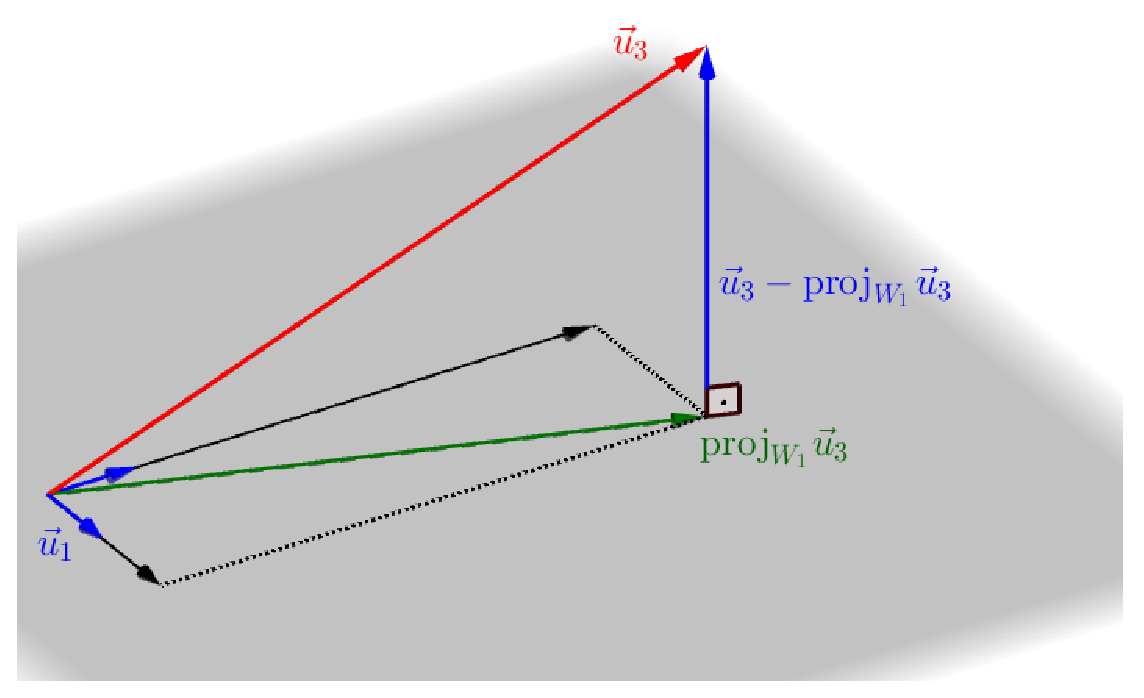
\includegraphics[width=0.9\linewidth]{Semana12/semana12-gram2}
\end{center}
\end{figure}

\noindent Calculando, temos (observe como dois fatores $1/2$ cancelam no último termo)
\begin{equation}
\vec{u}_3 =
\begin{bmatrix}
0 \\ 1 \\ 1
\end{bmatrix}  - \frac{1}{2}
\begin{bmatrix}
1 \\ 0 \\ 1
\end{bmatrix} - \frac{2 - 1}{1 + 4 +1}
\begin{bmatrix}
1 \\ 2 \\ -1
\end{bmatrix} =
\begin{bmatrix}
0 \\ 1 \\ 1
\end{bmatrix}  - \frac{1}{2}
\begin{bmatrix}
1 \\ 0 \\ 1
\end{bmatrix} - \frac{1}{6}
\begin{bmatrix}
1 \\ 2 \\ -1
\end{bmatrix} =
\begin{bmatrix}
-2/3 \\ 2/3 \\ 2/3
\end{bmatrix} = \frac{2}{3}
\begin{bmatrix}
-1 \\ 1 \\ 1
\end{bmatrix}
\end{equation} Concluimos assim que o conjunto
\begin{equation}
\{ \vec{u}_1, \vec{u}_2, \vec{u}_3 \} = \left\{
\begin{bmatrix}
1 \\ 0 \\ 1
\end{bmatrix},
\begin{bmatrix}
1/2 \\ 1 \\ -1/2
\end{bmatrix},
\begin{bmatrix}
-2/3 \\ 2/3 \\ 2/3
\end{bmatrix}  \right\}
\end{equation} é ortogonal e gera o mesmo espaço que $\{ \vec{v}_1, \vec{v}_2, \vec{v}_3 \}$.

Na realidade, se tivéssemos considerado múltiplos dos vetores acima, não perderíamos a propriedade de ortogonalidade, e temos
\begin{equation}
\Span \{ \vec{u}_1, \vec{u}_2, \vec{u}_3 \} =
\Span \left\{
\begin{bmatrix}
1 \\ 0 \\ 1
\end{bmatrix},
\begin{bmatrix}
1 \\ 2 \\ -1
\end{bmatrix},
\begin{bmatrix}
-1 \\ 1 \\ 1
\end{bmatrix}
\right\}.
\end{equation} ``Colocar em evidência'' os fatores comuns desta forma e ``desconsiderá-los'' pode facilitar as contas em alguns casos.

Observamos também que, fazendo a normalização dos vetores, podemos obter uma base ortonormal:
\begin{equation}
\left\{
  \begin{array}{ll}
   \|\vec{u}\| = \sqrt{1 + 0 + 1} = \sqrt{2} \\
   \|\vec{v}\| = \sqrt{1 + 4 + 1} = \sqrt{6} \\
   \|\vec{w}\| = \sqrt{1 + 1 + 1} = \sqrt{3} \\
  \end{array}
\right.
\end{equation} e assim,
\begin{equation}
\frac{\vec{u}_1}{\|\vec{u}_1\|} = \frac{1}{\sqrt{3}}
\begin{bmatrix}
1 \\ 0 \\ 1
\end{bmatrix} =
\begin{bmatrix}
1/\sqrt{2} \\ 0 \\ 1/\sqrt{2}
\end{bmatrix}, \
\frac{\vec{u}_2}{\|\vec{u}_2\|} = \frac{1}{\sqrt{6}}
\begin{bmatrix}
1 \\ 2 \\ -1
\end{bmatrix} =
\begin{bmatrix}
1/\sqrt{6} \\ 2/\sqrt{6} \\ -1/\sqrt{6}
\end{bmatrix} \ \text{e }
\frac{\vec{u}_3}{\|\vec{u}_3\|} = \frac{1}{\sqrt{3}}
\begin{bmatrix}
-1 \\ 1 \\ 1
\end{bmatrix} =
\begin{bmatrix}
-1/\sqrt{3} \\ 1/\sqrt{3} \\ 1/\sqrt{3}
\end{bmatrix}
\end{equation} forma um conjunto ortonormal que gera o mesmo espaço vetorial que $\{ \vec{v}_1, \vec{v}_2, \vec{v}_3 \}. \ \lhd$
\end{ex}



Em seguida, mostramos como funciona o processo de maneira geral (um bom entendimento do exemplo acima deve deixar claro o porquê deste processo funcionar): sejam $k$ vetores linearmente independentes $\vec{v}_1, \vec{v}_2, \cdots, \vec{v}_k$ pertencentes ao espaço $n$-dimensional $\mathbb{R}^n$. Vamos denotar
\begin{equation}
W = \Span \{\vec{v}_1, \vec{v}_2, \cdots, \vec{v}_k\}
\end{equation} e construir uma base ortogonal (e em seguida ortonormal) para $W$. Começamos com
\begin{equation}
\boxed{\vec{u}_1 = \vec{v}_1}
\end{equation} e definimos
\begin{equation}\label{eqn:Gram-Schmidt-1}
\boxed{\vec{u}_2 = \vec{v}_2 - \proj_{\vec{u}_1} \vec{v}_2 = \vec{v}_2 - \frac{\vec{v}_2 \cdot \vec{u}_1}{\vec{u}_1 \cdot \vec{u}_1} \, \vec{u}_1.}
\end{equation}
 Temos que $\vec{u}_1$ e $\vec{u}_2$ são ortogonais e que estão no mesmo plano, de modo que também temos
\begin{equation}
\Span \{ \vec{u}_1, \vec{u}_2 \} = \Span \{ \vec{v}_1, \vec{v}_2 \} = W_2 \ \leftrightsquigarrow \text{ notação.}
\end{equation} Em seguida, definimos
\begin{equation}\label{eqn:Gram-Schmidt-2}
\boxed{\vec{u}_3 = \vec{v}_3 - \proj_{W_2} \vec{v}_3 = \vec{v}_3 - \frac{\vec{v}_3 \cdot \vec{u}_1}{\vec{u}_1 \cdot \vec{u}_1} \, \vec{u}_1 - \frac{\vec{v}_3 \cdot \vec{u}_2}{\vec{u}_2 \cdot \vec{u}_2} \, \vec{u}_2.}
\end{equation} Temos que $\vec{u}_1, \vec{u}_2, \vec{u}_3$ ortogonais e
\begin{equation}
\Span \{ \vec{u}_1, \vec{u}_2, \vec{u}_3 \} = \Span \{ \vec{v}_1, \vec{v}_2, \vec{v}_3 \} = W_3 \ \leftrightsquigarrow \text{ notação.}
\end{equation} Em seguida
\begin{equation}
\boxed{\vec{u}_4 = \vec{v}_4 - \proj_{W_3} \vec{v}_4 = \vec{v}_4 - \frac{\vec{v}_4 \cdot \vec{u}_1}{\vec{u}_1 \cdot \vec{u}_1} \, \vec{u}_1 - \frac{\vec{v}_4 \cdot \vec{u}_2}{\vec{u}_2 \cdot \vec{u}_2} \, \vec{u}_2 - \frac{\vec{v}_4 \cdot \vec{u}_3}{\vec{u}_3 \cdot \vec{u}_3} \, \vec{u}_3.}
\end{equation} Temos que $\vec{u}_1, \vec{u}_2, \vec{u}_3, \vec{u}_4$ ortogonais e
\begin{equation}
\Span \{ \vec{u}_1, \vec{u}_2, \vec{u}_3, \vec{u}_4 \} = \Span \{ \vec{v}_1, \vec{v}_2, \vec{v}_3, \vec{u}_4 \} = W_4 \ \leftrightsquigarrow \text{ notação.}
\end{equation} E assim seguimos fazendo as contas até chegar ao último vetor: sendo
\begin{equation}
\Span \{ \vec{u}_1, \vec{u}_2, \cdots, \vec{u}_{k-1} \} = \Span \{ \vec{v}_1, \vec{v}_2, \cdots, \vec{v}_{k-1} \} = W_{k-1} \ \leftrightsquigarrow \text{ notação,}
\end{equation} escrevemos
\begin{equation}
\boxed{\vec{u}_k = \vec{v}_k - \proj_{W_{k-1}} \vec{v}_k = \vec{v}_k - \frac{\vec{v}_k \cdot \vec{u}_1}{\vec{u}_1 \cdot \vec{u}_1} \, \vec{u}_1 - \frac{\vec{v}_k \cdot \vec{u}_2}{\vec{u}_2 \cdot \vec{u}_2} \, \vec{u}_2 - \cdots - \frac{\vec{v}_k \cdot \vec{u}_{k-1}}{\vec{u}_{k-1} \cdot \vec{u}_{k-1}} \, \vec{u}_{k-1}.}
\end{equation} Temos que $\{\vec{u}_1, \vec{u}_2, \dots, \vec{u}_k\}$ é um conjunto ortogonal e
\begin{equation}
\Span \{ \vec{u}_1, \vec{u}_2, \dots, \vec{u}_k \} = \Span \{ \vec{v}_1, \vec{v}_2, \dots, \vec{u}_k \} = W \ \leftrightsquigarrow \text{ que é o espaço inicial, }
\end{equation} como queríamos.

Esta parte (obter o conjunto ortogonal) é a mais ``pesada'' do método. Por exemplo, se agora quiséssemos uma base ortonormal para $W$, basta considerar o conjunto
\begin{equation}
\left\{ \frac{\vec{u}_1}{\|\vec{u}_1\|}, \frac{\vec{u}_2}{\|\vec{u}_2\|}, \dots, \frac{\vec{u}_k}{\|\vec{u}_k\|} \right\},
\end{equation} que continua sendo ortogonal, mas agora formado por vetores unitários.




\begin{ex}\footnote{A matriz $A$ deste exemplo foi retirada de Wikipedia.org \href{https://en.wikipedia.org/w/index.php?title=QR_decomposition&oldid=810854220}{neste} link permanente, em 21 de Novembro de 2017.}
Vamos obter uma base ortonormal para o espaço coluna $\operatorname{Col} A$ da matriz
\begin{equation}
A =
\begin{bmatrix}
12 & -51 & 4 \\
6 & 167 & -68 \\
-4 & 24 & -41
\end{bmatrix}.
\end{equation} Lembrando que $\operatorname{Col} A$ é o espaço gerado pelas colunas de $A$ (e observando que, neste caso, $\dim \operatorname{Col} A = 3$), vamos aplicar o processo de Gram--Schmidt para os vetores
\begin{equation}
\vec{v}_1 =
\begin{bmatrix}
12 \\
6 \\
-4
\end{bmatrix},
\vec{v}_2 =
\begin{bmatrix}
 -51  \\
 167  \\
 24
\end{bmatrix} \ \text{ e } \ \vec{v}_3 =
\begin{bmatrix}
  4 \\
 -68 \\
 -41
\end{bmatrix}.
\end{equation} O processo começa como:
\begin{align*}
\vec{u}_1 & = \vec{v}_1 =
\begin{bmatrix}
12 \\
6 \\
-4
\end{bmatrix}, \\
\vec{u}_2 &  = \vec{v}_2 - \frac{\vec{v}_2 \cdot \vec{u}_1}{\vec{u}_1 \cdot \vec{u}_1} \, \vec{u}_1 =
\begin{bmatrix}
 -51  \\
 167  \\
 24
\end{bmatrix} - \frac{-612 +1002 - 96}{144 + 36 + 16}
\begin{bmatrix}
12 \\
6 \\
-4
\end{bmatrix}\\
& =
\begin{bmatrix}
 -51  \\
 167  \\
 24
\end{bmatrix} - \frac{296}{196}
\begin{bmatrix}
12 \\
6 \\
-4
\end{bmatrix} =
\begin{bmatrix}
 -69  \\
 158  \\
 30
\end{bmatrix}
  \end{align*}
 Em seguida (conferir estas contas com o auxílio de uma calculadora)
  \begin{align*}
\vec{u}_3 & = \vec{v}_3 - \frac{\vec{v}_3 \cdot \vec{u}_1}{\vec{u}_1 \cdot \vec{u}_1} \, \vec{u}_1 - \frac{\vec{v}_3 \cdot \vec{u}_2}{\vec{u}_2 \cdot \vec{u}_2} \, \vec{u}_2 \\
& = \begin{bmatrix}
  4 \\
 -68 \\
 -41
\end{bmatrix} - \frac{48-408 + 164}{196}
\begin{bmatrix}
12 \\
6 \\
-4
\end{bmatrix} - \frac{-276 - 10744 - 1230}{4761 + 24694 + 900}
\begin{bmatrix}
 -69  \\
 158  \\
 30
\end{bmatrix} \\
   & = \begin{bmatrix}
  4 \\
 -68 \\
 -41
\end{bmatrix} + \cancel{\frac{196}{196}}
\begin{bmatrix}
12 \\
6 \\
-4
\end{bmatrix} + \frac{12250}{30355}
\begin{bmatrix}
 -69  \\
 158  \\
 30
\end{bmatrix} = \begin{bmatrix}
 -58/5  \\
 6/5  \\
 -33
\end{bmatrix}.
  \end{align*}
  Para obter uma base ortonormal para o espaço coluna, vamos ainda considerar
\begin{equation}
\frac{\vec{u}_1}{\|\vec{u}_1\|}, \frac{\vec{u}_2}{\|\vec{u}_2\|}, \frac{\vec{u}_3}{\|\vec{u}_3\|}.
\end{equation} Calculamos
\begin{equation}
\left\{
  \begin{array}{ll}
   \|\vec{u}_1\| = \sqrt{196} = 14 \\
   \|\vec{u}_2\| = \sqrt{30625} = 175 \\
   \|\vec{u}_3\| = \frac{\sqrt{30625}}{5} = 35
  \end{array}
\right.
\end{equation} Portanto, uma base ortonormal para $\operatorname{Col} A$ é
\begin{equation}
\vec{n}_1 = \frac{\vec{u}_1}{\|\vec{u}_1\|} =
\begin{bmatrix}
 6/7  \\
 3/7  \\
 -2/7
\end{bmatrix}, \quad
\vec{n}_2 = \frac{\vec{u}_2}{\|\vec{u}_2\|} =
\begin{bmatrix}
 -69/175  \\
 158/175  \\
 6/35
\end{bmatrix} \quad \text{e} \quad
\vec{n}_3 = \frac{\vec{u}_3}{\|\vec{u}_3\|} =
\begin{bmatrix}
 -58/175  \\
 6/175  \\
 -33/35
\end{bmatrix}. \lhd
\end{equation}
\end{ex}


\section{Fatoração QR e matrizes ortogonais}


Como passamos a discutir abaixo, o método de Gram-Schmidt permite fatorar uma matriz $A$ cujas colunas são linearmente independentes em um produto \begin{equation}A=QR,\end{equation} onde Q é uma matriz cujas colunas formam um conjunto ortonormal e $R$ é uma matriz triangular superior. Tal fatoração é muito importante do ponto de vista computacional, como veremos em breve, quando usarmos a fatoração QR como uma alternativa para resolução de sistemas lineares por mínimos quadrados. Também é a base de um eficiente método numérico para encontrar autovalores de uma matriz quadrada.

Matrizes cujas colunas formam um conjunto ortonormal são muito úteis e por isso recebem um nome especial: são chamadas de \textbf{matrizes ortogonais}. Aqui cabe uma observação relevante: este é um exemplo de uma situação onde a terminologia clássica está longe de ser satisfatória: matrizes  cujas colunas formam um conjunto {\it ortonormal} são chamadas de matrizes {\it ortogonais}.

\medskip

Faremos agora uma exposição da fatoração QR usando uma matriz inicial $A$ que tem 3 colunas, observando que a construção abaixo é facilmente generalizada para uma matriz de qualquer dimensão (desde que tenha colunas LI).

Dada uma matriz $A=\begin{bmatrix}
\vec{v}_1 & \vec{v}_2 & \vec{v}_3
\end{bmatrix}$ cujas colunas são LI e são denotadas pelos vetores $\vec{v}_1$, $\vec{v}_2$, e $\vec{v}_3$,
o processo de Gram-Schmidt começa com a construção de uma base ortogonal formada pelos vetores
$\vec{u}_1$, $\vec{u}_2$, e $\vec{u}_3$,
para o espaço-coluna da matriz $A$. Para isso, definimos

\begin{equation}
\begin{cases}
\vec{u}_1 = \vec{v}_1 \\
\vec{u}_2 = \vec{v}_2 - \proj_{\vec{u}_1} \vec{v}_2 \\
\vec{u}_3 = \vec{v}_3 - \proj_{\Span\{\vec{u}_1,\vec{u}_2\}} \vec{v}_3
\end{cases}
\end{equation}
Desta forma, existem coeficientes $b_1$, $c_1$ e $c_2 \in \mathbb{R}$ tais que
\begin{equation}
\begin{cases}
\vec{u}_1 = \vec{v}_1 \\
\vec{u}_2 = \vec{v}_2 - b_1 \vec{u}_1 \\
\vec{u}_3 = \vec{v}_3 - c_1 \vec{u}_1 - c_2 \vec{u}_2
\end{cases}.
\end{equation} Estes coeficientes são justamente aqueles que aparecem nas fórmulas \eqref{eqn:Gram-Schmidt-1} e \eqref{eqn:Gram-Schmidt-2}. Apenas denotamos desta forma para não poluir as equações e facilitar o entendimento.

Em um segundo momento, cada um dos três vetores $\vec{u}_1$, $\vec{u}_2$, e $\vec{u}_3$ pode ser normalizado, ou seja, podemos dividir cada um deles pelo seu comprimento para obter uma base ortonormal. Assim, $\vec{u}_1$, $\vec{u}_2$, e $\vec{u}_3$ formam uma base ortonormal para o espaço coluna de $A$, e existem coeficientes $\alpha_1$, $\beta_1$, $\beta_2$, $\gamma_1$, $\gamma_2$ e $\gamma_3 \in \mathbb{R}$ tais que\footnote{Para simplificar a notação, continuamos escrevendo $\vec{u}_i$ quando, na realidade, deveríamos escrever $\vec{u}_i/\|\vec{u}_i\|$. Observe também que cada um dos coeficientes é obtido simplesmente pela normalização dos vetores. Mais explicitamente, temos
\begin{equation}
\alpha_1 = \frac{1}{\|\vec{u}_1\|}, \quad \beta_2 = \frac{1}{\|\vec{u}_2\|}, \quad \beta_1 = \frac{b_1}{\|\vec{u}_2\|}, \quad \gamma_3 = \frac{1}{\|\vec{u}_3\|}, \quad \gamma_1 = \frac{c_1}{\|\vec{u}_3\|} \quad \text{e} \quad \gamma_2 = \frac{c_2}{\|\vec{u}_3\|}.
\end{equation}}
\begin{equation}
\begin{cases}
\vec{u}_1 = \alpha_1\vec{v}_1 \\
\vec{u}_2 = \beta_2 \vec{v}_2 - \beta_1 \vec{u}_1 \\
\vec{u}_3 = \gamma_3 \vec{v}_3 - \gamma_1 \vec{u}_1 - \gamma_2 \vec{u}_2
\end{cases}
\end{equation}


Podemos agora inverter estas equações (que são do tipo triangular -- faça as contas!) para escrever as colunas da matriz $A$ em função dos vetores da base ortonormal $\{\vec{u}_1, \vec{u}_2, \vec{u}_3\}$ que acaba de ser obtida:
\begin{equation}
\begin{cases}
\vec{v}_1 = \alpha_1^{-1}\vec{u}_1 \\
\vec{v}_2 = \beta_2^{-1}\beta_1 \vec{u}_1 + \beta_2^{-1} \vec{u}_2 \\
\vec{v}_3 =  \gamma_3^{-1}\gamma_1 \vec{u}_1 +  \gamma_3^{-1}\gamma_2 \vec{u}_2 + \gamma_3^{-1} \vec{u}_3
\end{cases}
\end{equation} Matricialemente, estas equações podem ser escritas como
\begin{equation}
\begin{bmatrix}
| & | & | \\
\vec{v}_1  & \vec{v}_2 & \vec{v}_3\\
| & | & | \\
\end{bmatrix} =
\begin{bmatrix}
| & | & | \\
\vec{u}_1  & \vec{u}_2 & \vec{u}_3 \\
| & | & | \\
\end{bmatrix}
\begin{bmatrix}
\alpha_1^{-1}  & \beta_2^{-1}\beta_1  & \gamma_3^{-1}\gamma_1 \\
0 & \beta_2^{-1} & \gamma_3^{-1}\gamma_2 \\
0 & 0 & \gamma_3^{-1}
\end{bmatrix},
\end{equation} visto que cada coluna do produto da direita é definido como a combinação linear das colunas da primeira matriz com pesos dados pela respectiva coluna da segunda matriz.\footnote{Comparar, por exemplo, com as Subseções \ref{scn:resolucao-2-sistemas} e \ref{scn:alg-ordem-maior}, onde este tipo de interpretação para o produto de matrizes foi discutido.}
Assim, definindo
\begin{equation}
Q=\begin{bmatrix}
| & | & | \\
\vec{u}_1 & \vec{u}_2 & \vec{u}_3 \\
| & | & | \\
\end{bmatrix} \quad \text{e} \quad
R =
\begin{bmatrix}
\alpha_1^{-1}  & \beta_2^{-1}\beta_1  & \gamma_3^{-1}\gamma_1 \\
0 & \beta_2^{-1} & \gamma_3^{-1}\gamma_2 \\
0 & 0 & \gamma_3^{-1}
\end{bmatrix},
\end{equation} obtemos
\begin{equation}
A=QR,
\end{equation} que é o que queríamos obter.

Note também que $R$ é invertível, já que sua diagonal principal contém apenas termos não-nulos.

A construção acima é facilmente generalizada para matrizes quaisquer e nos permite enunciar o seguinte fato
(lembre que uma matriz ortogonal é uma matriz cujas colunas formam um conjunto ortonormal):

\begin{teo}
Qualquer matriz $A$ cujas colunas são linearmente independentes pode ser fatorada na forma $A=QR$, onde $Q$ é uma matriz ortogonal
e $R$ é uma matriz triangular superior invertível. Ainda, o espaço coluna das matrizes $A$ e $Q$ é o mesmo, ou seja, as colunas de $Q$ formam uma base ortonormal para o subespaço gerado pelas colunas de $A$.
\end{teo}

Note que a fatoração QR está para o processo de Gram-Schmidt assim como a fatoração LU está para o método de  eliminação gaussiana à forma escada  %\footnote{Preciso escrever sobre a fatoração LU. Acho que seria interessante também mostrar que matrizes ortogonais preservam comprimento e ângulo.}

Bem, vimos que a matriz $Q$ tem como colunas a base ortonormal gerada pelo processo de Gram-Schmidt. E como podemos calcular a matriz $R$ no caso geral ?

Usando o seguinte fato surpreendente:

\begin{teo}
Uma matriz ortogonal é sempre invertível e sua inversa é dada pela sua transposta, ou seja $Q^{-1}= Q^T$.
\end{teo}

\begin{proof}
A prova deste teorema é uma simples verificação:
\begin{equation}
Q^T Q =
\begin{bmatrix}
\text{ --- }\  \vec{u}_1 \, \text{ --- } \\
\text{ --- }\  \vec{u}_2 \, \text{ --- } \\
\text{ --- }\  \vec{u}_3 \, \text{ --- }
\end{bmatrix}
\begin{bmatrix}
| & | & | \\
\vec{u}_1 & \vec{u}_2 & \vec{u}_3 \\
| & | & |
\end{bmatrix} =
\begin{bmatrix}
\vec{u}_1 \cdot \vec{u}_1 & \vec{u}_1 \cdot \vec{u}_2 & \vec{u}_1 \cdot \vec{u}_2 \\
\vec{u}_2 \cdot \vec{u}_1 & \vec{u}_2 \cdot \vec{u}_2 & \vec{u}_2 \cdot \vec{u}_3 \\
\vec{u}_3 \cdot \vec{u}_1 & \vec{u}_3 \cdot \vec{u}_2 & \vec{u}_3 \cdot \vec{u}_3
\end{bmatrix} =
\begin{bmatrix}
1 & 0 & 0 \\
0 & 1 & 0 \\
0 & 0 & 1
\end{bmatrix} = I. \qedhere
\end{equation}
\end{proof}


Assim, se $A=QR$, basta multiplicar ambos os lados desta equação por $Q^T$ pela esquerda para obtermos:

\begin{equation}Q^T A = Q^T Q R \ \Longrightarrow \ R= Q^T A.\end{equation}






\vspace{0.3cm}



No último exemplo da seção anterior, obtemos através do método de Gram-Schmidt uma base ortonormal para $\operatorname{Col} A$
onde
\begin{equation}
A =
\begin{bmatrix}
12 & -51 & 4 \\
6 & 167 & -68 \\
-4 & 24 & -41
\end{bmatrix}.
\end{equation}
Vamos definir a matriz $Q$ como a matriz formada pelos vetores desta base ortonormal:
\begin{equation}
Q =
\begin{bmatrix}
6/7 & -69/175 & -58/175 \\
3/7 & 158/175 & 6/175   \\
-2/7& 6/35   &-33/35
\end{bmatrix}
\end{equation}

%tem, portanto, suas colunas ortonormais.
%É possível verificar que ao fazermos $Q^T A$ obtemos uma matriz triangular $R$. Podemos escrever
Vimos que $R=Q^T A$ e portanto
\begin{equation}
R = Q^T A =
\begin{bmatrix}
6/7 & 3/7 & -2/7 \\
-69/175 & 158/175 & 6/35   \\
-58/175& 6/175   &-33/35
\end{bmatrix}
\begin{bmatrix}
12 & -51 & 4 \\
6 & 167 & -68 \\
-4 & 24 & -41
\end{bmatrix} =
\begin{bmatrix}
14&21&-14\\
0&175&-70\\
0&0&35
\end{bmatrix} .
\end{equation}
Finalmente podemos escrever
\begin{equation}
A =
\begin{bmatrix}
12 & -51 & 4 \\
6 & 167 & -68 \\
-4 & 24 & -41
\end{bmatrix} =
\begin{bmatrix}
6/7 & -69/175 & -58/175 \\
3/7 & 158/175 & 6/175   \\
-2/7& 6/35   &-33/35
\end{bmatrix}
\begin{bmatrix}
14&21&-14\\
0&175&-70\\
0&0&35
\end{bmatrix} = QR. \ \lhd
\end{equation}


\section{Matrizes Ortogonais preservam comprimento e ângulo}

Vamos aproveitar para falar um pouco mais sobre matrizes ortogonais. Um exemplo clássico de matriz ortogonal de ordem $2\times 2$ é dada pela matriz de rotação (esta no sentido anti-horário, ver Exemplo \ref{exp:rotacao})
\begin{equation}
Q =
\begin{bmatrix}
\cos \theta & -\sen \theta \\
\sen \theta & \cos \theta
\end{bmatrix} ,\end{equation}
onde $0 \leq \theta \leq 2 \pi$.
Podemos ver que esta matriz define uma transformação linear no plano que rotaciona vetores em um ângulo $\theta$ no sentido anti-horário.
Assim, tal transformação preserva comprimento e ângulo entre vetores.
Estas propriedades não são particulares da matriz de rotação: todas as matrizes ortogonais se comportam da mesma forma. O teorema a seguir traz estas informações e mais algumas.

\begin{teo}
	Seja $Q= \begin{bmatrix}
	\vec{u}_1 & \vec{u}_2 & \cdots & \vec{u}_n
	\end{bmatrix}$ uma matriz ortogonal de ordem $n \times n$. Então, para quaisquer vetores $\vec{v}$ e $\vec{w}$ em $\mathbb{R}^n$ temos
	\begin{enumerate}[$(i)$]
		\item $Q\vec{v} \cdot Q\vec{w} = \vec{v} \cdot  \vec{w}$
		\item  $\| Q\vec{v} \| = \| \vec{v} \|$
		\item  o ângulo entre $Q\vec{v}$ e $Q\vec{w}$ é igual ao  ângulo entre $\vec{v}$ e $\vec{w}$
		\end{enumerate}
\end{teo}

\begin{proof}
A prova do primeiro item é consequência direta da linearidade do produto interno e da hipótese das colunas formarem uma base ortonormal: se, na base canônica, temos $\vec{v} = (\alpha_1,..., \alpha_n)$ e $\vec{w} = (\beta_1, ..., \beta_n)$, então
\begin{equation}Q\vec{v} \cdot Q\vec{w} = \left( \sum_{i=1}^n \alpha_i \vec{u}_i \right) \cdot \left(   \sum_{j=1}^n \beta_j \vec{u}_j \right) =  \sum_{i=1}^n \sum_{j=1}^n \alpha_i \beta_j \;\vec{u}_i \cdot \vec{u}_j\end{equation}
devido a linearidade do produto interno (ou seja, a propriedade distributiva aplicada tanto na primeira quanto na segunda componente do produto interno). Agora, lembrando que $\vec{u}_i \cdot \vec{u}_j=0$ se $i \neq j$, a ultima expressão iguala-se a
\begin{equation} \sum_{i=1}^n \alpha_i \beta_i \; \vec{u}_i \cdot \vec{u}_i.\end{equation}
Finalmente, lembrando que cada coluna $\vec{u}_i$ de $Q$ tem comprimento unitário, concluimos que
\begin{equation}Q\vec{v} \cdot Q\vec{w} = \sum_{i=1}^n \alpha_i \beta_i = \vec{v} \cdot \vec{w}.\end{equation}


 Os próximos dois itens seguem diretamente do primeiro item, visto que
\begin{equation}\| Q \vec{v} \| = \sqrt{Q\vec{v} \cdot Q\vec{v}} = \sqrt{\vec{v} \cdot \vec{v}} =  \| \vec{v} \| \end{equation}
e
o ângulo entre $Qv$ e $Qw$ é definido como
\begin{equation}
\arccos\left(\frac{Qv \cdot Qw	}{\|Qv\| \|Qw\|} \right)
=\arccos\left(\frac{v \cdot w	}{\|v\| \|w\|} \right),\end{equation}
que por definição é o ângulo  entre $v$ e $w$.
Assim, finalizamos a prova do teorema.
\end{proof}


% \medskip


Outros exemplos de matrizes ortogonais são obtidos por matrizes de reflexão. Um caso particular é dado pela reflexão em torno do eixo horizontal:
 \begin{equation}
 Q =
 \begin{bmatrix}
 1 & 0 \\
 0 & -1
 \end{bmatrix}.\end{equation}

 \begin{exer}
Como é a matriz de ordem $2 \times 2$ que representa uma reflexão com respeito ao eixo vertical?
 \end{exer}

 \begin{exer}
Encontrar uma matriz de ordem $2 \times 2$ que representa uma reflexão com respeito à reta que passa pela origem de equação $ax + b y = 0$.
\end{exer}

%\end{document}







\include{Semana13/semana13-LLScomQR}
% Este trabalho está licenciado sob a Licença Creative Commons Atribuição-CompartilhaIgual 3.0 Não Adaptada. Para ver uma cópia desta licença, visite https://creativecommons.org/licenses/by-sa/3.0/ ou envie uma carta para Creative Commons, PO Box 1866, Mountain View, CA 94042, USA.

%\documentclass[../livro.tex]{subfiles}

\providecommand{\dir}{..}  %define o diretório principal

%\begin{document}

\chapter{Semanas 14 e 15}

\section{Matrizes simétricas}

Uma \textbf{matriz simétrica} é uma matriz que é igual à sua transposta. Para que esta definição faça sentido, apenas podemos considerar matrizes que são quadradas. De forma mais precisa, se $A = \begin{bmatrix} a_{ij} \end{bmatrix}$ é uma matriz de orden $n \times n$, nós dizemos que $A$ é simétrica quando $A = A^T$.

Formas equivalentes de dizer que $A$ é simétrica incluem:
\begin{enumerate}[$(1)$]
	\item $A = A^T$;
	\item para todos os índices $i,j \in \{1,2,\dots,n\}$, temos que $a_{ij} = a_{ji}$;
	\item as colunas de $A$ são iguais às linhas de $A^T$;
	\item as linhas de $A$ são iguais às colunas de $A^T$.
\end{enumerate}

\begin{ex}
	As matrizes
	\begin{equation}
	\begin{bmatrix}
	1 & -3 \\
	-3 &  2
	\end{bmatrix}, \ \ 
	\begin{bmatrix}
	1 & -3 \\
	-3 &  1
	\end{bmatrix}, \ \ 
	\begin{bmatrix}
	1 & -3 & 0 \\
	-3 & -1 & 4 \\
	0 &  4 & 6
	\end{bmatrix} \checkmark
	\end{equation} são simétricas, enquanto  as matrizes
	\begin{equation}
	\begin{bmatrix}
	1 & -3 \\
	3 &  1
	\end{bmatrix},\ \ 
	\begin{bmatrix}
	1 &  3 \\
	-3 &  2
	\end{bmatrix},\ \ 
	\begin{bmatrix}
	1 & -3 &  0 \\
	4 & -1 & -3 \\
	0 &  4 &  1
	\end{bmatrix} \textsc{x}
	\end{equation} não são. Deve-se tomar o cuidado de verificar a simetria \textit{com relação à diagonal principal}. Qualquer outro tipo de simetria não deve interferir na nossa análise$. \ \lhd$
\end{ex}

Um dos resultados mais importantes de Álgebra Linear é o Teorema Espectral, que diz que toda matriz simétrica é diagonalizável por uma base de autovetores que é ortonormal. De forma mais precisa:

\begin{teoespectral}
	Suponhamos que $A$ é uma matriz simétrica com coeficientes reais. Então:
	\begin{enumerate}[$(i)$]
		\item todos os autovalores de $A$ são reais;
		\item autovetores associados a autovalores distintos são ortogonais.
		\item a dimensão do autoespaço associado a um autovalor é igual à multiplicidade deste autovalor como raiz do polinômio característico;
		\item existe uma base ortonormal de $\mathbb{R}^n$ formada por autovetores de $A$;
		\item $A$ é diagonalizável por uma matriz de mudança de coordenadas ortonormal $P$: a matriz $P$ cujas colunas são os autovetores (ortonormais) de $A$ é tal que 
		\begin{equation}
		P^{T} A P = P^{-1} A P = D.
		\end{equation}
	\end{enumerate}
\end{teoespectral}

Nós vamos apresentar uma prova deste resultado no final destas notas. Antes de mais nada, faremos alguns exemplos e aplicações que justificam a importância do Teorema Espectral. No entanto, é fortemente aconselhado que o leitor acompanhe os elementos da demonstração, para efetivamente entender as propriedades essenciais das matrizes simétricas.

\begin{ex}
	Considere
	\begin{equation}
	A = \begin{bmatrix}
	1 & -5 \\
	-5 &  1
	\end{bmatrix}.
	\end{equation} O polinômio característico é
	\begin{equation}
	\det \begin{bmatrix}
	1-\lambda & -4 \\
	-4 & 5-\lambda
	\end{bmatrix} = (1-\lambda)^2 - 25 = \lambda^2 - 2 \lambda - 24
	\end{equation} cujas raízes são $6$ e  $-4$. Os autovetores são calculados como
	\begin{equation}
	A + 4 I = 
	\begin{bmatrix}
	5 & -5 \\
	-5 & 5
	\end{bmatrix} \sim 
	\begin{bmatrix}
	1 & -1 \\
	0 & 0
	\end{bmatrix} \implies 
	\left\{
	\begin{array}{l}
	v_1 = v_2 \\ 
	\text{uma variável livre}
	\end{array}
	\right. \implies \vec{v}_1 = v_2
	\begin{bmatrix}
	1  \\
	1
	\end{bmatrix}.
	\end{equation} Associado com $6$:
	\begin{equation}
	A - 6 I = 
	\begin{bmatrix}
	-5 & -5 \\
	-5 & -5
	\end{bmatrix} \sim 
	\begin{bmatrix}
	1 & 1 \\
	0 & 0
	\end{bmatrix} \implies 
	\left\{
	\begin{array}{l}
	v_2 = - v_1 \\ 
	\text{uma variável livre}
	\end{array}
	\right. \implies \vec{v}_2 = v_2
	\begin{bmatrix}
	1 \\
	-1
	\end{bmatrix}.
	\end{equation} Uma base de autovetores é
	\begin{equation}
	\left\lbrace 
	\begin{bmatrix}
	1 \\
	1
	\end{bmatrix}, 
	\begin{bmatrix}
	1 \\
	-1
	\end{bmatrix}
	\right\rbrace.
	\end{equation} Observe que são de fato reais os autovalores e que os autovetores associados são ortogonais (faça a conta!). Se quisermos uma base ortonormal para $\mathbb{R}^2$ formada por autovetores, normalizamos os que já obtivemos:
	\begin{equation}
	\mathbb{R}^2 = \Span \left\lbrace 
	\begin{bmatrix}
	1/\sqrt{2} \\
	1/\sqrt{2}
	\end{bmatrix}, 
	\begin{bmatrix}
	1/\sqrt{2} \\
	-1/\sqrt{2}
	\end{bmatrix}
	\right\rbrace.
	\end{equation} Lembrando do nosso processo de diagonalização, sabemos que
	\begin{equation}
	P =  
	\begin{bmatrix}
	1/\sqrt{2} &  1/\sqrt{2} \\
	1/\sqrt{2} & -1/\sqrt{2} 
	\end{bmatrix} \implies 
	P^{-1} A P = 
	\begin{bmatrix}
	1/\sqrt{2} &  1/\sqrt{2} \\
	1/\sqrt{2} & -1/\sqrt{2} 
	\end{bmatrix}
	\begin{bmatrix}
	1 & -5 \\
	-5 &  1
	\end{bmatrix}
	\begin{bmatrix}
	1/\sqrt{2} &  1/\sqrt{2} \\
	1/\sqrt{2} & -1/\sqrt{2} 
	\end{bmatrix} = 
	\begin{bmatrix}
	-4 & 0 \\
	0  & 6
	\end{bmatrix}.
	\end{equation} A matriz $P$ que montamos acima é uma matriz ortogonal (de modo que $P^{-1} = P^T$), pois sabemos que autovetores associados com autovalores distintos são ortogonais e fizemos a normalização dos autovetores (lembra que uma matriz ortogonal deve ter colunas ortonormais)$. \ \lhd$
\end{ex}


\begin{ex}
	Vamos aplicar o procedimento de diagonalização para encontrar uma base ortonormal de autovetores de uma matriz de ordem $3 \times 3$. Considere a matriz simétrica
	\begin{equation}
	A = 
	\begin{bmatrix}
	3 & -2 & 4 \\  
	-2 & 6 & 2 \\
	4 & 2 & 3 \\
	\end{bmatrix}.
	\end{equation} O polinômio característico de $A$ é 
          \begin{align*}
	p(\lambda) = \det (A - \lambda I ) & = 
	\det 
	\begin{bmatrix}
	3- \lambda & -2 & 4 \\  
	-2 & 6- \lambda & 2 \\
	4 & 2 & 3- \lambda \\
	\end{bmatrix} \\
	& = (3-\lambda) \left[ (6 - \lambda)(3 - \lambda) - 4 \right] + 2 \left[ -6 + 2 \lambda - 8 \right]  + 4 \left[ - 4 - 24 + 4 \lambda \right]  \\
	& = (3-\lambda) \left[ \lambda^2 - 9 \lambda + 14 \right] -28 + 4 \lambda - 112 + 16 \lambda  \\
	& = 3\lambda^2 - 27 \lambda + 42  - \left[ \lambda^3 - 9 \lambda^2 + 14 \lambda \right] + 20 \lambda - 140  \\
	& = -\lambda^3 + 12 \lambda^2 - 21 \lambda - 98.
          \end{align*}
 Como sabemos, se os coeficientes da matriz simétrica acima fossem escolhidos de maneira aleatória, dificilmente conseguiríamos encontrar as raízes deste polinômio com precisão. De qualquer forma, quaisquer raízes racionais (este exemplo foi construido artificialmente) deste polinômio só podem ser divisores de $98$ dividido pelos divisores de $-1$, isto é: $\pm 1, \pm 2, \pm 7, \pm 14, \pm 21$. Testando os primeiros, vemos que $-2$ é uma raiz. Pela divisão de polinômios, fatoramos
	\begin{equation}
	p(\lambda) = -(\lambda + 2) (\lambda^2 - 14 \lambda + 49) = -(\lambda + 2)(\lambda - 7)^2.
	\end{equation} Logo, os autovalores de $A$ são $-2$ (simples) e $7$ (duplo).
	\begin{itemize}
		\item Autoespaço associado com o autovalor $-2$:
		\begin{equation}
		A + 2 I = 
		\begin{bmatrix}
		5 & -2 & 4 \\  
		-2 & 8 & 2 \\
		4 & 2 & 5 \\
		\end{bmatrix} \sim
		\begin{bmatrix}
		-1 & 4 & 1 \\
		5 & -2 & 4 \\  
		4 & 2 & 5 \\
		\end{bmatrix} \sim 
		\begin{bmatrix}
		-1 & 4 & 1 \\
		0 & 18 & 9 \\  
		0 & 18 & 9 \\
		\end{bmatrix} \sim
		\begin{bmatrix}
		-1 & 2 & 0 \\
		0 &  2 & 1 \\  
		0 &  0 & 0 \\
		\end{bmatrix} \leftrightsquigarrow
		\left\lbrace 
		\begin{array}{l}
		v_1 = 2 v_2 \\
		v_3 = - 2 v_2 \\
		\text{1 variável livre}
		\end{array}
		\right. 
		\end{equation} Assim, um autovetor associado é ($v_2 = 1$)
		\begin{equation}
		\vec{v}_1 = 
		\begin{bmatrix}
		2 \\ 1 \\ -2
		\end{bmatrix}.
		\end{equation}
		\item Autoespaço associado com o autovalor $7$:
		\begin{equation}
		A - 7 I = 
		\begin{bmatrix}
		-4 & -2 & 4 \\  
		-2 & -1 & 2 \\
		4 & 2 & -4 \\
		\end{bmatrix} \sim
		\begin{bmatrix}
		-2 & -1 & 2 \\
		2 & 1 & -2 \\  
		0 & 0 & 0 \\
		\end{bmatrix} \sim 
		\begin{bmatrix}
		-2 & -1 & 2 \\
		0 & 0 & 0 \\  
		0 & 0 & 0 \\
		\end{bmatrix} \leftrightsquigarrow
		\left\lbrace 
		\begin{array}{l}
		v_2 = - 2 v_1 + 2 v_3  \\
		\text{2 variáveis livres}
		\end{array}
		\right. 
		\end{equation} Assim, qualquer autovetor pode ser escrito parametricamente como
		\begin{equation}
		\vec{v} = 
		\begin{bmatrix}
		v_1 \\
		- 2 v_1 + 2v_3 \\
		v_3
		\end{bmatrix} = v_1 
		\begin{bmatrix}
		1 \\ -2 \\ 0
		\end{bmatrix} + v_2
		\begin{bmatrix}
		0 \\ 2 \\ 1
		\end{bmatrix}.
		\end{equation} Já era de se esperar que encontraríamos duas variáveis livres, porque sabemos (item $(iii)$ do Teorema Espectral) que deve ser dois a dimensão do autoespaço associado com um autovalor de multiplicidade dois.\footnote{Enfatizamos que isto não é verdade para qualquer matriz, apenas para as simétricas!} Concluimos que uma base para o autoespaço $\operatorname{Nul} (A - 7I)$ é
		\begin{equation}
		\left\lbrace
		\vec{v}_2 = \begin{bmatrix}
		1 \\ -2 \\ 0
		\end{bmatrix}, \vec{v}_3 = 
		\begin{bmatrix}
		0 \\ 2 \\ 1
		\end{bmatrix}
		\right\rbrace.
		\end{equation}
	\end{itemize}
	
	Observamos que, em concordância com o item $(ii)$ do Teorema Espectral, autovetores associados a autovalores distintos são ortogonais: temos que $\vec{v}_1$ é ortogonal a cada um dos vetores $\vec{v}_2$ e $\vec{v}_3$ (faça as contas!). No entanto, estes três vetores não são ortogonais, pois os dois autovetores que estão associados com o mesmo autovalor satisfazem $\vec{v}_2 \cdot \vec{v}_3 = -4 \neq 0.$
	
	O fato de que os três autovetores que encontramos não são ortogonais não contradiz o Teorema Espectral. Pelo que vimos, o autoespaço associado com o autovalor $7$ tem dimensão dois. Encontramos uma base da maneira usual, mas ocorre que esta base não é ortogonal. Para obter uma base ortogonal, aplicamos o procedimento de Gram-Schmidt:
	\begin{equation}
	\vec{u}_2 = \vec{v}_2 = 
	\begin{bmatrix}
	1 \\ -2 \\ 0
	\end{bmatrix}
	\end{equation}
	\begin{equation}
	\vec{u}_3 = \vec{v}_3 - \proj_{\vec{u}_2} \vec{v}_3 = \vec{v}_3 - \frac{\vec{v}_3 \cdot \vec{u}_2}{\vec{u}_2 \cdot \vec{u}_2} \, \vec{u}_2 = 
	\begin{bmatrix}
	0 \\ 2 \\ 1
	\end{bmatrix} - \frac{-4}{5}
	\begin{bmatrix}
	1 \\ -2 \\ 0
	\end{bmatrix} = 
	\begin{bmatrix}
	4/5 \\ 2/5 \\ 1
	\end{bmatrix} \xrightarrow{\text{podemos considerar } \times 5}
	\begin{bmatrix}
	4 \\ 2 \\ 5
	\end{bmatrix}
	\end{equation} Agora
	\begin{equation}
	\left\lbrace
	\begin{bmatrix}
	2 \\ 1 \\ -2
	\end{bmatrix}, \
	\begin{bmatrix}
	1 \\ -2 \\ 0
	\end{bmatrix}, \
	\begin{bmatrix}
	4 \\ 2 \\ 5
	\end{bmatrix}
	\right\rbrace.
	\end{equation} é uma base ortogonal de $\mathbb{R}^3$ formada por autovalores da matriz $A$. Para obter uma base ortonormal, basta normalizar cada um dos vetores da base:
	\begin{equation}
	\left\lbrace
	\begin{bmatrix}
	2/3 \\ 1/3 \\ -2/3
	\end{bmatrix}, \
	\begin{bmatrix}
	1/\sqrt{5} \\ -2/\sqrt{5} \\ 0
	\end{bmatrix}, \
	\begin{bmatrix}
	4/(3\sqrt{5}) \\ 2/(3\sqrt{5}) \\ 5/(3\sqrt{5})
	\end{bmatrix}
	\right\rbrace.
	\end{equation} Pelo método de diagonalização de matrizes, concluimos que $A$ pode ser diagonalizada pela matriz 
	\begin{equation}
	P = 
	\begin{bmatrix}
	2/3  & 1/\sqrt{5}  & 4/(3\sqrt{5}) \\ 
	1/3  & -2/\sqrt{5} & 2/(3\sqrt{5}) \\ 
	-2/3 &       0     & 5/(3\sqrt{5})
	\end{bmatrix},
	\end{equation} que, neste caso (em que $A$ é matriz simétrica), pode ser obtida ortogonal. Sendo $P$ ortogonal, tem-se $P^{-1} = P^T$ e portanto $P^{T} A P =  D$, isto é,
	\begin{equation}
	\begin{bmatrix}
	2/3  & 1/\sqrt{5}  & 4/(3\sqrt{5}) \\ 
	1/3  & -2/\sqrt{5} & 2/(3\sqrt{5}) \\ 
	-2/3 &       0     & 5/(3\sqrt{5})
	\end{bmatrix}
	\begin{bmatrix}
	5 & -2 & 4 \\  
	-2 & 8 & 2 \\
	4 & 2 & 5 \\
	\end{bmatrix}
	\begin{bmatrix}
	2/3  & 1/\sqrt{5}  & 4/(3\sqrt{5}) \\ 
	1/3  & -2/\sqrt{5} & 2/(3\sqrt{5}) \\ 
	-2/3 &       0     & 5/(3\sqrt{5})
	\end{bmatrix} = 
	\begin{bmatrix}
	-2& 0 & 0 \\
	0 & 7 & 0 \\
	0 & 0 & 7 \\
	\end{bmatrix}. \ \lhd
	\end{equation}
\end{ex}


Enfatizamos ainda mais uma vez a aplicação do Teorema Espectral: ele afirma que, no caso de uma matriz simétrica $A$, o procedimento que aplicamos nos exemplos acima sempre vai funcionar! Teremos todos os autovalores reais. Sendo um autovalor $\lambda$ de multiplicidade $m$, seremos capazes de encontrar $m$ autovetores linearmente independentes, que geram o autoespaço $\operatorname{Nul} (A - \lambda I)$. Estes podem ser ortonormalizados pelo processo de Gram-Schmidt. Além disso, associados a autovalores distintos, temos autovetores ortogonais, de modo que seremos capazes de obter uma base ortonormal de autovetores de $A$.


\subsection{Formas quadráticas}


Nesta seção, apresentamos uma aplicação matemática de matrizes simétricas. Uma \textbf{forma quadrática} em $\mathbb{R}^n$ é uma função polinomial em que todos os termos são de grau 2.

\begin{ex}\label{exemplo1}
	A função $Q : \mathbb{R}^2 \to \mathbb{R}$, definida por 
	\begin{equation}
	Q(x_1, x_2) = 3 x_1^2 + x_1x_2
	\end{equation} é uma forma quadrática em $\mathbb{R}^2$, já que cada um dos termos tem grau 2.
	
	Mais geralmente, qualquer forma quadrática em $\mathbb{R}^2$ pode ser escrita como
	\begin{equation}
	Q(x_1, x_2) = a x_1^2 + 2 b x_1x_2 + cx_2^2,
	\end{equation} onde $a,b,c \in \mathbb{R}$, já que os três termos acima são todos os possíveis monômios de grau dois em duas variáveis $x_1$ e $x_2$. O coeficiente $2$ que aparece no segundo termo é motivado pela fórmula mais geral (\ref{geral}) abaixo (observe que cada termo $x_i x_j$ aparece duas vezes na soma).
\end{ex}




\begin{ex}\label{exemplo2}
	A função $Q : \mathbb{R}^3 \to \mathbb{R}$, definida por 
	\begin{equation}
	Q(x_1, x_2, x_3) = x_2^2 - x_3^2 + 3 x_1 x_2 - 8 x_1 x_3
	\end{equation} é uma forma quadrática em $\mathbb{R}^3$. Qualquer forma quadrática em $\mathbb{R}^3$ pode ser escrita como
	\begin{equation}
	Q(x_1, x_2) = a x_1^2 + b x_2^2 + cx_3^2 + 2 dx_1x_2 +2  ex_1x_3 +2  fx_2x_3,
	\end{equation} onde $a,b,c, d, e, f \in \mathbb{R}$.
\end{ex}


De forma geral, uma forma quadrática $Q :\mathbb{R}^n \to \mathbb{R}$ pode ser escrita como
\begin{equation}\label{geral}
Q(x_1, x_2, \dots, x_n) = \sum_{i=1}^{n} \sum_{j=1}^{n} a_{ij} x_i x_j,
\end{equation} onde cada um dos coeficientes $a_{ij}$ são números reais. Podemos também supor que a matriz $A = (a_{ij})$ é simétrica.\footnote{Caso  $Q(x_1, x_2, \dots, x_n) = \sum_{i=1}^{n} \sum_{j=1}^{n} b_{ij} x_i x_j$ com uma matriz $B = (b_{ij})$  não  simétrica, podemos escrever $Q(x_1, x_2, \dots, x_n) = \sum_{i=1}^{n} b_{ii} x_i^2 + \sum_{i < j} (b_{ij} + b_{ji}) x_i x_j$. Definindo $a_{ij} = \frac{b_{ij} + b_{ji}}{2}$ temos também $Q(x_1, x_2, \dots, x_n) = \sum_{i=1}^{n} a_{ii} x_i^2 + 2 \sum_{i < j} a_{ij} x_i x_j$. Esta forma é mais semelhante com as dos exemplos acima. Note como aparece o coeficiente 2 nos termos com $i \neq j$. Finalmente, observamos que $A = (a_{ij})$ é uma matriz simétrica e que $\sum_{i=1}^{n} \sum_{j=1}^{n} b_{ij} x_i x_j = \sum_{i=1}^{n} a_{ii} x_i^2 + 2 \sum_{i < j} a_{ij} x_i x_j = \sum_{i=1}^{n} \sum_{j=1}^{n} a_{ij} x_i x_j.$}


Notamos o seguinte: se $A$ é uma matriz de ordem $m \times n$ e $\vec{x} \in \mathbb{R}^n$ é um vetor com $n$ componentes, então o vetor $A \vec{x}$, que é o produto de $A$ por $\vec{x}$, tem na sua $i$-ésima componente o produto escalar entre a linha $i$ de $A$ e o vetor $\vec{x}$:
\begin{equation}
\left( A \vec{x} \right)_i = \text{componente $i$ de } A \vec{x} = \sum_{j=1}^{n} a_{ij} x_j.
\end{equation} Dessa forma, temos
\begin{equation}
Q(x_1, x_2, \dots, x_n) = \sum_{i=1}^{n} \sum_{j=1}^{n} a_{ij} x_i x_j = \sum_{i=1}^{n} \left( A \vec{x} \right)_i x_i  =  \left( A \vec{x} \right) \cdot \vec{x}.
\end{equation} E aí está a relação entre as formas quadráticas e matrizes simétricas. Acabamos de verificar que:
\begin{equation}
\boxed{\begin{array}{c}
	\text{Qualquer forma quadrática em $\mathbb{R}^n$ pode ser escrita na forma} \\
	Q(x_1, x_2, \dots, x_n) = A \vec{x}  \cdot \vec{x}, \\
	\text{onde $A$ é uma matriz simétrica de ordem $n\times n$.}
	\end{array}}
\end{equation}

\noindent Uma outra forma de escrever a mesma coisa (verifique a última igualdade como exercício) é
\begin{equation}
Q(x_1, x_2, \dots, x_n) = A \vec{x}  \cdot \vec{x} = \vec{x}^T A \vec{x}.
\end{equation}


\begin{ex}
	Voltamos a analisar os Exemplos \ref{exemplo1} e \ref{exemplo2} acima. Uma forma quadrática em $\mathbb{R}^2$ pode ser escrita na forma
	\begin{equation}
	Q(x_1, x_2) = a x_1^2 + 2 b x_1x_2 + cx_2^2 = 
	\begin{bmatrix}
	x_1 & x_2
	\end{bmatrix}
	\begin{bmatrix}
	a & b \\ b & c
	\end{bmatrix}
	\begin{bmatrix}
	x_1 \\ x_2
	\end{bmatrix}
	\end{equation} Assim,
	\begin{equation}
	Q(x_1, x_2) = 3 x_1^2 + x_1x_2 = 
	\begin{bmatrix}
	x_1 & x_2
	\end{bmatrix}
	\begin{bmatrix}
	3 & 1/2 \\ 
	1/2 & 0
	\end{bmatrix}
	\begin{bmatrix}
	x_1 \\ x_2
	\end{bmatrix}.
	\end{equation} Observe como o coeficiente do termo misto $x_1 x_2$ aparece (dividido por $2$) nas posições $a_{12}$ e $a_{21}$ da matriz $A$. Os coeficientes de $x_1^2$ e de $x_2^2$ aparecem na diagonal principal. Antes de prosseguir, faremos uma conta para verificar que de fato tudo está de acordo:
	\begin{equation}
	\begin{bmatrix}
	x_1 & x_2
	\end{bmatrix}
	\begin{bmatrix}
	3 & 1/2 \\ 
	1/2 & 0
	\end{bmatrix}
	\begin{bmatrix}
	x_1 \\ x_2
	\end{bmatrix} = 
	\begin{bmatrix}
	x_1 & x_2
	\end{bmatrix}
	\begin{bmatrix}
	3x_1 + x_2/2 \\
	x_1/2
	\end{bmatrix} = 3 x_1^2 + \frac{x_1x_2}{2} + \frac{x_1x_2}{2}.
	\end{equation}
	
	No caso $3\times 3$, aplicamos a mesma ideia
	\begin{equation}
	Q(x_1, x_2, x_3) = x_2^2 - x_3^2 + 3 x_1 x_2 - 8 x_1 x_3 = 
	\begin{bmatrix}
	x_1 & x_2 & x_3
	\end{bmatrix}
	\begin{bmatrix}
	0 & 3/2 & -4 \\ 
	3/2 & 1 & 0 \\
	-4 & 0 & -1
	\end{bmatrix}
	\begin{bmatrix}
	x_1 \\ x_2 \\ x_3
	\end{bmatrix}
	\end{equation} Assim como anteriormente, observe que
	\begin{itemize}
		\item os coeficientes de $x_1^2$, de $x_2^2$ e de $x_3^2$ aparecem na diagonal principal;
		\item o coeficiente do termo misto $x_1 x_2$ aparece (dividido por $2$) nas posições $a_{12}$ e $a_{21}$ de $A$;
		\item o coeficiente do termo misto $x_1 x_3$ aparece (dividido por $2$) nas posições $a_{13}$ e $a_{31}$ de $A$;
		\item o coeficiente do termo misto $x_2 x_3$ aparece (dividido por $2$) nas posições $a_{23}$ e $a_{32}$ de $A$.
	\end{itemize} Faça as contas para verificar a igualdade acima!$ \ \lhd$
\end{ex}



\subsection{Diagonalização de formas quadráticas}

Embora não tenhamos dito explicitamente, estávamos trabalhando na base canônica de $\mathbb{R}^n$. Da forma usual, é possível fazer mudança de coordenadas. Do ponto de vista da matriz $A$, que é simétrica e portanto diagonalizável, a base (ortonormal) de autovetores associados é a mais natural de todas. Suponhamos que 
\begin{equation}
Q(\vec{x}) = \vec{x}^T A \vec{x}
\end{equation} e que $\mathcal{B} = \{ \vec{v}_1, \vec{v}_2, \dots, \vec{v}_n\}$ é base ortonormal de $\mathbb{R}^n$ formada por autovetores de $A$. Desta forma,
\begin{equation}
P = 
\begin{bmatrix}
| & | &   & |  \\
\vec{v}_1 & \vec{v}_2 & \cdots & \vec{v}_n \\
| & | &   & |  \\
\end{bmatrix} \ \text{satisfaz} \ P^{-1}AP = D,
\end{equation} onde $D$ é a matriz diagonal, com os respectivos autovalores na diagonal principal. Além disso, $P$ é ortogonal: $P^T = P^{-1}$. O vetor $\vec{x}$ pode ser representado na base $\mathcal{B}$ por:
\begin{equation}
\vec{x} = y_1 \vec{v}_1 + y_2 \vec{v}_2 + \cdots + y_n \vec{v}_n = P\vec{y}, \quad \text{onde denotamos} \quad \vec{y} = 
\begin{bmatrix}
y_1 \\ y_2 \\ \vdots \\ y_n
\end{bmatrix} = 
\begin{bmatrix}
\vec{x}
\end{bmatrix}_{\mathcal{B}}.
\end{equation} Agora, vamos escrever a forma quadrática na base $\mathcal{B}$, isto é, em termos do vetor $\vec{y}$ (lembre que $\vec{x} = P \vec{y} \implies \vec{x}^T = \vec{y}^T P^T$):
\begin{equation}
\vec{x}^T A \vec{x} = (\vec{y}^T P^T) A (P \vec{y}) = \vec{y}^T (P^T A P) \vec{y} = \vec{y}^T D \vec{y}.
\end{equation} Isto significa que, ao mudar da base canônica (componentes $x_i$) para a base $\mathcal{B}$ (componentes $y_i$), temos
\begin{equation}
\sum_{i,j=1}^{n} a_{ij} x_i x_j = \vec{x}^T A \vec{x} = \vec{y}^T D \vec{y} = \sum_{i=1}^{n} \lambda_i y_i^2,
\end{equation} onde os números $\lambda_i \in \mathbb{R}$ são os autovalores da matriz $A$ (são reais porque a matriz é simétrica). Em outras palavras, a base (ortonormal) de autovetores de $A$ deixou transformou a nossa forma quadrática original em uma que não possui mais termos mistos, muito mais simples de trabalhar.


\begin{ex}
	Considere a forma quadrática
	\begin{equation}
	Q(x_1, x_2) = 6x_1^2 - 2 x_1x_2 + 4 x_2^2 \quad \leftrightsquigarrow \quad Q(\vec{x}) = \vec{x}^T A \vec{x}, \quad \text{onde} \quad
	A = 
	\begin{bmatrix}
	6 & -2 \\
	-2 &  3
	\end{bmatrix}.
	\end{equation} Vamos fazer uma mudança de coordenadas que transforma a forma quadrática $Q$ em uma forma sem termos mistos. Os autovalores de $A$ são as raízes de
	\begin{equation}
	p(\lambda) = \det (A- \lambda I) = (6 - \lambda)(3 - \lambda) - 4 = \lambda^2 - 9 \lambda + 14.
	\end{equation} Assim,
	\begin{equation}
	\lambda = \frac{9 \pm \sqrt{81 - 56}}{2} = \frac{9 \pm 5}{2} \implies \lambda_1 = 2, \lambda_2 = 7.
	\end{equation} Já sabemos que, ao obter uma base ortonormal de autovetores e escrevermos $\vec{x}$ nesta base, a saber $\vec{x} = P\vec{y}$, teremos
	\begin{equation}
	Q(\vec{x}) = Q (P\vec{y}) = 2 y_1^2 + 7 y_2^2.
	\end{equation} Vamos verificar neste exemplo que isto de fato acontece.
	\begin{itemize}
		\item Autovetor unitário associado ao autovalor $\lambda_1 = 2$:
		\begin{equation}
		A -2I = 
		\begin{bmatrix}
		4 & -2 \\
		-2 &  1
		\end{bmatrix} \sim 
		\begin{bmatrix}
		2 & -1 \\
		0 &  0
		\end{bmatrix} \implies v_2 = 2v_1 \rightsquigarrow 
		\begin{bmatrix}
		1 \\ 2
		\end{bmatrix} \rightsquigarrow
		\vec{v}_1 = \begin{bmatrix}
		1/\sqrt{5} \\ 2/\sqrt{5}
		\end{bmatrix} .
		\end{equation}
		\item Autovetor unitário associado ao autovalor $\lambda_2 = 7$:
		\begin{equation}
		A -2I = 
		\begin{bmatrix}
		-1 & -2 \\
		-2 &  -4
		\end{bmatrix} \sim 
		\begin{bmatrix}
		-1 & -2 \\
		0 &  0
		\end{bmatrix} \implies v_1 = -2v_2 \rightsquigarrow 
		\begin{bmatrix}
		-2 \\ 1
		\end{bmatrix} \rightsquigarrow
		\vec{v}_2 = \begin{bmatrix}
		-2/\sqrt{5} \\ 1/\sqrt{5}
		\end{bmatrix} .
		\end{equation}
	\end{itemize}  Portanto, encontramos uma base ortonormal (de modo que $P$ abaixo é matriz ortogonal e satisfaz $P = P^T$) e podemos escrever
	\begin{equation}
	P = 
	\begin{bmatrix}
	1/\sqrt{5} & -2/\sqrt{5} \\ 
	2/\sqrt{5} & 1/\sqrt{5}
	\end{bmatrix} \implies P^T A P = D = 
	\begin{bmatrix}
	2 & 0 \\ 0 & 7
	\end{bmatrix}
	\end{equation} Assim, 
	\begin{equation}
	Q(x_1, x_2) = Q (\vec{x}) = Q (P\vec{y}) = \vec{x}^T A \vec{x} = \vec{y}^T A \vec{y} =  2 y_1^2 + 7 y_2^2. \ \lhd
	\end{equation}
\end{ex}



\subsection{Aplicação à classificação de cônicas}

Nesta subseção, nos restringimos a formas quadráticas em $\mathbb{R}^2$. Uma \textbf{curva de nível} de uma forma quadrática, também conhecida como uma \textbf{cônica}, é um conjunto definido implicitamente pela equação
\begin{equation}
Q(x_1, x_2) = k \quad \leftrightsquigarrow \quad ax_1^2 + bx_1x_2 + cx_2^2 = k,
\end{equation} onde $k$ é uma constante. Em outras palavras, uma curva de nível é o conjunto de todos os pontos $(x_1, x_2)$ que satisfazem $Q(x_1, x_2) = k$.

Já conhecemos alguns exemplos:
\begin{itemize}
	\item $x_1^2 + x_2^2 = r^2$ representa um círculo de raio $r$;
	\item $\frac{x_1^2}{a^2} + \frac{x_2^2}{b^2} = 1$ representa uma elipse;
	\item $\frac{x_1^2}{a^2} - \frac{x_2^2}{b^2} = 1$ representa uma hipérbole.
\end{itemize} Graficamente, vemos alguns exemplos na figura abaixo.
\begin{figure}[h!]
	\begin{center}
		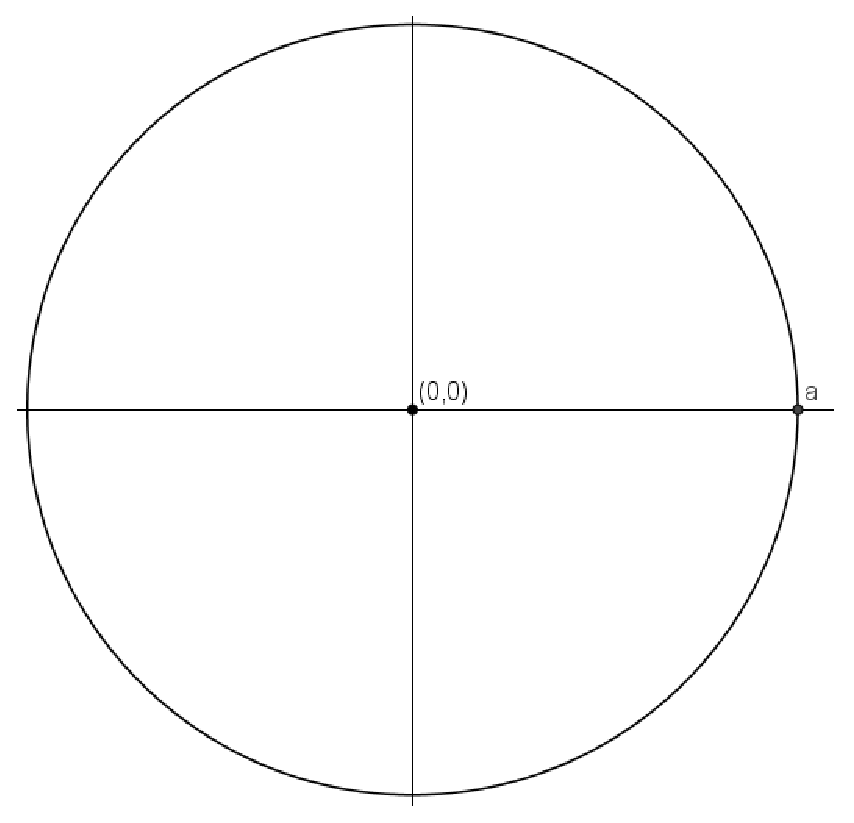
\includegraphics[width=0.2\linewidth]{\dir/Semana14-15/semana14-circulo} \ \ 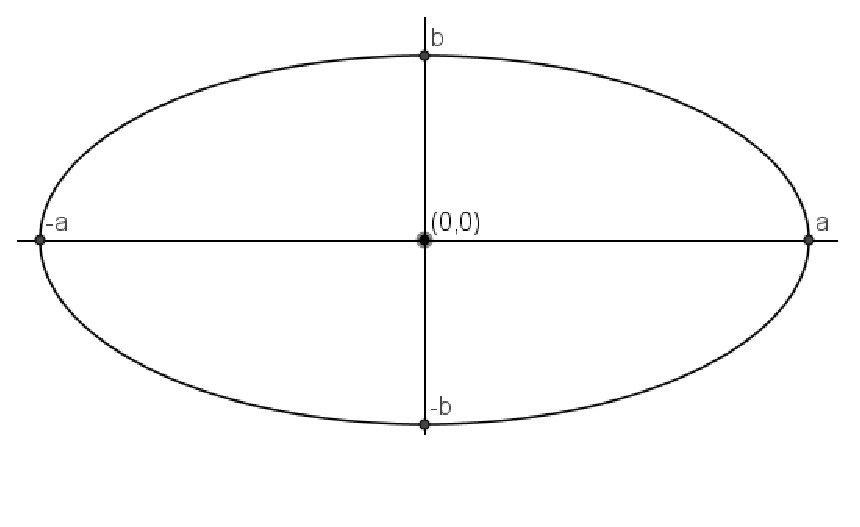
\includegraphics[width=0.3\linewidth]{\dir/Semana14-15/semana14-elipse} \ \ 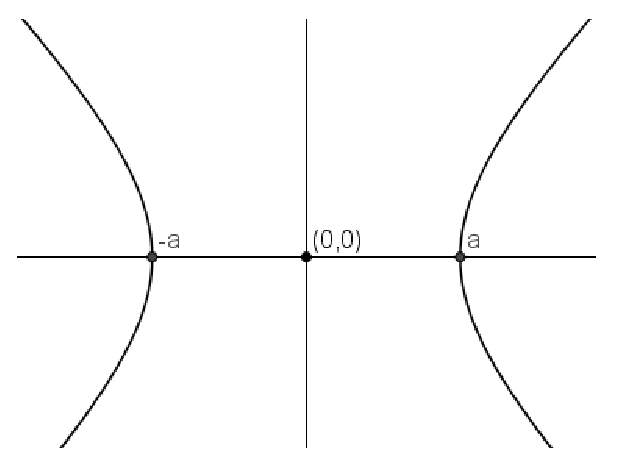
\includegraphics[width=0.3\linewidth]{\dir/Semana14-15/semana14-hiperbole}
	\end{center}
\end{figure}

\noindent Vamos ver como que a diagonalização de formas simétricas se aplica para conseguirmos identificar cônicas de formas quadráticas que possuem termos mistos.


\begin{ex}
	Vamos identificar a cônica cuja equação é
	\begin{equation}
	31 x_1^2 - 10\sqrt{3} x_1x_2 + 21 x_2^2 = 144.
	\end{equation} Podemos escrever
	\begin{equation}
	\vec{x}^T A \vec{x} = 144, \quad \text{onde} \quad
	A = 
	\begin{bmatrix}
	31 & -5\sqrt{3} \\
	-5\sqrt{3} &  21
	\end{bmatrix}.
	\end{equation} Autovalores de $A$:
	\begin{equation}
	p(\lambda) = (31 - \lambda)(21-\lambda) - 75 = 0 \implies \lambda^2 - 52 \lambda + 576
	= 0
	\end{equation}
	\begin{equation}
	\implies \lambda = \frac{52 \pm \sqrt{2704 - 2304}}{2} = \frac{52 \pm 20}{2} = 26\pm 10 \implies \lambda_1 = 16, \ \lambda_2 = 36.
	\end{equation} Autovetores associados:
	\begin{itemize}
		\item  ao autovalor $\lambda_1 = 16$:
		\begin{equation}
		\begin{bmatrix}
		15 & -5\sqrt{3} \\
		-5\sqrt{3} &  5
		\end{bmatrix} \sim
		\begin{bmatrix}
		3 & -\sqrt{3} \\
		0 &  0
		\end{bmatrix} \implies 
		3v_1 = \sqrt{3} v_2 \ \ \xrightarrow[\text{e já normalizando}]{\text{podemos escolher}} \ \  \vec{v}_1 = 
		\begin{bmatrix}
		1/2 \\ \sqrt{3}/2
		\end{bmatrix}.
		\end{equation}
		\item ao autovalor $\lambda_2 = 36$:
		\begin{equation}
		\begin{bmatrix}
		-5 & -5\sqrt{3} \\
		-5\sqrt{3} &  -15
		\end{bmatrix} \sim
		\begin{bmatrix}
		1 & \sqrt{3} \\
		0 &  0
		\end{bmatrix} \implies 
		v_1 = - \sqrt{3} v_2 \ \ \xrightarrow[\text{e já normalizando}]{\text{podemos escolher}} \ \  \vec{v}_2 = 
		\begin{bmatrix}
		-\sqrt{3}/2 \\ 1/2
		\end{bmatrix}.
		\end{equation}
	\end{itemize} Temos
	\begin{equation}
	P^{-1} A P = D =
	\begin{bmatrix}
	16 & 0 \\ 0 & 26
	\end{bmatrix}
	\end{equation} Assim, na base de $\mathbb{R}^2$ determinada por $\{\vec{v}_1, \vec{v}_2\}$, podemos escrever a equação da equação cônica como
	\begin{equation}
	\vec{x}^T A \vec{x} = \vec{y}^T D \vec{y} \implies 
	\begin{bmatrix}
	y_1 & y_2
	\end{bmatrix}
	\begin{bmatrix}
	16 & 0 \\ 0 & 26
	\end{bmatrix}
	\begin{bmatrix}
	y_1 \\ y_2
	\end{bmatrix} = 144.
	\end{equation} Isto pode ser reescrito como
	\begin{equation}
	16 y_1^2 + 36 y_2^2 = 144 \ \leftrightsquigarrow \ \frac{y_1^2}{(144/16)} + \frac{y_1^2}{(144/36)} = 1 \ \leftrightsquigarrow \ \frac{y_1^2}{3^2} + \frac{y_1^2}{2^2} = 1.
	\end{equation} Esta equação é pode ser agora identificada como uma elipse nos ``novos eixos'' $\vec{v}_1$ e $\vec{v}_2$.
	\begin{center}
		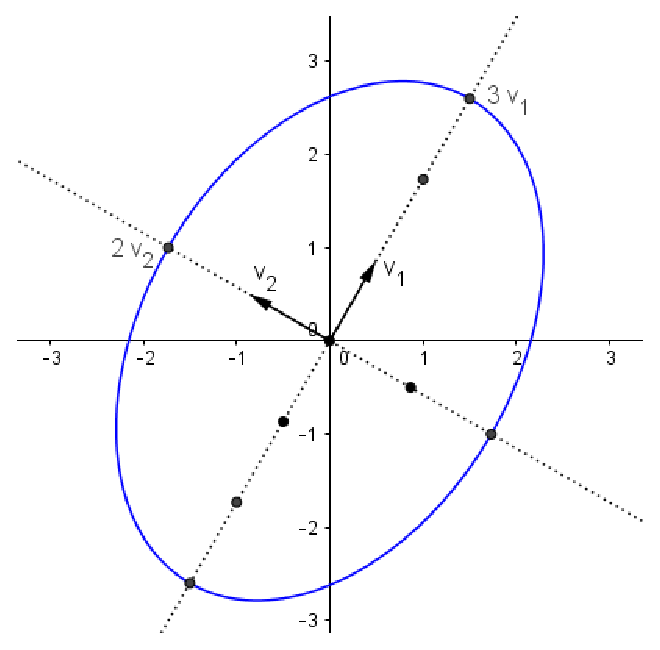
\includegraphics[width=0.5\linewidth]{\dir/Semana14-15/semana14-conicas2}
	\end{center}
	
	\noindent Observamos que quando a coordenada $y_1 = 0$ devemos ter que $y_2^2 = 2^2$, de modo que deve ser $\vec{x} = y_1 \vec{v}_1 + y_2 \vec{v}_2 = \pm 2 \vec{v}_2$, como na figura. Este é o análogo da análise que normalmente fazemos, só que agora na base ortonormal $\{\vec{v}_1, \vec{v}_2\}$
\end{ex}

\subsection*{Exercícios resolvidos}

\construirExeresol

\subsection*{Exercícios}

\construirExer

\section{Problemas de otimização restritos à esfera}

Nesta seção, estudamos alguns problemas de otimização bem específicos. Mais precisamente, podemos encontrar valores de máximo e mínimo de formas quadráticas
\begin{equation}
Q(\vec{x}) = \vec{x}^T A \vec{x}
\end{equation} sujeitos à restrição 
\begin{equation}
x_1^2 + x_2^2 + \cdots + x_n^2 = 1,
\end{equation} que caracteriza os pontos $(x_1, x_2, \dots, x_n) \in \mathbb{R}^n$ que tem comprimento unitário, isto é, a esfera de raio 1 e centro na origem em $\mathbb{R}^n$. Em outras palavras, nosso problema de otimização restrito consiste em achar, na esfera unitária, os vetores em que a forma quadrática $Q$ assume seu maior valor e seu menor valor.

Mais resumidamente, queremos:
\begin{equation}
\text{maximizar/minimizar } Q(\vec{x}) \ \text{sujeito à restrição} \ \|\vec{x}\|=1.
\end{equation}

\noindent \textbf{Ideia por trás do método.} Sendo $A$ uma matriz simétrica, todos os seus autovalores são reais. Vamos ordená-los em forma crescente
\begin{equation}
\lambda_1 \le \lambda_2 \le \cdots \le \lambda_n.
\end{equation} Podemos também encontrar uma base ortonormal de autovetores e, com eles, formar uma matriz ortogonal que diagonaliza $A$:
\begin{equation}
P =  
\begin{bmatrix}
| & | &  & | \\
\vec{v}_1 & \vec{v}_2 & \cdots & \vec{v}_n \\
| & | &  & | \\
\end{bmatrix} \implies
P^{-1} A P = D = 
\begin{bmatrix}
\lambda_1 & 0  & \cdots & 0 \\
0 & \lambda_2  & \cdots & 0 \\
\vdots & \vdots & \ddots & \vdots \\
0 & 0 & \cdots & \lambda_n
\end{bmatrix}.
\end{equation} Nota que $P$, sendo ortogonal, preserva comprimentos (ver Observação \ref{sse} na seção seguinte). Assim, escrevendo $\vec{x} = P \vec{y}$, temos que $\|\vec{x}\| = 1$ se, e somente se, $\|\vec{y}\| = 1$. Além disso, esta matriz $P$ é a matriz ortogonal que diagonaliza $A$, de modo que, pelo que vimos na seção anterior,
\begin{equation}
\vec{x}^T A \vec{x} = \vec{y}^T D \vec{y}.
\end{equation} Mas a forma quadrática $\vec{y}^T D \vec{y}$ é mais fácil de maximizar: sendo $\lambda_n$ a maior das entradas da diagonal principal de $D$, temos (já que cada $\lambda_j \le \lambda_n$ e $\|\vec{y}\| = 1$)
\begin{equation}
\vec{y}^T D \vec{y} = \lambda_1 y_1^2 + \lambda_2 y_2^2 + \cdots + \lambda_n y_n^2 \le  \lambda_n (y_1^2 +y_2^2 + \cdots + y_n^2) = \lambda_n.
\end{equation} Logo, $\lambda_n$ é uma cota superior para $\vec{y}^T D \vec{y}$. Além disso, já que $D$ é uma matriz diagonal, esta cota superior é atingida pelo vetor $\vec{y} = \vec{e}_n$, o último vetor da base canônica de $\mathbb{R}^n$. Traduzindo estas informações para a variável $\vec{x}$, temos que $\lambda_n$ é o valor máximo de $\vec{x}^T A \vec{x}$ (pois é igual a $\vec{y}^T D \vec{y}$) na esfera unitária. Além disso, este valor máximo é atingido quando $\vec{x} = P \vec{e}_n = \vec{v}_n$, um autovetor unitário associado com o maior autovalor $\lambda_n$.

\begin{exer}
	Fazer toda a análise acima para o problema de minimização. \textit{Dica}: olhar para o menor autovalor.
\end{exer}


\begin{ex}\label{otimiz}
	Vamos maximizar a forma quadrática 
	\begin{equation}
	Q(x_1, x_2, x_3) = 7 x_1^2 + x_2^2 + 7x_3^2 - 8 x_1x_2 - 4x_1x_3 - 8 x_2x_3,
	\end{equation} sujeito à restrição $x_1^2 + x_2^2 + x_3^2 = 1$.
	
	Note que podemos escrever
	\begin{equation}
	\vec{x} = 
	\begin{bmatrix}
	x_1 \\ x_2 \\ x_3
	\end{bmatrix} \implies 
	Q(\vec{x}) = \vec{x}^T 
	\begin{bmatrix}
	7 & -4 & -2 \\
	-4 &  1 & -4 \\
	-2 & -4 &  7 \\
	\end{bmatrix}\vec{x}.
	\end{equation} Precisamos determinar o maior autovalor e um autovetor unitário associado. O polinômio característico de $A$ é dado por 
	\begin{equation}
	\det 
	\begin{bmatrix}
	7 - \lambda & -4 & -2 \\
	-4 &  1 - \lambda & -4 \\
	-2 & -4 &  7 - \lambda \\
	\end{bmatrix} = - \lambda^3 + 15 \lambda^2 - 27 \lambda - 243,
	\end{equation} cujas raízes são $\lambda_1 = -3$ e $\lambda_2 = 9$. Portanto, o valor máximo que a forma quadrática $Q$ assume na esfera unitária é $9$.
	
	Além disso, sabemos que qualquer um autovetor unitário associado com o autovalor $\lambda_2 = 9$ assume este valor máximo. Resolvemos
	\begin{equation}
	A - 9 I = 
	\begin{bmatrix}
	-2 & -4 & -2 \\
	-4 & -8 & -4 \\
	-2 & -4 &  -2 \\
	\end{bmatrix} \sim
	\begin{bmatrix}
	1 & 2 & 1 \\
	0 & 0 & 0 \\
	0 & 0 & 0 \\
	\end{bmatrix} \implies \vec{v} =
	\begin{bmatrix}
	-2v_2 - v_3 \\ v_2 \\ v_3
	\end{bmatrix}  = v_2
	\begin{bmatrix}
	-2 \\ 1 \\ 0
	\end{bmatrix} + v_3
	\begin{bmatrix}
	-1 \\ 0 \\ 1
	\end{bmatrix}.
	\end{equation} Um autovetor (unitário!) possível é
	\begin{equation}
	\frac{1}{\sqrt{2}}
	\begin{bmatrix}
	-1 \\ 0 \\ 1
	\end{bmatrix} = 
	\begin{bmatrix}
	-1/\sqrt{2} \\ 0 \\ 1/\sqrt{2}
	\end{bmatrix}.
	\end{equation} Conferimos que 
	\begin{equation}
	Q \left(\frac{1}{\sqrt{2}}, 0, \frac{1}{\sqrt{2}}\right) = \frac{7}{2} + 0 + \frac{7}{2} - 0 + \frac{4}{2} - 0 = 9. \ \lhd
	\end{equation}
\end{ex}


\begin{obs}[Opcional]
	Em cursos de cálculo com várias variáveis, estudamos multiplicadores de Lagrange, uma ferramenta para estudar problemas de otimização com restrição. De uma maneira geral, queremos
	\begin{equation}
	\text{minimizar } f(x_1, x_2, \cdots, x_n) \text{ com a restrição } g(x_1, x_2, \cdots, x_n) = 0.
	\end{equation} O método dos multiplicadores de Lagrange nos dá uma condição necessária: se um ponto é de máximo/mínimo com restrição, então existe uma constante $\lambda$ tal que, neste ponto,
	\begin{equation}
	\vec{\nabla} f = \lambda \vec{\nabla} g.
	\end{equation} Esta constante $\lambda$ é conhecida como um \textbf{multiplicador de Lagrange}. Como mencionamos, esta é uma condição necessária, de modo que não garante que o ponto é de mínimo/máximo. Na prática, depois de encontrarmos os possíveis valores de $\vec{x}$ e de $\lambda$, podemos substituir na função para ver quais são os pontos de mínimo e quais são os de máximo.
	
	Vejamos como esta técnica se aplicaria no Exemplo \ref{otimiz} que já resolvemos acima. Vamos considerar $f(x_1,x_2,x_3) = Q(x_1,x_2,x_3)$ e $g(x_1,x_2,x_3) = x_1^2 + x_2^2 + x_3^2 - 1$ Se estivermos em um ponto de máximo, então existe a constante $\lambda$ como acima. Calculamos:
	\begin{equation}
	\vec{\nabla} Q = \left( 14x_1 - 8x_2 - 4 x_3, 2x_2 - 8 x_1 - 8 x_3, 14x_3 - 4 x_1 - 8 x_2 \right) 
	\end{equation} e 
	\begin{equation}
	\vec{\nabla} g = \left( 2 x_1, 2 x_2, 2 x_3 \right) .
	\end{equation} A condição $\vec{\nabla} Q = \lambda \vec{\nabla} g$ nos diz que devemos resolver
	\begin{equation}
	\begin{array}{c}
	14 x_1 - 8x_2 - 4 x_3 = 2 \lambda x_1 \\
	-8x_1 + 2x_2  - 8 x_3 = 2 \lambda x_2 \\
	- 4x_1 - 8 x_2 +14x_3 = 2 \lambda x_3 \\
	\end{array} \xrightarrow[\text{em cada eq.}]{\text{Simplifica um $2$}}
	\begin{bmatrix}
	7 & -4 & -2 \\
	-4 & 1 & -4 \\
	-2 & -4 & 7 \\
	\end{bmatrix} 
	\begin{bmatrix}
	x_1 \\ x_2 \\ x_3
	\end{bmatrix} = \lambda
	\begin{bmatrix}
	x_1 \\ x_2 \\ x_3
	\end{bmatrix}.
	\end{equation} Chegamos, por outro caminho, à mesma conclusão: $\lambda$ deve ser um autovalor e $\vec{x}$ um autovetor (unitário, já que $g(x_1,x_2,x_3) = 0$) associado$. \ \lhd$
\end{obs}

\subsection*{Exercícios resolvidos}

\construirExeresol

\subsection*{Exercícios}

\construirExer

\section{Matrizes simétricas e prova do Teorema Espectral}

Nesta seção vamos utilizar a notação $\langle \vec{u}, \vec{v} \rangle$ para o produto escalar, ao invés de $\vec{u} \cdot \vec{v}$, para enfatizar qual é o vetor $\vec{u}$ e qual é o vetor $\vec{v}$ (em especial quando um deles está sendo multiplicado por uma matriz).

%Vejamos mais uma maneira equivalente de se dizer que uma matriz é simétrica.
\begin{obs}\label{sse}
	Uma matriz quadrada $A$, não necessariamente simétrica, cujos coeficientes são reais, satisfaz
	\begin{equation}
	\langle A \vec{x}, \vec{y} \rangle = \langle\vec{x}, A^T \vec{y}\rangle, \quad \text{ para todos } \vec{x}, \vec{y} \in \mathbb{R}^n.
	\end{equation} Isto se pode verificar ao analisar os coeficientes de $A \vec{x}$ e de $A^T \vec{y}$. Assim, uma matriz $A$ de ordem $n \times n$ é \textbf{simétrica} se, e somente se, satisfaz
	\begin{equation}
	\langle A \vec{x}, \vec{y} \rangle = \langle\vec{x}, A \vec{y}\rangle, \quad \text{ para todos } \vec{x}, \vec{y} \in \mathbb{R}^n.
	\end{equation}
	Outras formas de escrever esta mesma coisa (concorda?) são
	\begin{equation}
	A \vec{x} \cdot \vec{y} = \vec{x} \cdot A \vec{y}, \quad \text{ para todos } \vec{x}, \vec{y} \in \mathbb{R}^n
	\end{equation} e 
	\begin{equation}
	\vec{y}^T A \vec{x} = \vec{x}^T A \vec{y}, \quad \text{ para todos } \vec{x}, \vec{y} \in \mathbb{R}^n.
	\end{equation}
\end{obs}

\begin{obs}
	A observação anterior nos permite estender a definição de matriz simétrica para transformações lineares, pois é independente do sistema de coordenadas utilizado (depende apenas de uma escolha de produto interno/escalar). 
\end{obs}

A equivalência que foi apresentada na Observação \ref{sse} é muito útil na análise de matrizes simétricas. Vamos ver como se aplica diversas vezes na demonstração do Teorema Espectral que será dividida em três proposições preliminares. Cada uma delas apresenta, em ordem, o procedimento usual que viemos utilizando para diagonalizar matrizes: análise dos autovalores, construção dos autoespaços e verificação de que é possível formar uma base de autovetores. Neste caso de uma matriz simétrica, veremos que, além de tudo, é possível encontrar uma base ortonormal de autovetores.

\begin{prop}\label{reais}
	Os autovalores de uma matriz simétrica $A$, de entradas reais, são números reais.
\end{prop}

\begin{proof}
	Seja $\lambda$ uma raiz do polinômio característico de $A$, que pode ser um número real ou um número complexo. Podemos encontrar um vetor $\vec{v}$, de entradas possivelmente complexas, tal que $A\vec{v} = \lambda \vec{v}$. A menos de um passo de normalização, podemos pensar que $\|\vec{v}\| = 1$. Vamos verificar que de fato $\lambda$ é um número real. Para isto, vamos mostrar que $\lambda$ é igual ao seu conjugado, $\lambda = \bar{\lambda}$, de forma que a parte imaginária de $\lambda$ deve ser igual a zero. Sendo $A$ simétrica, temos que
	\begin{equation}
	\overline{\lambda} = \overline{\lambda \|\vec{v}\|^2} = \overline{\langle \lambda \vec{v}, \vec{v} \rangle} = \overline{\langle A \vec{v}, \vec{v} \rangle} = \overline{\langle \vec{v}, A \vec{v} \rangle} = \overline{\langle \vec{v}, \lambda \vec{v} \rangle} = \lambda \overline{\langle \vec{v}, \vec{v} \rangle} = \lambda.
	\end{equation} A simetria de $A$ foi necessária (apenas) no quarto sinal de igualdade acima. Ainda, na penúltima igualdade, utilizamos sem muitos comentários uma propriedade do produto interno em espaços vetoriais com escalares complexos, a saber, que
	\begin{equation}
	\langle\vec{u}, \vec{v}\rangle \stackrel{\text{def}}{=} \sum_{i=1}^{n} u_i \overline{v}_i.
	\end{equation} Os conjugados das componentes do segundo vetor aparecem para que a fórmula usual para o comprimento continue sendo válida:
	\begin{equation}
	\| \vec{u} \|^2 = \langle\vec{u}, \vec{u}\rangle = \sum_{i=1}^{n} u_i \overline{u}_i = \sum_{i=1}^{n} |u_i|^2.
	\end{equation} Desta forma, continua valendo que
	\begin{equation}
	\langle k\vec{u}, \vec{v} \rangle = k \langle \vec{u}, \vec{v}\rangle, \quad \text{enquanto que} \quad \langle \vec{u},k\vec{v}\rangle = \overline{k} \langle \vec{u}, \vec{v}\rangle. \qedhere
	\end{equation}
\end{proof}

\begin{prop}\label{ortog}
	Se $A$ é uma matriz simétrica, então autovetores associados a autovalores distintos são ortogonais.
\end{prop}

\begin{proof}
	Sejam $\lambda_1$ e  $\lambda_2$ autovalores distintos de $A$ e $\vec{v}_1, \vec{v}_2$ respectivos autovetores. Então (observe que é necessário que $A$ seja simétrica na segunda e na última igualdade!)
	\begin{equation}
	\lambda_1 \langle \vec{v}_1, \vec{v}_2\rangle = \langle \lambda_1 \vec{v}_1, \vec{v}_2\rangle = \langle A \vec{v}_1, \vec{v}_2\rangle = \langle \vec{v}_1, A \vec{v}_2\rangle = \overline{\lambda}_2 \langle \vec{v}_1, \vec{v}_2\rangle = \lambda_2 \langle \vec{v}_1, \vec{v}_2\rangle,
	\end{equation} de modo que $(\lambda_1 - \lambda_2)\langle \vec{v}_1, \vec{v}_2\rangle = 0$. Já que estamos supondo que os autovalores são distintos, $\lambda_1 \neq \lambda_2$, concluimos que $\langle \vec{v}_1, \vec{v}_2\rangle = 0$.
\end{proof}


\begin{prop}\label{dimens}
	Seja $A$ uma matriz simétrica. Então, a dimensão do autoespaço associado a um autovalor é igual à multiplicidade deste autovalor.
\end{prop}

\begin{proof}
	Suponhamos que $\lambda_1$ é um autovalor de $A$ de multiplicidade $k$. Seja $\vec{v}_1$ um autovetor unitário associado. Podemos encontrar uma base ortonormal de $\mathbb{R}^n$ da qual $\vec{v}_1$ faz parte, isto é, podemos encontrar vetores unitários $\vec{y}_j$ de modo que
	\begin{equation}
	\{ \vec{v}_1, \vec{y}_2, \vec{y}_3, \dots, \vec{y}_n \}
	\end{equation} é uma base ortonormal de $\mathbb{R}^n$.
	
	Considere a matriz $Q$ cujas colunas são os elementos desta base:
	\begin{equation}
	Q = 
	\begin{bmatrix}
	| & | & | & & | \\
	\vec{v}_1 & \vec{y}_2 & \vec{y}_3 & \cdots &  \vec{y}_n \\
	| & | & | & & | \\
	\end{bmatrix},
	\end{equation} que é, consequentemente, ortogonal. Vamos calcular $Q^{-1} A Q = Q^T A Q$. O produto $AQ$ pode ser interpretado como o produto de $A$ por cada uma das colunas de $Q$:
	\begin{equation}
	AQ = 
	\begin{bmatrix}
	| & | & | & & | \\
	A \vec{v}_1 & A \vec{y}_2 & A \vec{y}_3 & \cdots &  A\vec{y}_n \\
	| & | & | & & | \\
	\end{bmatrix} = 
	\begin{bmatrix}
	| & | & | & & | \\
	\lambda_1 \vec{v}_1 & A \vec{y}_2 & A \vec{y}_3 & \cdots &  A\vec{y}_n \\
	| & | & | & & | \\
	\end{bmatrix}.
	\end{equation} Logo,
	\begin{equation}
	Q^TAQ =
	\begin{bmatrix}
	\text{---} & \vec{v}_1 & \text{---} \\
	\text{---} & \vec{y}_2 & \text{---} \\
	\text{---} & \vec{y}_3 &\text{---} \\
	& \vdots    &     \\
	\text{---} & \vec{y}_n & \text{---} \\      
	\end{bmatrix}
	\begin{bmatrix}
	| & | & | & & | \\
	\lambda_1 \vec{v}_1 & A \vec{y}_2 & A \vec{y}_3 & \cdots &  A\vec{y}_n \\
	| & | & | & & | \\
	\end{bmatrix}
	\end{equation}
	\begin{equation}
	\implies Q^TAQ =
	\begin{bmatrix}
	\lambda_1\langle \vec{v}_1, \vec{v}_1 \rangle & \langle \vec{v}_1, A\vec{y}_2 \rangle & \langle \vec{v}_1, A\vec{y}_3 \rangle & \cdots & \langle \vec{v}_1, A\vec{y}_n \rangle \\
	\lambda_1\langle \vec{y}_2, \vec{v}_1 \rangle & \langle \vec{y}_2, A\vec{y}_2 \rangle & \langle \vec{y}_2, A\vec{y}_3 \rangle & \cdots & \langle \vec{y}_2, A\vec{y}_n \rangle \\
	\lambda_1\langle \vec{y}_3, \vec{v}_1 \rangle & \langle \vec{y}_3, A\vec{y}_2 \rangle & \langle \vec{y}_3, A\vec{y}_3 \rangle & \cdots & \langle \vec{y}_3, A\vec{y}_n \rangle \\
	\vdots & \vdots & \vdots & \ddots & \vdots \\
	\lambda_1\langle \vec{y}_n, \vec{v}_1 \rangle & \langle \vec{y}_n, A\vec{y}_2 \rangle & \langle \vec{y}_n, A\vec{y}_3 \rangle & \cdots & \langle \vec{y}_n, A\vec{y}_n \rangle \\
	\end{bmatrix}
	\end{equation} Observamos que, pela simetria de $A$ e por ser $	\{ \vec{v}_1, \vec{y}_2, \vec{y}_3, \dots, \vec{y}_n \}$ um conjunto ortonormal, temos 
	\begin{equation}
	\langle \vec{v}_1, A\vec{y}_j \rangle = \langle A\vec{v}_1, \vec{y}_j \rangle = \lambda_1 \langle \vec{v}_1, \vec{y}_j \rangle = 0, \quad \text{para qualquer índice } j.
	\end{equation}Logo,
	\begin{equation}
	\implies Q^TAQ =
	\begin{bmatrix}
	\lambda_1 & 0 & 0 & \cdots & 0 \\
	0 & b_{22} & b_{23} & \cdots & b_{2n} \\
	0 & b_{32} & b_{33} & \cdots & b_{3n} \\
	\vdots & \vdots & \vdots & \ddots & \vdots \\
	0 & b_{n2} & b_{n3} & \cdots & b_{nn} \\
	\end{bmatrix} \stackrel{\text{def}}{=} \hat{A}.
	\end{equation} Chamamos os coeficientes restantes de $b_{ij}$ simplesmente porque não nos interessa muito quanto valem (notamos, no entanto, que a simetria de $A$ implica que $b_{ij} = b_{ji}$). Observamos que 
	\begin{equation}
	\det \left( A - \lambda I \right) = \det \left( Q^{-1} (A - \lambda I) Q \right) =	\det \left( \hat{A} - \lambda I \right) = (\lambda_1 - \lambda) \cdot \det (B - \lambda I),
	\end{equation} onde $B$ é a matriz de ordem $(n-1)\times (n-1)$ dada por $(b_{ij})$. Além disso, se a multiplicidade de $\lambda_1$ como autovalor de $A$ for maior do que $1$, devemos ter, pela igualdade acima, que $\lambda_1$ também é um autovalor de $B$. Desta forma, $\hat{A}$ possui um autovetor unitário $\vec{v}_2$ associado com $\lambda_1$ que está contido em $\Span \{ \vec{y}_2, \vec{y}_3, \dots, \vec{y}_n \}$ e, portanto, é distinto e linearmente independente a $\vec{v}_1$. O processo de Gram-Schmidt permite obter $\{\vec{v}_1, \vec{v}_2\}$ ortonormais.
	
	A partir daí, repetimos o processo completando o conjunto $\{\vec{v}_1, \vec{v}_2\}$ a uma base ortonormal $\{ \vec{v}_1, \vec{v}_2, \vec{y}_3, \dots, \vec{y}_n \}$ de $\mathbb{R}^n$. Daí vamos obter um terceiro autovetor ortogonal aos anteriores e unitário. Procedemos desta meneira até encontrar $k$ autovetores ortogonais e unitários associados ao autovalor $\lambda_1$. Assim, o autoespaço $\operatorname{Nul} (A - \lambda_1 I)$ tem dimensão $k$, que é igual à multiplicidade do autovalor $\lambda_1$.
\end{proof}

\subsection{Prova do Teorema Espectral}

O Teorema Fundamental da Álgebra afirma que todo polinômio não constante de grau $n$ possui exatamente $n$ raízes complexas. Sendo assim, qualquer matriz $A$ de ordem $n\times n$ possui $n$ autovalores complexos. No entanto, sendo $A$ uma matriz simétrica, a Proposição \ref{reais} garante que todas estes $n$ autovalores são todos reais. Vamos denotar por
\begin{equation}
\lambda_1, \lambda_2, \dots, \lambda_k \in \mathbb{R}
\end{equation} os autovalores distintos de $A$ e por $m_1, m_2, \dots, m_k$ suas respectivas multiplicidades. Temos, em particular, que $m_1 + m_2 + \cdots + m_k = n$.

Pela Proposição \ref{dimens}, a dimensão do autoespaço associado a $\lambda_1$ é $m_1$. Podemos encontrar (da maneira usual, por escalonamento) uma base de autovetores
\begin{equation}
\operatorname{Nul} (A - \lambda_1 I) = \Span \{ \vec{u}_1, \vec{u}_2, \dots, \vec{u}_{m_1} \}.
\end{equation} Estes autovetores, possivelmente não são ortogonais, mas, aplicando o Processo de Gram-Schmidt, podemo obter uma base ortonormal de $\operatorname{Nul} (A - \lambda_1 I)$:
\begin{equation}
\operatorname{Nul} (A - \lambda_1 I) = \Span \{ \vec{v}_1, \vec{v}_2, \dots, \vec{v}_{m_1} \}.
\end{equation} Fazendo este mesmo procedimento para cada um dos autovalores, obtemos $n$ autovetores, que, consequentemente, formam uma base para $\mathbb{R}^n$. Logo, $A$ é diagonalizável.

Além disso, a Proposição \ref{ortog} garante que todo autovetor de um autoespaço é ortogonal a todo autovetor de outro autoespaço (associado a um autovalor diferente). Temos então $k$ autoespaços, cujas bases são ortonormais e elementos da base de um autoespaço são ortogonais aos elementos das outras bases. Segue daí que a união das bases dos autoespaços, como consideramos, é uma base \textit{ortonormal} para $\mathbb{R}^n$.

Explicitamente, a matriz
\begin{equation}
P = 
\begin{bmatrix}
| & | & & | \\
\vec{v}_1 & \vec{v}_2 & \cdots &  \vec{v}_n \\
| & | &  & | \\
\end{bmatrix}
\end{equation} formada pelos autovetores é ortogonal e 
\begin{equation}
P^{-1} A P = D = 
\begin{bmatrix}
\lambda_1 & 0 & 0 & \cdots & 0 \\ 
0 & \lambda_2 & 0 & \cdots & 0 \\ 
0 & 0 & \lambda_3 & \cdots & 0 \\ 
\vdots & \vdots & \vdots & \ddots & \vdots \\ 
0 & 0 & 0 & \cdots & \lambda_n \\ 
\end{bmatrix}.
\end{equation} Sendo $P$ ortogonal, tem-se ainda que $P^{-1} = P^T$.

\subsection*{Exercícios resolvidos}

\construirExeresol

\subsection*{Exercícios}

\construirExer

\section{Exercícios finais}

\construirExer

%\end{document} 


%resposta dos exercícios
\ifisbook
\include{respostas}
\fi

%references
\nocite{*}
\bibliographystyle{plain}
\bibliography{main}
\addcontentsline{toc}{chapter}{Referências Bibliográficas}
\fancyhead[RE]{Álgebra Linear}
\fancyhead[LO]{REFERÊNCIAS BIBLIOGRÁFICAS}
\fancyhead[LE,RO]{\thepage}

\ifisbook
\clearpage
\addcontentsline{toc}{chapter}{Índice Remissivo}
\fancyhead[RE]{Álgebra Linear}
\fancyhead[LO]{ÍNDICE REMISSIVO}
\fancyhead[LE,RO]{\thepage}
\printindex
\fi

\end{document}
